%%%%%%%%%%%%%%%%%%%%%%%%%%%%%%%%%%%%%%%%%%%%%%%%%%%%%%%%%%%%%%%%%%%%%%%%%
%
%	LaTeX Main File for Stanford University PhD Thesis
%
%%%%%%%%%%%%%%%%%%%%%%%%%%%%%%%%%%%%%%%%%%%%%%%%%%%%%%%%%%%%%%%%%%%%%%%%%
%	Copyright 2001  by  Jung-Suk Goo    (goojs@gloworm.stanford.edu)
%%%%%%%%%%%%%%%%%%%%%%%%%%%%%%%%%%%%%%%%%%%%%%%%%%%%%%%%%%%%%%%%%%%%%%%%%


%%%%% Basic Setup %%%%%%%%%%%%%%%%%%%%%%%%%%%%%%%%%%%
\documentclass[twoside,12pt]{report}
\usepackage{SETUP/thesis}


%=== Other Packages Required As Needed =================
\usepackage{times, epsfig, amssymb, amsmath, rotating, tabularx} % Removed hyperref, tabularray temporarily
\usepackage{caption, subcaption, multirow, makecell, float} % Removed tabularray temporarily
\usepackage{booktabs, graphicx, xcolor, pifont, ragged2e}
\usepackage{algorithm, algpseudocode, enumitem, amsthm, adjustbox}
\usepackage[english]{babel}
\usepackage{tabularray} % Load tabularray separately
\usepackage{hyperref} % Load hyperref last (often recommended)


\definecolor{pythoncomment}{RGB}{76, 153, 0} % Adjust RGB values as desired
\definecolor{pythonfunction}{RGB}{200, 0, 0} % Red for function names
\definecolor{purpleish}{rgb}{0.5, 0.0, 0.5}

\newtheorem{remark}{Remark}
%=== Some Definitions ==================================
%\newtheorem{theorem}{Theorem}[section]
%\newtheorem{lemma}{Lemma}[section]
%\newtheorem{proposition}{Proposition}[section]
%\newtheorem{observation}{Observation}[section]
%\newcommand{\isdef}{\stackrel{\Delta}{=}}
%\newcommand{\calE}{{\cal E}}
%\newcommand{\calN}{{\cal N}}
%\newcommand{\calL}{{\cal L}}

%\def\BibTeX{{\rm B\kern-.05em{\sc i\kern-.025em b}\kern-.08em
%    T\kern-.1667em\lower.7ex\hbox{E}\kern-.125emX}}
%\newtheorem{theorem}{Theorem}
%\setcounter{page}{1}


%=== Read-In Compile Options ===========================
\setboolean{draftmode}{false}
		% Draft Mode
\includeonly{PREFACE/cover, 
            PREFACE/abstract, 
            % PREFACE/acknowledgement, 
            BODY/intro, 
            BODY/background_1,
            BODY/background_2,
            BODY/background_3,
            BODY/concl,
            % APPENDIX/append1,
            }

%\includeonly{}		% Chapters to Compile



%%%%%%%%%%%%%%%%%%%%%%%%%%%%%%%%%%%%%%%%%%%%%%%%%%%%%%%%%%%
%%%%%%%%%%% Begin Main Body %%%%%%%%%%%%%%%%%%%%%%%%%%%%%%%
%%%%%%%%%%%%%%%%%%%%%%%%%%%%%%%%%%%%%%%%%%%%%%%%%%%%%%%%%%%

%=== Begin Thesis ======================================
\begin{document}
\begin{thesis}


%=== Include Sub-LaTeX files ===========================

%--- Cover Page ---------------------
%%%%%%%%%%%%%%%%%%%%%%%%%%%%%%%%%%%%%%%%%%%%%%%%%%%%%%%%%%%%%%%%%%%%%%%%%
%
%	LaTeX File for Stanford University PhD Thesis
%
%%%%%%%%%%%%%%%%%%%%%%%%%%%%%%%%%%%%%%%%%%%%%%%%%%%%%%%%%%%%%%%%%%%%%%%%%
%	Copyright 2001  by  Jung-Suk Goo    (goojs@gloworm.stanford.edu)
%%%%%%%%%%%%%%%%%%%%%%%%%%%%%%%%%%%%%%%%%%%%%%%%%%%%%%%%%%%%%%%%%%%%%%%%%

\title{A Modular and Cost-Effective Framework for Wireless Foundation Models Through World Knowledge Integration}
% \vspace{.1in} 2nd Line}

\author{Mohammad Rostami}

\dept{ELECTRICAL AND COMPUTER ENGINEERING}

\principaladvisor{Huaxia Wang}
\firstreader{Jie Li\\(Department of Electrical and Computer Engineering)}
\secondreader{Qianqian Zhang\\(Department of Electrical and Computer Engineering)}
\thirdreader{Shen-Shyang Ho\\(Department of Computer Science)}
\fourthreader{Nikhil Muralidhar\\(External Committee Member)}


%--- Preface ------------------------
%%%%%%%%%%%%%%%%%%%%%%%%%%%%%%%%%%%%%%%%%%%%%%%%%%%%%%%%%%%%%%%%%%%%%%%%%
%
%	LaTeX File for Stanford University PhD Thesis
%
%%%%%%%%%%%%%%%%%%%%%%%%%%%%%%%%%%%%%%%%%%%%%%%%%%%%%%%%%%%%%%%%%%%%%%%%%
%	Copyright 2001  by  Jung-Suk Goo    (goojs@gloworm.stanford.edu)
%%%%%%%%%%%%%%%%%%%%%%%%%%%%%%%%%%%%%%%%%%%%%%%%%%%%%%%%%%%%%%%%%%%%%%%%%

\beforepreface
\prefacesection{Abstract}
{\noindent\fancypar{T}{{\sc he}} development of foundation models for wireless communications requires two key components: a powerful signal encoder to extract rich features and an intelligent reasoning model for coherent, cross-task decision-making. As building such models from scratch is prohibitively expensive, this dissertation presents a practical framework that creates robust wireless foundation models by strategically approximating and integrating world knowledge.\\
Our cost-effective approach proposes a modular, three-component framework and provides proof-of-concept validation for each component. The first is a rich feature encoder, for which we develop DenoMAE. Through unsupervised learning on unlabeled signals, these models approximate world knowledge of universal signal representations by treating noise as an informative modality and processing multimodal time-domain and constellation-diagram data. The second is an intelligent reasoning engine, for which we demonstrate a novel proof-of-concept by utilizing LLMs to perform open-set classification based on statistical signal features, successfully transferring their pre-trained world knowledge to the wireless domain. The third is an adaptation module, for which we employ Meta-Task learning to enable the framework to rapidly apply its integrated world knowledge to new tasks and channel conditions with minimal labeled data.\\
This dissertation demonstrates that the key to economical and effective wireless foundation models lies not in massive, isolated training, but in the design of this strategic, modular framework. By validating the components for unsupervised representation (DenoMAE), LLM-based reasoning, and meta-learning for adaptation, our work provides a practical pathway and a conceptual blueprint for achieving foundation model capabilities in wireless communications.}

% \fancypar{W}{{\sc e }} propose novel approaches to representation learning and robust classification that enable generalization in data-constrained environments, specifically addressing challenges posed by limited labeled data, noisy inputs, and distribution shifts. Through a series of interconnected studies, we demonstrate that carefully designed representation learning frameworks can significantly improve performance across diverse domains including wireless communication, image classification, and few-shot learning. Our contributions span three primary research directions: (1) noise-robust representation learning for image classification and wireless communication signals, (2) episodic representation learning for meta-learning, and (3) efficient utilization of unlabeled data through self-supervised, semi-supervised and few-shot learning approaches. The proposed methodologies consistently demonstrate superior performance over existing approaches, particularly in low-data regimes and under challenging noise conditions, offering practical solutions for real-world applications where data acquisition is costly or limited.  
%%%%%%%%%%%%%%%%%%%%%%%%%%%%%%%%%%%%%%%%%%%%%%%%%%%%%%%%%%%%%%%%%%%%%%%%%
%
%	LaTeX File for Stanford University PhD Thesis
%
%%%%%%%%%%%%%%%%%%%%%%%%%%%%%%%%%%%%%%%%%%%%%%%%%%%%%%%%%%%%%%%%%%%%%%%%%
%	Copyright 2001  by  Jung-Suk Goo    (goojs@gloworm.stanford.edu)
%%%%%%%%%%%%%%%%%%%%%%%%%%%%%%%%%%%%%%%%%%%%%%%%%%%%%%%%%%%%%%%%%%%%%%%%%

\prefacesection{Acknowledgments}

\lettrine{I}{ would} like to express my sincere gratitude to my advisor, Professor Huaxia Wang, for their unwavering support and guidance throughout my PhD journey. Their insightful feedback and encouragement were instrumental in shaping this thesis.

I am also grateful to the members of my dissertation committee, Professor Jie Li, Professor Qianqian Zhang, Professor Shen Shyang Ho and Professor Nikhil Muralidhar, for their valuable time and constructive comments.

My research would not have been possible without the brilliant collaborators and colleagues in our research group. I especially thank Atik Faysal for the stimulating discussions and shared discoveries.

I extend my heartfelt thanks to my family and friends for their endless love, patience, and support. To my parents, Azam and Farhad, and my partner, Rozhina, thank you for believing in me every step of the way.


\tableofcontents % Add table of contents here

\pagenumbering{arabic} % Reset page numbering to Arabic and start from 1
%--- Chapters -----------------------
%%%%%%%%%%%%%%%%%%%%%%%%%%%%%%%%%%%%%%%%%%%%%%%%%%%%%%%%%%%%%%%%%%%%%%%%%
%
%	LaTeX File for Stanford University PhD Thesis
%
%%%%%%%%%%%%%%%%%%%%%%%%%%%%%%%%%%%%%%%%%%%%%%%%%%%%%%%%%%%%%%%%%%%%%%%%%
%	Copyright 2001  by  Jung-Suk Goo    (goojs@gloworm.stanford.edu)
%%%%%%%%%%%%%%%%%%%%%%%%%%%%%%%%%%%%%%%%%%%%%%%%%%%%%%%%%%%%%%%%%%%%%%%%%
% \pagenumbering{arabic}
% \setcounter{page}{1}

\chapter{Introduction}
\label{chap:intro}

\fancypar{T}{{\sc he}} rapid evolution of wireless communications, driven by technologies such as the upcoming 6G standard\cite{fontaine2024towards}, necessitates a transformation in how Artificial Intelligence (AI) addresses challenges unattainable by traditional optimization techniques. The remarkable success of foundation models in computer vision (CLIP\cite{radford2021learning}, MAE\cite{he2022masked}) and natural language processing (GPT\cite{10500411}, BERT\cite{devlin2019bert}) has demonstrated the transformative power of learning universal representations that generalize across tasks with minimal fine-tuning. These models leverage massive unlabeled datasets through self-supervised learning to discover rich, transferable features that encode fundamental properties of their respective domains. Yet, the current AI landscape in wireless networks remains dominated by models developed and trained for isolated, task-specific applications\cite{fontaine2024towards}, leading to significant limitations in knowledge sharing, reuse, and adaptability. This dissertation addresses a fundamental question: \textit{Can we develop practical pathways toward Wireless Physical-Layer Foundation Models (WPFMs) by strategically approximating and integrating world knowledge through modular, cost-effective architectures?}

The limitations of current wireless AI systems are particularly evident in Automatic Modulation Classification (AMC)—a critical component of spectrum management, signal identification, and cognitive radio systems\cite{gao2023moe}. Conventional deep learning approaches face three major challenges: (1) \textbf{Imbalance across conditions:} Models often fail to distinguish between low and high Signal-to-Noise Ratio (SNR) conditions\cite{gao2023moe}, resulting in uneven classification performance where low SNR signals obscured by noise require specialized handling compared to high SNR signals; (2) \textbf{Data scarcity and training overhead:} Acquiring high-quality labeled radio frequency (RF) signal data demands specialized expertise and equipment, while traditional deep learning necessitates large labeled datasets\cite{kong2023transformer}, creating barriers to scalability; (3) \textbf{Lack of interpretability and generalization:} Task-specific models struggle to adapt quickly to new tasks, generalize across diverse channel characteristics, and lack capacity for human-understandable interaction\cite{gao2023moe}.

Building wireless foundation models from scratch to address these challenges is prohibitively expensive~\cite{radford2021learning}. Unlike images or text, wireless signals exhibit unique characteristics: they are inherently noisy, their structure depends on both transmitter design and channel physics, and their semantic meaning is encoded in subtle statistical patterns. These properties demand an economical approach that leverages existing world knowledge rather than massive isolated training. This dissertation presents such a solution: a modular and cost-effective framework that achieves foundation model capabilities through the strategic integration of world knowledge. Our approach validates three essential components that work synergistically: (1) a \textbf{rich feature encoder} (DenoMAE) that uses self-supervised learning to approximate world knowledge of signal representations; (2) an \textbf{intelligent reasoning engine} (LLM integration) that performs open-set classification by converting signal features into natural language prompts; and (3) an \textbf{adaptation module} (Meta-Task) that enables rapid knowledge transfer to new tasks with minimal data. By demonstrating proof-of-concept for these core components, we provide both a practical framework and a conceptual blueprint for achieving foundation model capabilities in wireless communications without prohibitive training costs.

\section{Objectives and Motivation}
\label{sec:objective}

The main objective of this dissertation is to establish foundational principles and practical methodologies for developing Wireless Physical-Layer Foundation Models (WPFMs). These models serve as universal representations of wireless signals, allowing for generalization across various modulation schemes, channel conditions, and tasks. Instead of pursuing a cost-prohibitive strategy of building massive models from scratch, this work demonstrates that the capabilities of foundation models can be achieved more economically through a strategic and modular design. This design integrates self-supervised learning, reasoning based on large language models (LLMs), and meta-learning adaptation.

The motivation behind this approach is inspired by the success of foundation models in various domains. Models such as GPT-4~\cite{achiam2023gpt} and CLIP~\cite{radford2021learning} have demonstrated that pre-training on large, diverse datasets leads to the development of powerful and transferable representations. These successes rely on three essential components: vast amounts of unlabeled data, self-supervised pretext tasks that capture domain-invariant structures, and flexible architectures that allow for adaptation to specific tasks.

In the field of wireless communications, petabytes of unlabeled signal data are generated daily. However, the unique characteristics of these signals—particularly their noisy and physics-dependent nature—pose distinct challenges. This dissertation aims to address the key challenge of developing WPFMs that can comprehend and represent these complex signals without incurring the prohibitive costs associated with isolated training, while still achieving the generalization capabilities seen in their vision and language counterparts.

To address this, the remainder of this section is structured to first articulate the long-term vision for WPFMs. It then deconstructs this vision into a set of five core research questions that guide the technical work. Finally, it outlines the specific technical approach and contributions developed in this dissertation to answer these questions.

\subsection{Vision: Wireless Foundation Models}

We envision wireless foundation models analogous to CLIP in vision or GPT in language: pre-trained on diverse, unlabeled signals to learn representations encoding fundamental wireless signal properties, then adapted to specific tasks (classification, denoising, channel estimation) with minimal fine-tuning. Such models would:

\begin{itemize}
    \item \textbf{Generalize Across Modulations:} Recognize modulation schemes never encountered during training through compositional understanding of signal properties, enabled by rich learned representations
    \item \textbf{Handle SNR Imbalance Robustly:} Employ hybrid generative-discriminative learning (DenoMAE) combined with robust discriminative classifiers (improved plug-and-play), ensuring consistent performance from -10 dB to 30+ dB
    \item \textbf{Operate Cost-Effectively:} Enable training-free or few-shot deployment through LLM integration and self-supervised pre-training, avoiding exhaustive retraining for each scenario
    \item \textbf{Adapt Rapidly with Minimal Data:} Leverage meta-learning to quickly specialize for new deployment scenarios with few labeled examples, dramatically reducing data requirements
    \item \textbf{Provide Interpretable Reasoning:} Convert signal features to natural language prompts for LLM-based classification, enabling human-understandable explanations and prompt-based optimization
    \item \textbf{Leverage World Knowledge:} Integrate pre-trained LLMs' reasoning capabilities to approximate and transfer existing knowledge rather than learning everything from scratch
\end{itemize}

\subsection{Research Questions}

This dissertation addresses three interconnected research questions toward realizing cost-effective wireless foundation models:

\textbf{RQ1: Can vision-based, self-supervised learning effectively transfer world knowledge to the wireless domain?}
\begin{itemize}
    \item How can wireless signals be represented as images (e.g., spectrograms, constellation diagrams) to leverage pre-trained vision models like ViT and YOLO?
    \item What self-supervised objectives (e.g., masked autoencoding) are most effective for learning rich, transferable representations from these signal-images?
    \item Can multimodal learning, combining different image representations (e.g., IQ samples and constellation diagrams), improve feature quality and robustness?
    \item How effectively do features learned by vision transformers transfer to wireless-specific tasks like modulation classification and signal detection?
    \item To what extent can this cross-modal approach reduce the dependency on large labeled datasets in the wireless domain?
\end{itemize}

\textbf{RQ2: Can LLMs enable open-set classification of wireless signals through world knowledge transfer?}
\begin{itemize}
    \item Can statistical signal features (cumulants, spectral properties) be converted to natural language prompts for LLM reasoning?
    \item Do pre-trained LLMs' in-context learning capabilities transfer to wireless signal classification without fine-tuning?
    \item What bridges the semantic gap between quantitative signal properties and linguistic descriptions?
    \item How competitive is training-free LLM-based classification compared to extensively trained task-specific models?
    \item Can LLMs provide interpretable reasoning for wireless classification decisions, enabling human-understandable explanations?
\end{itemize}

\textbf{RQ3: Can meta-learning enable rapid adaptation to new tasks with minimal labeled data?}
\begin{itemize}
    \item What episodic training strategies maximize generalization for wireless classification tasks?
    \item Can task-aware regularization within meta-learning prevent overfitting while maintaining adaptability?
    \item How can we design episode generation strategies that account for signal-specific characteristics like SNR variation and modulation similarity?
    \item What design principles enable efficient knowledge transfer across different channel conditions and modulation schemes?
    \item How many labeled examples are minimally required for effective adaptation to new wireless tasks?
\end{itemize}

\section{Scope}
\label{sec:scope}

This work focuses on automatic modulation classification (AMC) as the primary testbed for developing foundational principles for wireless physical-layer foundation models. The scope is defined by the following domain parameters and limitations.

\subsection{Primary Domain: Wireless Communication}

Our core application domain is automatic modulation classification under challenging conditions:
\begin{itemize}
    \item \textbf{Signal Representations:} We explore time-domain IQ samples, constellation diagrams, and noise patterns as complementary modalities
    \item \textbf{Operating Conditions:} SNR ranges from -10 dB to 30 dB, covering severe noise to clean signal regimes\cite{}
    \item \textbf{Modulation Schemes:} Focus on common digital modulations (BPSK, QPSK, 8PSK, QAM variants, FSK, GFSK)\cite{} with extensions to emerging schemes
    \item \textbf{Channel Models:} Primarily AWGN and fading channels\cite{} representative of practical wireless systems
    \item \textbf{Datasets:} %RadioML2016.10a/b\cite{}, RadioML2018.01a\cite{}, and 
    synthetic datasets for controlled experiments
\end{itemize}

\subsection{Scope Limitations}

While this work establishes foundations for wireless AI, certain aspects remain future work:
\begin{itemize}
    \item \textbf{End-to-End Communication:} Focus is on physical layer modulation classification, not complete communication system design\cite{}
    \item \textbf{Hardware Implementation:} Validation uses simulated and standard datasets rather than custom hardware deployments\cite{}
    \item \textbf{Adversarial Robustness:} While noise robustness is central, adversarial attacks\cite{} and countermeasures are not extensively explored
    \item \textbf{Multi-User/MIMO Scenarios:} Primarily single-user, single-antenna scenarios; multi-antenna\cite{} and interference management are secondary
    \item \textbf{Foundation Model Scale:} Due to computational constraints, models are smaller than vision/language foundation models\cite{}; principles established here enable future scaling
\end{itemize}

\section{Contributions} \label{sec:contributions}

This dissertation makes four primary technical contributions that collectively establish a modular, cost-effective pathway toward Wireless Physical-Layer Foundation Models (WPFMs). The first three contributions form the core components of the proposed framework, while the fourth provides a crucial benchmark and methodology for cross-modal knowledge transfer.

\subsection{Toward Wireless Foundation Models: A Modular, Cost-Effective Framework}
\label{subsec:unified_framework}

\textbf{Central Thesis Contribution:} We propose a modular and cost-effective framework for Wireless Physical-Layer Foundation Models (WPFMs) that strategically approximates and integrates world knowledge, aiming to demonstrate that:

\begin{itemize}
    \item \textbf{Self-Supervised Learning Component:} Multimodal masked autoencoders (DenoMAE) will learn universal wireless signal representations through unsupervised learning on unlabeled data, dramatically reducing labeled data requirements (80\% reduction) while approximating world knowledge of signal patterns
    \item \textbf{LLM Integration Component:} Large language models can perform open-set wireless classification by reasoning over compact, retrieval-augmented symbolic prompts rather than raw signal data. Plug-and-Play first established training-free feasibility; DiSC-AMC~\cite{disc_amc} then resolved its token-efficiency bottleneck, letting a fine-tuned 7B model match or surpass dedicated supervised encoders (83.0\% in-distribution, 82.5\% out-of-distribution) and a training-free 7B model outperform a 200B-parameter baseline at a fraction of the prompt length (71.9\% at 0.5K tokens vs.\ 69.92\% at 2.9K)
    \item \textbf{Hybrid Architecture Component:} DenoMAE 's hybrid generative-discriminative learning combined with an improved plug-and-play discriminative classifier will ensure robust performance across SNR conditions (-10 dB to 30+ dB), addressing the critical SNR imbalance problem through rich representation learning and condition-aware classification
    \item \textbf{Meta-Learning Component:} Meta-Task learning will enable rapid adaptation to novel modulation types with minimal labeled data (5-10 examples), efficiently applying integrated knowledge to new tasks and channel conditions
    \item \textbf{Cost-Effectiveness Principle:} The key to economical wireless foundation models lies in this strategic, modular framework design that leverages existing world knowledge rather than massive isolated training
\end{itemize}

This modular approach will provide both a conceptual blueprint and practical pathway toward next-generation wireless AI systems that are scalable, interpretable, and economically deployable. The framework's modularity will enable: (1) independent component optimization and updates; (2) targeted improvements without full system retraining; (3) flexible integration of future advances in self-supervised learning, LLMs, or meta-learning; (4) cost-effective deployment through training-free operation and minimal data requirements.

\section{Structure}
\label{sec:structure}

This dissertation is organized to guide readers from foundational concepts through technical contributions toward the unifying vision of wireless foundation models. The thesis follows a standard academic structure with nine chapters, each building progressively on previous content.

\begin{itemize}
    % \item \textbf{Chapter~\ref{chap:intro}: Introduction:} Establishes the vision of wireless foundation models as the organizing principle for this work. Articulates challenges in wireless communication that motivate foundation model approaches. Outlines five interconnected research questions (RQ1-RQ5), presents three main technical contributions (DenoMAE, Plug-and-Play, Meta-Task), and provides roadmap emphasizing the novel integration of self-supervised learning, LLM-based reasoning, and meta-learning for wireless signals.

    % \item \textbf{Chapter~\ref{chap:background}: Background and Related Work:} Provides comprehensive background consolidating literature across all technical areas. Reviews foundation models in computer vision and NLP, automatic modulation classification approaches, transformer architectures for wireless signals, self-supervised learning paradigms (contrastive learning, masked autoencoders), LLM capabilities and in-context learning, meta-learning frameworks (MAML, Prototypical Networks), and cross-modal learning. Establishes theoretical foundations and positions our contributions within the broader research landscape. Documents the three datasets used throughout this work (DenoMAE 2.0, Custom 10K, Drone Detection).

    % \item \textbf{Chapter~\ref{chap:methodology}: Methodology:} Describes the overall research methodology and framework connecting the three contributions. Presents the modular framework design showing how DenoMAE, Plug-and-Play, and Meta-Task components work independently and can integrate synergistically. Provides detailed descriptions of the three datasets used across all experiments, emphasizing experimental design, data preprocessing pipelines, evaluation metrics, and validation strategies. Establishes the methodological foundation for the empirical work in subsequent chapters.

    \item 	\textbf{Chapter~\ref{chap:denomae} and~\ref{chap:cdrf}: Self-Supervised Representation Learning (DenoMAE \& CDRF):} Presents Contribution 1, addressing RQ1, RQ4, and RQ5. Introduces DenoMAE, a multimodal masked autoencoder that treats noise as an informative modality. Details the architecture processing time-domain IQ samples and constellation diagrams through vision transformers. This chapter also introduces the CDRF benchmark, demonstrating the successful application of computer vision models to RF drone detection by representing signals as images. This combined work establishes that vision transformers can approximate world knowledge for wireless signals, enabling significant data reduction and cross-modal understanding.

    \item \textbf{Chapter~\ref{chap:plugandplay}: LLM-Based Reasoning for Open-Set AMC (Plug-and-Play and DiSC-AMC):} Presents Contribution 2, addressing RQ2. Introduces Plug-and-Play, which first demonstrates training-free wireless classification through LLM reasoning over statistical feature-to-language prompts, and diagnoses its token-efficiency bottleneck. Then introduces DiSC-AMC~\cite{disc_amc}, which resolves that bottleneck through feature discretization, self-supervised context retrieval, and candidate-space pruning, achieving competitive or superior accuracy relative to dedicated supervised encoders at a fraction of the token and parameter budget, both fine-tuned and training-free.

    \item 	\textbf{Chapter~\ref{chap:meta_task}: Meta-Learning for Rapid Adaptation (Meta-Task):} Presents Contribution 3, addressing RQ3. Introduces Meta-Task, which reformulates regularization as a learnable task within few-shot learning. Details the Task-Decoder architecture and demonstrates significant performance gains and faster convergence, establishing that meta-learning enables rapid adaptation to new wireless tasks with minimal labeled data.
    
    % \item 	\textbf{Chapter~\ref{chap:results}: Experimental Results and Analysis:} Consolidates and compares results across all three contributions. Presents comprehensive experimental validation including ablation studies, cross-dataset evaluation, and comparative analysis. Analyzes how each method performs across different SNR conditions, dataset sizes, and task complexities. Discusses performance trade-offs and computational efficiency. Evaluates the potential for component integration and synergies within the modular framework.
    
    \item 	\textbf{Chapter~\ref{chap:concl}: Conclusions and Future Work:} Synthesizes key findings and answers the three research questions, including a bounded, partly-affirmative answer to RQ3 grounded in a null result from testing Meta-Task directly on wireless AMC. States explicit authorship and role for each collaborative work used as evidence (Section~\ref{sec:authorship}), distinguishing first-author contributions (Plug-and-Play, DiSC-AMC, Meta-Task, shared-first-author CDRF) from co-authored representations used as evidence (DenoMAE, DenoMAE2.0). Discusses remaining limitations and outlines concrete future research directions, including a first (negative) fusion result, vision-language reasoning, and scoped open gaps identified during evaluation.
    
\end{itemize}
\chapter{Self-Supervised Representation Learning for Wireless Signals}
\label{chap:background}

\section{Introduction}

Foundation models in computer vision demonstrate that self-supervised pre-training on large unlabeled datasets produces representations transferable across diverse downstream tasks with minimal fine-tuning. Vision Transformers (ViT) pre-trained via masked autoencoding~\cite{he2022masked} achieve remarkable performance on image classification, object detection, and segmentation despite never seeing task-specific labels during pre-training. This chapter establishes analogous principles for wireless signals, asking: \textit{Can we learn universal representations from unlabeled wireless data that transfer across modulation schemes, noise conditions, and communication tasks?}

We present three complementary contributions that progressively build toward this goal:

\textbf{NMformer} adapts Vision Transformers to wireless modulation classification using constellation diagrams as visual representations of wireless signals. By treating constellation images as patch sequences and applying self-attention, NMformer learns global signal structure robust to noise. This work establishes that transformer architectures—cornerstone of modern foundation models—are viable for wireless signal processing, achieving high accuracy across SNR ranges with minimal fine-tuning.

\textbf{DenoMAE} introduces multimodal masked autoencoders specifically designed for wireless signals. Unlike vision MAE which masks image patches, DenoMAE jointly masks and reconstructs across two modalities: time-domain IQ samples and constellation diagrams. Crucially, we treat noise as an explicit modality to model rather than mere corruption to overcome. By learning to reconstruct both signal content and noise characteristics, DenoMAE discovers representations capturing fundamental wireless signal properties independent of specific modulation types. The learned encodings transfer effectively to downstream classification with dramatically reduced labeled data requirements.

\textbf{DenoMAE 2.0} extends the masked autoencoding framework by combining global reconstruction with local discriminative objectives. While DenoMAE focuses on holistic signal reconstruction, DenoMAE 2.0 adds auxiliary patch-level classification, forcing the model to learn both coarse-grained global structure and fine-grained local patterns. This hybrid generative-discriminative approach yields representations particularly effective in low-SNR regimes where local features become crucial for disambiguation.

These three methods collectively demonstrate that wireless signals—despite lacking explicit semantic content—can be represented through learned embeddings that capture transferable properties. The representations learned by DenoMAE become the foundation for later chapters: they enable few-shot meta-learning (Chapter 3), support efficient semi-supervised training (Chapter 4), and critically, serve as semantic features for language model integration (Chapter 5). This chapter thus establishes the representation learning foundation upon which our wireless foundation model framework is built.

Our contributions advance wireless signal processing on multiple fronts: architecturally, by adapting transformers and masked autoencoders to wireless domains; methodologically, by treating noise as informative modality and multimodal signals jointly; and conceptually, by demonstrating that self-supervised pre-training principles from vision transfer to wireless with appropriate domain adaptation. Through extensive experiments on standard benchmarks (RadioML datasets), we validate that these approaches achieve state-of-the-art performance while learning representations that generalize beyond their training distribution—a key requirement for foundation models.

\section{Automatic Modulation Classification: Foundation Model Perspective}

Automatic Modulation Classification (AMC) serves as an ideal testbed for developing wireless foundation models. AMC requires understanding fundamental signal properties (constellation structure, symbol timing, spectral characteristics) that transfer across communication scenarios. Unlike end-to-end communication system design, AMC focuses on recognizing signal types—a task analogous to image classification in vision, making it well-suited for foundation model approaches.

In today’s increasingly connected world, wireless communication has become the foundation of modern life. From smartphones and Wi-Fi to satellite systems and military radios, the seamless exchange of data over the airwaves is a remarkable technological achievement. A crucial but often overlooked part of this process is understanding how information is encoded onto signals — a task that becomes particularly important when the modulation scheme of a signal is unknown or rapidly changing. This is where Automatic Modulation Classification (AMC) comes into play~\cite{azzouz1996automatic}.

At its core, AMC is the process by which a wireless receiver determines the modulation type of a received signal without prior knowledge. Modulation is the technique used to encode data onto a carrier wave — altering its amplitude, frequency, or phase to represent digital or analog information. The ability to automatically identify this modulation is essential in many non-cooperative or dynamic communication scenarios, where the receiver has limited information about the signal’s origin or format~\cite{swami2000hierarchical}.

In traditional communication systems, the transmitter and receiver are designed to operate with a shared set of parameters, including the modulation scheme. However, this assumption does not hold in many real-world applications. For instance, in military or surveillance contexts, a system might intercept signals from unknown sources. Similarly, cognitive radios — smart devices that dynamically access available spectrum — must identify and adapt to the modulation schemes of nearby transmissions to avoid interference~\cite{yucek2009survey}. In these cases, AMC enables the receiver to make sense of unfamiliar signals quickly and reliably.

AMC also plays a vital role in spectrum monitoring and management. As more devices compete for limited wireless bandwidth, understanding how that spectrum is being used becomes increasingly important. Regulators and service providers use AMC to analyze traffic patterns, detect anomalies, and ensure fair usage across frequency bands. Moreover, as networks grow more heterogeneous, incorporating different types of devices and standards, AMC helps maintain interoperability by allowing systems to adapt to each other's communication styles.

Despite its benefits, implementing AMC is not without challenges. Wireless environments are notoriously unpredictable — signals often encounter noise, fading, reflections, and other distortions as they travel. This makes it harder for a receiver to accurately identify the modulation, especially under low signal-to-noise conditions~\cite{gardner1994cyclostationarity}. Additionally, real-time classification requires systems that are both fast and resource-efficient, which can be a constraint for mobile or embedded devices.

Nonetheless, advances in signal processing and artificial intelligence have significantly improved the performance and reliability of AMC systems. With the rise of machine learning, particularly deep learning, modern AMC frameworks are becoming more robust to environmental variations and capable of handling a wider range of signal types~\cite{rajendran2018deep, oshea2016convolutional}. These developments are pushing the boundaries of what’s possible in adaptive and intelligent communication systems.

% TODO: Add a figure of the AMC process

\section{Automatic Modulation Classification: Foundation Model Perspective}

Automatic Modulation Classification (AMC) serves as an ideal testbed for developing wireless foundation models. AMC requires understanding fundamental signal properties (constellation structure, symbol timing, spectral characteristics) that transfer across communication scenarios. Unlike end-to-end communication system design, AMC focuses on recognizing signal types—a task analogous to image classification in vision, making it well-suited for foundation model approaches.

At its core, AMC determines the modulation type of a received signal without prior knowledge~\cite{azzouz1996automatic}. Modulation encodes information onto carrier waves by varying amplitude, frequency, or phase. Traditional communication assumes transmitter and receiver share modulation parameters. However, many scenarios violate this assumption: military surveillance intercepts unknown signals, cognitive radios must identify neighboring transmissions to avoid interference~\cite{yucek2009survey}, and spectrum monitoring systems analyze heterogeneous traffic patterns.

The challenge of AMC mirrors challenges facing foundation models generally: the input space is vast (countless modulation schemes, varying SNRs, diverse channel conditions), labeled data is expensive (especially for rare or proprietary schemes), and systems must generalize to distribution shifts (new modulation types, hardware impairments, adversarial signals). Current AMC systems are brittle, trained on fixed modulation sets and failing catastrophically on novel signals. This motivates our foundation model approach: learn universal representations of wireless signals that enable zero-shot or few-shot recognition of new modulation types.

\subsection{From Closed-Set to Open-Set Recognition}

Traditional AMC frames the problem as closed-set classification: given signal $x$, predict one of $K$ known modulation types. This assumption is fundamentally limiting. Real wireless systems encounter:

\begin{itemize}
    \item \textbf{Novel Modulations:} New communication standards introduce modulation schemes not in training data
    \item \textbf{Hybrid Schemes:} Adaptive modulation systems switch between types based on channel conditions
    \item \textbf{Adversarial Signals:} Intentional interference or spoofing with non-standard modulations
    \item \textbf{Hardware Variations:} Implementation differences create signal variations within nominal modulation types
\end{itemize}

Foundation models address this through open-set recognition: the system should detect when it encounters something truly novel rather than forcing every input into known categories. Our approach using DenoMAE encodings for LLM-based reasoning (Chapter 5) enables this capability—the model can describe signal properties it observes and reason about whether they match known modulation descriptions, even for schemes never seen during training.

\subsection{The Role of AMC in Wireless Foundation Models}

While this dissertation uses AMC as the primary application, the principles extend to broader wireless AI:

\begin{itemize}
    \item \textbf{Channel Estimation:} Learned signal representations could enable estimation of channel parameters from received signals
    \item \textbf{Signal Denoising:} The denoising capability of DenoMAE transfers to general noise reduction tasks
    \item \textbf{Spectrum Sensing:} Detecting presence and characteristics of signals in spectrum monitoring
    \item \textbf{Physical Layer Security:} Identifying anomalous or adversarial transmissions
    \item \textbf{Cross-Layer Optimization:} Representations enabling joint optimization of physical and higher layers
\end{itemize}

AMC provides a well-defined, experimentally tractable problem for developing and validating foundation model approaches. Success in AMC—learning representations that transfer across modulation schemes and enable open-set recognition—suggests viability for broader wireless AI applications. The remainder of this chapter focuses on representation learning techniques specifically designed to capture universal wireless signal properties.

\section{Background: Traditional AMC to Foundation Model Era}

The evolution of automatic modulation classification mirrors the broader trajectory of machine learning: from handcrafted features to learned representations, from supervised to self-supervised learning, and from closed-set to open-set recognition. Understanding this progression contextualizes our contributions and highlights how foundation model thinking transforms wireless signal processing.

The field of automatic modulation classification has evolved significantly over the past decades, transitioning from traditional statistical methods to sophisticated machine learning approaches. This section examines this progression through the lens of foundation model development: understanding what previous approaches lacked and what modern self-supervised methods provide. We trace the evolution from handcrafted features to learned representations, from supervised to self-supervised learning, and from closed-set to open-set recognition—each transition bringing us closer to wireless foundation models.

\subsection{Traditional Modulation Classification Approaches}\label{sec:traditional}

Early research in AMC predominantly focused on two main paradigms: likelihood-based (LB) methods, which aim for statistical optimality, and feature-based (FB) methods, which prioritize computational simplicity and practicality by extracting discriminative signal characteristics.

\paragraph{Likelihood-Based (LB) Approaches.}

Early automatic modulation classification (AMC) systems formulated the modulation recognition problem as multiple-hypothesis testing, selecting the modulation scheme that maximizes the likelihood of observed baseband samples \cite{wei2000, dobre2007}. The maximum-likelihood classifier (MLC) achieves Bayes-optimal performance when complete signal and channel parameters are known \cite{wei2000}. To address practical scenarios with unknown parameters, researchers developed variants including average (ALRT), generalized (GLRT), and hybrid likelihood-ratio tests that estimate unknown parameters through marginalization or plug-in estimates \cite{dobre2007}.

Despite their theoretical elegance, likelihood-based methods face significant implementation challenges in real-time radio systems. These limitations include: (1) combinatorial complexity when searching across unknown phase, timing, noise variance, and symbol sequences; (2) dependency on accurate channel statistics; and (3) substantial performance degradation under model mismatch or non-Gaussian interference conditions.

\paragraph{Feature-based (FB) approaches.}

Feature-based (FB) approaches aim to reduce the complexity of likelihood-based (LB) methods by extracting low-dimensional, discriminative statistics, which are then classified using techniques such as thresholding, decision trees, or support vector machines (SVMs). Among these, higher-order cumulants are widely utilized; notably, the hierarchical fourth-order cumulant classifier developed by Swami and Sadler remains a benchmark, offering robust performance in low signal-to-noise ratio (SNR) environments due to the property that all higher-order cumulants of Gaussian noise vanish~\cite{swami2000hierarchical}. Cyclostationary statistics exploit periodic correlations introduced by the symbol rate or carrier frequency and are resilient to unknown timing and phase offsets~\cite{gardner1994}.

Other handcrafted descriptors, such as instantaneous amplitude/phase, wavelet-domain features, and constellation density metrics, have been proposed \cite{6487244, al2019performance}. However, FB methods are considered sub-optimal because the manual feature extraction process can discard useful information, is sensitive to channel variations, and often requires re-engineering for each new air-interface.

\textbf{Foundation Model Gap:} Both likelihood-based and feature-based methods share a fundamental limitation: they require explicit modeling or feature engineering by domain experts. They cannot learn transferable representations from data itself. Each new modulation scheme or channel condition requires manual re-design. This brittleness motivated the shift to deep learning.

\subsection{Deep Learning for Modulation Classification}

The shortcomings of LB and FB methods, including their heavy computational overhead and fragile hand-crafted feature pipelines, motivated the adoption of deep learning (DL) approaches for AMC. By directly learning hierarchical representations from minimally processed baseband signals (e.g., IQ samples), DL methods aim to overcome the bottlenecks inherent in LB and FB paradigms.

Early DL research was dominated by convolutional neural networks (CNNs).  O'Shea and Corgan showed that a shallow CNN fed with raw IQ vectors or constellation-image tensors can outperform classical FB techniques, especially at low SNR \cite{o2016convolutional}.  Follow-up work deepened these architectures—adding residual connections or squeeze-excitation blocks—to create more expressive yet still convolutional models \cite{8963964}.  To capture temporal dynamics that CNNs may miss, \emph{recurrent} models such as LSTM- or GRU-based classifiers were explored, either standalone or in hybrid CNN-RNN stacks; sequential processing improved recognition of long-range dependencies and yielded further accuracy gains \cite{10505944}.  

Despite the performance gains delivered by deep architectures, DL‑based AMC still encounters three recurring obstacles: vanishing or unstable gradients that hamper the optimisation of very deep networks on long IQ sequences, prompting the use of residual and sequence‑gated remedies~\cite{liao2021sequential}; chronic data scarcity, since assembling large, labelled waveform corpora across diverse channels is costly, leading researchers to rely on aggressive augmentation, synthetic data generation, and transfer‑learning pipelines to exploit unlabeled signals~\cite{bu2020adversarial,zheng2021spectrum}; and stringent edge‑deployment constraints, because state‑of‑the‑art models often exceed the latency, memory, and power budgets of IoT or UAV radios, motivating lightweight architectures that prune parameters, quantise weights, or embed efficient attention blocks while preserving accuracy~\cite{wang2023automatic}.

\textbf{Foundation Model Gap:} While deep learning learns representations from data, supervised CNNs and RNNs remain task-specific. They learn discriminative features for a fixed set of modulation types but fail to generalize to unseen schemes. The representations are tightly coupled to the classification objective rather than capturing universal signal properties. This motivated self-supervised and transformer-based approaches.

\subsection{Recent Advances in Wireless Communication}\label{sec:recent}

Driven by the growing complexity of wireless environments, recent work has adapted more expressive neural architectures—originally devised for natural–language and vision tasks—to automatic modulation classification (AMC).  Transformers were first ported to raw IQ sequences after their success in natural‑language processing; the self‑attention mechanism captures long‑range dependencies that elude local convolutions, yielding sizeable gains at low SNR \cite{vaswani2017attention,damasevicius2024tfi}. Vision Transformers (ViT) extend this idea to two‑dimensional signal representations: constellation diagrams and spectrograms are treated as patch sequences so that global spatial structure can be modelled via attention, improving robustness to noise‑induced distortion \cite{dosovitskiy2021vit,shao2024iqformer}.  In parallel, Graph Neural Networks (GNNs) have been explored for AMC by casting samples or spectral components as graph nodes and learning over their relational topology, an approach shown to enhance classification under multi‑path interference and cross‑modality fusion settings \cite{liu2020gcn,marwani2024graph}.

Recognising the complementary inductive biases of different backbones, researchers have proposed hybrid designs that combine CNNs for local feature extraction with Transformers or RNNs for global or temporal reasoning, and even GNN layers for relational aggregation \cite{damasevicius2024tfi,chen2024survey}.  Such composites aim to exploit spatial, sequential and structural cues simultaneously, delivering state‑of‑the‑art accuracy across diverse channel conditions.

Alongside the push for accuracy, a parallel line of inquiry targets lightweight AMC suitable for edge deployment.  Techniques range from depth‑wise separable convolutions and efficient attention blocks to parameter pruning, weight quantisation and knowledge distillation; custom networks such as MobileRaT, MobileAmcT and other mobile‑ViT variants demonstrate that meaningful reductions in FLOPs and model size can be achieved with minimal loss in accuracy \cite{xuan2022avgnet,zheng2023mobilerat,fei2024mobileamct}.  Balancing these resource constraints with classification performance remains a central challenge for real‑time, on‑device AMC.

\textbf{Foundation Model Alignment:} Transformers and attention mechanisms represent crucial architectural advances toward foundation models. Their ability to model global dependencies and process multimodal inputs (constellation diagrams, spectrograms) provides the architectural foundation. However, most work still trains these architectures in supervised closed-set settings. Our NMformer contribution (Section~\ref{sec:nmformer}) demonstrates Vision Transformers for wireless signals, while DenoMAE (Section~\ref{sec:denomae}) introduces self-supervised pre-training—the missing piece for true foundation models.

\section{Self-Supervised and Semi-Supervised Learning for Wireless Signals}

As purely supervised approaches face persistent challenges due to the scarcity and cost of labeled wireless-signal datasets, self-supervised and semi-supervised learning strategies have gained prominence in automatic modulation classification (AMC). These methods represent crucial steps toward foundation models: they learn from unlabeled data to discover representations that transfer across tasks. This section reviews key paradigms—contrastive learning, representation learning, and masked reconstruction—that inform our DenoMAE framework.

\subsection{Contrastive Learning}

\textbf{Contrastive learning} has recently emerged as promising solutions to the pervasive scarcity of labeled data in automatic modulation classification (AMC). Inspired by advances such as SimCLR \cite{chen2020simclr} and MoCo \cite{he2020moco} from computer vision, contrastive methods create supervisory signals by pulling representations of augmented views from the same input closer while pushing apart representations of different instances \cite{bu2020adversarial}. When adapting this strategy to AMC, augmentations typically involve signal perturbations like noise addition, frequency shifts, phase offsets, or time-segment shuffling, thus encouraging learned representations to remain invariant to common wireless-channel variations \cite{zheng2021spectrum}. While these methods effectively leverage unlabeled data, their success strongly depends on carefully designed augmentation policies and informative negative-sample selection, posing particular challenges in highly noisy wireless environments \cite{bu2020adversarial, zheng2021spectrum}.

\textbf{Limitations for Foundation Models:} Contrastive methods require large batch sizes (SimCLR needs 4096+ samples) and carefully engineered augmentations. For wireless signals, defining "positive pairs" is non-trivial—which augmentations preserve signal identity versus changing modulation properties? Moreover, contrastive learning focuses on instance discrimination rather than learning to reconstruct signal structure, limiting its effectiveness for tasks beyond classification.

\subsection{Representation Learning via Autoencoders}

\subsection{Representation Learning via Autoencoders}

Representation learning approaches, particularly autoencoders (AEs) and variational autoencoders (VAEs), provide another pathway by focusing on learning robust latent representations of signal data. AEs achieve this through reconstruction objectives, compressing input signals into bottleneck latent codes, whereas VAEs introduce probabilistic constraints on the latent space to encourage structured and noise-resistant representations \cite{kingma2014vae}. Applied within AMC, these models typically serve dual purposes: extracting compressed signal representations useful for downstream classification, and performing implicit signal denoising by reconstructing clean waveforms from noisy inputs \cite{an2015variational,jiang2019semi}. Nevertheless, standard AE and VAE objectives prioritize reconstruction rather than class separability, potentially limiting their discriminative power for modulation classification tasks \cite{an2015variational}.

A more recent approach in representation learning is learning two variants of the same representation, through augmentation or distortion to the inputs. This strategy eliminates the need for negative samples and make the learning process faster and more effective. The two representations are then compared using a consistency loss function, which encourages the model to learn meaningful features that are invariant to the augmentations applied. This approach has shown promise in various domains, including image classification and natural language processing, and is now being explored in the context of AMC~\cite{10034661}. Non-contrastive methods like BYOL \cite{grill2020bootstrap} and SimSiam~\cite{chen2020exploring} avoid the need for explicit negative pairs, using architectural or operational asymmetries (e.g., momentum encoders, stop-gradients) to prevent representational collapse. Barlow Twins \cite{zbontar2021barlow} offers another approach, focusing on reducing redundancy within the learned feature vectors.

A critical challenge across all SSL methods when applied to AMC is the design of effective, signal-specific data augmentations – transformations that alter the signal without destroying its core modulation identity \cite{wang2024semi}. Unlike image data where standard augmentations are well-established, finding equivalent transformations for complex-valued time-series signals requires domain expertise and is an active area of research \cite{islam2024systematic}. Despite this challenge, SSL holds significant promise for enhancing AMC by learning robust, discriminative features from abundant unlabeled wireless data \cite{wu2022deep}.

\textbf{Path to Foundation Models:} Autoencoder-based representation learning provides the foundation for our DenoMAE approach. However, standard autoencoders learn representations optimized for reconstruction, not necessarily capturing modulation-specific or transferable features. Masked autoencoders (next section) address this by learning to predict missing content, forcing the model to understand signal structure rather than memorizing superficial patterns.

\subsection{Masked Autoencoders for Wireless Signals}

\subsection{Masked Autoencoders for Wireless Signals}

\textbf{Masking strategies} have increasingly become integral within self-supervised learning frameworks, driven by the notable success of masked autoencoder (MAE)-based techniques originally developed for computer vision (MAE~\cite{he2022mae}) and natural-language processing (BERT~\cite{vaswani2017attention}). The core insight is simple yet powerful: by masking portions of the input and learning to reconstruct them, models must develop deep understanding of the underlying structure rather than memorizing surface patterns.

Masking methods deliberately obscure portions of input signals, tasking neural encoders and lightweight decoders with reconstructing missing segments, thereby implicitly learning robust contextual dependencies within the data \cite{he2022mae}. For AMC specifically, these strategies have been adapted across diverse signal domains. Niizumi et~al. \cite{niizumi2022masked} applied spectrogram masking techniques that obscure frequency-time regions, forcing the model to learn spectral relationships that persist even when portions of the signal are corrupted. Medhat et~al.~\cite{medhat2020masked} extend these ideas to frequency-domain features, demonstrating that masking strategies can be effective across different signal representations. These approaches share conceptual similarities with BERT in natural language processing and MAE in computer vision, adapting self-supervised pretraining paradigms to wireless communication challenges.

Extensions incorporating auxiliary classification tasks during masking-based pre-training further refine learned representations, enhancing discriminability and effectively balancing global reconstruction objectives with local modulation-specific features \cite{he2022mae}. This hybrid approach—combining generative reconstruction with discriminative classification—motivates our DenoMAE 2.0 contribution where local patch classification augments global masked reconstruction.

\textbf{Foundation Model Connection:} Masked autoencoders represent the most promising path to wireless foundation models. Unlike contrastive learning's dependence on augmentations or supervised learning's need for labels, masked reconstruction learns directly from signal structure. MAE's success in vision (enabling models like ViT to achieve strong performance with less data) suggests analogous potential for wireless signals. Our DenoMAE framework (Section~\ref{sec:denomae}) extends MAE principles to multimodal wireless signals with explicit noise modeling—a key innovation for wireless foundation models.

\subsection{Multimodal Learning Based Methods}\label{sec:multi}

Multimodal representation learning seeks to build models that integrate information from diverse sources, such as vision, language, audio, and sensor data like radio frequency (RF) signals \cite{yuan2025survey}, aiming for a more comprehensive understanding than unimodal approaches. The core motivation lies in leveraging complementary information across modalities  to enhance model accuracy, robustness, particularly in noisy or data-scarce scenarios \cite{akkus2023multimodal}, and transferability. Key objectives involve bridging the 'heterogeneity gap'  by learning joint or coordinated representations \cite{li2024multimodal}, enabling cross-modal translation, and facilitating effective fusion for downstream tasks. Common strategies range from simple feature concatenation or element-wise operations to sophisticated attention mechanisms, notably cross-modal attention within transformer architectures, which implicitly learn alignments and interactions \cite{liang2024crossformer}. A dominant paradigm involves learning joint embedding spaces, often via contrastive objectives applied to large-scale paired datasets. Works like CLIP \cite{radford2021learning} and ALIGN \cite{jia2021scaling} demonstrated that training image and text encoders contrastively on web-scale data yields powerful, transferable representations capable of impressive zero-shot generalization, highlighting the efficacy of natural language supervision.

These principles find application in specialized domains such as signal processing, particularly for Automatic Modulation Classification (AMC), which aims to identify the modulation scheme of received signals \cite{qiu2023deepsig}. Multimodal AMC leverages diverse signal representations—including raw I/Q sequences, constellation diagrams, time-frequency distributions, or spectral correlation functions \cite{xu2025mclrl}—to improve classification accuracy, especially in low signal-to-noise ratio (SNR) conditions where traditional methods falter \cite{li2022amcmlp}. Specific frameworks adapt general techniques: DeepSIG employs hybrid architectures for heterogeneous signal inputs \cite{qiu2023deepsig}, MCLRL combines multi-domain contrastive learning with reinforcement learning for few-shot AMC \cite{xu2025mclrl} uses a multimodal autoencoder for improving data efficiency. While offering benefits like improved performance and robustness, multimodal learning faces challenges including increased model complexity, effective alignment and fusion across heterogeneous data types, handling missing modalities \cite{wu2024deep}, and mitigating modality dominance or imbalance \cite{haouhat2023modality}. Efficient adaptation of large pre-trained models using techniques like MMLoRA \cite{wang2023improving, sun2024improving} and generative approaches like MVAE \cite{wu2018multimodal} or SMVAE \cite{zhou2022generalizing, zhou2022span} for modeling joint distributions and handling missing data represent ongoing research directions addressing these practical hurdles.

\subsection{Multimodal Learning Based Methods}\label{sec:multi}

Multimodal representation learning seeks to build models that integrate information from diverse sources, aiming for more comprehensive understanding than unimodal approaches. For wireless signals, this means jointly processing time-domain IQ samples, constellation diagrams, spectrograms, and potentially other representations \cite{yuan2025survey}. The core motivation lies in leveraging complementary information across modalities to enhance model accuracy, robustness, particularly in noisy or data-scarce scenarios \cite{akkus2023multimodal}, and transferability.

The success of multimodal foundation models like CLIP \cite{radford2021learning}—which learns joint vision-language representations enabling zero-shot classification—demonstrates the power of multimodal learning. CLIP trains image and text encoders contrastively on web-scale paired data, yielding representations that transfer remarkably well. This paradigm suggests that wireless foundation models could similarly benefit from joint training across signal modalities and potentially language descriptions of modulation properties.

For AMC specifically, multimodal approaches leverage diverse signal representations—raw I/Q sequences, constellation diagrams, time-frequency distributions, spectral correlation functions \cite{xu2025mclrl}—to improve classification, especially in low SNR conditions \cite{li2022amcmlp}. Frameworks like DeepSIG employ hybrid architectures for heterogeneous signal inputs \cite{qiu2023deepsig}, while MCLRL combines multi-domain contrastive learning with reinforcement learning for few-shot AMC \cite{xu2025mclrl}.

\textbf{Foundation Model Implications:} Multimodal learning is essential for wireless foundation models for two reasons. First, different signal representations capture complementary information—time-domain reveals temporal structure, constellation diagrams show symbol geometry, spectrograms expose frequency patterns. Joint modeling enables more complete signal understanding. Second, multimodal architectures trained contrastively can ground wireless signals in natural language (analogous to CLIP), enabling the LLM integration we explore in Chapter 5. Our DenoMAE framework (Section~\ref{sec:denomae}) demonstrates multimodal masked autoencoding across time-domain and constellation modalities as a foundation for this vision.

\subsection{Constellation Diagram Analysis}

Constellation diagrams plot complex baseband symbols in the I/Q plane, providing visually intuitive representations of modulation schemes. The geometric patterns formed by symbol points offer discriminative features for classification \cite{sun2022automatic}. Early methods used handcrafted statistical features \cite{mobasseri2000digital}, but deep learning enabled treating constellation diagrams as images for CNNs \cite{hermawan2020cnn, rajendran2018deep} and later Vision Transformers \cite{wang2023automatic}, achieving robust classification even under noise.

\textbf{Connection to Our Work:} Constellation diagrams serve as a critical modality in our multimodal framework. NMformer (Section~\ref{sec:nmformer}) demonstrates that Vision Transformers excel at processing constellation images, capturing global symbol relationships through self-attention. DenoMAE (Section~\ref{sec:denomae}) jointly processes constellation diagrams and time-domain signals, learning cross-modal representations. The visual nature of constellation diagrams also facilitates potential future work on language grounding—describing constellation patterns in natural language for LLM integration.

\section{Proposed Methods}
\label{sec:proposed_methods}

Addressing the identified gaps in modulation classification, particularly concerning noise robustness, data efficiency, and the path toward foundation models, this thesis introduces novel methods that leverage recent advances in transformers and masked autoencoders. Each contribution applies these architectures to wireless signals, progressively building toward foundation model capabilities. The following subsections detail NMformer and DenoMAE—representing our first steps toward self-supervised representation learning and rapid adaptation for wireless physical signals.

\subsection{NMformer: A Transformer for Noisy Modulation Classification}\label{sec:nmformer}

Modulation classification in noisy environments is challenging, often requiring complex denoising steps. NMformer addresses this by proposing a Vision Transformer (ViT) based model designed to classify modulation schemes directly from constellation diagrams, even with significant noise. Recognizing the effectiveness of ViTs on image data, we represent modulated signals as 2D constellation diagrams. NMformer is trained on a large dataset (106,800 images) to establish a base classifier, which is then fine-tuned using a much smaller dataset (3,000 images) for specific SNR tasks.

This approach demonstrates strong performance in both in-distribution and out-of-distribution scenarios. When fine-tuned and tested on high-SNR in-distribution classes, NMformer surpasses the base classifier accuracy by 4.67\%. Notably, the fine-tuned model also achieves higher accuracy than the base classifier on low-SNR tasks and shows effectiveness on unseen data from out-of-distribution classes. Extensive experiments confirm NMformer's robustness across a wide range of SNRs without needing explicit denoising, offering a computationally efficient solution for noisy modulation classification.

\textbf{Foundation Model Contribution:} NMformer demonstrates two critical capabilities for wireless foundation models. First, Vision Transformers can effectively process constellation diagrams, capturing long-range dependencies between symbol points through self-attention—a mechanism crucial for understanding modulation structure beyond local patterns. Second, the pre-train-then-fine-tune paradigm shows that models trained on broad datasets can rapidly adapt to specific SNR regimes with minimal data, exhibiting the generalization and sample efficiency characteristic of foundation models. This work establishes that transformer architectures are viable for wireless signals when cast as visual representations.

\subsection{DenoMAE: A Multimodal Autoencoder for Denoising Modulation Signals}\label{sec:denomae}

DenoMAE introduces a novel multimodal autoencoder framework focused on denoising modulation signals during pretraining. It extends the masked autoencoder (MAE) concept by incorporating multiple input modalities—specifically, raw modulation signals and their constellation diagrams—and treating noise as an explicit input modality. This multimodal approach enhances cross-modal learning and improves denoising capabilities.

The network is pre-trained on unlabeled noisy signals and diagrams, learning to reconstruct their clean equivalents. This self-supervised pretraining allows DenoMAE to achieve state-of-the-art classification accuracy with significantly less data: requiring 10 times less unlabeled pretraining data and 3 times less labeled fine-tuning data compared to existing methods. Furthermore, DenoMAE demonstrates robust performance across various SNRs and can extrapolate effectively to unseen lower SNRs. This makes DenoMAE an efficient, flexible, and data-parsimonious solution for joint denoising and classification in noise-intensive wireless environments.

\textbf{Foundation Model Contribution:} DenoMAE represents our primary contribution toward wireless foundation models. By pre-training on unlabeled multimodal signals via masked autoencoding, it learns general-purpose representations that transfer across SNR regimes with minimal fine-tuning data. The explicit modeling of noise as a modality and the joint processing of time-domain and constellation representations mirror the multimodal pre-training strategy of vision-language foundation models. Critically, DenoMAE's learned encodings serve as the semantic features that enable our LLM-based open-set recognition framework (Chapter 5), bridging self-supervised signal representation learning with natural language reasoning. This positions DenoMAE as the core pre-training stage in our three-stage foundation model pipeline.

% TODO: Omitting DenoMAE2.0 for now.
% \subsection{DenoMAE2.0: Improving Denoising Masked Autoencoders by Classifying Local Patches}

% Building on DenoMAE, DenoMAE2.0 enhances the denoising masked autoencoder framework by integrating a local patch classification objective alongside the standard reconstruction loss. While traditional MAEs focus solely on reconstructing masked portions of the input, DenoMAE2.0 adds a task where the model must classify unmasked patches based on their position. This dual objective encourages the model to learn both fine-grained local features and maintain global signal coherence.

% This approach is particularly advantageous for semi-supervised learning in wireless communication, where high noise and data scarcity are common. By learning richer representations that capture both local details and global structure, DenoMAE2.0 improves robustness. Experiments conducted across a wide SNR range (from very low to moderately high) and in low-data regimes show that DenoMAE2.0 outperforms its predecessor, DenoMAE, and other baselines in both denoising quality and downstream classification accuracy. Specifically, it achieves a 1.1\% improvement over DenoMAE on our dataset and significant gains of 11.83\% and 16.55\% on the RadioML benchmark for constellation diagram classification, highlighting its effectiveness in challenging conditions.

\section{Dataset Description}

The evaluation of proposed modulation classification methods relies on well-defined and representative datasets. For foundation models, datasets serve dual purposes: enabling pre-training on broad distributions to learn general representations, and providing diverse test scenarios to evaluate generalization. This section details the generation process for synthetic datasets used throughout this thesis, including constellation diagram creation and signal parameters. These datasets are designed to support both self-supervised pre-training (unlabeled signals across SNR ranges) and supervised fine-tuning (labeled samples for specific tasks), mirroring the data requirements of foundation model development. We also utilize standard benchmark datasets where applicable to ensure comparability with existing research.

\subsection{Constellation Diagram Generation}

Constellation diagrams provide a spatial representation of modulated signals by projecting complex samples $\mathbf{x} \in \mathbb{C}^n$ onto a two-dimensional complex plane $\Omega \subset \mathbb{C}$. Formally, given a modulated signal $\mathbf{x} = [x_1, x_2, ..., x_n]$, where each $x_i = a_i + jb_i$ represents an in-phase/quadrature (I/Q) sample, the constellation mapping function $\mathcal{C}: \mathbb{C}^n \rightarrow \mathbb{R}^{h \times w}$ transforms these samples into a structured representation that preserves discriminative modulation characteristics.

For computational tractability, we constrain the projection domain to a finite $7 \times 7$ complex region, discretized as:
\begin{equation}
\Omega = \{(u,v) \in \mathbb{C} : -3.5 \leq \text{Re}(u) \leq 3.5, -3.5 \leq \text{Im}(v) \leq 3.5\}
\end{equation}

This bounded representation is optimized to capture the statistical distribution of signal points across the SNR range $\gamma \in [-10, 10]$ dB, where the spread of constellation points under additive white Gaussian noise (AWGN) can be characterized as:

\begin{equation}
p(x_i | s_i, \gamma) = \frac{1}{\pi\sigma^2(\gamma)}\exp\left(-\frac{|x_i - s_i|^2}{\sigma^2(\gamma)}\right)
\end{equation}

Here, $s_i$ represents the noiseless symbol and $\sigma^2(\gamma) = \frac{1}{2\gamma}$ is the noise variance as a function of SNR. The finite support of $\Omega$ is designed to contain approximately 99.9\% of the probability mass of this distribution across the operational SNR range, balancing between resolution fidelity and computational efficiency while minimizing information loss from outlier samples.

\subsection{Data Enhancement and Representation}

To maximize the discriminative power of constellation diagrams for modulation classification tasks, we formulate multiple representation techniques that transform raw constellation points into structured formats optimized for deep learning models. Let $\mathcal{X} = \{x_i\}_{i=1}^n \subset \mathbb{C}$ represent the set of complex signal samples. We define progressively sophisticated mapping functions that increase the information density captured from these samples.

\textbf{Gray Image Generation:} The basic mapping $\mathcal{G}_1: \mathcal{X} \rightarrow \mathbb{R}^{h \times w}$ discretizes the complex plane into an $h \times w$ grid and computes pixel intensities based on sample density:

\begin{equation}
\mathcal{G}_1(\mathcal{X})_{j,k} = \sum_{i=1}^n \mathbb{I}(x_i \in \mathcal{C}_{j,k})
\end{equation}

where $\mathcal{C}_{j,k}$ represents the cell in the complex grid corresponding to pixel $(j,k)$ and $\mathbb{I}(\cdot)$ is the indicator function. This representation, however, neglects precise sample positions within pixels and disregards sample influences on neighboring pixels.

\textbf{Enhanced Gray Image Generation:} We introduce an enhanced mapping $\mathcal{G}_2: \mathcal{X} \rightarrow \mathbb{R}^{h \times w}$ incorporating spatial influence through an exponential decay model:

\begin{equation}
\mathcal{G}_2(\mathcal{X})_{j,k} = \sum_{i=1}^n P_i \cdot e^{-\alpha \|z_{j,k} - x_i\|_2}
\end{equation}

where $z_{j,k} \in \mathbb{C}$ denotes the complex coordinate corresponding to pixel $(j,k)$, $P_i$ represents the power of sample point $x_i$, $\|\cdot\|_2$ is the Euclidean distance in the complex plane, and $\alpha > 0$ is a decay parameter controlling the spatial influence. This formulation ensures that pixels capture a continuous gradient of influence from nearby samples, preserving more detailed spatial information.

\textbf{Three-Channel RGB Image Generation:} For transformer architectures requiring RGB inputs, we define a vector-valued mapping $\mathcal{G}_3: \mathcal{X} \rightarrow \mathbb{R}^{h \times w \times 3}$ that generates three channels with different decay parameters:

\begin{equation}
\mathcal{G}_3(\mathcal{X})_{j,k,c} = \sum_{i=1}^n P_i \cdot e^{-\alpha_c \|z_{j,k} - x_i\|_2}, \quad c \in \{1,2,3\}
\end{equation}

where $\alpha_1 < \alpha_2 < \alpha_3$ represents an increasing sequence of decay parameters. This creates a multi-resolution representation where each channel $c$ captures spatial relationships at different scales, with smaller $\alpha_c$ values producing more diffuse distributions and larger values yielding sharper localization.

By constructing these multi-scale, spatially-aware representations, we enable transformer architectures to leverage both local and global features through their self-attention mechanisms. Empirically, we observe that these enhanced representations significantly improve classification accuracy across varying SNR regimes, particularly in challenging low-SNR environments where traditional constellation representations become highly degraded.

\subsection{Parameters in Sample Generation}

The datasets for this research encompass a set of modulation schemes $\mathcal{M} = \{M_1, M_2, \ldots, M_{10}\}$ commonly encountered in wireless communication systems. These modulation schemes are outlined in Table~\ref{tab:modulation_classes}.

\begin{table}[htbp]
    \centering
    \caption{List of all modulation classes}
    \begin{tabular}{clr}
    \hline
    \textbf{Class Number} & \textbf{Modulation Technique} & \textbf{Abbreviation} \\
    \hline
    1 & 4-Amplitude Shift Keying & 4ASK \\
    2 & 4-Pulse Amplitude Modulation & 4PAM \\
    3 & 8-Amplitude Shift Keying & 8ASK \\
    4 & 16-Pulse Amplitude Modulation & 16PAM \\
    5 & Continuous-Phase Frequency Shift Keying & CPFSK \\
    6 & Differential Quadrature Phase Shift Keying & DQPSK \\
    7 & Gaussian Frequency Shift Keying & GFSK \\
    8 & Gaussian Minimum Shift Keying & GMSK \\
    9 & On-Off Keying & OOK \\
    10 & Offset Quadrature Phase Shift Keying & OQPSK \\
    \hline
    \end{tabular}
    \label{tab:modulation_classes}
\end{table}
    
Each modulation class $M_i \in \mathcal{M}$ initially generates signals $\mathbf{x}^{(i)} \in \mathbb{C}^{L_0}$ of fixed length $L_0 = 1024$. To ensure compatibility with transformer architectures that typically require specific input dimensions, we define a transformation pipeline $\Phi: \mathbb{C}^{L_0} \rightarrow \mathbb{R}^{d \times d \times c}$ consisting of:

1. A reshaping function $\phi_1: \mathbb{C}^{L_0} \rightarrow \mathbb{R}^{d_1 \times d_1}$ that maps the complex vector to a two-dimensional matrix $S_1 = \phi_1(\mathbf{x}^{(i)}) \in \mathbb{R}^{32 \times 32}$

2. An interpolation function $\phi_2: \mathbb{R}^{d_1 \times d_1} \rightarrow \mathbb{R}^{d_2 \times d_2}$ that upscales the representation to $S_2 = \phi_2(S_1) \in \mathbb{R}^{224 \times 224}$

For modulation formats with inherently longer sequence lengths, e.g., GMSK with $\mathbf{x}_{orig} \in \mathbb{C}^L$ where $L > L_0$, a downsampling operator $\mathcal{D}: \mathbb{C}^L \rightarrow \mathbb{C}^{L_0}$ is applied such that:

\begin{equation}
\mathbf{x} = \mathcal{D}(\mathbf{x}_{orig}) = \{\mathbf{x}_{orig}[i \cdot r]\}_{i=0}^{L_0-1}
\end{equation}

where $r = \lfloor L/L_0 \rfloor$ is the downsampling ratio.

All signals are sampled uniformly at sampling frequency $f_s = 200$ kHz, yielding a Nyquist bandwidth of $f_{Nyq} = f_s/2 = 100$ kHz. The complex baseband signals are subsequently corrupted with additive white Gaussian noise (AWGN) to simulate realistic channel conditions:

\begin{equation}
\mathbf{y} = \mathbf{x} + \mathbf{n}, \quad \mathbf{n} \sim \mathcal{CN}(0, \sigma^2\mathbf{I})
\end{equation}

where the noise variance $\sigma^2$ is determined by the target signal-to-noise ratio $\gamma \in \Gamma = \{-10, -8, \ldots, 8, 10\}$ dB:

\begin{equation}
\sigma^2 = \frac{\mathbb{E}[|\mathbf{x}|^2]}{10^{\gamma/10}}
\end{equation}

This controlled noise injection creates a comprehensive test corpus spanning a $20$ dB dynamic range, enabling systematic evaluation of classification robustness across varying channel conditions.


\section{Methodology Preliminaries}

Before discussing our specific approaches, we outline the core architectural components shared across our contributions. Each method—NMformer and DenoMAE—builds upon Vision Transformer (ViT) and masked autoencoder architectures with adaptations for wireless signal processing. These preliminaries establish the technical foundation for our three-stage wireless foundation model framework: (1) self-supervised pre-training via masked autoencoders (DenoMAE), (2) rapid task adaptation (explored in Chapters 3-4 through meta-learning and semi-supervised approaches), and (3) LLM integration for open-set recognition (Chapter 5). Understanding these architectural building blocks—transformers, self-attention, and masked reconstruction—is essential for appreciating how they enable foundation model capabilities in the wireless domain.

\subsection{Vision Transformers for Signal Processing}

The Vision Transformer (ViT) \cite{dosovitskiy2021vit} represents a paradigm shift in computer vision by extending the self-attention mechanism from natural language processing to image analysis. Unlike convolutional neural networks (CNNs) that process images through local receptive fields, ViT decomposes images into fixed-size patches and processes them as a sequence, enabling global context modeling. This architecture is particularly well-suited for constellation diagram analysis in wireless communications and for building wireless foundation models for several reasons:

\begin{enumerate}
    \item \textbf{Global context awareness}: The self-attention mechanism allows ViT to capture long-range dependencies between distant parts of constellation diagrams, facilitating the recognition of global modulation patterns even under severe noise conditions. This global receptive field is critical for foundation models that must understand signal structure at all scales.
    
    \item \textbf{Position-aware representation}: Since modulation schemes manifest as distinctive spatial arrangements in the constellation space, positional encoding preserves this critical spatial information. Transformers' explicit position handling enables the model to learn geometric relationships between symbol points—a key inductive bias for wireless signals.
    
    \item \textbf{Scalability and transferability}: Transformer architectures scale effectively with data and model size, exhibiting the scaling laws observed in NLP foundation models \cite{kaplan2020scaling}. Pre-trained transformer weights transfer well across tasks, making them ideal backbones for foundation models that must generalize to diverse downstream applications.
    
    \item \textbf{Adaptability to noise}: The non-local processing of transformers allows them to better distinguish between noise-induced artifacts and actual modulation features, aggregating information globally rather than relying on local convolutional filters that may be disrupted by noise.
\end{enumerate}

\textbf{Foundation Model Context:} ViT's success in computer vision—particularly when pre-trained on large-scale datasets and fine-tuned for specific tasks—directly inspired our approach. By treating constellation diagrams as "images" and time-domain signals as "sequences," we adapt transformer architectures to wireless physical signals, enabling the pre-train-then-adapt paradigm central to foundation models.

\subsection{Core ViT Architecture}

The Vision Transformer (ViT) architecture consists of several interconnected components that collectively enable effective processing of image data. This section details each component and its role in the overall architecture.

\subsubsection{Patch Embedding}

Given a constellation image $\mathbf{X} \in \mathbb{R}^{H \times W \times C}$ with height $H$, width $W$, and $C$ channels, the ViT first reshapes it into a sequence of $N$ flattened 2D patches $\mathbf{x}_p \in \mathbb{R}^{N \times (P^2 \cdot C)}$, where $(P, P)$ is the patch resolution and $N = HW/P^2$ is the resulting sequence length. This patchification process can be expressed as:

\begin{equation}
\mathbf{x}_p^i = \text{Reshape}(\mathbf{X}_{[iP:(i+1)P, jP:(j+1)P, :]}), \quad i \in \{0,1,...,H/P-1\}, j \in \{0,1,...,W/P-1\}
\end{equation}

where each patch $\mathbf{x}_p^i \in \mathbb{R}^{P^2 \cdot C}$ represents a flattened $P \times P \times C$ region of the original image.

Each patch is then linearly projected to a $D$-dimensional embedding space using a learnable projection matrix $\mathbf{E} \in \mathbb{R}^{(P^2 \cdot C) \times D}$:

\begin{equation}
\mathbf{e}_i = \mathbf{x}_p^i\mathbf{E} + \mathbf{b}_E
\end{equation}

where $\mathbf{b}_E \in \mathbb{R}^D$ is a learnable bias vector. This linear projection serves as a trainable feature extraction mechanism that maps raw pixel values to a latent representation suitable for transformer processing.

\subsubsection{Positional Embedding}

Unlike convolutional neural networks, transformers process inputs as sequences without inherent spatial awareness. To incorporate spatial information, ViT adds learnable position embeddings $\mathbf{E}_{pos} \in \mathbb{R}^{(N+1) \times D}$ to the patch embeddings:

\begin{equation}
\mathbf{z}_0 = [\mathbf{x}_{class}; \mathbf{e}_1; \mathbf{e}_2; \cdots; \mathbf{e}_N] + \mathbf{E}_{pos}
\end{equation}

where $\mathbf{x}_{class} \in \mathbb{R}^D$ is a learnable class token that aggregates global information.

The position embeddings are fully learnable parameters that encode the 2D positional information of patches. Alternative approaches include fixed sinusoidal encodings or relative positional embeddings:

\begin{equation}
\mathbf{E}^{(i,j)}_{pos, \text{fixed}} = \begin{bmatrix} \sin(\omega_k \cdot i/H) \\ \cos(\omega_k \cdot i/H) \\ \sin(\omega_k \cdot j/W) \\ \cos(\omega_k \cdot j/W) \end{bmatrix}_{k=1}^{D/4}
\end{equation}

where $i,j$ are the spatial coordinates and $\omega_k$ are logarithmically spaced frequencies.

\subsubsection{Transformer Encoder Backbone}

The core of ViT consists of $L$ identical transformer encoder layers. Each encoder layer processes the sequence of embedded patches through self-attention mechanisms and feed-forward networks:

\begin{align}
\mathbf{z}'_{\ell} &= \text{MSA}(\text{LN}(\mathbf{z}_{\ell-1})) + \mathbf{z}_{\ell-1}, \quad \ell = 1 \ldots L\\
\mathbf{z}_{\ell} &= \text{MLP}(\text{LN}(\mathbf{z}'_{\ell})) + \mathbf{z}'_{\ell}, \quad \ell = 1 \ldots L
\end{align}

where LN denotes Layer Normalization, MSA is Multi-head Self-Attention, and MLP is a Multi-Layer Perceptron consisting of two linear transformations with a GELU non-linearity:

\begin{equation}
\text{MLP}(\mathbf{x}) = \text{GELU}(\mathbf{x}\mathbf{W}_1 + \mathbf{b}_1)\mathbf{W}_2 + \mathbf{b}_2
\end{equation}

with $\mathbf{W}_1 \in \mathbb{R}^{D \times 4D}$, $\mathbf{W}_2 \in \mathbb{R}^{4D \times D}$, and bias vectors $\mathbf{b}_1$, $\mathbf{b}_2$.

The multi-head self-attention operation with $h$ heads is defined as:

\begin{equation}
\text{MSA}(\mathbf{Z}) = [\text{head}_1; \ldots; \text{head}_h]\mathbf{W}^O
\end{equation}

where $\mathbf{W}^O \in \mathbb{R}^{hD_h \times D}$ is a projection matrix and each attention head computes:

\begin{equation}
\text{head}_i = \text{Attention}(\mathbf{Z}\mathbf{W}^Q_i, \mathbf{Z}\mathbf{W}^K_i, \mathbf{Z}\mathbf{W}^V_i)
\end{equation}

with projection matrices $\mathbf{W}^Q_i, \mathbf{W}^K_i, \mathbf{W}^V_i \in \mathbb{R}^{D \times D_h}$ where $D_h = D/h$ is the dimension per head.

The scaled dot-product attention is:

\begin{equation}
\text{Attention}(\mathbf{Q}, \mathbf{K}, \mathbf{V}) = \text{softmax}\left(\frac{\mathbf{Q}\mathbf{K}^T}{\sqrt{D_h}}\right)\mathbf{V}
\end{equation}

This attention mechanism enables each position in the sequence to attend to all other positions, capturing global dependencies within the constellation diagram. The multi-head design allows the model to jointly attend to information from different representation subspaces at different positions.

\subsubsection{Transformer Decoder Backbone}

For generative or reconstruction tasks such as masked autoencoding, a transformer decoder processes encoded representations to reconstruct the original input. Similar to the encoder, the decoder consists of $L_d$ layers, each containing self-attention, cross-attention, and feed-forward networks:

\begin{align}
\mathbf{y}'_{\ell} &= \text{MSA}(\text{LN}(\mathbf{y}_{\ell-1})) + \mathbf{y}_{\ell-1}, \quad \ell = 1 \ldots L_d\\
\mathbf{y}''_{\ell} &= \text{MCA}(\text{LN}(\mathbf{y}'_{\ell}), \mathbf{z}_L) + \mathbf{y}'_{\ell}, \quad \ell = 1 \ldots L_d\\
\mathbf{y}_{\ell} &= \text{MLP}(\text{LN}(\mathbf{y}''_{\ell})) + \mathbf{y}''_{\ell}, \quad \ell = 1 \ldots L_d
\end{align}

where MCA is Multi-head Cross-Attention defined as:

\begin{equation}
\text{MCA}(\mathbf{Q}, \mathbf{K}) = [\text{cross-head}_1; \ldots; \text{cross-head}_h]\mathbf{W}^O_{cross}
\end{equation}

with:

\begin{equation}
\text{cross-head}_i = \text{Attention}(\mathbf{Q}\mathbf{W}^Q_i, \mathbf{K}\mathbf{W}^K_i, \mathbf{K}\mathbf{W}^V_i)
\end{equation}

The decoder architecture enables effective information flow from the encoder representations to the reconstruction targets, which is particularly important for denoising and masked autoencoding tasks in wireless signal processing.

\subsubsection{Masking Strategy}

For masked autoencoding tasks, a crucial component is the masking strategy that determines which parts of the input are concealed during training. Given the patch sequence $\{\mathbf{x}_p^i\}_{i=1}^N$, a binary mask $\mathbf{M} \in \{0,1\}^N$ is generated where:

\begin{equation}
\mathbf{M}_i = 
\begin{cases} 
1 & \text{if patch } i \text{ is masked} \\
0 & \text{otherwise}
\end{cases}
\end{equation}

The masking ratio $r_m$ determines the proportion of patches to be masked. Various masking strategies exist:

\begin{itemize}
    \item \textbf{Random masking}: Patches are selected uniformly at random.
    \item \textbf{Block masking}: Contiguous rectangular regions are masked.
    \item \textbf{Attention-guided masking}: Masks are generated based on attention scores from a pre-trained model.
    \item \textbf{Noise-level dependent masking}: Masking rates vary with estimated SNR.
\end{itemize}

For constellation diagrams, specialized masking strategies can be developed that respect the structure of modulation schemes, such as masking along decision boundaries or preserving key constellation points while masking intermediate regions.

\subsubsection{Fine-tuning Classification Head}

After pre-training with masked autoencoding or other self-supervised objectives, the model can be fine-tuned for downstream classification tasks. The classification head typically operates on the class token representation from the final transformer encoder layer:

\begin{equation}
\mathbf{y} = \text{softmax}(\mathbf{z}^L_0 \mathbf{W}_{cls} + \mathbf{b}_{cls})
\end{equation}

where $\mathbf{W}_{cls} \in \mathbb{R}^{D \times C_{out}}$ projects the $D$-dimensional representation to $C_{out}$ classes, and $\mathbf{b}_{cls} \in \mathbb{R}^{C_{out}}$ is a bias vector.

Alternatively, more sophisticated classification strategies include:

\begin{itemize}
    \item \textbf{Mean pooling}: Averaging all patch representations before classification.
    \item \textbf{Attention pooling}: Using an additional learnable attention mechanism to weight patch contributions.
    \item \textbf{Multi-layer feature fusion}: Combining representations from multiple transformer layers.
\end{itemize}

The classification head is typically trained with cross-entropy loss:

\begin{equation}
\mathcal{L}_{CE} = -\sum_{c=1}^{C_{out}} y_c \log(\hat{y}_c)
\end{equation}

where $y_c$ is the one-hot encoded ground truth and $\hat{y}_c$ is the predicted probability for class $c$.

For modulation classification, specialized loss functions may incorporate prior knowledge about modulation hierarchies or SNR-dependent weighting to improve performance across diverse noise conditions.

\section{Task 1: NMformer: A Transformer for Noisy Modulation Classification}

\subsection{Introduction}
AMC is a critical technology within wireless communication, playing a pivotal role in cognitive radio, spectrum sensing, and interference identification. Accurately recognizing modulation schemes in a communication system facilitates more efficient spectrum utilization and enhances the adaptability and efficacy of wireless networks. Achieving successful modulation classification has posed a longstanding challenge for the research community, primarily due to various factors influencing the channels, such as ambient noise. The earlier approaches to modulation classification use traditional machine learning and deep learning networks such as convolution neural networks (CNNs) \cite{peng2017modulation,8963964,10139474}. In the domain of modulation classification, Peng et al. \cite{peng2017modulation} transformed raw modulated signals into constellation diagrams, employing these diagrams as inputs for AlexNet, a CNN-based architecture. Conversely, an alternative investigation \cite{8963964} introduced MCNet, a CNN model distinguished by its utilization of multiple convolutional blocks. Notably, incorporating skip connections between these blocks effectively mitigates the issue of vanishing gradients, a common challenge in deep learning architectures. Moreover, each convolutional block is augmented with asymmetric kernels strategically crafted to capture the spatio-temporal correlations inherent within the signals under analysis.

Similarly, in a separate study detailed in \cite{10139474}, a CNN framework was devised for the AMC task. Here, the authors leveraged various signal representations, including constellation diagrams, ambiguity function (AF), and eye diagrams. Among these representations, empirical evaluations during testing revealed that constellation diagrams outperformed AF and eye diagrams regarding classification accuracy. Furthermore, a notable observation emerged from the study: combining multiple signal representations, such as constellation and eye diagrams, yielded improved classification accuracy compared to individual representations.

Attention-based models such as transformers have been popular for AMC in recent years \cite{dao2023vt, hamidi2021mcformer, cai2022signal}. Vaswani et al. pioneered transformers \cite{vaswani2017attention}, a deep learning model that excels at processing sequential data like text, speech, and DNA sequences. Transformers' main innovation is using an ``attention" mechanism, which enables the model to dynamically focus on the most relevant parts of the input while producing the output. Transformer-based architectures have garnered considerable interest in AMC due to their ability to discern robust modulation features from input data \cite{cai2022signal, kong2023transformer, qu2024enhancing}. Cai et al. \cite{cai2022signal} introduced transformers to the domain of AMC. They presented a transformer network (TRN)-based approach that surpasses conventional methods like CNNs in capturing extensive dependencies in sequential data, which is pivotal in modulation classification tasks. This makes them especially well-suited to modulation classification, where these dependencies are critical for distinguishing between different modulation schemes. The proposed method accepts preprocessed signal sequences as input and routes them to a TRN encoder. The encoder's self-attention mechanism enables it to learn long-term dependencies effectively. A multi-layer perceptron (MLP) head classifies the encoded signal representation. This method has potential advantages over traditional methods, particularly in low SNR scenarios. 

Kong et al. \cite{kong2023transformer} improved transformer-based AMC by incorporating convolutional embedding, attention bias, and attention pooling into deep neural networks. Their approach entails first training transformer encoders on unlabeled data using contrastive learning and data augmentation, followed by fine-tuning on a small labeled dataset. Their model outperforms conventional methods by incorporating convolutional elements tailored for radio signal data, especially useful in real-world scenarios with limited labeled data. To address the challenges of applying transformers to AMC tasks with limited labeled data, they use a deep neural network with convolutional embedding, attention bias, and attention pooling. In a complementary effort, Qu et al. \cite{qu2024enhancing} addressed the challenge of capturing long-range dependencies within signals by proposing a hybrid architecture combining transformers and long short-term memory (LSTM) networks. Transformers capture global correlations, whereas LSTMs are adept at handling temporal dependencies. To improve robustness against irrelevant signal characteristics, they introduce segment substitution (SS) as a new data augmentation technique. SS selectively manipulates signal segments to emphasize modulation-specific features while mitigating the influence of irrelevant factors, such as channel effects, thus augmenting the model's discriminative capacity.

\subsection{Contributtions}

Most available methods \cite{peng2018modulation, 8454504} deal with classifying signals generated in deal conditions, meaning no noise is present. This approach is not feasible for practical use as signals often get mixed with noise through the medium. Moreover, few existing approaches \cite{hong2017automatic, ramjee2019fast} have a solution for fine-tuning downstream tasks with a smaller dataset. To address these issues, in this study, we developed a ViT model for AMC tasks. The main contributions of this paper are as follows:

\begin{itemize}
    \item We generated RGB constellation diagrams from modulation signals with a wide range of SNRs.
    \item We applied a ViT, named NMformer, to classify the modulation data. The proposed method uses the powerful self-attention mechanism to make decisions conditioned on global image characteristics in contrast to local image characteristics used in traditional CNN-based approaches. Our approach achieves high accuracy even for low SNR samples. 
    \item We trained a base classifier and fine-tuned it for downstream tasks. The proposed model obtains higher F1 scores for all the downstream tasks. 
\end{itemize}

\subsection{Related Work}

Achieving successful modulation classification has posed a longstanding challenge for the research community, primarily due to various factors influencing the channels, such as ambient noise. The earlier approaches to modulation classification use traditional machine learning and deep learning networks such as Convolution Neural Networks (CNNs) \cite{peng2017modulation,8963964,10139474}. 

In the domain of modulation classification, Peng et al. \cite{peng2017modulation} transformed raw modulated signals into constellation diagrams, employing these diagrams as inputs for AlexNet, a Convolutional Neural Network (CNN)-based architecture. Conversely, an alternative investigation \cite{8963964} introduced MCNet, a CNN model distinguished by its utilization of multiple convolutional blocks. Notably, incorporating skip connections between these blocks effectively mitigates the issue of vanishing gradients, a common challenge in deep learning architectures. Moreover, each convolutional block is augmented with asymmetric kernels strategically crafted to capture the spatio-temporal correlations inherent within the signals under analysis.

Similarly, in a separate study detailed in \cite{10139474}, a CNN framework was devised for the Automatic Modulation Classification (AMC) task. Here, the authors leveraged various signal representations, including constellation diagrams, Ambiguity Function (AF), and eye diagrams. Among these representations, empirical evaluations during testing revealed that constellation diagrams outperformed AF and eye diagrams regarding classification accuracy. Furthermore, a notable observation emerged from the study: combining multiple signal representations, such as constellation and eye diagrams, yielded improved classification accuracy compared to individual representations.

Attention-based models such as transformers have been popular for AMC in recent years \cite{dao2023vt, hamidi2021mcformer, cai2022signal}. Vaswani et al. pioneered transformers \cite{vaswani2017attention}, a deep learning model that excels at processing sequential data like text, speech, and DNA sequences. Transformers' main innovation is using an "attention" mechanism, which enables the model to dynamically focus on the most relevant parts of the input while producing the output. Transformer-based architectures have garnered considerable interest in AMC due to their ability to discern robust modulation features from input data \cite{cai2022signal, kong2023transformer, qu2024enhancing}. Cai et al. \cite{cai2022signal} introduced Transformers to the domain of AMC. They presented a Transformer Network (TRN)-based approach that surpasses conventional methods like Convolutional Neural Networks (CNNs) in capturing extensive dependencies in sequential data, which is pivotal in modulation classification tasks. This makes them especially well-suited to modulation classification, where these dependencies are critical for distinguishing between different modulation schemes. The proposed method accepts preprocessed IQ signal sequences as input and routes them to a TRN encoder. The encoder's self-attention mechanism enables it to learn long-term dependencies effectively. A multi-layer perceptron (MLP) head classifies the encoded signal representation. This method has potential advantages over traditional methods, particularly in low signal-to-noise ratio (SNR) scenarios. 

Kong et al. \cite{kong2023transformer} improved transformer-based AMC by incorporating convolutional embedding, attention bias, and attention pooling into deep neural networks. Their approach entails first training Transformer encoders on unlabeled data using contrastive learning and data augmentation, followed by fine-tuning on a small labeled dataset. Their model outperforms conventional methods by incorporating convolutional elements tailored for radio signal data, especially useful in real-world scenarios with limited labeled data. To address the challenges of applying transformers to AMC tasks with limited labeled data, they use a deep neural network with convolutional embedding, attention bias, and attention pooling. In a complementary effort, Qu et al. \cite{qu2024enhancing} addressed the challenge of capturing long-range dependencies within signals by proposing a hybrid architecture combining Transformers and Long Short-Term Memory (LSTM) networks. Transformers capture global correlations, whereas LSTMs are adept at handling temporal dependencies. To improve robustness against irrelevant signal characteristics, they introduce Segment Substitution (SS) as a new data augmentation technique. SS selectively manipulates signal segments to emphasize modulation-specific features while mitigating the influence of irrelevant factors, such as channel effects, thus augmenting the model's discriminative capacity.

\subsection{NMformer for Classification}

We employed NMformer for modulation classification with a ViT backbone, capitalizing on its demonstrated effectiveness in image classification tasks. The architecture of NMformer is shown in Figure~\ref{fig:trans} Our implementation can be found at \\
\href{https://github.com/atik666/NMformer}{https://github.com/atik666/NMformer}.

\begin{figure}[!ht]
    \centering   
    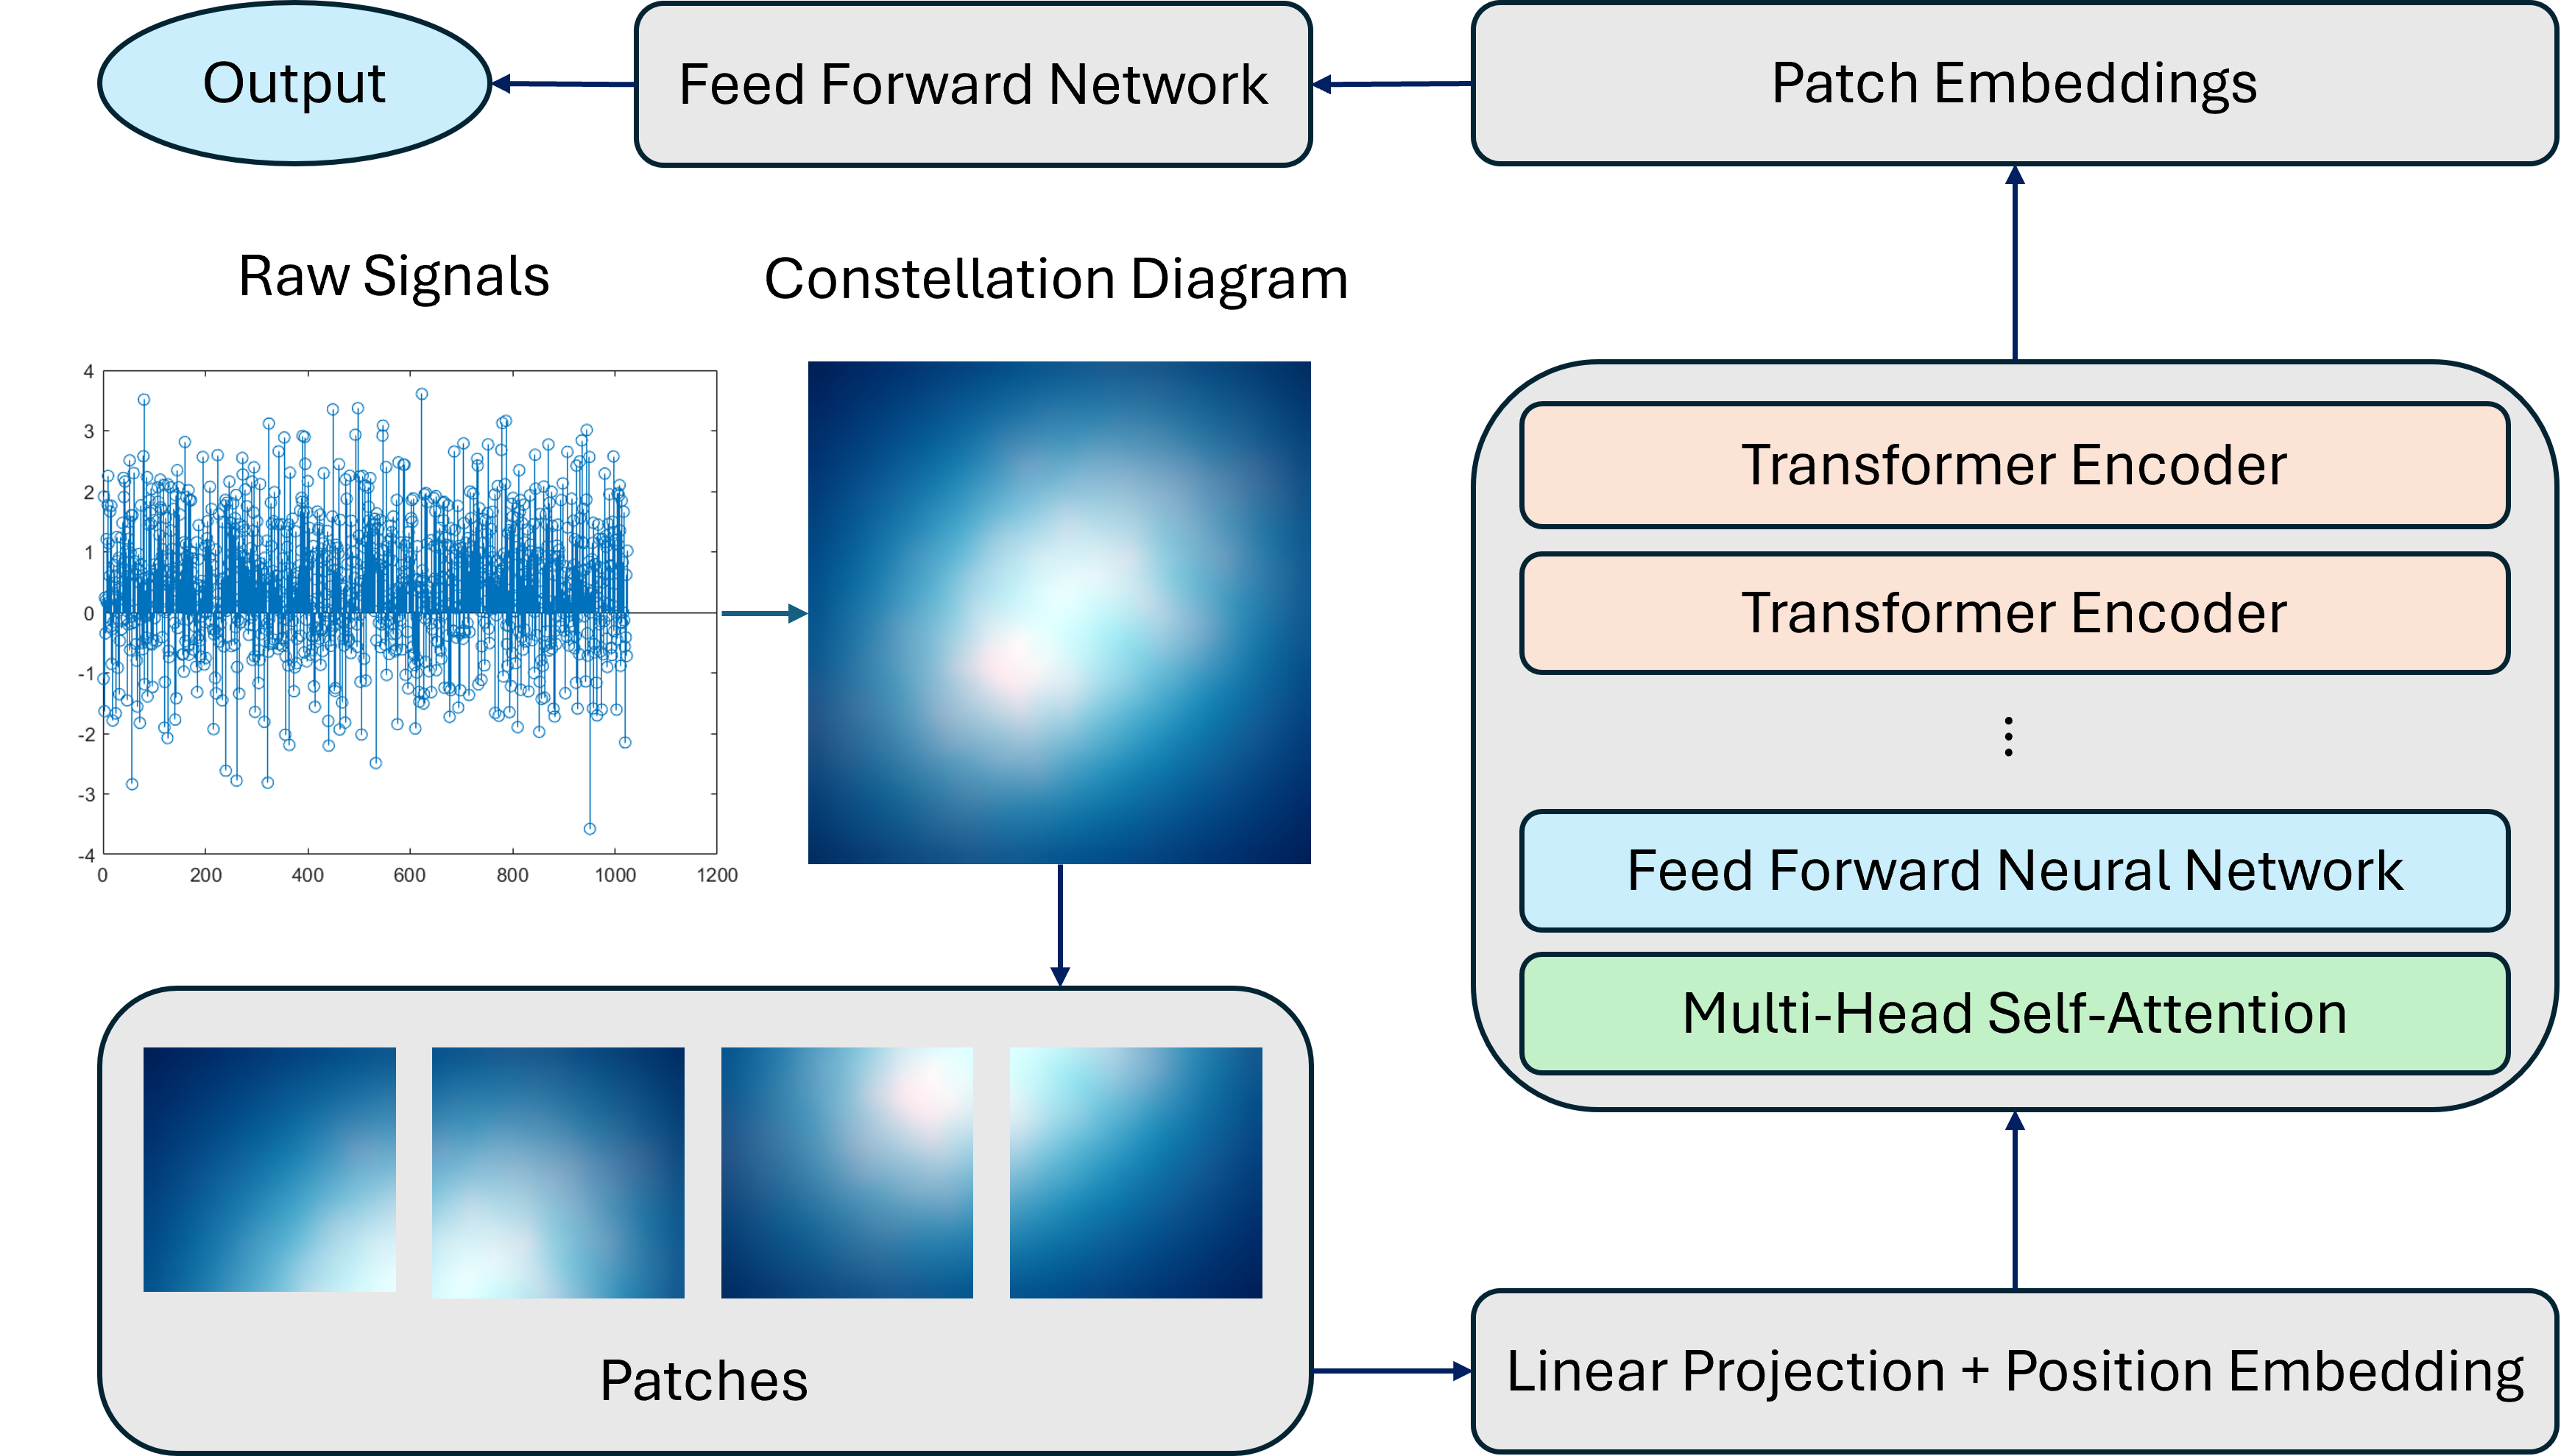
\includegraphics[width=\linewidth]{FIGURES/nmformer/nmformer.png}
    \caption{NMformer system sequential pipeline: starting with generating constellation diagrams from raw signals and culminating in modulation classification using a ViT architecture.}
    \label{fig:trans}
\end{figure} 

\subsubsection{Parameters Selection in Data Generation}

In all our experiments, we explore ten modulation formats. The samples are generated with dimensions of $32$ pixels for both height and width, equating to a sampling frequency of $200$ kHz. The constellation's scale for depiction is fixed at $2.5$. Furthermore, we incorporate reduced path delays of $0$, $0.0004$, and $0.0008$ seconds. The number of filter taps employed is $8$.

\subsubsection{Parameters Selection for Classifier}

For the NMformer, we adhere to most of the hyperparameters outlined in \cite{dosovitskiy2020image} for the network architecture. The input image size is configured to $224\times 224$, representing RGB images. Each input image is partitioned into $16$ equal square patches, which, in ViT, are regarded as tokens and processed by the transformer encoder. Each patch undergoes linear projection to the embedding dimension of $768$. The ViT model comprises $12$ transformer layers. The multi-head self-attention mechanism employs $12$ attention heads, facilitating simultaneous focus on different input segments. The dimensionality of the hidden layers within the feedforward networks in the transformer blocks is fixed at $3,072$.

The number of output classes is set to $10$ for the classification task, aligning with the ten modulation formats. We employ cross-entropy loss and an Adam optimizer with a learning rate $0.00005$. A consistent batch size of $128$ is utilized across all classifiers. The base classifier undergoes training for $50$ epochs, whereas the fine-tuned classifier is trained for $100$ epochs. We implement model saving based on the criterion of achieving the lowest validation loss or the highest validation accuracy, satisfying either condition.

\subsubsection{Base Classifier}

For the base classifier, we consider $11$ variations of SNRs ranging from $0$ dB to $10$ dB. Within each SNR, every training class comprises at least $1,000$ images and up to $1,100$ images. Hence, the total number of training samples amounts to $106,800$. We ensure that the validation set is generated with the same distribution as the training set, which contains samples from SNRs observed during training. Specifically, we generate samples with $4$ different SNRs for validation: $0$ dB, $4$ dB, and $8$ dB, with a total of $3,000$ samples.

During testing, we evaluate the classifier on two distinct datasets: one follows the in-sample distribution, where the data originates from the same SNRs seen during training, while the other is out-of-sample distribution data, comprising novel SNRs not encountered during training.

\subsubsection{Fine-tuned Classifier}

To refine the performance of the base classifier model for specific tasks with limited samples, we engage in fine-tuning the learned parameters. In this process, we freeze all layers of the NMformer except for the last linear layer. During fine-tuning, each SNR is associated with $100$ training samples for each class, contrasting with the base classifier, which has a minimum of $1,000$ samples per class. Post-fine-tuning, we evaluate the model's performance not only on novel classes but also on novel SNRs for both the base and fine-tuned classifiers. 

\subsection{Results and Discussion}

This section presents the test results derived from the base classifier trained over $100$ epochs. However, it is noteworthy that the model attains its optimal performance around the $40^{\mathrm{th}}$ epoch. Therefore, we save the model at this stage and evaluate its performance using the saved parameters. In our experiments, the out-of-distribution data typically presents a more challenging scenario for the classifier than the in-sample distribution. The outcomes are summarized in Table \ref{table:main}.

\begin{table}[htbp]
    \caption{Performance of the classifier on different settings.}
    \label{table:main}
    \centering
    \begin{tblr}{
      colspec={l l c c c c},
      hlines,
      vlines,
      cell{1}{1} = {c=2}{c},
      cell{1}{3} = {c=2}{c},
      cell{1}{5} = {c=2}{c},
      cell{2}{1} = {c=2}{c},
      cell{2}{3} = {c=2}{c},
      cell{2}{5} = {c=2}{c},
      cell{3}{1} = {c=2}{c},
      cell{3}{3} = {c=2}{c},
      cell{3}{5} = {c=2}{c},
      cell{5}{1} = {r=3}{c},
    }
    Model &               & Base           &             & Fine-tuned     &             \\
    Sample &             & 106{,}800      &             & 3{,}000        &             \\
    ~      &             & Accuracy (\%)  &             & Accuracy (\%) &             \\
    Distribution Type &  SNRs            & In          & Out            & In          & Out         \\
                     & 0 dB, 4 dB, 10 dB & 71.10       & -              & -           & -           \\
                     & 0.5, 1.5, 4.5 dB  & -           & 67.48          & 71.60       & 70.51       \\
                     & 5.5, 7.5, 9.5 dB  & -           & 72.12          & 75.77       & 71.87       \\
    \end{tblr}
    \end{table}


In the first test, we evaluated the performance of the base classifier using data from the same distribution. Specifically, the test classes included SNRs of $0$ dB, $4$ dB, and $10$ dB. The resulting test accuracy achieved in this scenario was \(71.10\%\).

Subsequently, we conducted tests on two out-of-distribution datasets. The first dataset comprises SNRs of $0.5$ dB, $1.5$ dB, and $4.5$ dB, where the lower SNRs pose greater challenges for classification. In this case, the obtained test accuracy is \(67.48\%\). Conversely, the second dataset contains SNRs of $5.5$ dB, $7.5$ dB, and $9.5$ dB, presenting less challenging classification tasks due to higher SNRs. Here, we achieved a test accuracy of \(72.12\%\).

The challenges posed by different SNR distributions are reflected in the accuracy results, where the less challenging distribution yields higher accuracy than the base classifier tested on all the in-distribution samples.

In the subsequent task, we fine-tune the base classifier using only a limited number of samples for specific SNRs. For the in-distribution SNRs of $0.5$ dB, $1.5$ dB, and $4.5$ dB, we achieve an accuracy of \(71.60\%\). Surprisingly, this surpasses the accuracy of the base classifier by \(0.50\%\), despite the samples having lower SNRs. This result demonstrates that our model can achieve higher accuracy when fine-tuned with a few yet challenging samples.

Conversely, when tested with higher SNR samples of $5.5$ dB, $7.5$ dB, and $9.5$ dB, the same fine-tuned classifier achieves an accuracy of \(71.87\%\). This accuracy is higher than that of the in-distribution samples, as higher SNR samples are less challenging to classify.

Furthermore, our test on the in-distribution samples of $5.5$ dB, $7.5$ dB, and $9.5$ dB yields the highest accuracy of all, \(75.77\%\). On the other hand, the out-of-distribution samples with SNRs of $0.5$ dB, $1.5$ dB, and $4.5$ dB achieve the lowest accuracy, which is \(70.51\%\). This lower accuracy is expected since the classifier is trained on fewer noisy samples, performing better on similar samples but experiencing a drop in accuracy for noisier ones. Nevertheless, this accuracy is \(3.03\%\) higher than that of our base classifier for the same distribution, demonstrating the superiority of our fine-tuned classifier.

We present the model convergence plots illustrating the smooth convergence of our fine-tuned model. These plots showcase the convergence behavior across different SNRs, specifically at $0.5$ dB, $1.5$ dB, and $4.5$ dB for the more challenging tasks and at $5.5$ dB, $7.5$ dB, and $9.5$ dB for the less challenging tasks.

Although the training and validation losses closely align in the first plot, they are noticeably higher compared to the latter plot. Consequently, the model achieves relatively lower accuracy at lower SNRs. However, across both plots, the model consistently converges towards the global minima as the training progresses.

\begin{figure}[htbp]
    \centering
    \begin{subfigure}[b]{0.48\textwidth}
        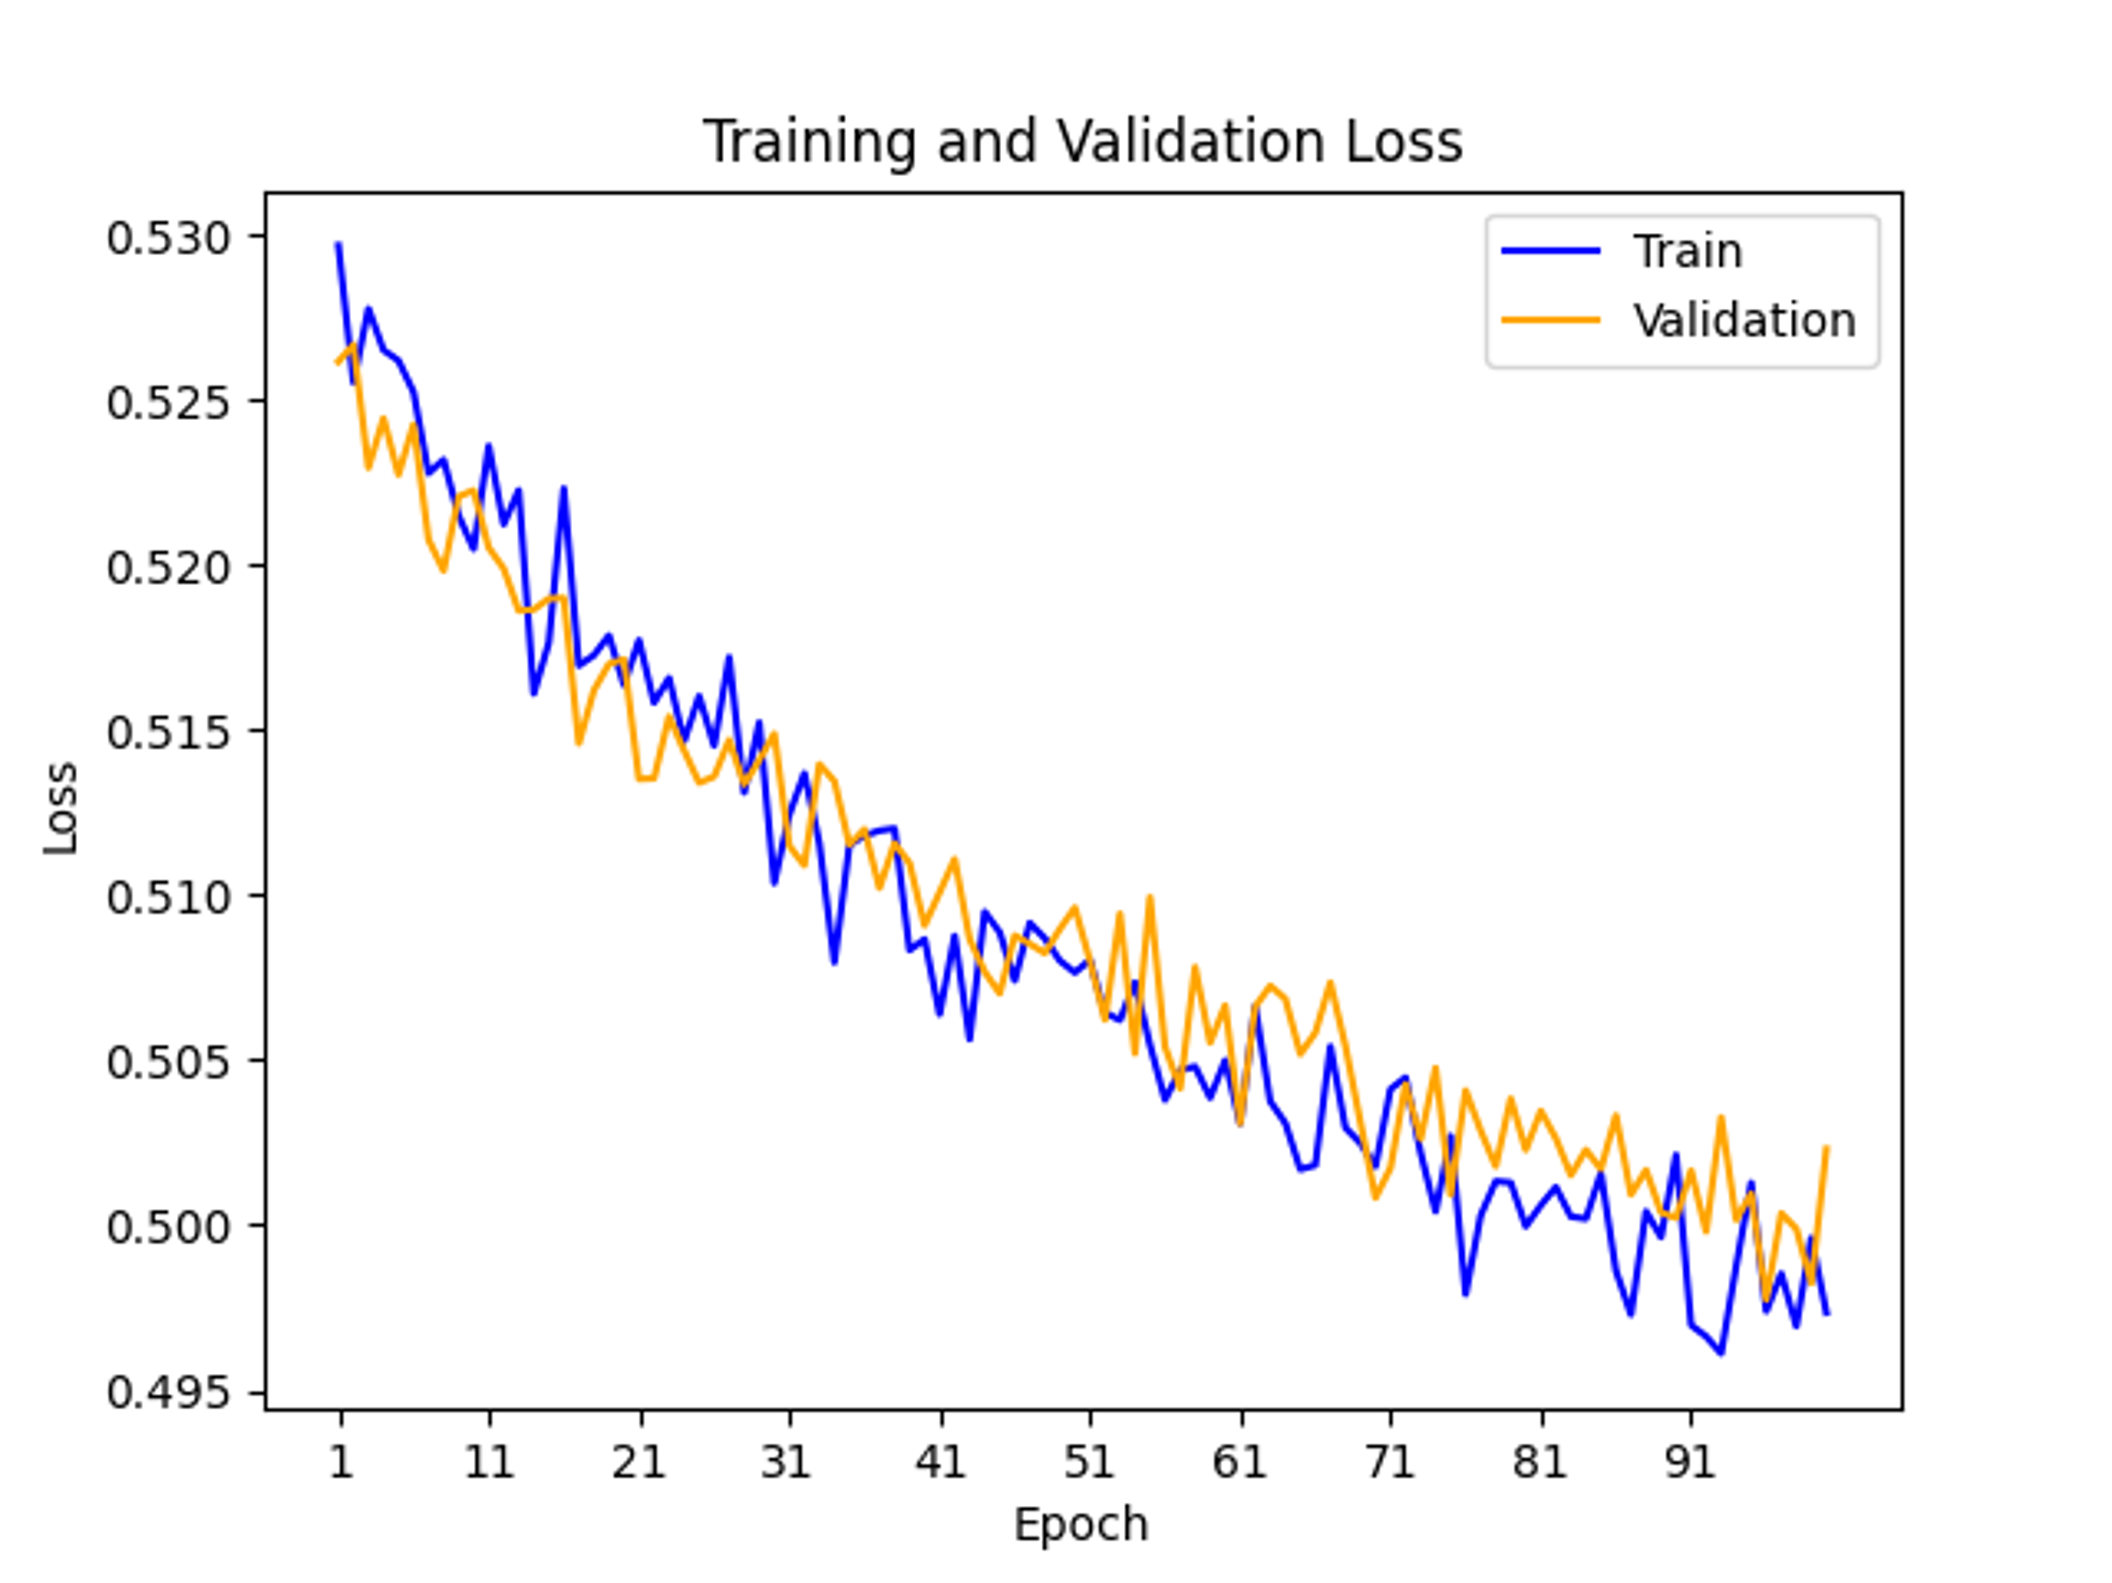
\includegraphics[width=\textwidth]{FIGURES/nmformer/loss_plot_l.png}
        \caption{Loss for 0.5 dB, 1.5 dB, and 4.5 dB SNRs.}
        \label{fig:sub1}
    \end{subfigure}
    \hspace{0.02\textwidth}
    \begin{subfigure}[b]{0.48\textwidth}
        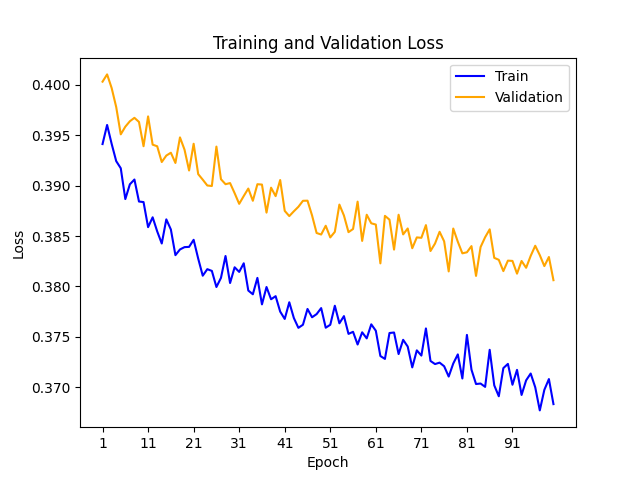
\includegraphics[width=\textwidth]{FIGURES/nmformer/loss_plot_h.png}
        \caption{Loss for 5.5 dB, 7.5 dB, and 9.5 dB SNRs.}
        \label{fig:sub2}
    \end{subfigure}
    \caption{Loss convergence plots across different SNR settings.}
    \label{fig:main}
\end{figure}

In Figure \ref{fig:conf}, we present the confusion matrices for our base classifier and two fine-tuned classifiers. Notably, all samples were misclassified for classes OOK and 16PAM in the base classifier. However, in Figure \ref{fig:conf}(b), corresponding to the fine-tuned classifier, we observe a notable increase in correctly classified samples for these classes. Subsequently, in Figure \ref{fig:conf}(c), there is a significant further increase in the number of correctly classified samples, indicating the clear superiority of our fine-tuned classifier.

To dive deeper into class performance analysis, we compute the classifier's precision, recall, and F1 score, as shown in Table \ref{table:pre}. The base classifier exhibits the lowest precision, recall, and F1 score among all classifiers. The precision, recall and F1 score values show improvement for both the fine-tuned classifiers. Notably, the fine-tuned classifier with a higher SNR achieves the highest F1 score, indicating superior performance across all evaluated metrics.

\begin{figure}[!htbp]
  \centering
  \begin{subfigure}[b]{0.55\textwidth}
    \centering
    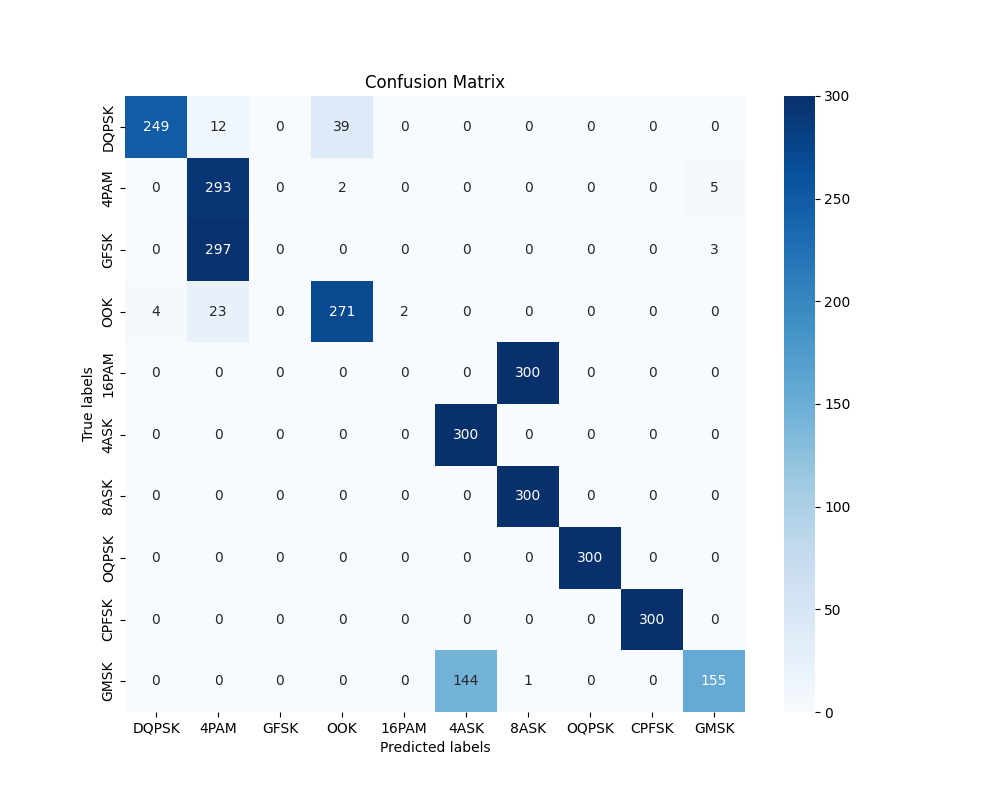
\includegraphics[width=0.7\textwidth]{FIGURES/nmformer/vit1_con.png}
    \caption{Base classifier.}
    \label{fig:subplot1}
  \end{subfigure}
  \begin{subfigure}[b]{0.55\textwidth}
    \centering
    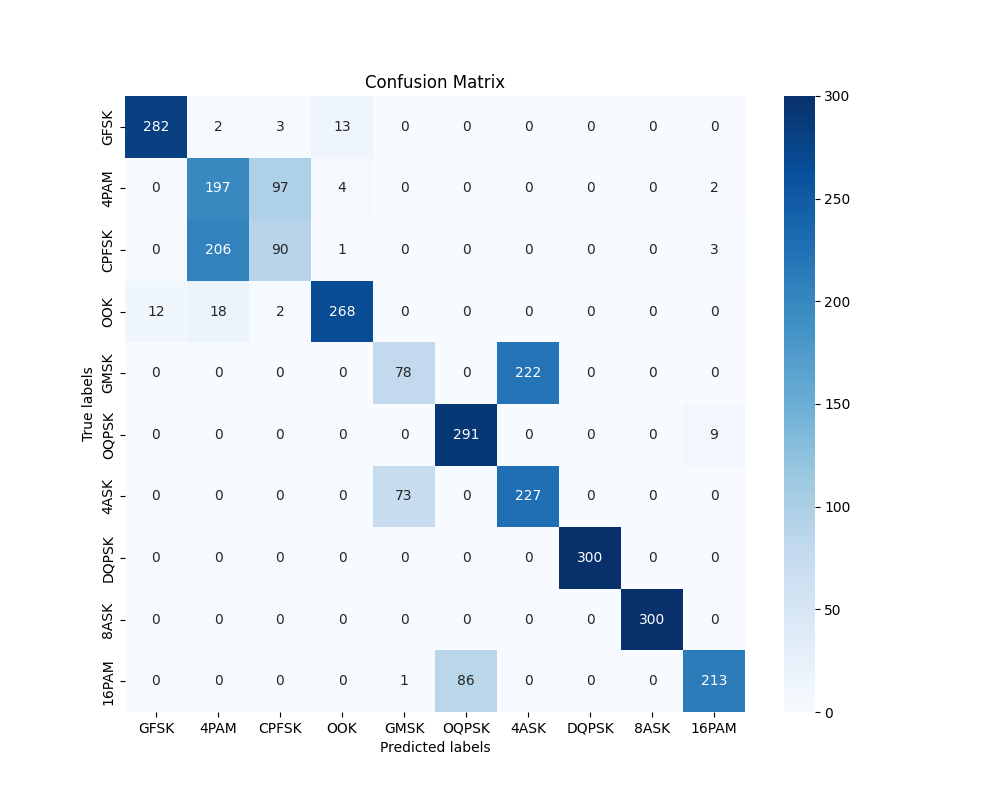
\includegraphics[width=0.7\textwidth]{FIGURES/nmformer/vit_f_p_con.png}
    \caption{Fine-tuned (0.5 dB, 1.5 dB, 4.5 dB).}
    \label{fig:subplot2}
  \end{subfigure}
  \begin{subfigure}[b]{0.55\textwidth}
    \centering
    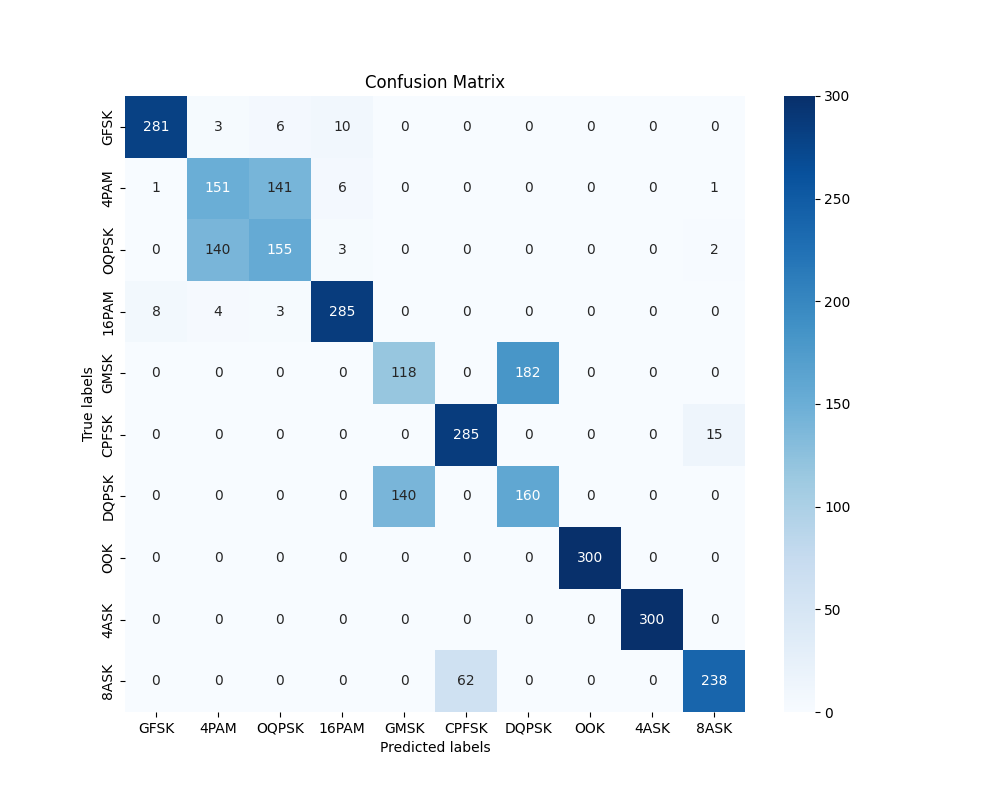
\includegraphics[width=0.7\textwidth]{FIGURES/nmformer/vit_f_p_h_con.png}
    \caption{Fine-tuned (5.5 dB, 7.5 dB and 9.5 dB).}
    \label{fig:subplot3}
  \end{subfigure}
  \caption{Confusion matrix for different classifiers.}
  \label{fig:conf}
\end{figure}

\begin{table}[htbp]
\caption{Analysis of classifier performance.}
\centering
\begin{tabular}{llll}
\hline
Classifier                             & Precision & Recall  & F1 Score \\
\hline
Base (0 dB – 10 dB)                    & 0.6170    & 0.6933 & 0.6291   \\
Fine-tuned (0.5 dB, 1.5 dB, 4.5 dB) & 0.7188    & 0.7163 & 0.7118   \\
Fine-tuned (5.5 dB, 7.5 dB, 9.5 dB) & 0.7598    & 0.7577 & 0.7572  \\
\hline
\end{tabular}
\label{table:pre}
\end{table}

\subsection{Conclusion}

In this study, we presented an effective model named NMformer for modulation classification in wireless communication systems leveraging a ViT model. Our proposed AMC method achieves remarkable accuracy across diverse SNRs by training on constellation diagrams of modulation signals. We demonstrate substantial improvement in classification performance by carefully fine-tuning the base classifier with limited samples tailored to specific SNRs. Our method surpasses the baseline classifier's accuracy and exhibits superior resilience to out-of-distribution data, particularly in challenging low SNR scenarios. The efficacy of our approach is further underscored by the precision, recall, and F1 score analyses, which consistently show significant improvements in classification metrics, particularly for classes traditionally prone to misclassification. Overall, our findings underscore the potentiality of NMformer for classifying noisy modulation signals.

\section{Task 2: DenoMAE: A Denoising Masked Autoencoder for Modulation Classification}

\subsection{Introduction}

Recent deep learning approaches have shifted toward addressing the high costs and scarcity of labeled data. Self-supervised learning has emerged as an efficient solution that leverages abundant raw data during pretraining, drastically reducing labeled data requirements while maintaining strong downstream performance \cite{balestriero2023cookbookselfsupervisedlearning}. These methods have shown remarkable success in natural language processing \cite{roberts2019exploring}, computer vision \cite{caron2021emerging} and other domains, opening new applications in fields with limited labeled data, including communications.

Wireless communication systems face critical challenges in maintaining reliable signal classification and interpretation, particularly in dynamic and noise-laden environments. Current approaches to modulation signal classification are predominantly supervised, requiring substantial amounts of labeled data across various Signal-to-Noise Ratios (SNRs) to achieve acceptable performance \cite{zheng2024deep}. These models often exhibit significant degradation when faced with previously unseen modulation types or noise conditions that deviate from their training distribution \cite{9965389}. This performance gap is striking in low SNR scenarios, where noise dominates the signal characteristics, leading to misclassifications and system failures \cite{perenda2021learning}. Despite advances in deep learning architectures for communications, the fundamental challenge remains: developing models that simultaneously maintain robustness to noise variation and generalize effectively with minimal labeled data requirements.

Existing solutions have explored several directions to address these challenges. Traditional denoising techniques treat noise as an unwanted component to be filtered out, often leading to information loss in the original signal \cite{shi2023gaf}. Single-modality masking approaches have shown promise in learning representations but fail to capture the complex interplay between signal characteristics and noise patterns. More recent multimodal learning approaches \cite{bachmann2022multimae, bachmann20244m} integrate data from multiple sources but typically treat noise as a distortion rather than an informative signal component. This fundamental limitation prevents these models from fully understanding the structural relationship between noise and signal modalities, restricting their ability to generalize across varying noise conditions. Additionally, most current methods require extensive labeled datasets across multiple SNR levels, making them impractical for rapidly evolving communication environments.

Our motivation stems from a key insight: noise in communication signals contains valuable structural information that enhances representation learning. By treating noise as an additional modality rather than a nuisance, we develop models that learn intrinsic relationships between clean signals and their noisy counterparts, enabling better generalization with less data. Building on this, we present DenoMAE, a multimodal autoencoder designed for communication systems that treats noise as an additional modality. This approach allows the model to generate all modalities from a single input, helping it comprehensively understand noise across modalities while enhancing denoising capabilities and learning robust signal representations. We employ random masking to challenge the model in reconstructing missing patches, reducing computational complexity while introducing beneficial uncertainty for effective learning.

\begin{figure}[htbp]
    \centering
    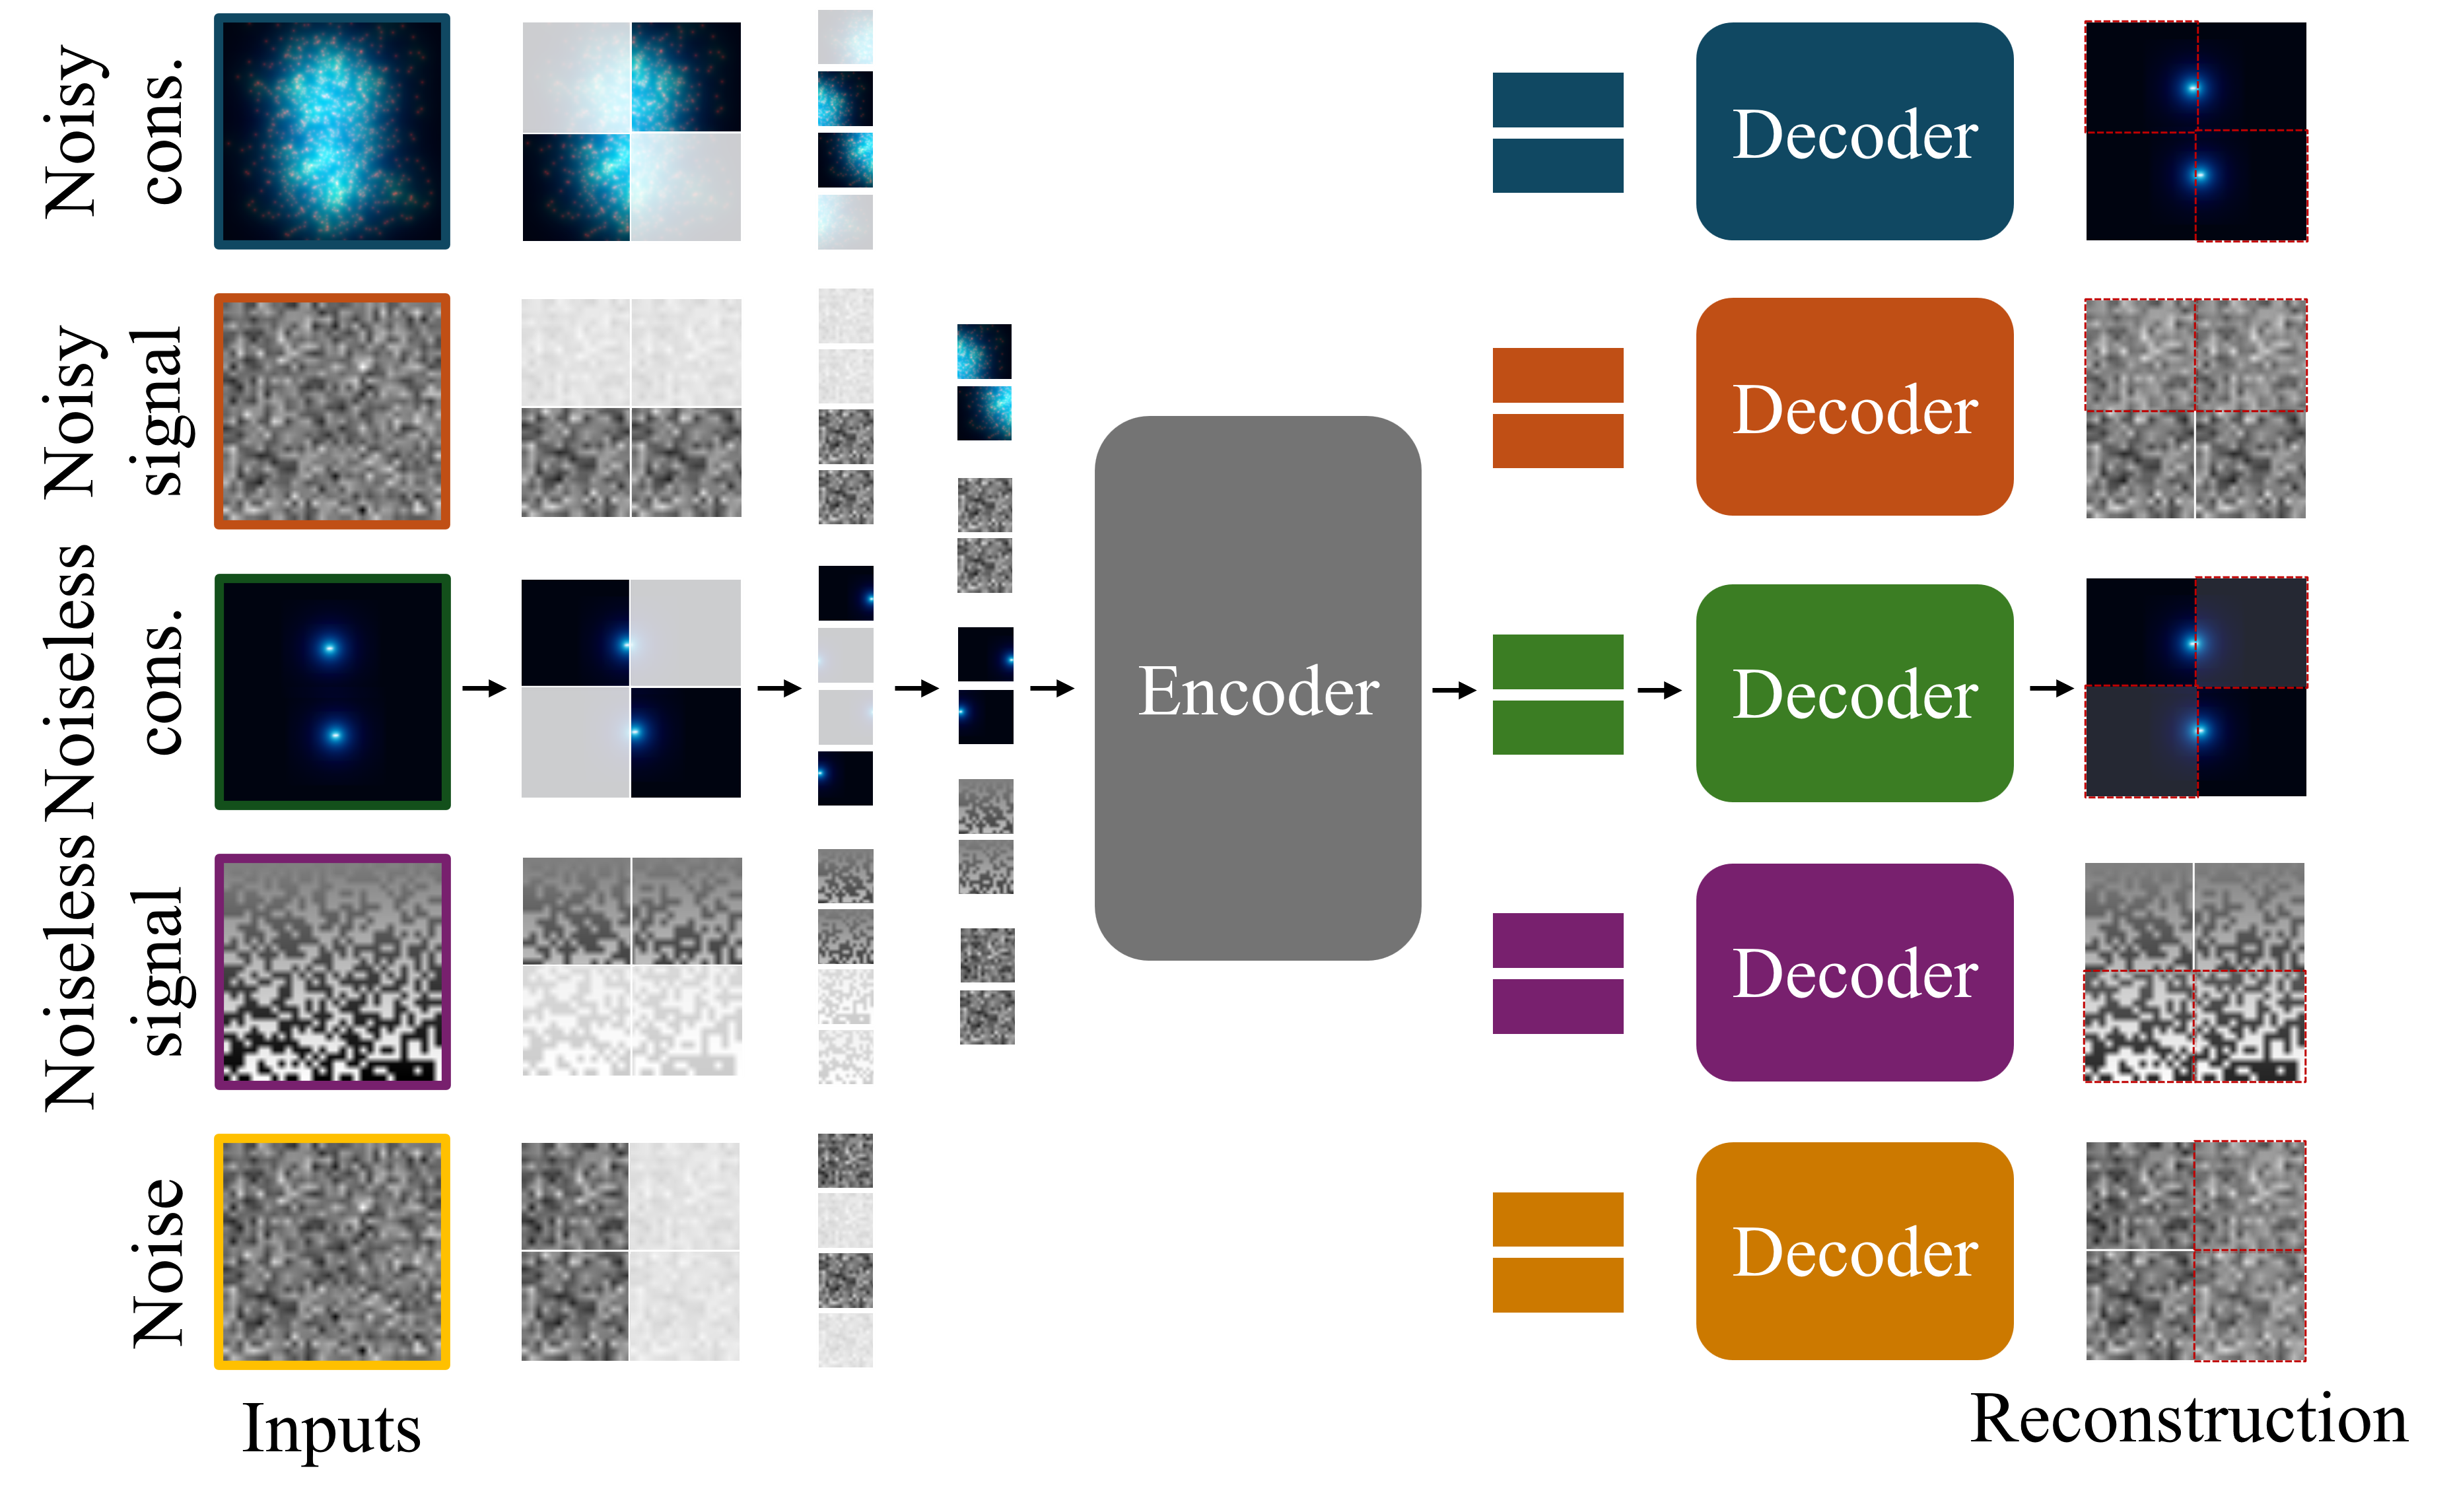
\includegraphics[width=\linewidth]{FIGURES/denomae/fig_new.png} % Adjust width as needed
    \caption{
    \textbf{DenoMAE Pretraining Strategy}: We apply a random 75\% masking \cite{he2022masked} (not to scale in the illustration) across all input modalities. The remaining 25\% of visible patches are processed by a shared encoder, while each modality utilizes a dedicated decoder to reconstruct its masked patches. Only the encoder is reused for fine-tuning the downstream tasks.
    }
    \label{fig:architecture} 
\end{figure}

\subsection{Contributtions}

Our contributions to DenoMAE are threefold:

\begin{itemize} 
\item We propose a novel multimodal paradigm that incorporates noise as an additional modality, enabling more effective pretraining on modulation signals and enhancing model resilience to noise. 
\item We demonstrate that our pre-trained model achieves significant improvements in classification accuracy under low SNR conditions, with accuracy gains of up to 22.1\% over non-pre-trained models. 
\item DenoMAE outperforms traditional methods, achieving superior results while requiring only one-tenth of the unlabeled data for pretraining and one-third of the labeled data for fine-tuning, underscoring its efficiency and scalability for real-world applications. 
\end{itemize}

\subsection{Related Work}

\textbf{Modulation Classification}: Recent advancements in deep learning have transformed AMC by enabling advanced analysis of constellation and other image diagrams. Much of the research emphasizes CNN-based architectures designed to classify modulation types while handling varying channel conditions \cite{huynh2020mcnet}. Innovative approaches include time-frequency adaptive decomposition with hybrid neural networks that reduce model parameters while maintaining accuracy and interpretability \cite{10945334}. Attention-based models like LSTMs and GRUs have evolved for processing modulation signals as time-series data \cite{8446021, liu2021automatic}, with transformer-based architectures gaining prominence for their ability to incorporate global sequence information \cite{kong2023transformer}. Transformer-deep recurrent hybrids have shown particular promises \cite{10668824}, while contrastive learning approaches have emerged to address generalization error and improve transferability under low SNR conditions \cite{10857965}. Recent semi-supervised frameworks combine transformers with contrastive learning to overcome labeled data limitations \cite{10093837}. Despite these advancements, many architectures still lack robustness across diverse noise scenarios, limiting their generalization beyond specific tasks.

\textbf{Multisensory Masked Modeling}: Masking large portions of the input and training the model to reconstruct or predict missing elements has become a popular self-supervised approach, especially within autoencoder-based methods. For example, BERT \cite{devlin2018bert} introduced masked language modeling by masking words in sentences and training the model to predict them, a concept adapted for vision with Masked Autoencoders (MAE) \cite{he2022masked}, where image patches are masked to encourage the model to learn robust visual representations. In multimodal contexts, masked modeling extends to tasks combining text, vision, and audio, promoting cross-modal understanding. For instance, Vision-Language Pretraining (VLP) models \cite{wang2022image} utilize masked language and vision modeling to jointly learn from masked image regions and text tokens. Additionally, image modality-centered models like MultiMAE \cite{bachmann2022multimae} and 4M \cite{mizrahi20244m} have demonstrated strong performance by pretraining on multiple image modalities and enhancing inference capabilities across diverse inputs. These multimodal masking methods have demonstrated significant gains in self-supervised learning, advancing model performance in tasks that benefit from multimodal reasoning.

\subsection{DenoMAE Architecture}

DenoMAE consists of four primary components: input embedding, encoder, shared latent space, and decoder. Figure \ref{fig:architecture} illustrates the overall architecture. Our codes are public at \url{https://github.com/atik666/denoMae/tree/master}.

\subsubsection{Input Embedding}

For each modality $m \in {1, ..., n}$, we represent the input as a $C$-channel image $X_m \in \mathbb{R}^{C \times H \times W}$. We divide each image into non-overlapping patches of size $p \times p$, resulting in $N = (H/p)^2$ patches per modality. Each patch is flattened and linearly projected to a $D$-dimensional embedding space:

\begin{equation}
E_m = [e^m_1, ..., e^m_N] + E_{pos}, \quad e^m_i \in \mathbb{R}^D
\end{equation}

where $E_{pos}$ represents learnable positional embeddings. Here, $e^m_i$ denotes the $i$-th patch embedding for modality $m$, and $N$ is the total number of patches per modality.

\subsubsection{Encoder}

The encoder $f_{\textrm{enc}}$ is a series of $L$ transformer blocks. We randomly mask a high proportion (e.g., 75\%) of the input patches for each modality. The encoder processes the visible patches:

\begin{equation}
H_m = f_{\textrm{enc}}([e^m_{i_1}, ..., e^m_{i_k}]), \quad i_j \in \text{visible patches}
\end{equation}

\subsubsection{Shared Latent Space}

To enable cross-modal learning, we project the encoded representations from all modalities into a shared latent space. We use a linear projection followed by layer normalization, $LN$:

\begin{equation}
Z_m = LN(W_m H_m + b_m)
\end{equation}

where $W_m$ is the projection matrix for modality $m$, $H_m$ is the encoded representation, and $b_m$ is the corresponding bias term.

The shared latent representation $Z_m$ is the concatenation of all modality-specific projections:
$Z_m = [Z_1; ...; Z_n]$.

\subsubsection{Decoder}

The decoder $f_{\textrm{dec}}$ reconstructs the masked patches for all modalities simultaneously. It takes the shared latent representation $Z_m$ as input and processes it through a series of transformer blocks. The output is then split into modality-specific representations and projected back to the original patch space:

\begin{equation}
\hat{X}_m = f_{\textrm{proj}_m}(f_{\textrm{dec}}(Z_m))
\end{equation}

where $f_{\textrm{proj}_m}$ is a modality-specific projection layer.

\subsubsection{Loss Function}

We employ a multi-modal reconstruction loss that combines individual losses for each modality:

\begin{equation}
\mathcal{L} = \sum_{m=1}^n w_m \mathcal{L}_m
\end{equation}

where $w_m$ is the weight for modality $m$, and $\mathcal{L}_m$ is the reconstruction loss for that modality. We use the Mean Squared Error (MSE) as the reconstruction loss.

\subsection{Fine-Tuning on Downstream Tasks}

After pretraining, we adapt the encoder for downstream tasks by removing the decoder and attaching a classification head. For modulation classification, we use a two-layer multi-layer perceptron network (MLP) with ReLU activation and dropout regularization. The process begins by embedding input patches and adding positional embeddings to form $x'$. The encoder processes these embeddings, and we apply global average pooling (GAP) to obtain representation $z$. This representation passes through the classifier to produce predictions $\hat{y}$:

\begin{equation}
\hat{y} = W_2(ReLU(W_1 \cdot GAP(f_{enc}(x')) + b_1)) + b_2
\end{equation}

During fine-tuning, we optimize the entire network using cross-entropy loss, with the pretrained encoder parameters updated at a reduced learning rate. 

\subsection{Experimental Setup}

To evaluate the effectiveness of DenoMAE in modulation classification tasks, we conducted a series of experiments under varying signal-to-noise ratio (SNR) conditions. Our experimental methodology encompasses data preparation, model architecture configuration, pretraining strategy, and fine-tuning protocols.

\subsubsection{Constellation Diagram Generation}

Constellation diagrams provide more informative visualization for modulation classification than raw signals \cite{doan2020learning}. The generation process involves mapping signals onto a complex plane across SNR ranges of $-10$ dB to $10$ dB. Our enhancement process involves two steps: creating a gray image that handles varying pixel densities, then developing enhanced grayscale images using an exponential decay model that accounts for sample positions and neighborhood influence. This model incorporates sample power, point-pixel distance, and decay rate parameters. For compatibility with DenoMAE's RGB input requirements, we generate three-channel images by creating distinct enhanced grayscale images from the same data samples, each with different exponential decay rates.

\subsubsection{Parameters in Sample Generation} 

The dataset comprises signals from ten modulation formats, each originally of length $L_0 = 1024$. To conform to the transformer's input dimensions, signals undergo a two-step preprocessing: (1) reshaping to $\mathbf{S}_1 \in \mathbb{R}^{32 \times 32}$, and (2) interpolation to $\mathbf{S}_2 \in \mathbb{R}^{224 \times 224}$. For formats with $L_0 > 1024$ (e.g., $L_\text{GMSK} = 8196$), signals are initially downsampled to $L_0$. To match the three-channel structure of constellation images $\mathbf{I} \in \mathbb{R}^{3 \times 224 \times 224}$, $\mathbf{S}_2$ is replicated across three channels, yielding $\mathbf{S}_3 \in \mathbb{R}^{3 \times 224 \times 224}$. All signals are sampled at $f_s = 200$ kHz, ensuring consistency across modulation formats.

\subsubsection{Parameters for DenoMAE}

The DenoMAE architecture processes $n=5$ modalities of input images $\mathbf{X} \in \mathbb{R}^{3 \times 224 \times 224}$, segmented into $16 \times 16$ patches. The model employs a transformer-based encoder-decoder structure with $d_\text{model} = 768$ embedding dimensions. The encoder consists of $L_e = 12$ layers, while the decoder uses $L_d = 4$ layers, both utilizing $h = 12$ attention heads. During training, a random masking strategy with $p_\text{mask} = 0.75$ is applied. The model is optimized using AdamW with learning rate $\eta = 10^{-4}$ over $100$ epochs, using batches of size $B = 64$. This flexible architecture allows for easy adaptation to various multi-modal denoising tasks.

\subsubsection{Finetuning Parameters}

The fine-tuning task adapts the pre-trained DenoMAE model for classification across $C = 10$ classes. The encoder $f_{\textrm{enc}}$ from DenoMAE, with a depth, $d_\text{model} = 768$, is used as a backbone, followed by a classifier head $H(\cdot)$ consisting of a two-layer MLP with hidden dimension 512 and dropout $p = 0.5$, for an input $X \in \mathbb{R}^{3 \times 224 \times 224}$. The model is trained for $N_{\textrm{epoch}} = 150$ epochs using Adam optimizer with learning rate $\eta = 10^{-4}$ and batch size $B = 32$. Training data undergoes normalization but no augmentation.

\subsection{Results and Discussion}

This section presents a comprehensive analysis of DenoMAE's performance across various signal-to-noise ratios and modulation schemes. We examine the model's reconstruction capabilities during pretraining, classification accuracy during fine-tuning, and comparative performance against baseline approaches. Our analysis particularly focuses on the performance improvements in low SNR environments, which represent the most challenging scenarios for modulation classification in real-world applications. Additionally, we investigate the data efficiency of our approach compared to traditional supervised methods.

\begin{figure}[htbp]
    \centering
    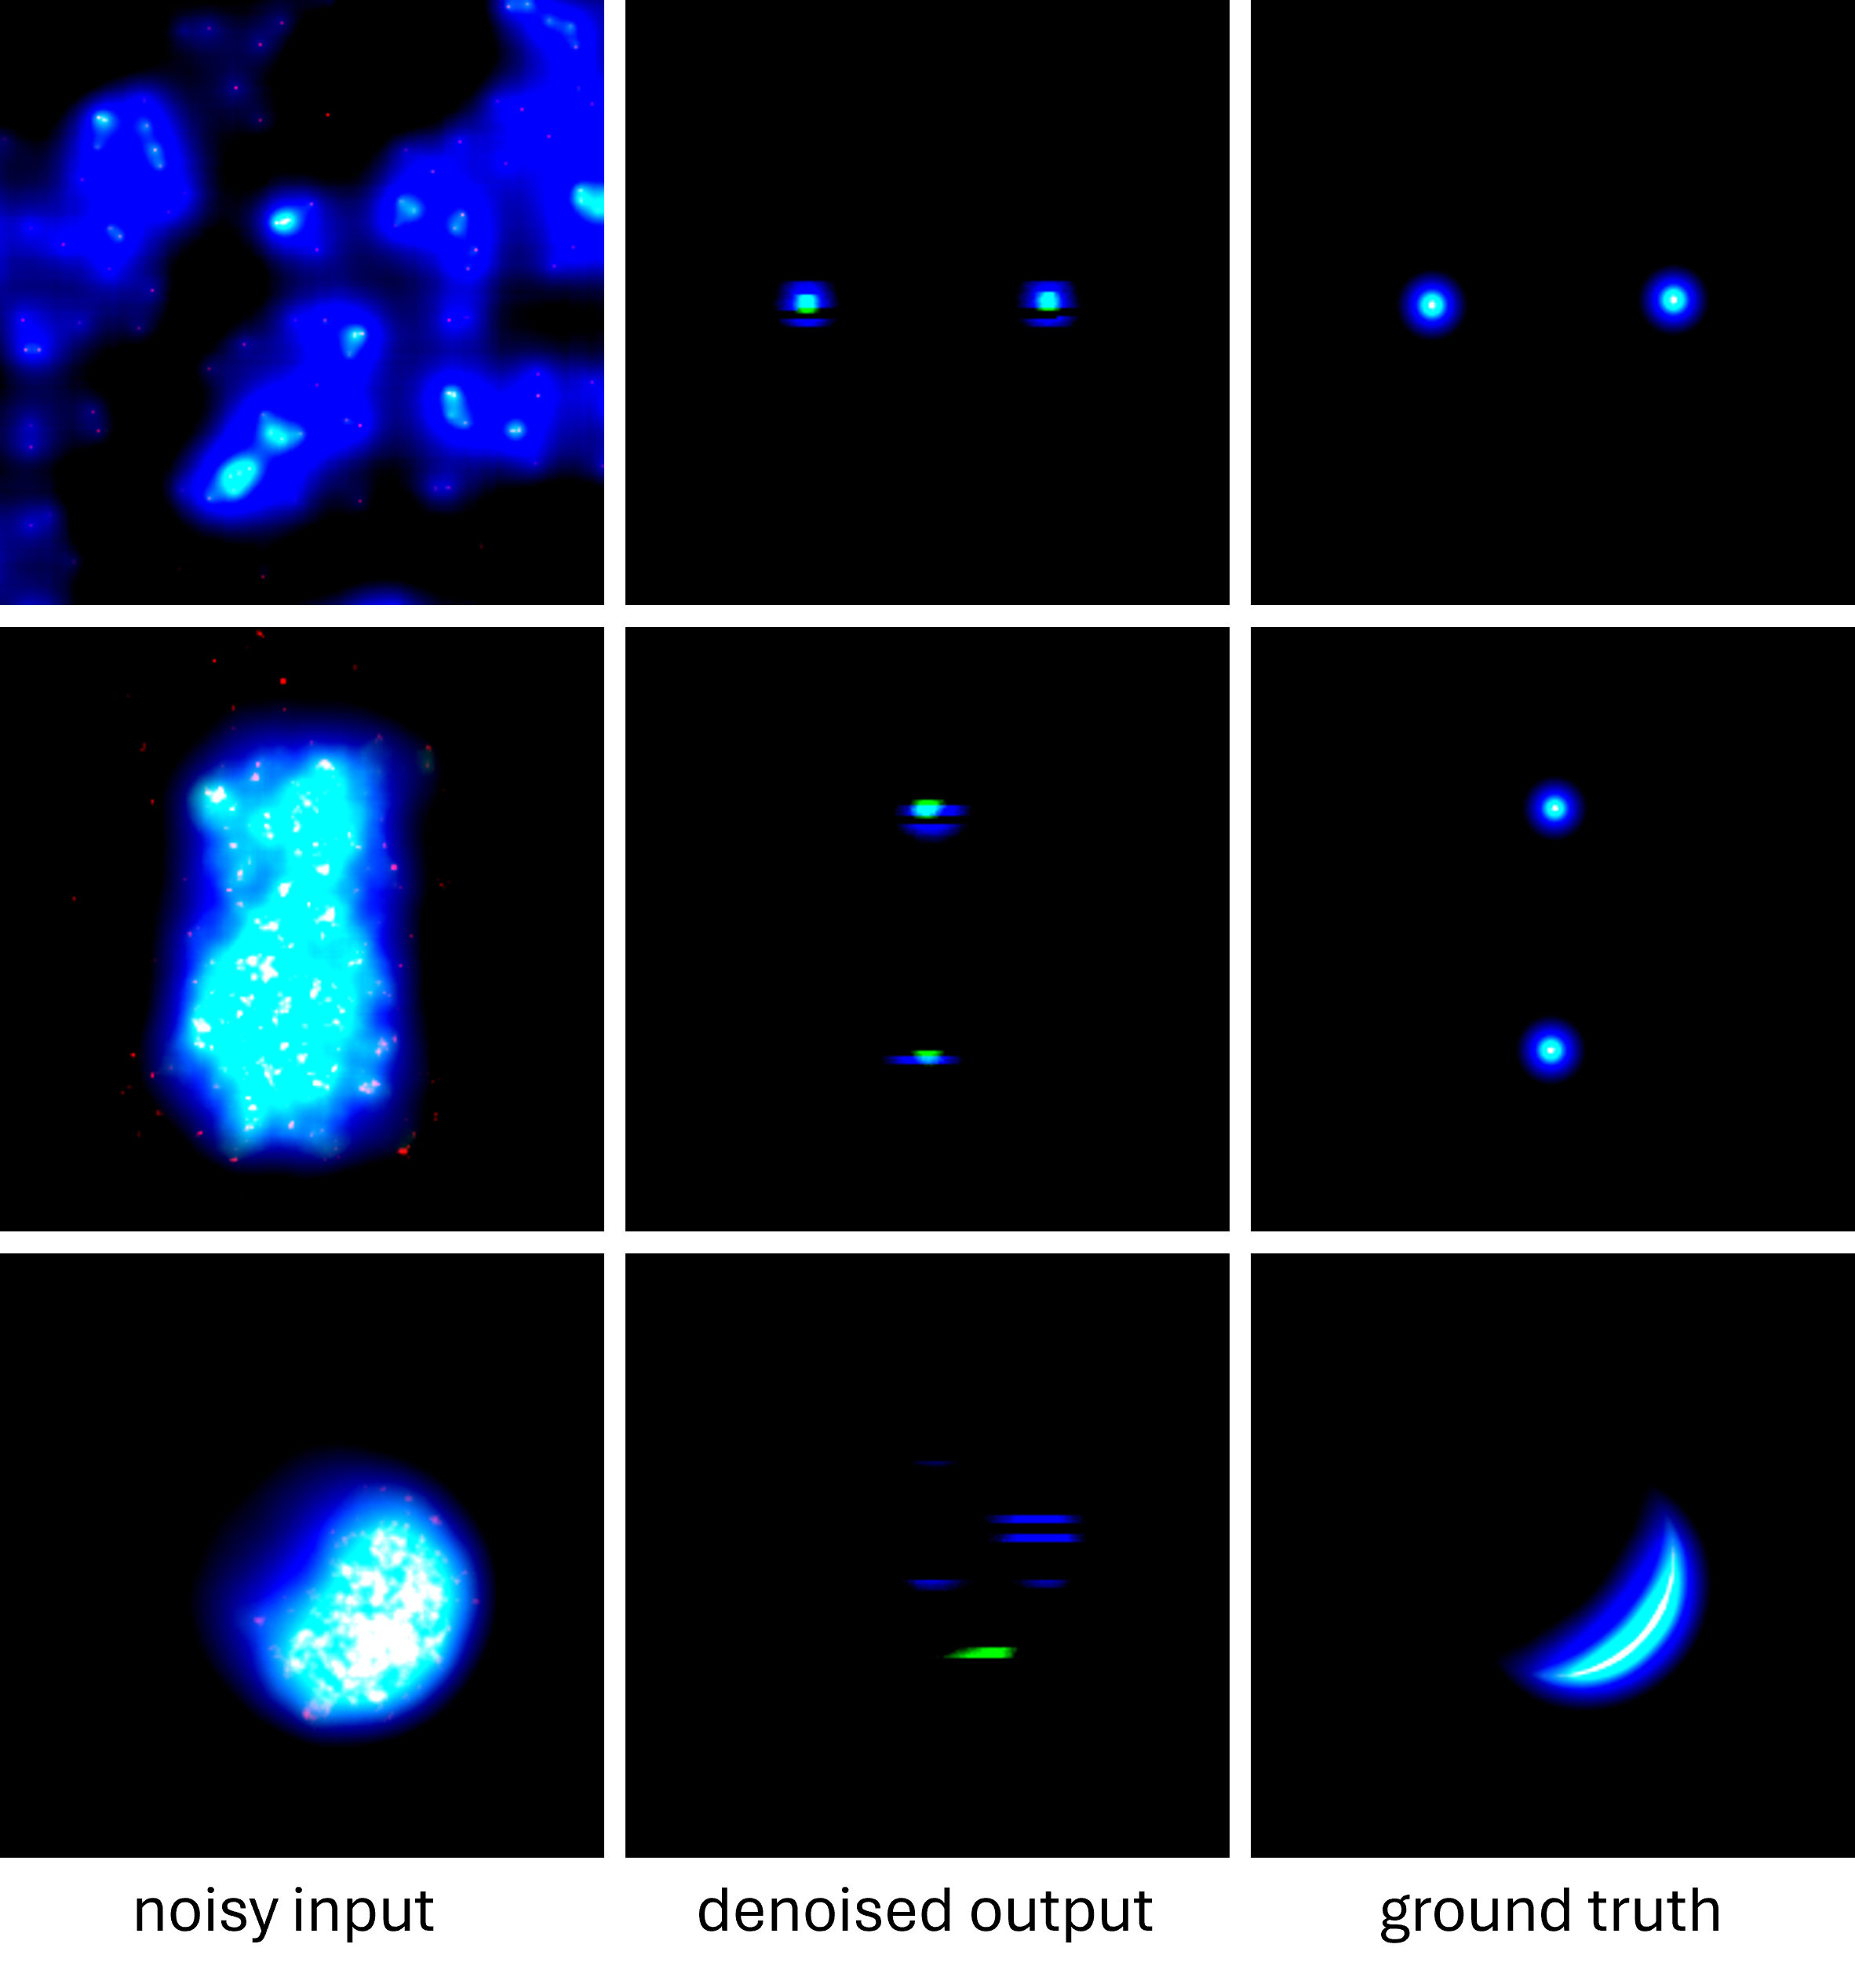
\includegraphics[width=0.75\linewidth]{FIGURES/denomae/outputs.png} 
    \caption{Denoised outputs on constellation diagrams at different SNRs.}
    \label{fig:outputs} % Label for referencing
\end{figure}

\subsubsection{Pretraining Performance}

The pretraining effectiveness of DenoMAE was evaluated using $10,000$ unlabeled signal samples across five modalities. We used 100 constellation samples equally distributed across classes as validation data during pretraining. Visual inspection of the denoised constellation diagram outputs (Figure \ref{fig:outputs}) demonstrates strong reconstruction capabilities, particularly for samples in the first two rows where the model successfully removes noise while preserving signal characteristics. While reconstruction quality slightly diminishes for samples in the last row, the overall shape and pattern retention remain sufficient for downstream tasks.

\subsubsection{Impact of SNRs}

In fine-tuning, we utilized a labeled dataset comprising of constellation images evenly distributed across classes. The dataset was partitioned into $1,000$ training images, $100$ validation images, and $100$ testing images, with 10 classes: 4ASK, 8ASK (Amplitude Shift Keying), 4PAM, 16PAM (Pulse Amplitude Modulation), CPFSK (Continuous Phase Frequency Shift Keying), DQPSK (Differential Quadrature Phase Shift Keying), GFSK (Gaussian Frequency Shift Keying), GMSK (Gaussian Minimum Shift Keying), OOK (On-Off Keying), OQPSK (Offset Quadrature Phase Shift Keying). The impact of SNR on classification performance reveals DenoMAE's robust noise resilience. As shown in Figure \ref{accuracy}, the pre-trained model achieves 77.50\% accuracy even at $-10$ dB SNR, with performance steadily improving to 84.30\% at $10$ dB. The pretraining advantage is most pronounced in challenging low-SNR conditions, demonstrating a 22.1\% improvement over the non-pre-trained baseline at $-10$ dB. This performance gap gradually narrows at higher SNRs, suggesting that pretraining is particularly valuable for learning noise-robust features.

\begin{figure}[htbp]
    \centering
    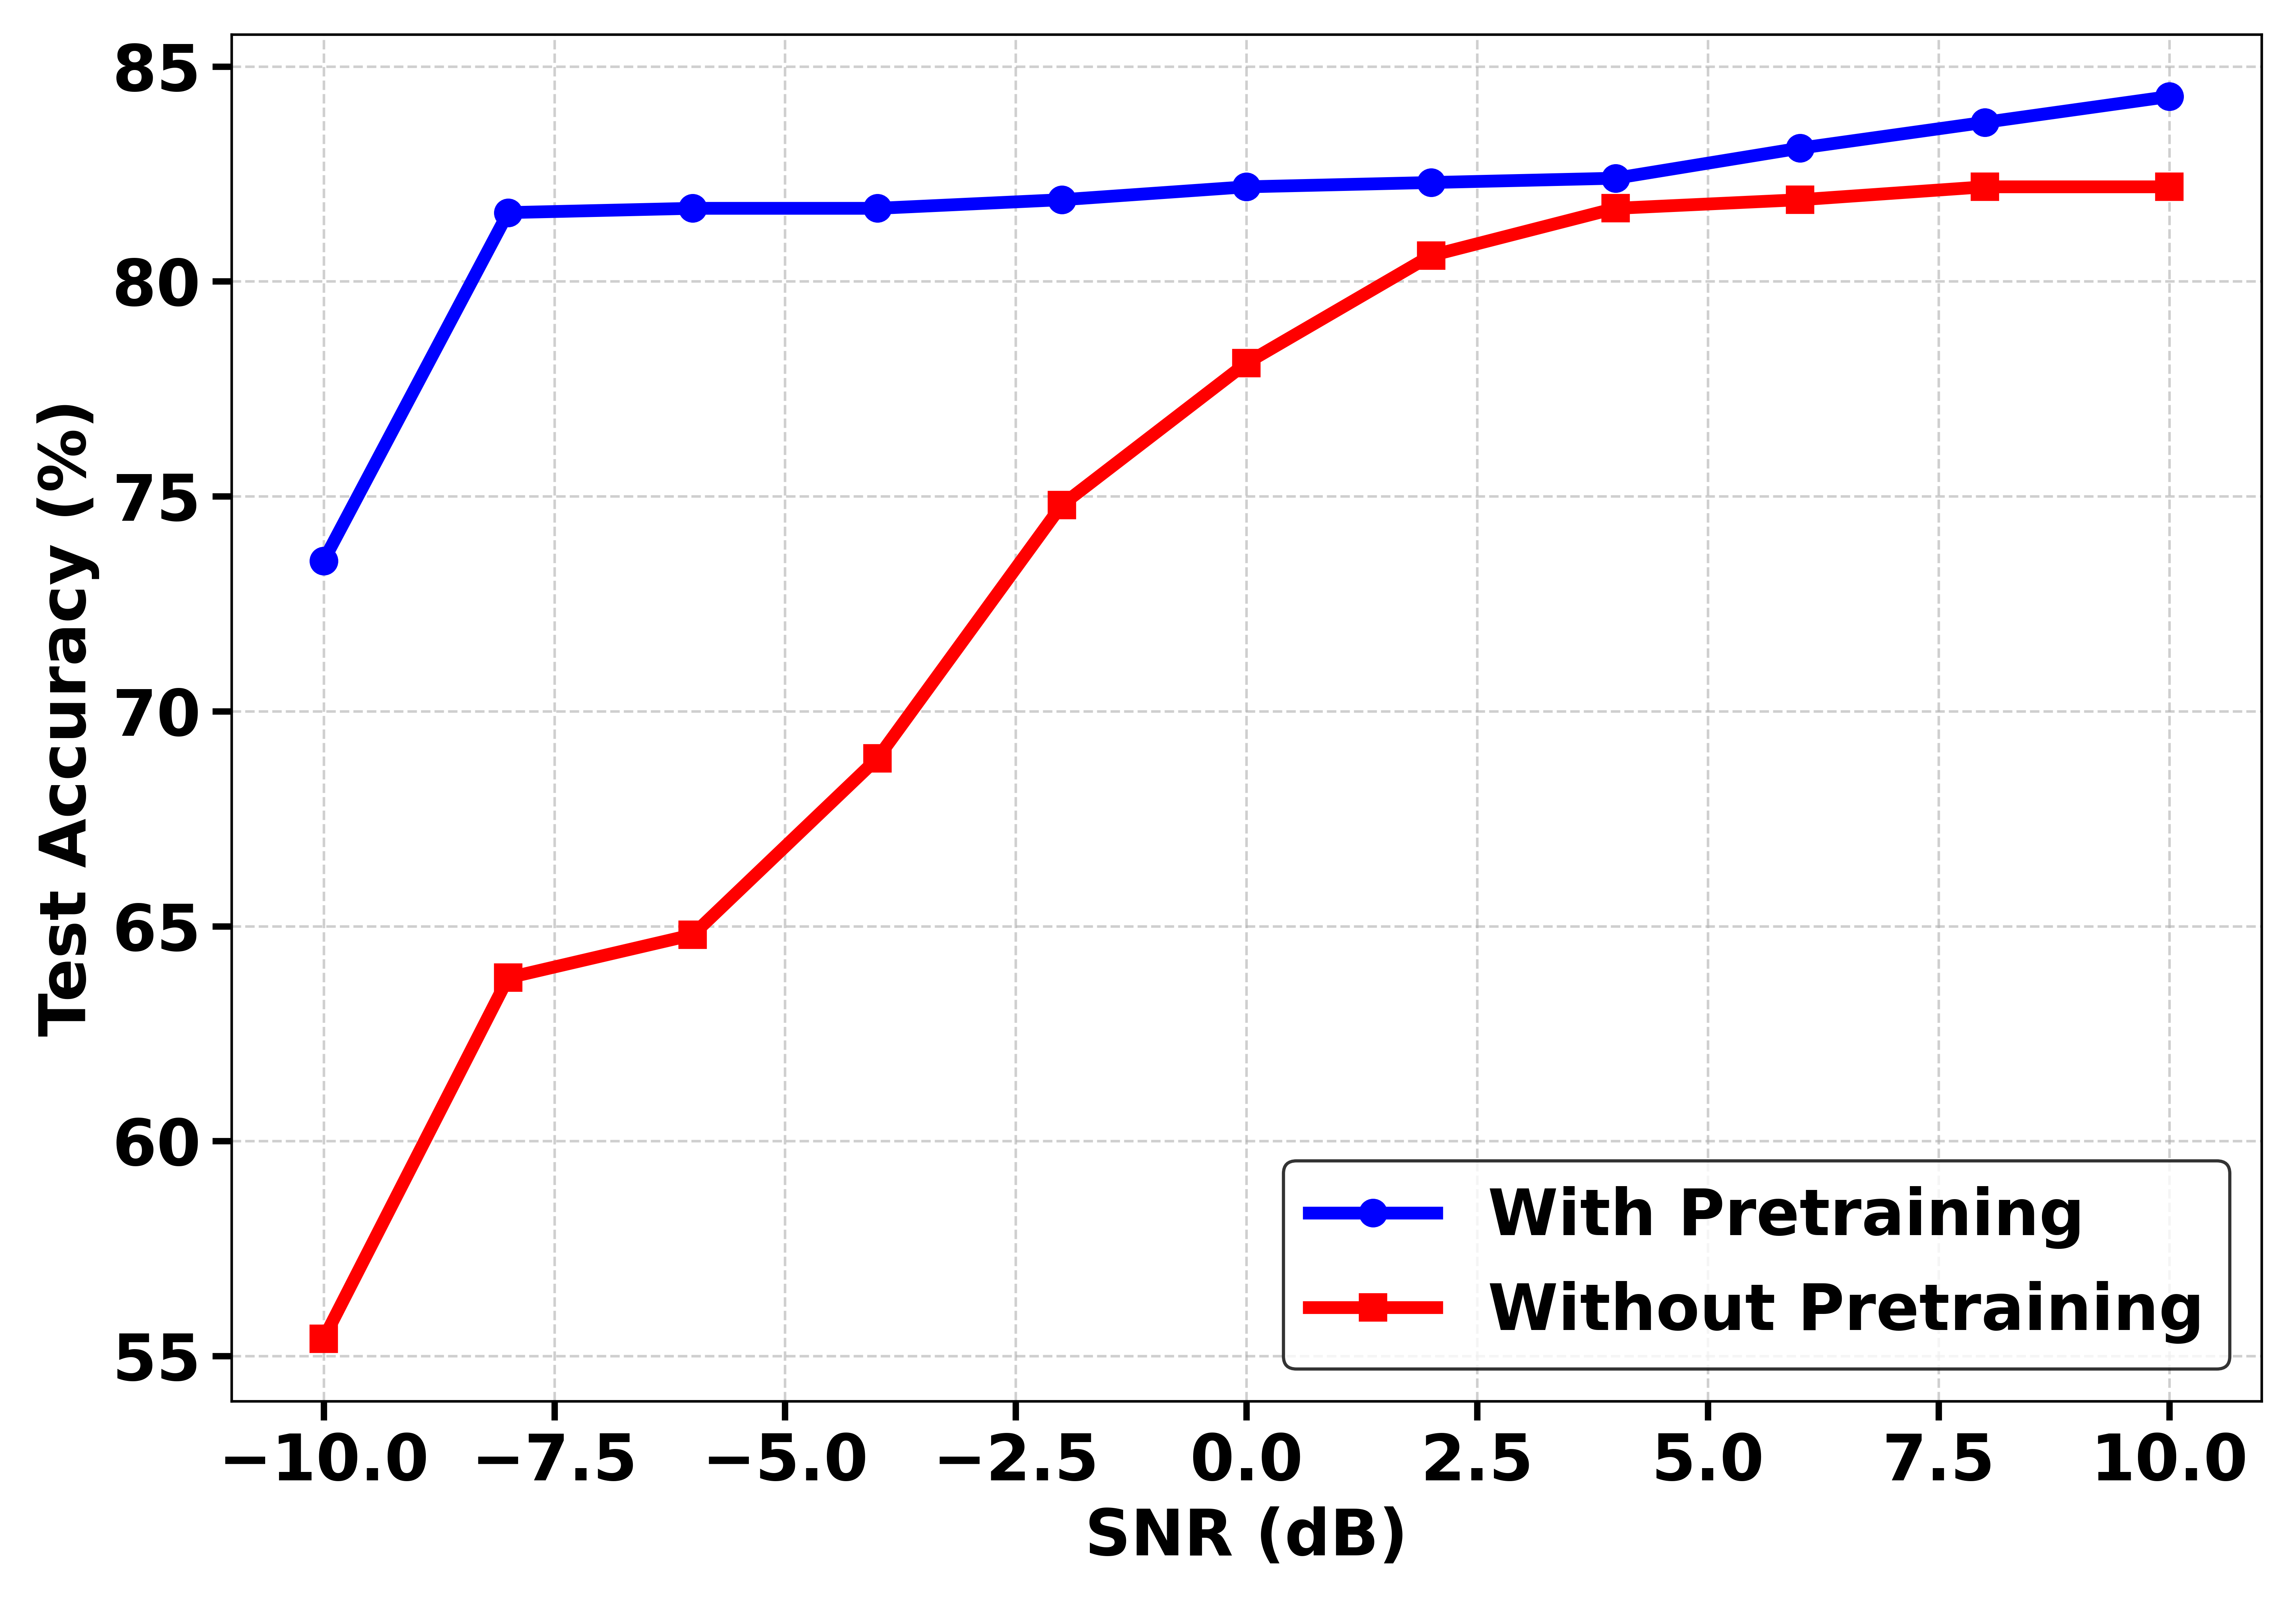
\includegraphics[width=0.85\linewidth]{FIGURES/denomae/plot.png} % Adjust width as needed
    \caption{Classification accuracy for constellation diagrams at different SNRs.}
    \label{accuracy} % Label for referencing
\end{figure}

\subsubsection{Effect of Masking Ratio}

We investigated the impact of masking ratio during pretraining on downstream classification. As shown in Figure \ref{masking}, masking ratio significantly influences performance, with accuracy rising from 79.6\% at 10\% masking to peak at 83.5\% with 75\% masking, before declining to 81.4\% at 80\% and 79.0\% at 90\% masking. This pattern indicates moderate to high masking ratios (60-75\%) compel the model to learn more robust features by reconstructing substantial missing information. Extremely high ratios (\textgreater{80\%}) provide insufficient context for effective reconstruction, while low ratios (\textless{40\%}) fail to sufficiently challenge the model. The optimal approach thus involves masking a significant but not overwhelming portion of input data.

\begin{figure}[htbp]
    \centering
    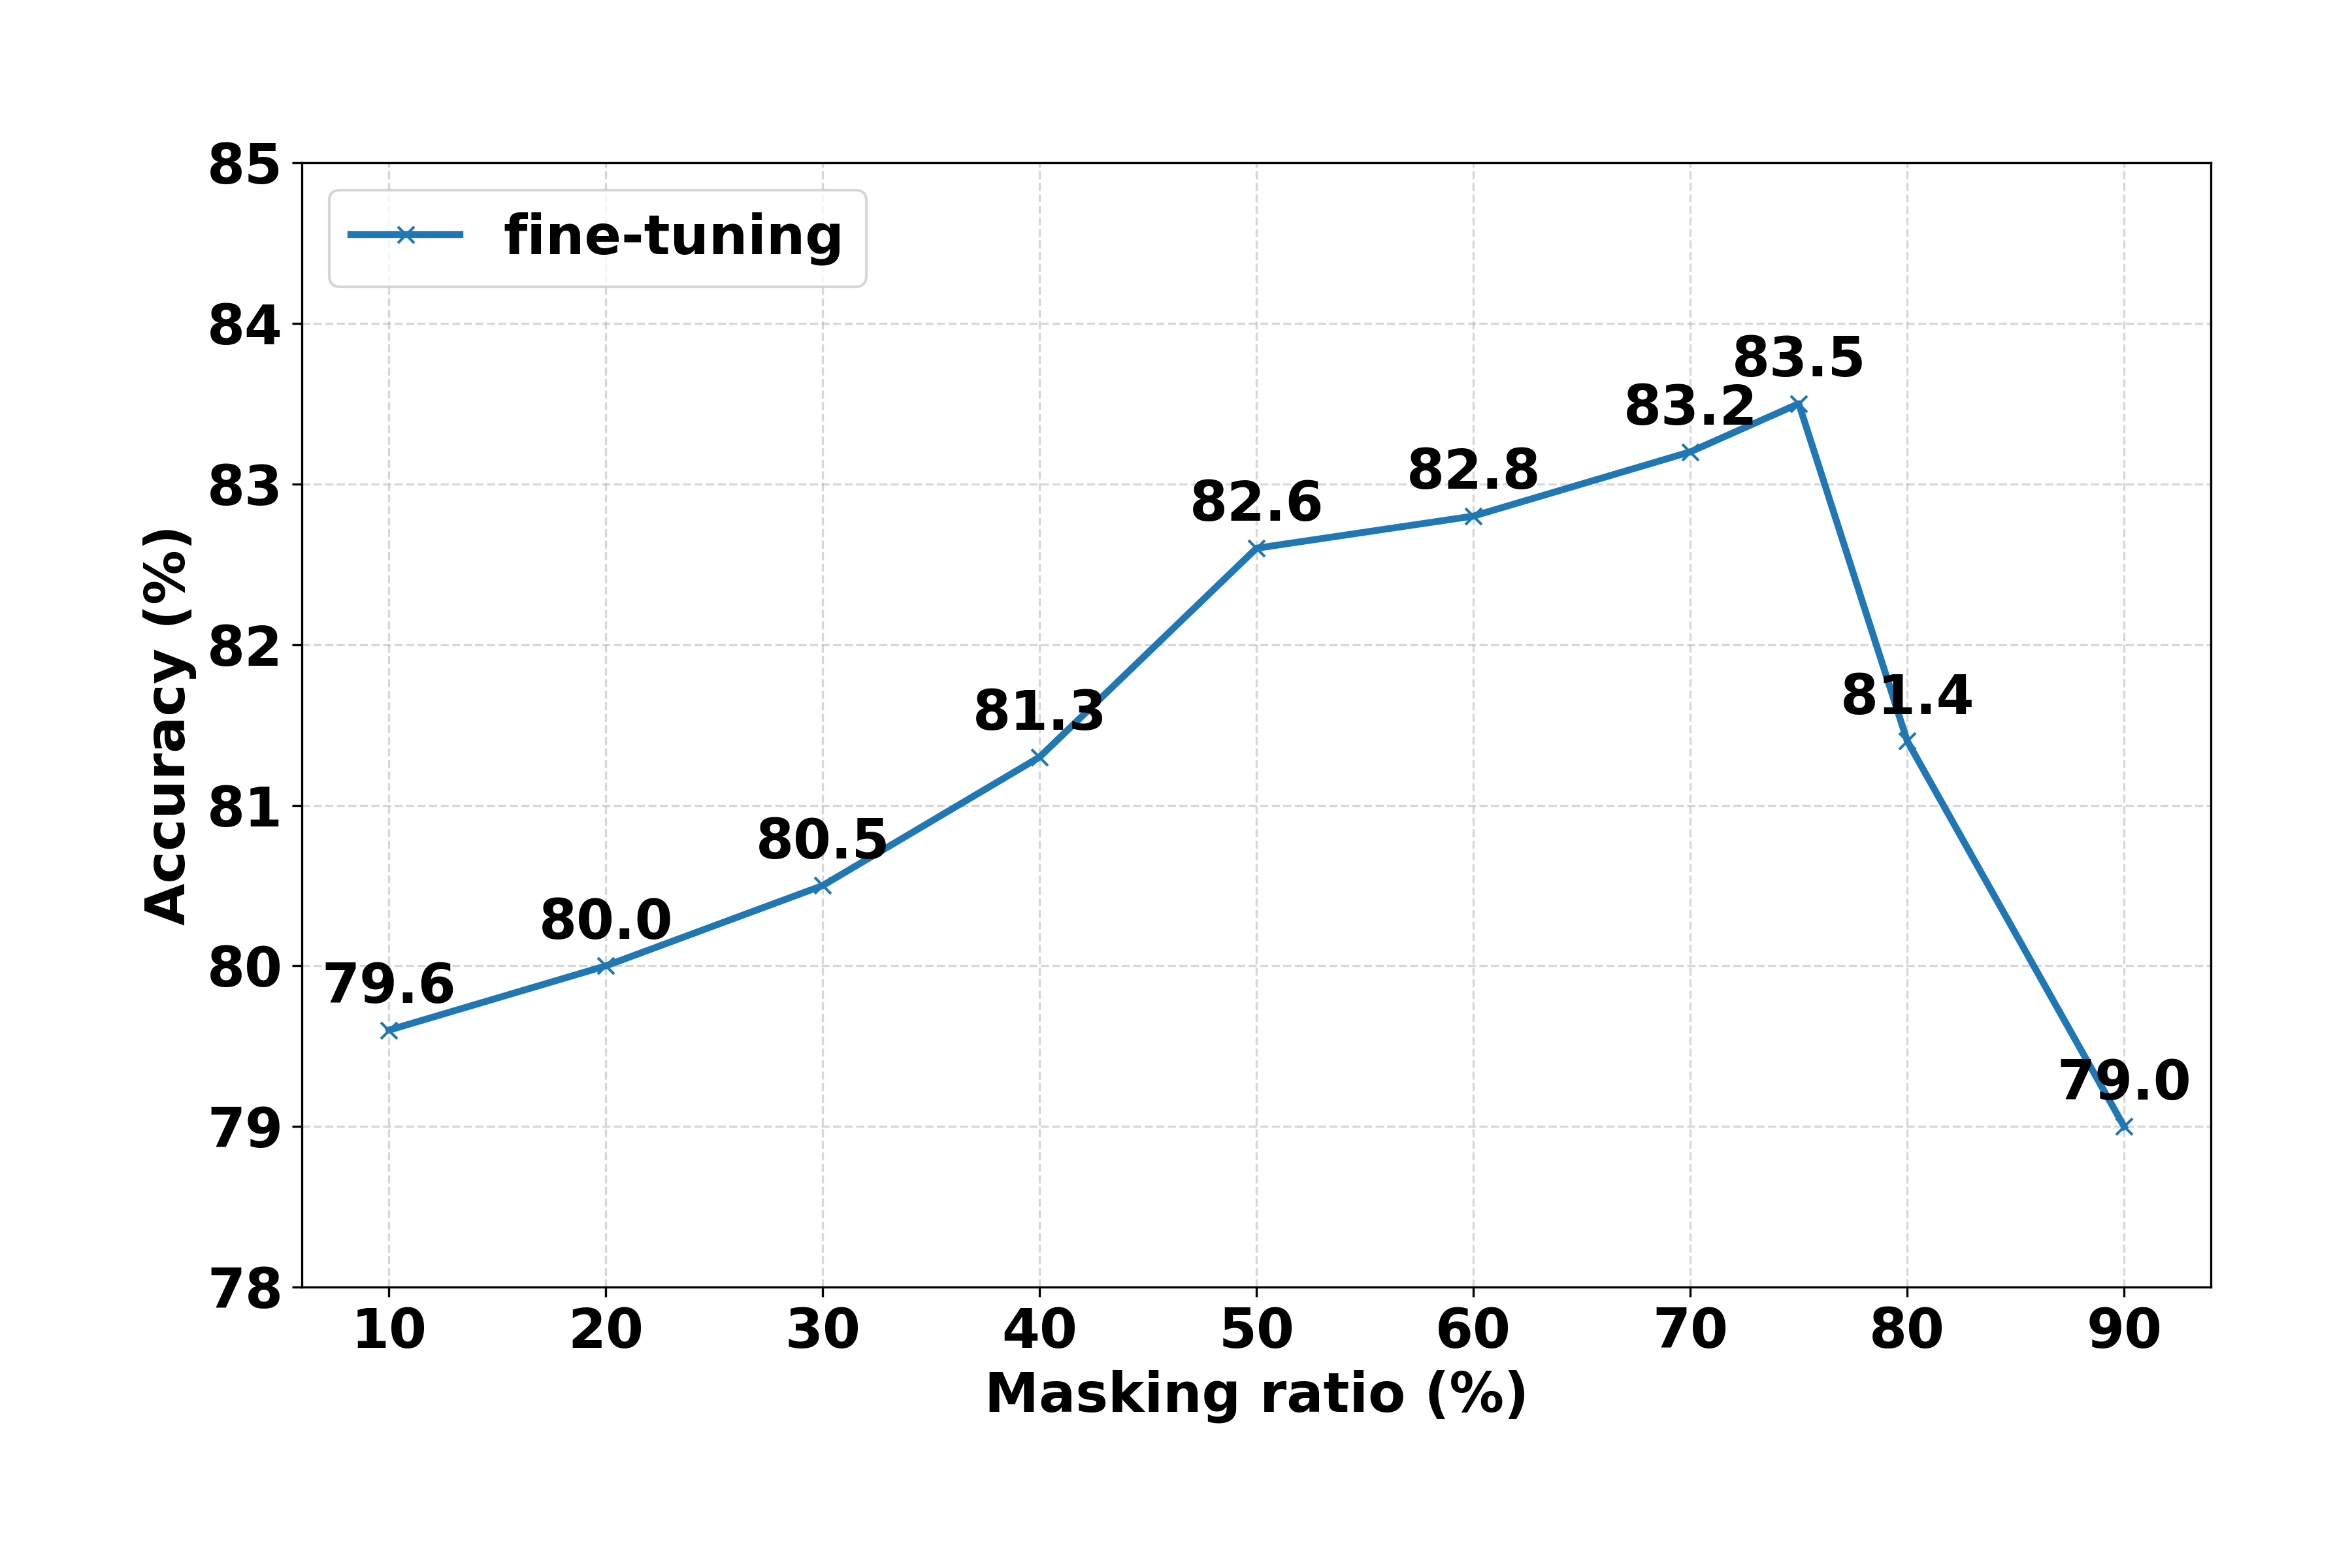
\includegraphics[width=0.9\linewidth]{FIGURES/denomae/mask.png} % Adjust width as needed
    \caption{Effect of masking ratio on fine-tuning accuracy.}
    \label{masking} % Label for referencing
\end{figure}

\subsubsection{Extrapolation on Out-of-bound SNRs}

DenoMAE demonstrates impressive extrapolation capabilities when evaluated on SNR conditions significantly outside its training range. Although trained only on SNR levels above $-10$ dB, the model continues to deliver meaningful reconstruction performance at challenging SNR levels between $-11$ dB and $-20$ dB. As shown in Figure \ref{fig:extrap}, DenoMAE effectively denoises highly noisy input constellation diagrams, making the first two samples visually recognizable. The final sample, while impacted by extreme noise, still approximates the outer shape of the ground truth.

\begin{figure}[htbp]
    \centering
    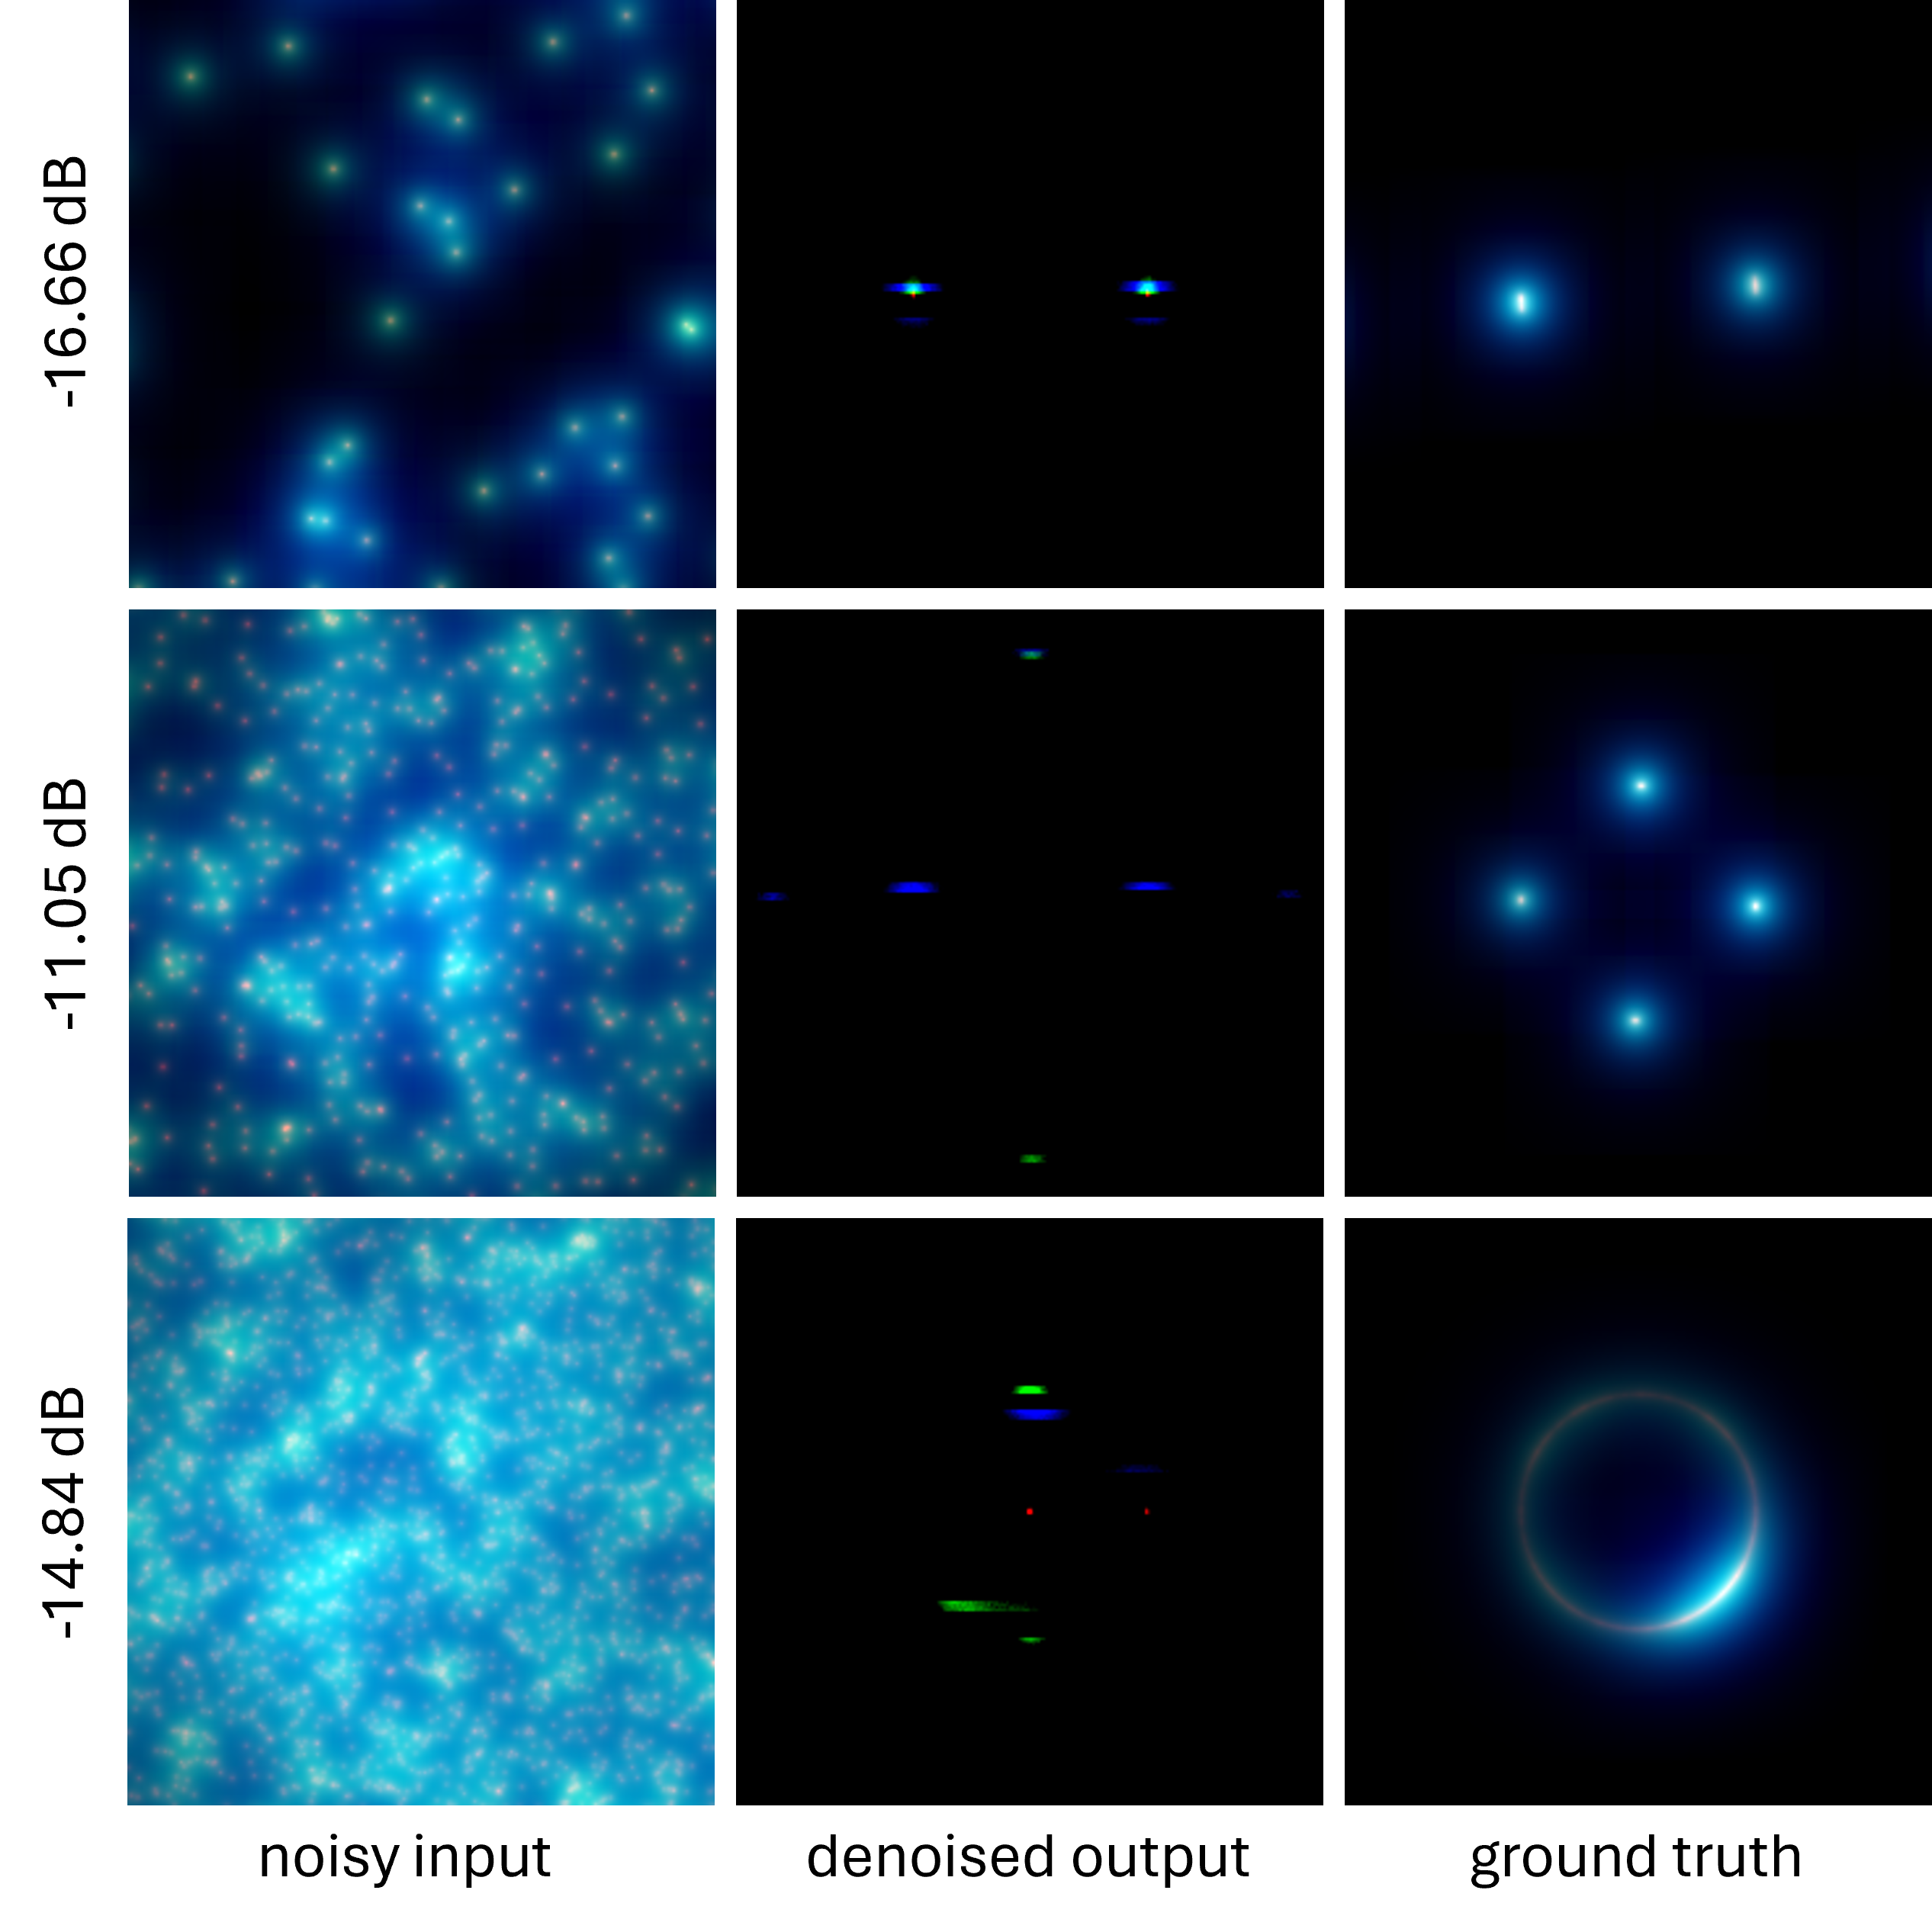
\includegraphics[width=0.8\linewidth]{FIGURES/denomae/extrapolate.png} % Adjust width as needed
    \caption{Extrapolation-ability of DenoMAE on out-of-bound lower SNRs.}
    \label{fig:extrap} % Label for referencing
\end{figure}

\subsubsection{Ablation Study on Modality Impact}

Our shared encoded space enables complementary information from different modalities to enhance each other through cross-modal knowledge transfer. When one modality (e.g., constellation diagrams) is severely corrupted by noise, the model can leverage information from the other modalities (e.g., signals) through this integrated representation. By aligning different views of the same signal in a common space, the model learns to distinguish between noise artifacts and true signal characteristics, significantly improving denoising performance.

Our ablation study on modality impact, detailed in Table \ref{modulations}, reveals the effectiveness of the multimodal approach. The full model with five modalities (noisy image, noisy signal, noiseless image, noiseless signal, and noise) achieves 83.50\% accuracy. Performance degrades gracefully as modalities are removed, with even the single-modality version maintaining 81.30\% accuracy. This suggests that while additional modalities contribute to performance gains, the model maintains robust performance even with reduced modality input, indicating efficient cross-modal learning capabilities.

\begin{table}
    \centering
    \caption{Performance Comparison Across Different Modalities}
    \label{modulations}
    \begin{tabular}{c|c|c|c|c|c}
    \hline
    \multicolumn{2}{c|}{Constellation} & \multicolumn{2}{c|}{Signal} & Noise & Test Accuracy (\%) \\
    \cline{1-4}
    Clean & Noisy & Clean & Noisy &  &  \\
    \hline
    \cline{1-4} 
    \checkmark &  &  &  &  & 81.30 \\
    \checkmark & \checkmark &  &  &  & 81.90 \\
    \checkmark & \checkmark & \checkmark &  &  & 83.20 \\
    \checkmark & \checkmark & \checkmark & \checkmark & & 83.30 \\
    \checkmark & \checkmark & \checkmark & \checkmark & \checkmark & 83.50 \\
    \hline
\end{tabular}
\end{table}
    
\subsubsection{Comparative Analysis}

Table \ref{compare} presents a comparison between DenoMAE and existing modulation classification approaches. Our model achieves 83.5\% accuracy at 0.5 dB SNR, outperforming AlexNet (82.8\% at 2 dB), NMformer (71.6\% at 0.5-4.5 dB), CNN-AMC (50.40\% at -6 dB), and DL-GRF (59\% at 0 dB). DenoMAE demonstrates remarkable data efficiency, requiring only 10,000 pretraining and 1,000 fine-tuning samples—an $80\times$ reduction compared to AlexNet's 800,000 samples and a $10.7\times$ reduction versus NMformer. Notably, DenoMAE maintains 77.50\% accuracy even at -10 dB SNR, highlighting its robust performance in challenging noise conditions.

From a computational perspective, DenoMAE has comparable model complexity to NMformer (both 85.8M parameters) with identical inference time (14.5 ms), yet delivers 11.9\% higher accuracy. While CNN-AMC offers faster inference (0.13 ms) with fewer parameters (1.6M), it achieves lower accuracy and classifies only 4 modulation types versus DenoMAE's 10 classes. Similarly, DL-GRF (23.5M parameters, 10 ms inference) handles only 4 classes. These results demonstrate DenoMAE's exceptional balance between performance, data efficiency, and complexity for real-world wireless communications.

\begin{table}[htbp]
    \centering
    \caption{Comparison of DenoMAE with other modulation classification methods}
    \label{compare}
    \resizebox{\textwidth}{!}{%
    \begin{tabular}{cccccccc}
    \toprule
    \multirow{2}{*}{\textbf{Methods}} &
    \multicolumn{2}{c}{\textbf{Number of samples}} &
    \multirow{2}{*}{\textbf{SNR dB}} &
    \multirow{2}{*}{\textbf{Number of classes}} &
    \multirow{2}{*}{\textbf{Finetuning parameters}} &
    \multirow{2}{*}{\textbf{Inference time (ms)}} &
    \multirow{2}{*}{\textbf{Test accuracy (\%)}} \\
    \cmidrule(lr){2-3}
    & \textbf{Pretraining} & \textbf{Fine-tuning} & & & & & \\ \midrule

    AlexNet\cite{peng2018modulation}  & 800,000 (train) & 8,000 (test)  & 2 & 8 & 22.5M & 2.0 & 82.8 \\
    NMformer \cite{faysal2024nmformer} & 106,800 & 3,000 & 0.5 - 4.5 & 10 & 85.8M & 14.5 & 71.6 \\
    CNN-AMC \cite{meng2018automatic} & 79,200 & 228,060 & -6 & 4 & 1.6M & 0.13 & 50.40 \\
    DL-GRF \cite{sun2022automatic} & 2,000 (train) & 200 (test) & 0 & 4 & 23.5M & 10 & 59 \\
    DenoMAE (\textbf{Ours}) & 10,000 & 1,000 & 0.5 & 10 & 85.8M & 14.5 & 83.5 \\
    DenoMAE (\textbf{Ours}) & 10,000 & 1,000 & -10 & 10 & 85.8M & 14.5 & 77.50 \\

    \bottomrule
    \end{tabular}%
    }
\end{table}

\subsection{Conclusion}

We presented DenoMAE, a multimodal autoencoder framework that achieves state-of-the-art performance in modulation signal denoising while requiring significantly less training data than existing approaches. Our experiments demonstrate that by incorporating multiple modalities and treating noise as an explicit modality, DenoMAE delivers superior classification accuracy and robust performance across varying SNR conditions, including extrapolation to out-of-bound low SNRs. Future work could explore its extension to diverse signal types and optimization for computational efficiency.

% TODO: Omitting DenoMAE2.0 for now.
% \section{Task 3: DenoMAE2.0: Improving Denoising Masked Autoencoders by Classifying Local Patches for Automatic Modulation Classification}

% \subsection{Introduction}

% Semi-supervised models have emerged as a transformative paradigm in machine learning, addressing the high costs associated with data labeling \cite{zhang2024maskmatch, pmlr-v182-poulain22a}. A prevalent approach in semi-supervised learning involves pretraining models on large amounts of unlabeled data, which are abundant and readily available \cite{chen2020bigselfsupervisedmodelsstrong, xu2022revisitingpretrainingsemisupervisedlearning}. These models leverage unlabeled data to capture underlying patterns and structures, enabling effective representation learning. Consequently, the pretrained models exhibit improved performance and faster adaptation during downstream tasks, making semi-supervised learning a cost-efficient and scalable solution for real-world applications \cite{cai2022semisupervisedvisiontransformersscale}.

% Recent advancements in self-supervised learning have achieved remarkable success through representation learning~\cite{grill2020bootstrap, chen2020exploring}, contrastive learning~\cite{chen2020simple, khosla2020supervised}, and masking strategies \cite{yin2024stablemask}. Among these, masking strategies leveraging Vision Transformer (ViT) \cite{dosovitskiy2020image} architectures have set new benchmarks in tasks such as classification , reconstruction, and image analysis. Masked Autoencoders (MAE) \cite{he2022masked}, in particular, have demonstrated significant potential by randomly masking portions of input data and training models to reconstruct the missing information. Despite their success, traditional MAE methods predominantly emphasize global reconstruction objectives, often neglecting fine-grained local patterns that are critical for enhancing representation learning \cite{yue2023understanding}.

% Masking strategies are particularly beneficial for pretraining in wireless communication for Autometic Modulation Classification (AMC), where acquiring labeled data is challenging due to privacy and copyright constraints \cite{zhao2024vit, zayat2023transformer}. Moreover, communication signals are often corrupted by environmental noise and channel losses, making robust representation learning essential. DenoMAE \cite{faysal2025denomae} addresses these challenges by integrating masking and denoising within a unified framework, leveraging masked modeling to enhance performance. While DenoMAE has demonstrated exceptional results in denoising and achieving strong classification accuracy, it inherits the fundamental principles of MAE, which focus primarily on global representation learning through masking. Consequently, the model remains unaware of the specific locations of the masked inputs, limiting its ability to fully exploit fine-grained local patterns and unlock the complete potential of representation learning.

% We present DenoMAE2.0, an enhanced framework that introduces a novel local patch classification objective alongside the traditional reconstruction task. Our approach differs from existing methods by treating visible patches as distinct classes based on their spatial positions, enabling the model to learn position-aware local features while maintaining global coherence. This dual-objective strategy encourages the model to capture both structural and semantic information, leading to more robust and informative representations.

% \subsection{Contributions}

% The key contributions of our work are threefold:

% \begin{itemize}
%     \item We propose a novel architecture that combines denoising reconstruction with local patch classification, enabling simultaneous learning of global and local features.
%     \item We introduce a position-based classification strategy that leverages spatial information to enhance representation learning without requiring additional labels.
%     \item Through extensive experiments, we demonstrate that DenoMAE2.0 achieves superior performance on various downstream and transfer learning tasks compared to traditional MAE and DenoMAE approaches, particularly in scenarios with limited labeled data.
% \end{itemize}

% Our results indicate that the integration of local patch classification significantly improves the quality of learned representations, leading to better denoising, generalization and faster convergence during fine-tuning. The proposed method not only advances the state-of-the-art in self-supervised learning but also provides insights into the importance of incorporating local structural information in representation learning frameworks.

% \subsection{Related Work}

% This section discusses recent advancements in modulation classification and self-supervised learning methods, with a focus on their applications in wireless communication systems. We examine how these approaches have evolved from traditional feature engineering to modern deep learning architectures, highlighting the growing importance of self-supervised techniques in addressing data scarcity challenges.

% \subsubsection{AMC in Wireless Communication}

% Early AMC methods primarily relied on expert-crafted features extracted from constellation diagrams and signal statistics, utilizing likelihood-based approaches and higher-order statistics to classify modulation schemes \cite{dobre2007survey}. Constellation diagrams, which visually represent symbol distributions in the complex plane, have been a fundamental tool for feature extraction in classical AMC. These diagrams illustrate the effects of noise, interference, and channel distortions, making them valuable for differentiating modulation schemes based on clustering patterns, symbol dispersion, and trajectory structures \cite{o2018over}. 

% The advent of deep learning revolutionized AMC by enabling models such as CNNs to operate directly on I/Q samples and constellation diagrams, bypassing the need for manual feature engineering \cite{zhang2021efficient}. Deep learning approaches leverage spatial patterns in constellation diagrams, learning robust representations that improve classification accuracy over conventional methods \cite{doan2020learning}. More recent advancements incorporate attention mechanisms and transformer architectures to capture long-range dependencies in signal patterns \cite{hamidi2021mcformer}. However, these deep learning-based AMC methods often require large labeled datasets and exhibit limited generalization across varying channel conditions, posing challenges for real-world deployment \cite{ya2022large}.

% \subsubsection{Self-Supervised Learning Approaches}

% The evolution of modern Self-Supervised Learning (SSL) strategies in deep learning and wireless communication has progressed through distinct phases, starting with contrastive learning, followed by representation learning, and more recently, the adoption of masking techniques.  Contrastive learning exemplified by SimCLR~\cite{chen2020simple} and MoCo \cite{he2020momentumcontrastunsupervisedvisual}, relied on distinguishing positive and negative sample pairs to learn robust feature representations, proving effective in image and signal processing tasks. This was followed by representation learning methods \cite{grill2020bootstrap, berthelot2019mixmatch}, which eliminated the need for negative samples by aligning representations of augmented views, enhancing efficiency and scalability. More recently, masking-based techniques \cite{devlin2019bert, he2022masked} have gained prominence by reconstructing masked portions of inputs, offering a powerful framework for learning from incomplete data \cite{faysal2025denomae}.

% In wireless communication, semi-supervised learning are particularly useful for modulation classification, where labeled data is often scarce due to the complexity of signal environments. Ma et al. \cite{ma2024refined} developed a semi-supervised framework leveraging pseudo-labeling, where a model trained on limited labeled modulation samples generates labels for unlabeled data, iteratively refining its performance across diverse modulation schemes. Another approach by Sifaou and Simeone \cite{sifaou2024semisupervisedlearningcrosspredictionpoweredinference} exploits Cross-Prediction-Powered Inference (CPPI) to enhance semi-supervised learning by mitigating the bias of synthetic labels. Their method refines ML-based predictions through tuned CPPI and meta-CPPI, achieving improved performance in tasks like beam alignment and indoor localization, particularly when labeled data is scarce. More related SSL methods in wireless communication includes convolution \cite{zhang2024sswsrnetsemisupervisedfewshotlearning, ermis2022cnn, pmlr-v77-longi17a} and transformer \cite{kong2023transformer, ren2022sigtefficientendtoendmimoofdm, kunde2023transformers} based SSLs.

% \subsection{Methodology: DenoMAE2.0}

% The overall framework of the proposed DenoMAE2.0 is illustrated in Figure \ref{fig:denomae2}. DenoMAE2.0 consists of three components: encoder, reconstruction denoising decoder, and local patch classification head. There are two complementary objectives: the denoising reconstruction objective and the local patch classification classification objective. Details are provided in Algorithm~\ref{lst:DenoMAE2.0} and introduced as follows.

% \begin{figure*}[ht]
%     \centering
%     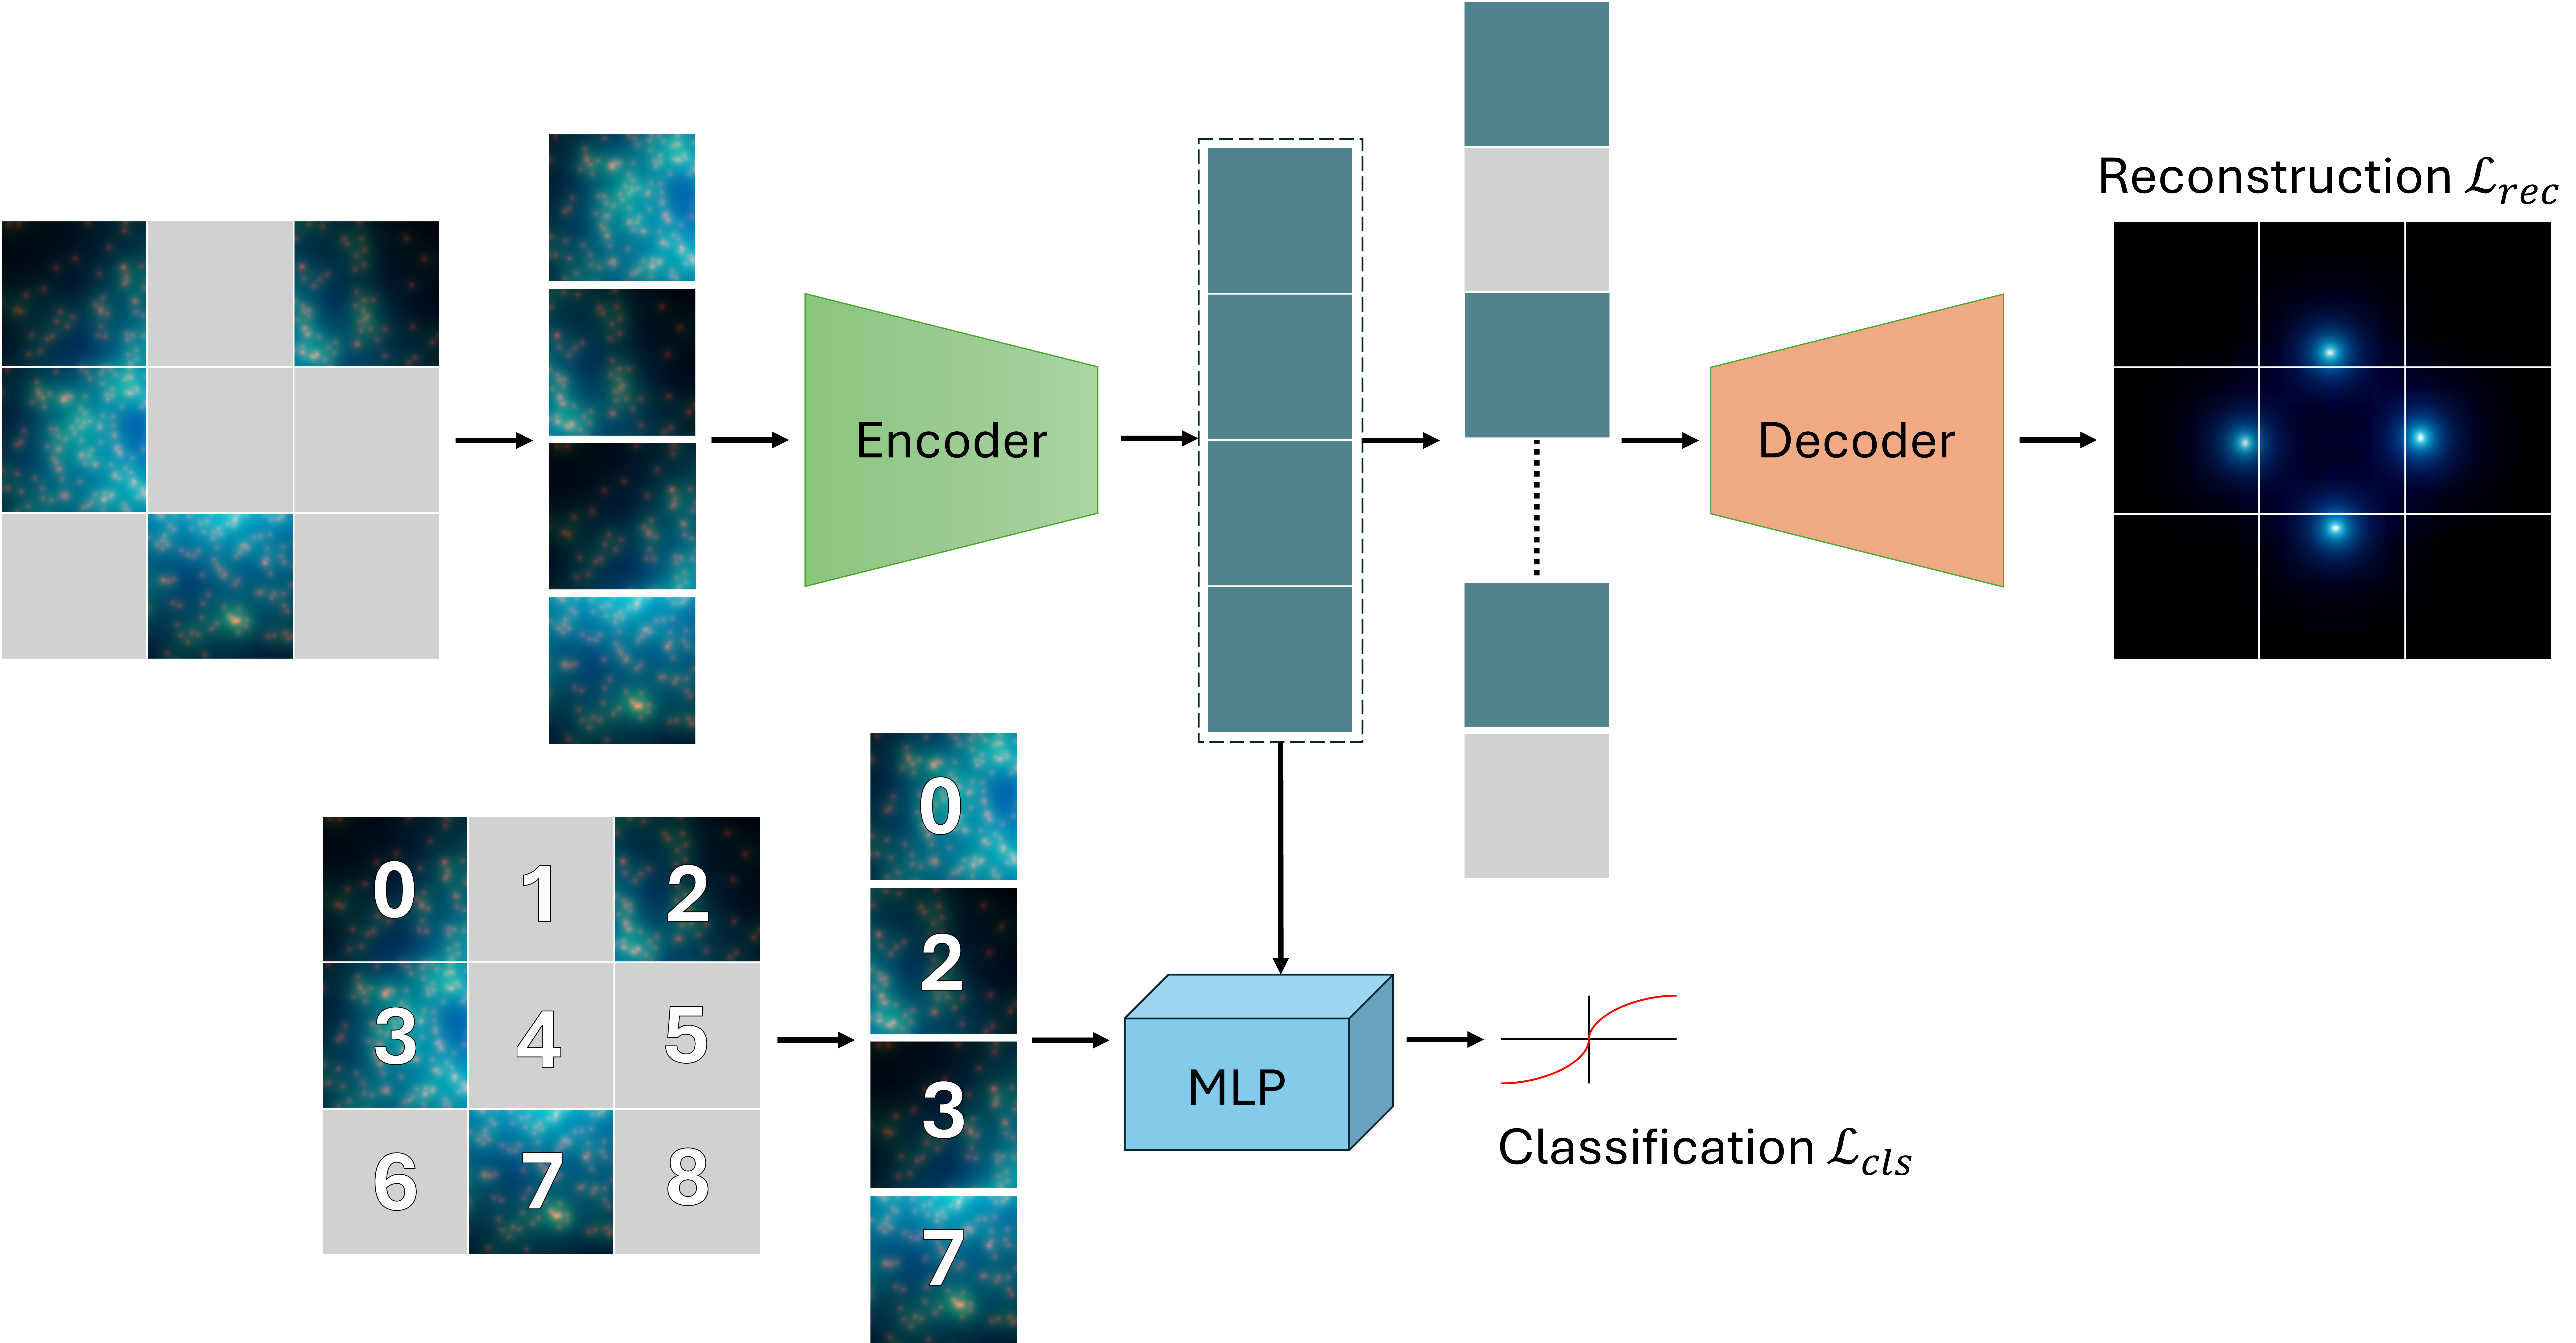
\includegraphics[width=0.9\textwidth]{FIGURES/denomae2/flow_con.png}
%     \caption{DenoMAE2.0 architecture overview: The model consists of an encoder-decoder architecture. The encoder processes visible patches and mask tokens, producing patch-level features for reconstruction and classification. The decoder generates reconstructed patches, while the classification head predicts patch position based on visible patch features.}
%     \label{fig:denomae2}
% \end{figure*}

% \subsubsection{Masking Strategy and Encoder Architecture}


% Consider an input image \(\mathbf{x} \in \mathbb{R}^{H \times W \times C}\). We first partition \(\mathbf{x}\) into 
% \begin{equation}
% N \;=\; \frac{H\,W}{P^2}
% \label{eq:num_patches}
% \end{equation}
% non-overlapping patches, each of size \(P \times P\). Let \(\mathbf{x}_p \in \mathbb{R}^{N \times (P^2\,C)}\) be the flattened patches. A linear projection \(E_{\mathrm{patch}}\) then maps these patches into a \(d\)-dimensional embedding space:
% \begin{equation}
% \mathbf{z}_p \;=\; E_{\mathrm{patch}}\bigl(\mathbf{x}_p\bigr) 
% \;\in\; 
% \mathbb{R}^{N \times d}.
% \label{eq:patch_embed}
% \end{equation}
% To preserve spatial order, we add learnable positional embeddings \(\mathbf{p} \in \mathbb{R}^{N \times d}\), forming the initial token sequence
% \begin{equation}
% \mathbf{Z}^{(0)} 
% \;=\; 
% \mathbf{z}_p 
% \;+\; 
% \mathbf{p}.
% \label{eq:pos_embed}
% \end{equation}

% A random masking operator \(\mathcal{M}_{r}\) discards a fraction \(r\) of these tokens to yield the visible tokens \(\mathbf{Z}_{v}\). The masked tokens \(\mathbf{Z}_{m}\) are replaced by mask tokens in the decoder but are omitted here in the encoder. Let \(\mathcal{E}\) denote the ViT-based encoder with \(L\) Transformer layers. Each layer \(\ell\) applies multi-head self-attention (MSA) and a feed-forward network (FFN) to the visible tokens:
% \begin{align}
% \mathbf{Z}_{v}^{(\ell)} 
% &=\; 
% \mathbf{Z}_{v}^{(\ell-1)} 
% \;+\;
% \mathrm{MSA}
% \!\Bigl(\mathrm{LN}\bigl(\mathbf{Z}_{v}^{(\ell-1)}\bigr)\Bigr),
% \label{eq:msa}
% \\[6pt]
% \mathbf{Z}_{v}^{(\ell)} 
% &=\; 
% \mathbf{Z}_{v}^{(\ell)} 
% \;+\;
% \mathrm{FFN}
% \!\Bigl(\mathrm{LN}\bigl(\mathbf{Z}_{v}^{(\ell)}\bigr)\Bigr).
% \label{eq:ffn}
% \end{align}
% After \(L\) layers, the encoder produces latent representations
% \begin{equation}
% \mathbf{q}_{v} 
% \;=\; 
% \mathcal{E}\bigl(\mathbf{Z}_{v}\bigr),
% \label{eq:encoder_output}
% \end{equation}
% which are subsequently used for both reconstruction in the decoder and the auxiliary classification of unmasked patches.


% \subsubsection{Decoder Architecture and Reconstruction}

% To reconcile the difference between the visible token set 
% \(\mathbf{Z}_{v}\) (equation \eqref{eq:encoder_output}) and the full 
% patch set of size \(N\) (equation \eqref{eq:num_patches}), we introduce 
% learnable \emph{mask tokens} at the masked positions. These tokens, 
% which share a single learned embedding, act as placeholders for the 
% missing patches. Formally, let 
% \(\mathbf{M} \in \mathbb{R}^{|\mathcal{I}_m| \times d}\) be the mask token 
% embeddings corresponding to the set of masked indices \(\mathcal{I}_m\), 
% where \(\mathcal{I}_v \cup \mathcal{I}_m = \{1,2,\dots,N\}\) and 
% \(\mathcal{I}_v \cap \mathcal{I}_m = \varnothing\). We concatenate the 
% visible patch embeddings \(\mathbf{q}_{v}\) and \(\mathbf{M}\), then add 
% positional embeddings to form the decoder input:
% \begin{equation}
%     \mathbf{Z}_{d}^{(0)}
%     \;=\;
%     \mathrm{Shuffle}\!\Bigl(\bigl[\mathbf{q}_{v} \;\Vert\; \mathbf{M}\bigr]\Bigr)
%     \;+\; 
%     \mathbf{p}_{d},
% \label{eq:decoder_input}
% \end{equation}
% where \(\mathbf{p}_{d} \in \mathbb{R}^{N \times d}\) denotes the positional 
% embeddings for the decoder, and \(\mathrm{Shuffle}(\cdot)\) reorders the tokens 
% to match their original patch indices.

% The decoder consists of a Transformer stack with fewer layers and heads 
% than the encoder for computational efficiency. Denote the decoder by 
% \(\mathcal{D}\). Each layer follows the same multi-head self-attention and 
% feed-forward structure described in \eqref{eq:msa}--\eqref{eq:ffn}, yielding 
% a final decoder output \(\mathbf{Z}_{d}^{(L')}\). A linear projection 
% \(\mathbf{W}_{\mathrm{out}} \in \mathbb{R}^{d \times (P^2\,C)}\) maps each token 
% to the original patch dimension, thereby producing reconstructed patches:
% \begin{equation}
%     \widehat{\mathbf{x}}
%     \;=\;
%     \bigl[\mathbf{Z}_{d}^{(L')} \mathbf{W}_{\mathrm{out}}\bigr]
%     \;\in\;
%     \mathbb{R}^{N \times (P^2\,C)}.
% \label{eq:decoder_out}
% \end{equation}

% We adopt a \emph{masked} mean squared error (MSE) loss to focus the 
% reconstruction objective solely on the masked patches. Let 
% \(\widehat{\mathbf{x}}_{m}\) and \(\mathbf{x}_{m}\) respectively denote the 
% reconstructed and ground-truth patches for the set of masked indices 
% \(\mathcal{I}_m\). The reconstruction loss is
% \begin{equation}
%     \mathcal{L}_{\mathrm{rec}}
%     \;=\;
%     \frac{1}{|\mathcal{I}_m|}
%     \sum_{i \in \mathcal{I}_m}
%     \bigl\|\widehat{\mathbf{x}}_{m}^{(i)} - \mathbf{x}_{m}^{(i)}\bigr\|^{2},
% \label{eq:rec_loss}
% \end{equation}
% where \(\|\cdot\|\) denotes the Euclidean norm. By confining 
% \(\mathcal{L}_{\mathrm{rec}}\) to the masked regions, the decoder is compelled 
% to infer the missing patches from context, thus enhancing its denoising 
% capabilities.


% \subsubsection{Patch Classification Head}

% While the decoder focuses on reconstructing masked patches,
% the visible patch embeddings \(\mathbf{q}_{v}\) 
% (equation~\eqref{eq:encoder_output})
% can also facilitate a classification objective. Unlike 
% traditional classification tasks where a single label is assigned 
% per image, we treat \emph{each unmasked patch} as a distinct class. 
% Let \(\mathbf{q}_{v} \in \mathbb{R}^{|\mathcal{I}_v| \times d}\) 
% represent the visible token embeddings corresponding to the set of 
% indices \(\mathcal{I}_v\). We define the total number of classes by
% \begin{equation}
%   N_{\mathrm{cls}}
%   \;=\;
%   N \cdot \bigl(1 - r\bigr),
% \label{eq:num_classes}
% \end{equation}
% where \(N\) is the total number of patches 
% (equation~\eqref{eq:num_patches}), and \(r\) is the masking ratio. 
% Hence, each visible patch is assigned a unique position-based label.

% To learn these labels, we project the visible embeddings 
% \(\mathbf{q}_{v}\) via a simple linear layer 
% \(\mathbf{W}_{\mathrm{cls}} \in \mathbb{R}^{d \times N_{\mathrm{cls}}}\), 
% yielding logits \(\mathbf{p} \in \mathbb{R}^{|\mathcal{I}_v| \times 
% N_{\mathrm{cls}}}\). The classification loss \(\mathcal{L}_{\mathrm{cls}}\) 
% is defined via cross-entropy:
% \begin{equation}
%   \mathcal{L}_{\mathrm{cls}}
%   \;=\;
%   \mathrm{CE}\bigl(\mathbf{p}, \mathbf{y}\bigr),
% \label{eq:cls_loss}
% \end{equation}
% where \(\mathbf{y}\) denotes the ground-truth position labels for 
% the visible patches. By jointly optimizing \eqref{eq:rec_loss} 
% and \eqref{eq:cls_loss}, the model learns richer representations 
% of both global context and local patch identities.

% \subsubsection{Overall Objective}

% DenoMAE2.0 optimizes a combination of reconstruction and classification losses, enabling simultaneous learning of fine-grained local and global features. The overall loss function is formulated as a weighted sum:

% \begin{equation}
%     \mathcal{L} = \lambda_{\text{rec}}\mathcal{L}_{\text{rec}} + \lambda_{\text{cls}}\mathcal{L}_{\text{cls}}
% \end{equation}

% where $\lambda_{\text{rec}}$ and $\lambda_{\text{cls}}$ are balancing weights for the reconstruction and classification objectives, respectively. Through empirical validation (see Table~\ref{tab:weights_accuracy}), we set $\lambda_{\text{rec}} = 1.0$ and $\lambda_{\text{cls}} = 0.1$.

% \subsubsection{Fine-Tuning for Classification Tasks}

% After pre-training DenoMAE2.0 on unlabeled data, we fine-tune the
% model for downstream classification. First, we discard the decoder
% and the patch classification head, retaining only the encoder
% (equation \eqref{eq:encoder_output}). During fine-tuning, we provide the
% encoder with full, unmasked images, thereby omitting the masking
% mechanism. Let \(\{ \mathbf{z}_{i} \}_{i=1}^{N}\) denote the patch
% embeddings produced by the encoder for each input, where \(N\)
% remains as defined in \eqref{eq:num_patches}. We apply mean pooling:
% \begin{equation}
%   \label{eq:global_representation}
%   \mathbf{z}
%   \;=\;
%   \frac{1}{N}
%   \sum_{i=1}^{N}
%   \mathbf{z}_{i},
% \end{equation}
% to obtain a global image representation. 

% This \(\mathbf{z}\) is then
% passed through a lightweight multi-layer perceptron (MLP) head, defined as:

% \begin{equation}
% f_{\text{cls}}(\mathbf{z}) = W_3 \cdot \text{GELU}(W_2 \cdot \text{GELU}(W_1 \cdot \mathbf{z}))
% \end{equation}

% where $\mathbf{z} \in \mathbb{R}^{d_{\text{encoder}}}$ is the image representation, $W_1 \in \mathbb{R}^{512 \times d_{\text{encoder}}}$, $W_2 \in \mathbb{R}^{256 \times 512}$, and $W_3 \in \mathbb{R}^{C \times 256}$ with $C$ denoting the number of classes in the dataset. Dropout with rate $p=0.1$ is applied after each GELU activation \cite{hendrycks2016gaussian}.

% This representation is subsequently passed through the classification head to produce final predictions $\mathbf{y} = f_{\text{cls}}(\mathbf{z})$. By default, we maintain frozen encoder parameters during fine-tuning to preserve pre-trained representations, although this constraint can be relaxed for end-to-end optimization when sufficient labeled data is available.

% \begin{algorithm}[htbp]
%     \caption{DenoMAE2.0, PyTorch-like pseudo code}
%     \label{lst:DenoMAE2.0}
%     \begin{algorithmic}[1]
%     \small
%     \Statex \textcolor{green!60!black}{\# f\_enc, f\_dec: encoder, decoder}
%     \Statex \textcolor{green!60!black}{\# f\_mlp: patch classification head}
%     \Statex \textcolor{green!60!black}{\# mask\_r: mask ratio}
%     \Statex \textcolor{green!60!black}{\# lambda\_rec, lambda\_cls: loss function weights}
%     \Statex
    
%     \For{\texttt{x, \_ in loader}}  \Comment{\textcolor{green!60!black}{ load a minibatch}}
%         \State \texttt{x = patch\_emb(x)}  \Comment{\textcolor{green!60!black}{ patch embeddings}}

%         \text{}

%         \State \texttt{x\_v,x\_m,mask\_ids = masking(x,mask\_r)} \Comment{\textcolor{green!60!black}{ random visible and masked patches}}

%         \State \texttt{q\_v = f\_enc(x\_v)}  \Comment{\textcolor{green!60!black}{ unmasked patch features}}
%         \State \texttt{logits = f\_mlp(q\_v)}  \Comment{\textcolor{green!60!black}{ predicted patch labels}}
%         \State \texttt{k\_m = f\_dec(q\_v)}  \Comment{\textcolor{green!60!black}{ pixels reconstruction}}

%         \text{}

%         \State \texttt{labels = class\_labels(mask\_ids)} \Comment{\textcolor{green!60!black}{  class labels generatio}}
%         \State \texttt{loss = lambda\_rec *}
%         \Statex  \texttt{~~~~~~~~~~~~~~~rec\_loss(k\_m, x\_m) +}
%         \Statex \texttt{~~~~~~~~~~~~~~~lambda\_cls * }
%         \Statex \texttt{~~~~~~~~~~~~~~~cls\_loss(logits, labels)}
%         \State \texttt{loss.backward()}
%         \State \texttt{optimizer.update()}  \Comment{\textcolor{green!60!black}{ optimizer update}}
%     \EndFor

%     \text{}

%     \Statex {{\bf function} class\_labels(mask\_ids):}  \Comment{\textcolor{green!60!black}{ label generalization for patches}}
%         \State \texttt{~~~classes = $(($img\_size//patch\_size$)^2$) *}
%         \Statex  \texttt{~~~~~~~~~~~~~(1 - mask\_r)}
%         \State \texttt{~~~labels =} \Comment{\textcolor{green!60!black}{ 0: visible, 1: masked}}
%         \Statex \texttt{~~~~~~~~~classes[mask, where mask == 0]}  
%         \State \texttt{{\bf ~~~~~return} labels}
%     \Statex

    
%     \Statex {{\bf function} rec\_loss(k, x):}  \Comment{\textcolor{green!60!black}{ reconstruction loss}}
%         \State \texttt{~~~x = normalize(x)}  \Comment{\textcolor{green!60!black}{ normalize patches}}
%         \State \texttt{~~~loss = $($k - x$)^2$}  \Comment{\textcolor{green!60!black}{ MSE loss}}
%         \State \texttt{{\bf ~~~~~return} loss}
%     \Statex


%     \Statex {{\bf function} cls\_loss(logits, tgt):}  \Comment{\textcolor{green!60!black}{ classification loss}}
%         \State \texttt{~~~loss = CrossEntropyLoss(logits, tgt)}
%         \State \texttt{{\bf ~~~~~return} loss}

%     \Statex \text{}

% \end{algorithmic}

% \textbf{Note:} `patch\_emb' and `masking' functions are omitted for brevity. For full implementation, see: \url{https://github.com/atik666/denoMAE2}.

% \end{algorithm}

% \subsection{Datasets}

% Our experimental datasets incorporate a core collection of modulation samples evenly distributed across signal-to-noise ratios (SNRs) ranging from -10 dB to 10 dB for pretraining.  These datasets span ten modulation schemes commonly encountered in wireless communication systems, carefully curated to represent realistic operational scenarios while maintaining computational tractability. The balanced distribution across SNR levels enables thorough evaluation of model robustness under varying noise conditions.

% \subsubsection{Constellation Diagram Generation}

% For modulation classification tasks, constellation diagrams provide superior insights compared to raw time-series data by capturing more detailed signal characteristics \cite{doan2020learning}. The constellation diagram generation process involves several key steps. Initially, modulated signals are projected onto a complex plane, balancing detail preservation with computational efficiency for SNR levels between -10 dB and 10 dB. The visualization process then evolves through multiple phases: beginning with a basic gray-scale representation that handles varying sample densities per pixel, followed by an enhanced version incorporating an exponential decay function ($B_{i,j}$). This enhancement accounts for both the precise sample locations within pixels and their neighborhood effects, considering factors like sample power ($P$), sample-to-pixel centroid distances ($d_{i,j}$), and decay rate ($\alpha$) \cite{peng2018modulation}. To align with DenoMAE2.0's input requirements, we create a three-channel RGB image by generating three separate enhanced grayscale images from identical samples, each using different decay parameters.

% Our dataset includes ten modulation types:Four-Level Amplitude Shift Keying (4ASK), Four-Level Pulse Amplitude Modulation (4PAM), Eight-Level Amplitude Shift Keying (8ASK), Sixteen-Level Pulse Amplitude Modulation (16PAM), Continuous Phase Frequency Shift Keying (CPFSK), Differential Quadrature Phase Shift Keying (DQPSK), Gaussian Frequency Shift Keying (GFSK), Gaussian Minimum Shift Keying (GMSK), On-Off Keying (OOK), and Offset Quadrature Phase Shift Keying (OQPSK). The pretraining dataset comprises 10,000 samples uniformly distributed across ten modulation types, with randomly assigned SNR values in the range of -10 dB to 10 dB. For the downstream classification task, we use 1000 samples for training and 100 samples for testing, evenly distributed among the 10 classes, evaluated at SNR values from -10 dB to 10 dB in 1 dB increments.

% \subsubsection{Parameters in Sample Generation}

% Our dataset incorporates ten distinct modulation formats. Each signal initially has a length of $L_0 = 1024$ samples. The preprocessing pipeline adapts these signals for transformer architecture compatibility through two main steps: first transforming into $\mathbf{S}_1 \in \mathbb{R}^{32 \times 32}$, then interpolating to $\mathbf{S}_2 \in \mathbb{R}^{224 \times 224}$. For modulation formats exceeding $L_0$ (such as GMSK with $L_\text{GMSK} = 8196$), we perform initial downsampling to $L_0$. The final signal representation $\mathbf{S}_3 \in \mathbb{R}^{3 \times 224 \times 224}$ is created by triplicating $\mathbf{S}_2$ to match the three-channel structure of constellation images $\mathbf{I} \in \mathbb{R}^{3 \times 224 \times 224}$. A uniform sampling rate of $f_s = 200$ kHz is maintained across all modulation formats.

% \subsubsection{Model Parameters and Hyperparameters}

% DenoMAE2.0 architecture uses distinct configurations for pretraining and fine-tuning phases (as shown in Table \ref{tab:pre_para} and Table \ref{tab:fine_para}). The model processes $224 \times 224$ pixel images divided into $16 \times 16$ patches. During pretraining, we employ an encoder-decoder structure where the encoder features 12 layers with 12 attention heads and an embedding dimension of 768, while the decoder is lighter with 8 layers, 8 attention heads, and a 512-dimensional embedding space. A mask ratio of 0.75 is applied during the self-supervised pretraining phase, balancing reconstruction difficulty with information preservation.

% For fine-tuning, only the encoder portion is retained with its 12-layer, 12-attention-head configuration maintained, adapting the output for either 10-class (original dataset) or 24-class (extended dataset) classification tasks. The learning rate is reduced from 0.0003 during pretraining to 0.0001 for fine-tuning, reflecting the transition from broad feature learning to targeted classification optimization. Both phases maintain a weight decay of 0.05 for regularization, but batch sizes differ (64 for pretraining vs. 32 for fine-tuning) to accommodate the computational demands of each training regime.

% \begin{table}[htbp]
%     \centering
%     \caption{List of hyperparameters during pretraining}
%     \label{tab:pre_para}
%     \begin{tabular}{cc}
%         \hline
%         \textbf{Parameter name} & \textbf{Value} \\ \hline
%         Training batch size & 64 \\ 
%         Testing batch size & 10 \\ 
%         Image size & 224, 224 \\ 
%         Patch size & 16 \\ 
%         Mask ratio & 0.75 \\ 
%         Encoder embedding dimension & 768 \\ 
%         Decoder embedding dimension & 512 \\ 
%         Encoder depth & 12 \\ 
%         Decoder depth & 8 \\ 
%         Encoder number of heads & 12 \\ 
%         Decoder number of heads & 8 \\ 
%         Number of epochs & 100 \\ 
%         Learning rate & 0.0003 \\ 
%         Weight decay & 0.05 \\ 
%         Classification loss weight & 0.1 \\ 
%         Reconstruction loss weight & 1.0 \\ 
%         \hline
%     \end{tabular}
% \end{table}

% \begin{table}[htbp]
%     \centering
%     \caption{List of hyperparameters during fine-tuning}
%     \label{tab:fine_para}
%     \begin{tabular}{cc}
%         \hline
%         \textbf{Parameter name} & \textbf{Value} \\ \hline
%         Training batch size & 32 \\ 
%         Testing batch size & 10 \\
%         Image size & 224, 224 \\ 
%         Patch size & 16 \\ 
%         Encoder embedding dimension & 768 \\ 
%         Encoder depth & 12 \\ 
%         Encoder number of heads & 12 \\ 
%         Number of epochs & 150 \\
%         Learning rate & 0.0001 \\ 
%         Weight decay & 0.05 \\ 
%         Number of classes & 10 \\ \hline
%     \end{tabular}
% \end{table}


% \subsection{Experimental Results}

% In this section, we evaluate DenoMAE2.0's denoising capabilities, latent space representation quality, downstream classification accuracy, and robustness across different SNRs. The results demonstrate consistent improvements over baseline methods and the original DenoMAE architecture.

% \subsubsection{Denoising Performance}

% \begin{figure}[htbp]
%     \centering
%     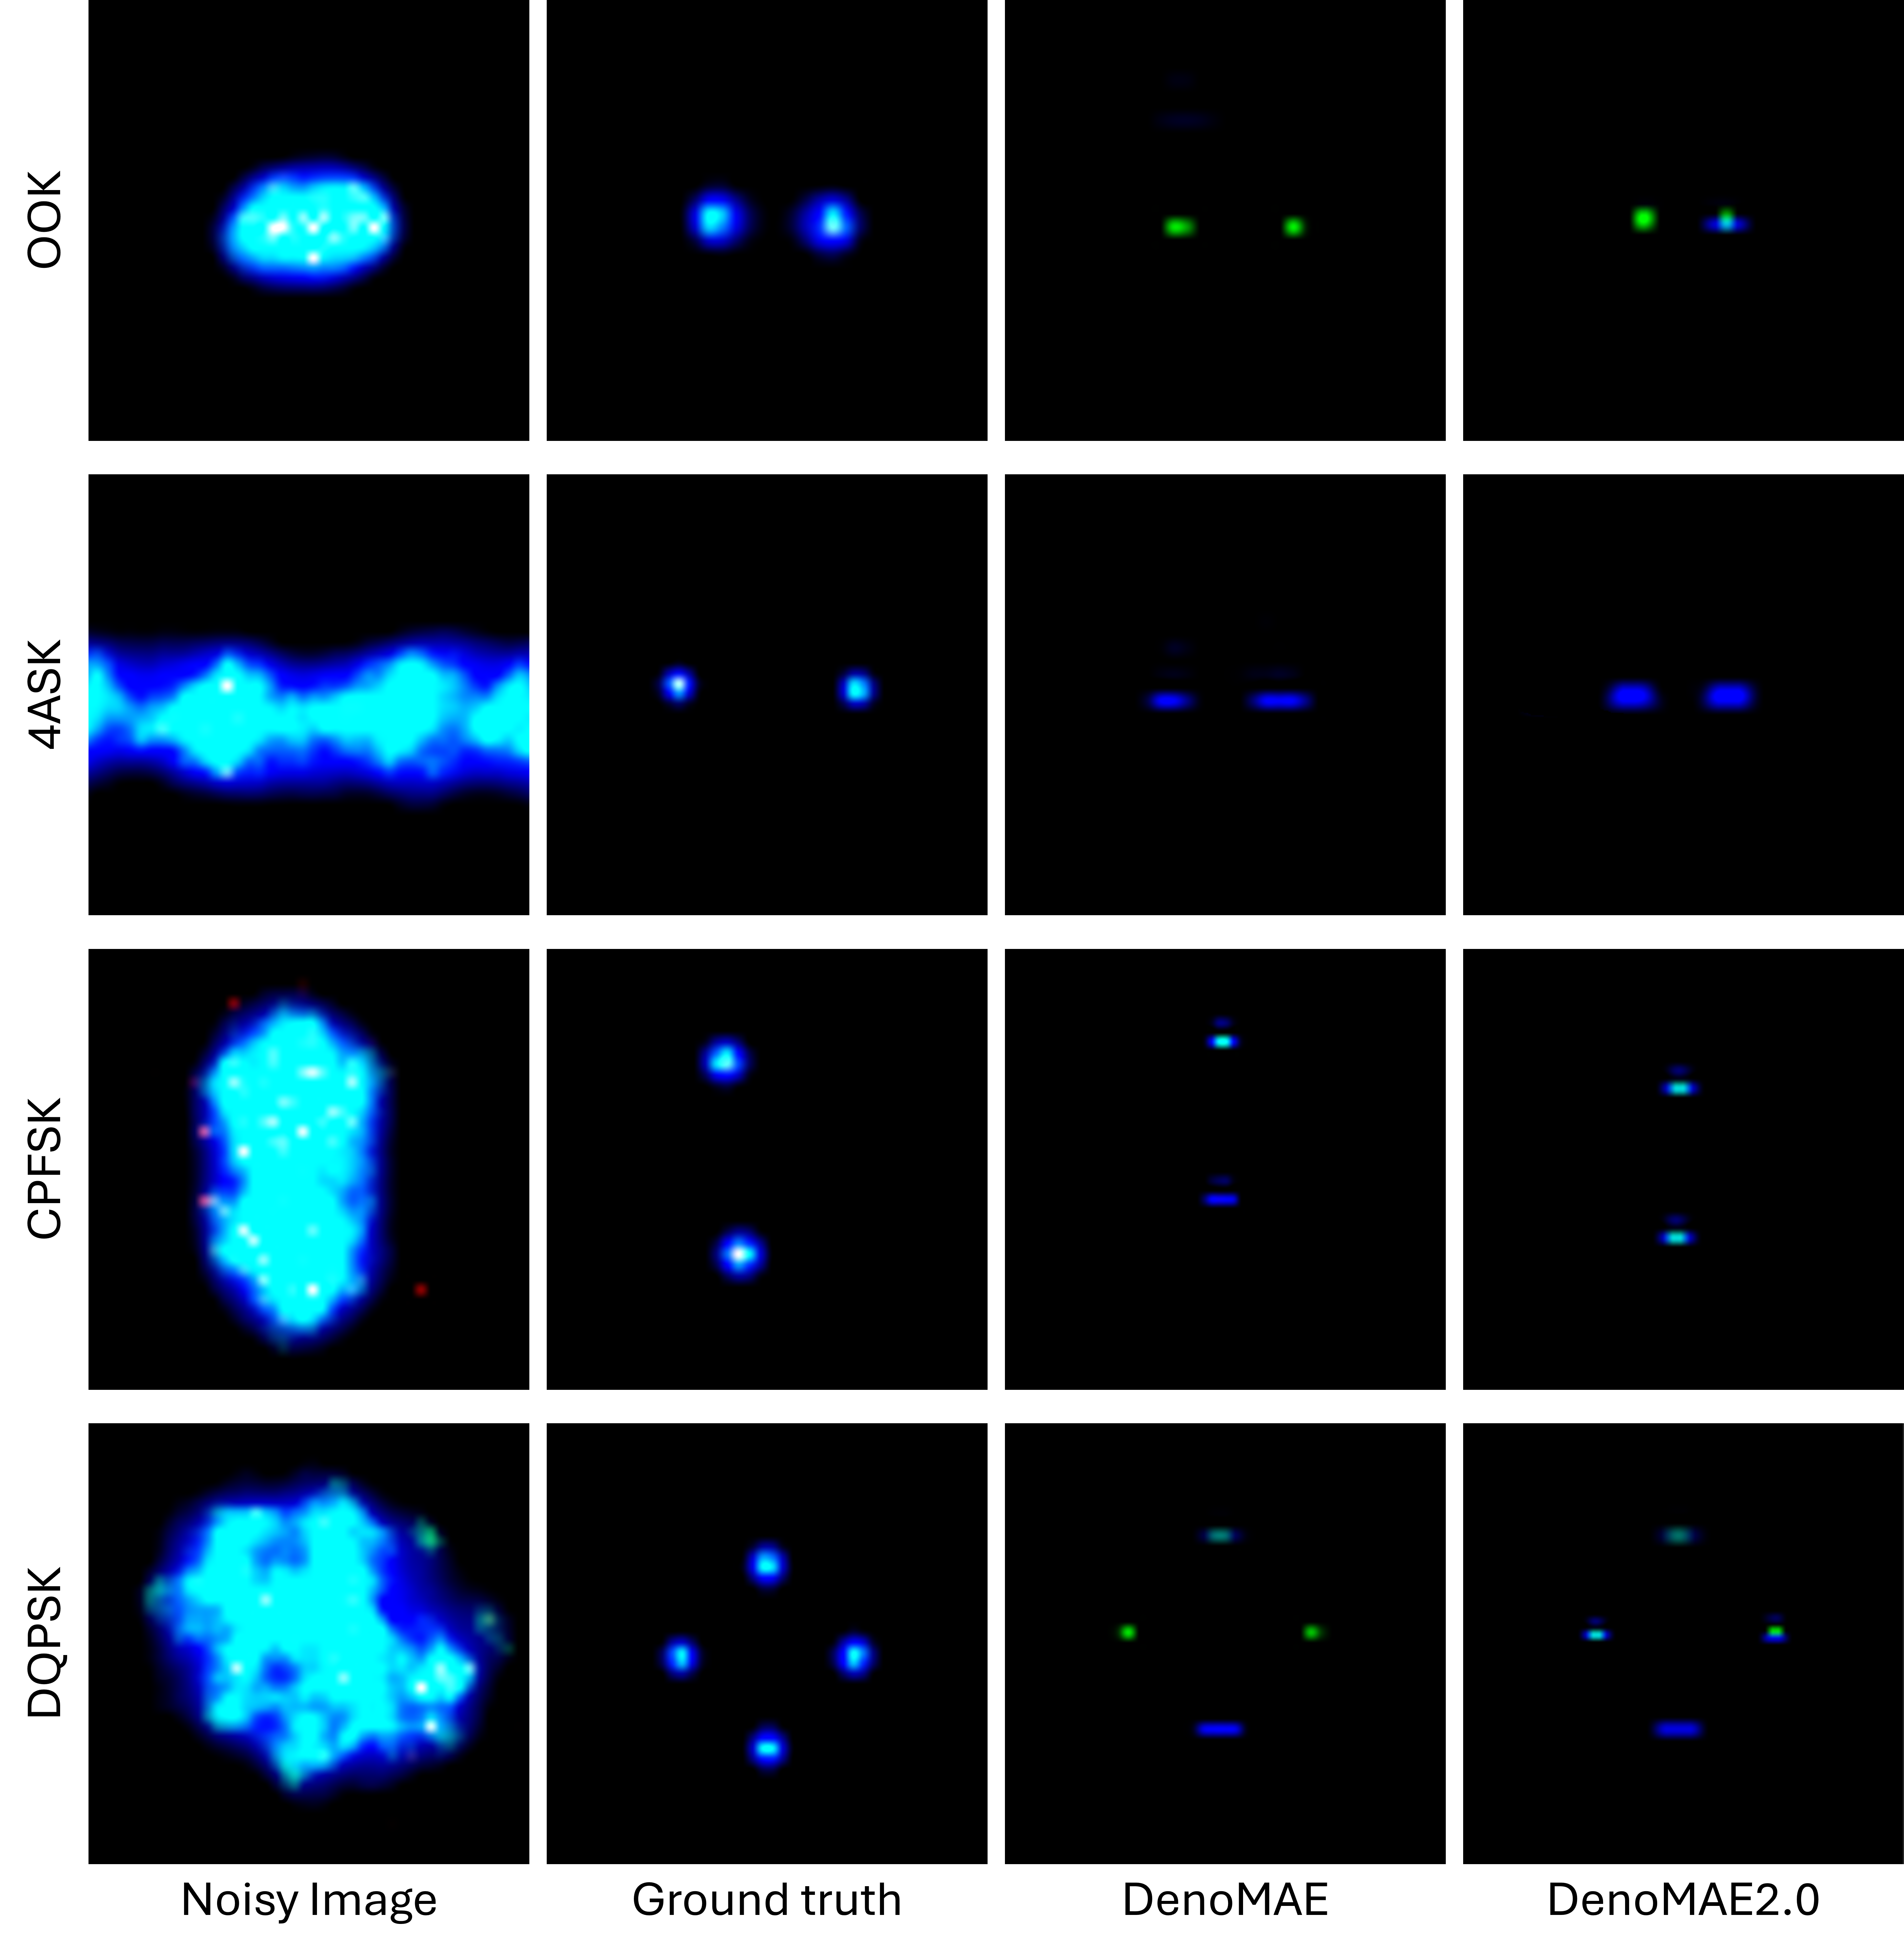
\includegraphics[width=0.9\linewidth]{FIGURES/denomae2/recon.png}
%     \caption{Reconstruction performance comparison between DenoMAE and DenoMAE2.0}
%     \label{fig:recon}
% \end{figure}

% During the pretraining phase, DenoMAE2.0 learns to denoise and reconstruct missing patches, thereby developing robust signal representations. We evaluate this denoising and reconstruction performance both during and after pretraining. Figure \ref{fig:recon} illustrates the effectiveness of DenoMAE2.0 through reconstructed constellation diagrams compared to the original DenoMAE model. DenoMAE2.0 achieves superior noise reduction while preserving critical signal features necessary for accurate modulation classification.

% Table \ref{tab:ssim_psnr_comparison} quantifies these improvements using two standard image quality metrics: structural similarity index (SSIM) and peak signal-to-noise ratio (PSNR). We report the mean SSIM and PSNR scores across all validation images (ten images per class) during pretraining. The results demonstrate that DenoMAE2.0 consistently outperforms the original DenoMAE across all modulation classes. For SSIM, DenoMAE2.0 shows improvements ranging from minor enhancements (0.0004 increase for DQPSK) to substantial gains (0.0315 increase for 4PAM). Similarly, for PSNR, DenoMAE2.0 achieves consistent improvements across all classes, with particularly notable enhancements for GMSK (0.2793 dB increase) and OOK (0.2911 dB increase). These consistent improvements in reconstruction quality metrics directly contribute to the enhanced downstream classification performance of DenoMAE2.0.

% \begin{table*}[htbp]
%     \centering
%     \caption{Quantitative Comparison of Denoising Performance between DenoMAE and DenoMAE2.0.}
%     \label{tab:ssim_psnr_comparison}
%     \renewcommand{\arraystretch}{1.1}
%     \begin{tabular}{ccccc}
%         \hline
%         \multirow{2}{*}{\textbf{Class}} & \multicolumn{2}{c}{\textbf{SSIM}} 
%         & \multicolumn{2}{c}{\textbf{PSNR}} \\ 
%         \cline{2-3} \cline{4-5}
%         & \textbf{DenoMAE} & \textbf{DenoMAE2.0} & \textbf{DenoMAE} & \textbf{DenoMAE2.0} \\ \hline
%         16PAM  & 0.9422 & 0.9464 & 41.6867 & 41.8003 \\
%         4ASK   & 0.9607 & 0.9634 & 42.1780 & 42.3096 \\
%         4PAM   & 0.9328 & 0.9643 & 42.0005 & 42.1061 \\
%         8ASK   & 0.9745 & 0.9813 & 42.8006 & 42.9158 \\
%         CPFSK  & 0.9719 & 0.9738 & 42.3492 & 42.5520 \\
%         DQPSK  & 0.9356 & 0.9360 & 41.8405 & 41.9223 \\
%         GFSK   & 0.9677 & 0.9681 & 42.0733 & 42.1021 \\
%         GMSK   & 0.8749 & 0.8771 & 39.9367 & 40.2160 \\
%         OOK    & 0.9586 & 0.9674 & 42.3674 & 42.6585 \\
%         OQPSK  & 0.9129 & 0.9204 & 41.0052 & 41.1172 \\ \hline
%     \end{tabular}
% \end{table*}

% \subsubsection{Latent Space Visualization with TSNE}

% In Figure~\ref{fig:tsne}, we visualize the latent representations of DenoMAE and DenoMAE2.0 using t-distributed stochastic neighbor embedding (t-SNE)~\cite{van2008visualizing}. The plots (left two) reveal that DenoMAE2.0 produces more accurate and distinct clusters than DenoMAE, indicating superior feature separation and representation learning. Specifically, in DenoMAE, classes 0, 3, and 9 contain more separated clusters within the same class. In contrast, DenoMAE2.0 exhibits more distinct clusters for these classes.

% This enhanced clustering is particularly evident in the masked samples (right two plots), where we mask out a significant portion (75\%) of the images. Masking typically makes distinct cluster formation more challenging. However, DenoMAE2.0 achieves clearer boundaries between classes, suggesting improved robustness and generalization capabilities. In DenoMAE, classes 0, 3, and 9 achieve somewhat distinct clusters, with a few samples overlapping in other clusters. In DenoMAE2.0, classes 0, 3, 6, 7, 8, and 9 show better-separated clusters, indicating enhanced feature learning and representation.

% However, in all the plots, classes 1 and 2 entirely overlap with each other, indicating that the model struggles to distinguish between these two classes. This is a common issue in modulation classification, as some classes are very similar to each other.

% \begin{figure*}
%     \centering
%     \subfloat{%
%        \includegraphics[trim=1cm 1cm 1cm 1cm,clip,
%        width=0.25\linewidth]{FIGURES/denomae2/denoMAE_no_mask.png}}
%     \hfill
%     \subfloat{%
%         \includegraphics[trim=1cm 1cm 1cm 1cm,clip,
%         width=0.25\linewidth]{FIGURES/denomae2/denoMAE2_no_mask.png}}
%     \hfill
%     \subfloat{%
%         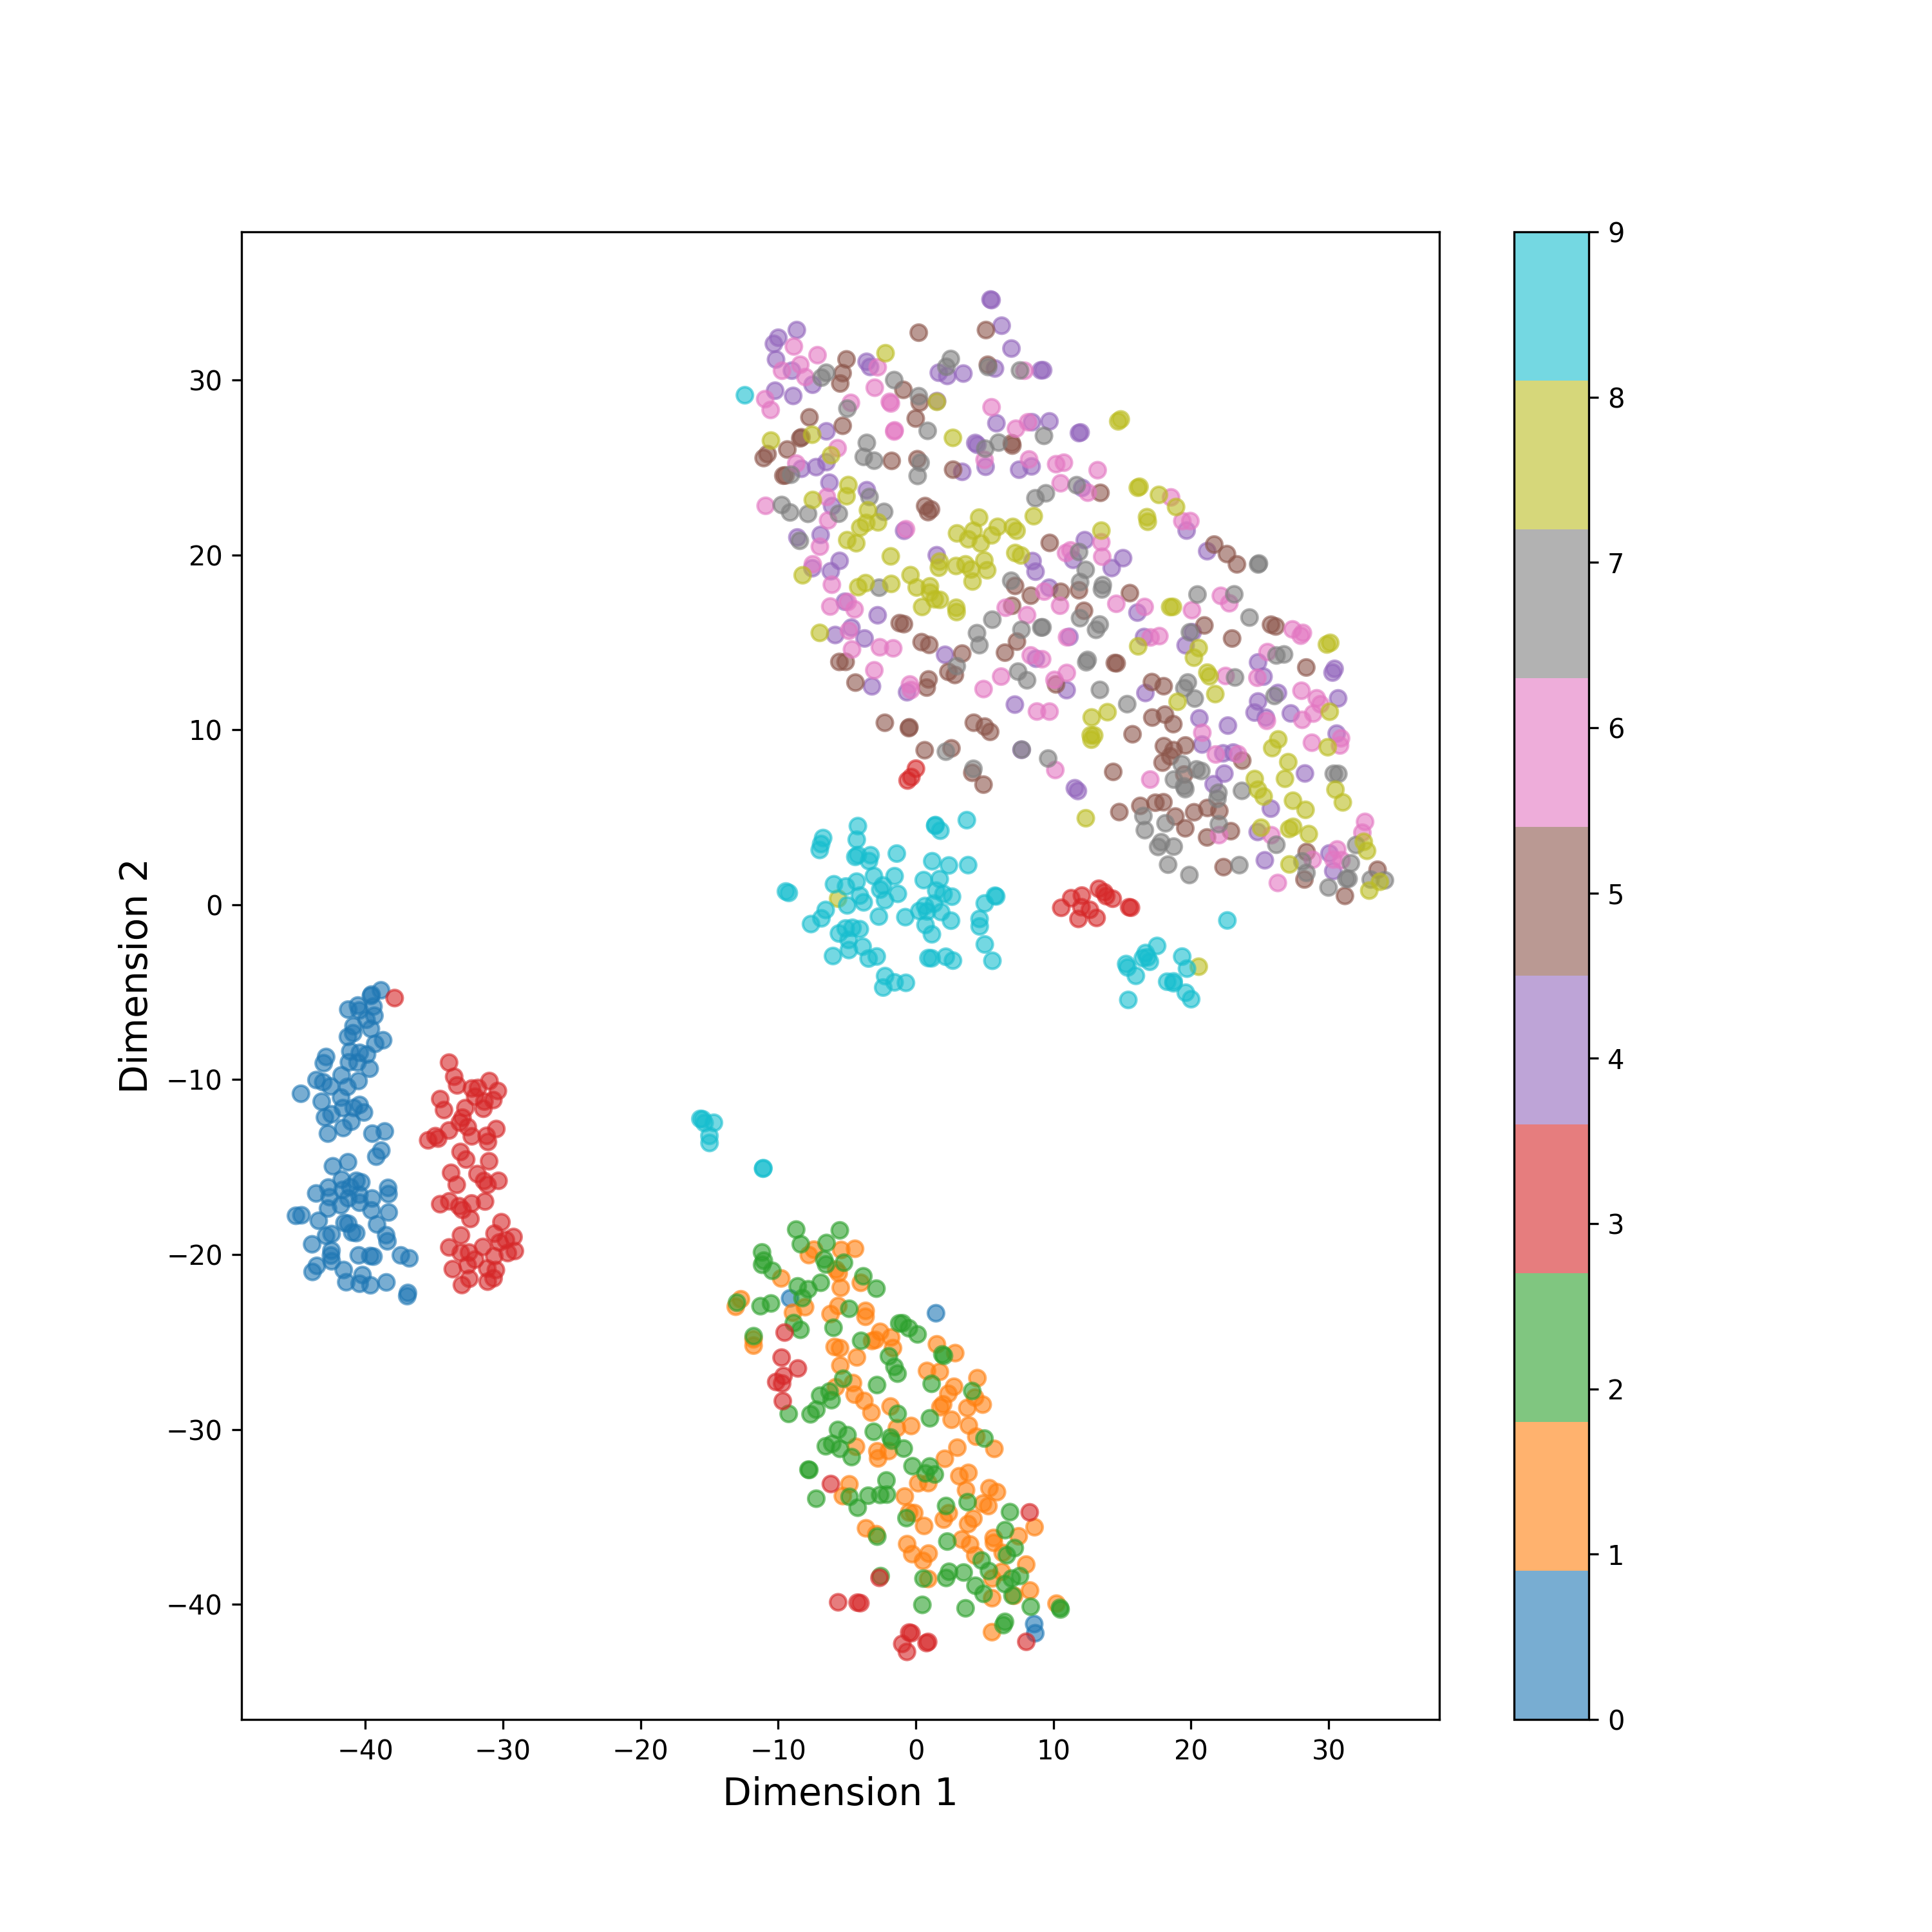
\includegraphics[trim=1cm 1cm 1cm 1cm,clip,
%         width=0.25\linewidth]{FIGURES/denomae2/denoMAE_mask.png}}
%     \hfill
%     \subfloat{%
%         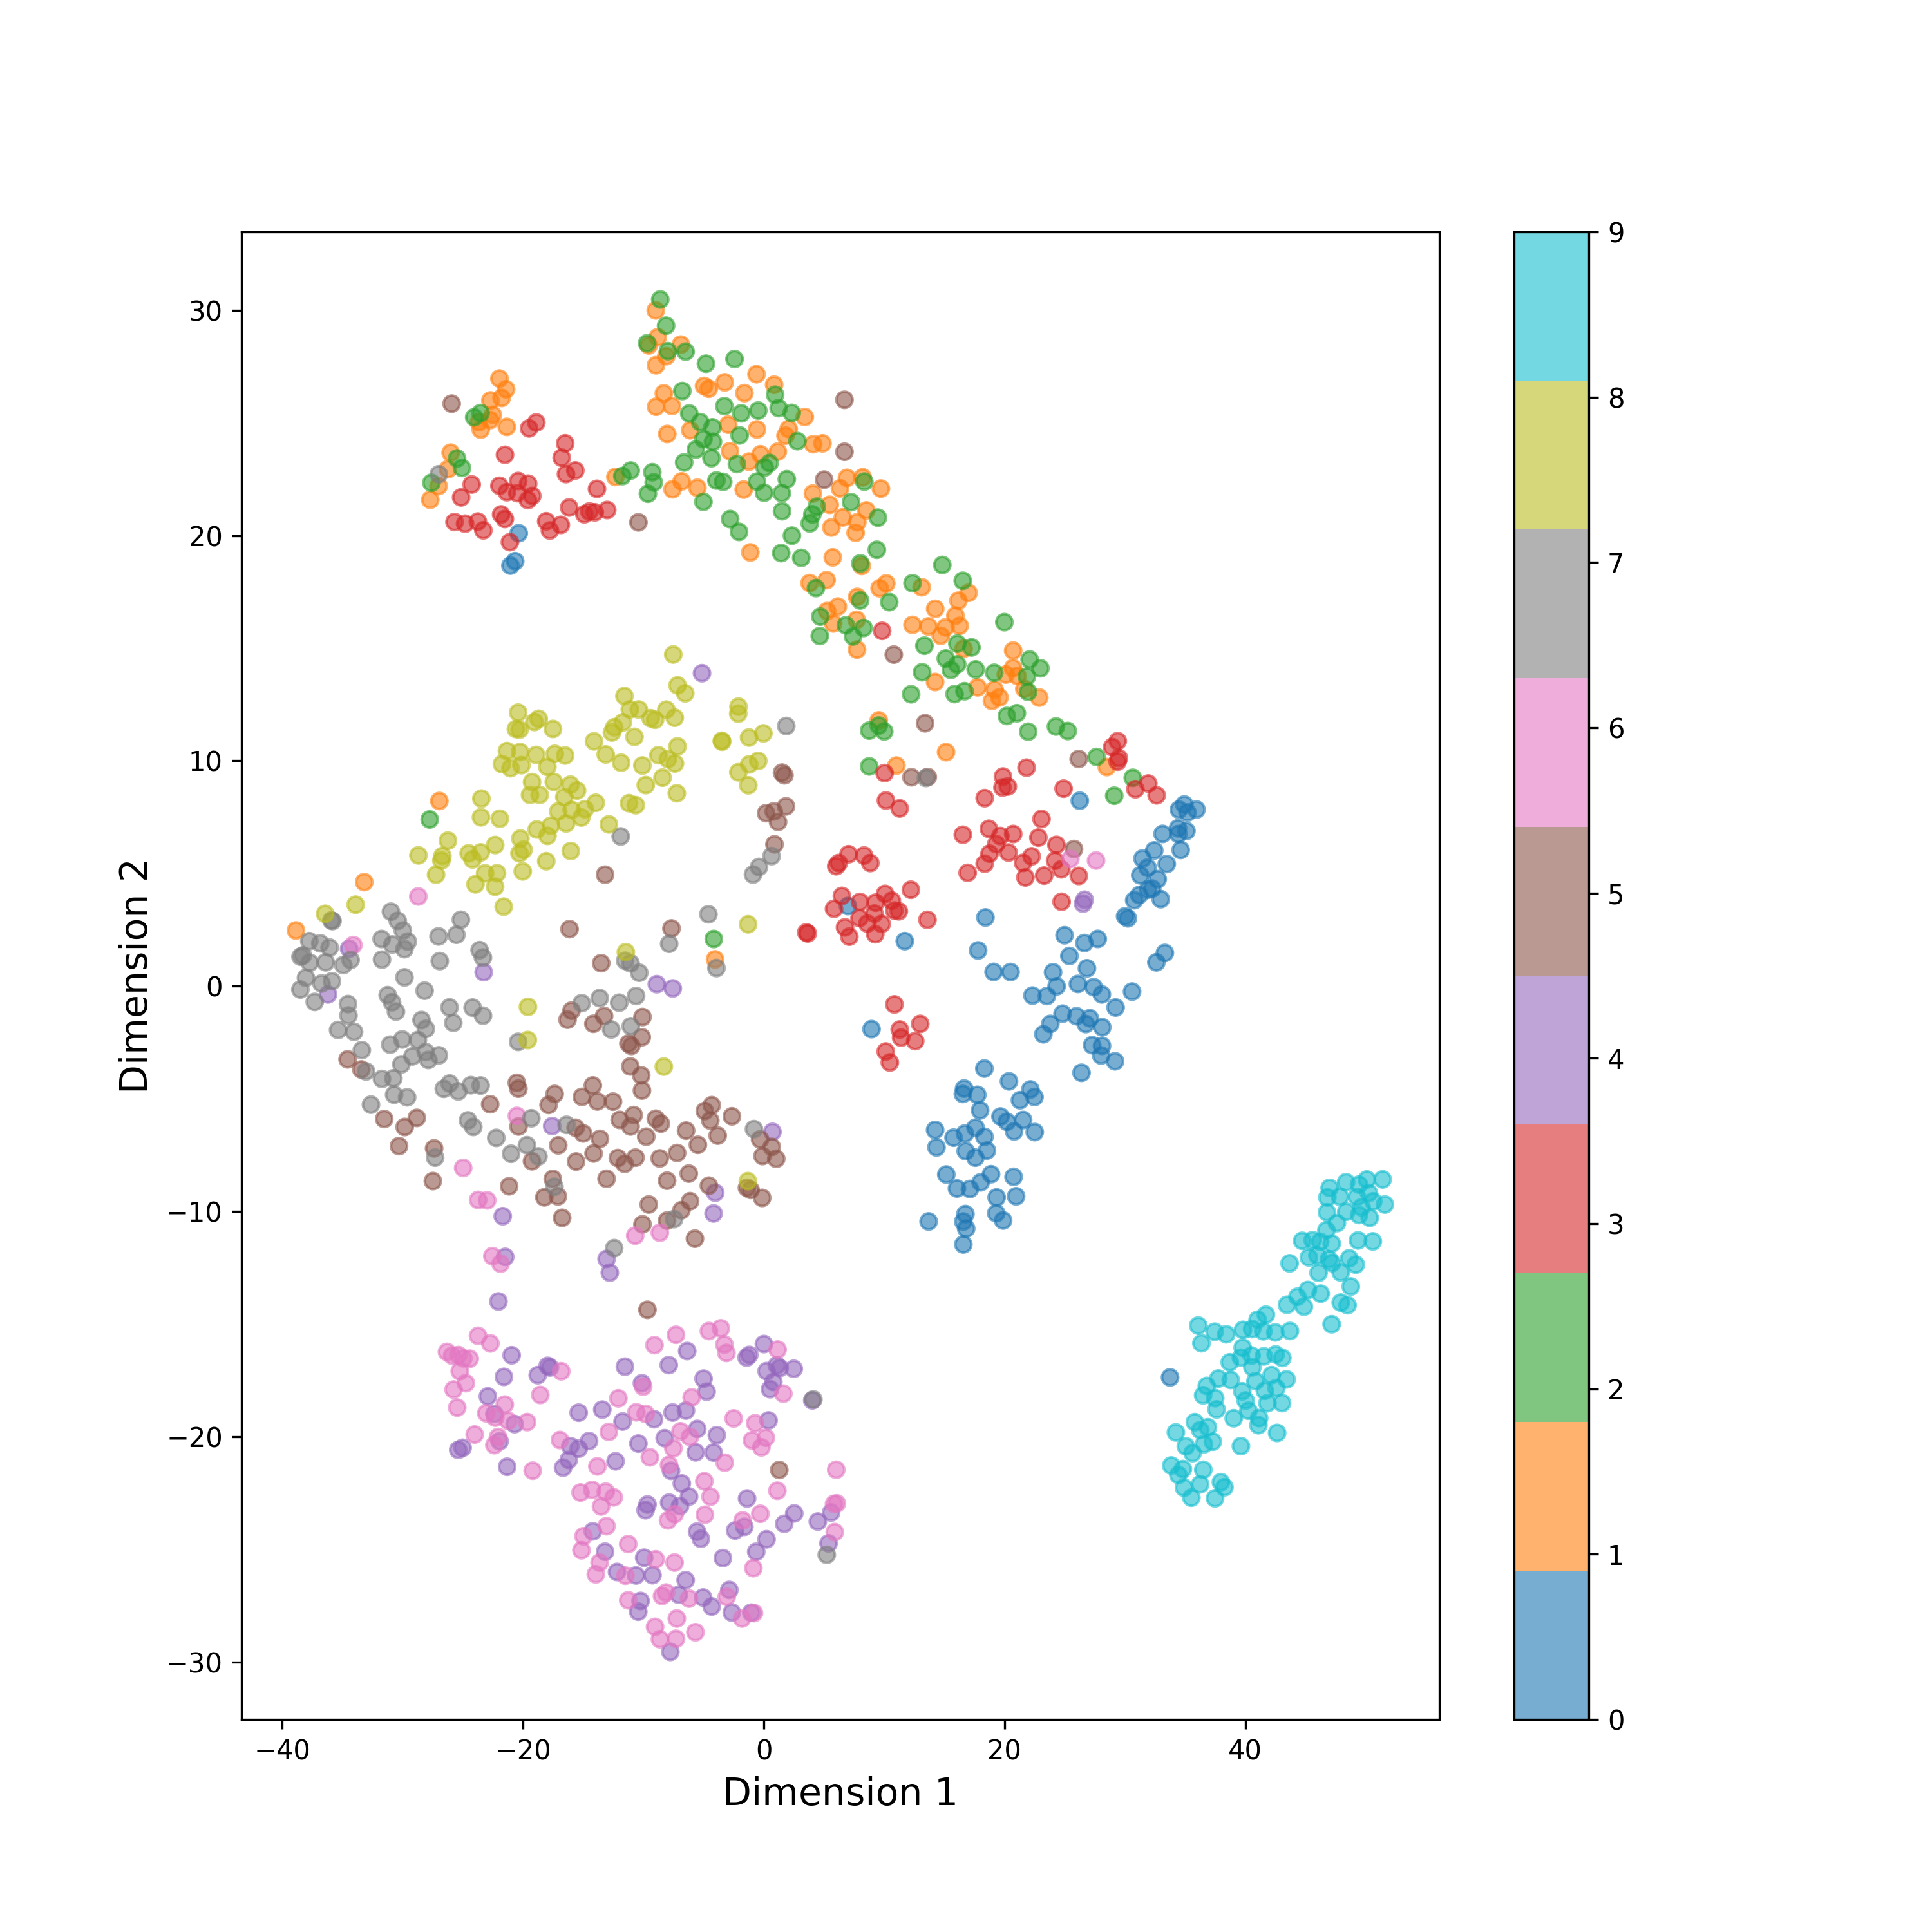
\includegraphics[trim=1cm 1cm 1cm 1cm,clip,
%         width=0.25\linewidth]{FIGURES/denomae2/denoMAE2_mask.png}}
%     \caption{Latent representation visualization using t-SNE. From left to right: (1) DenoMAE without masking, (2) DenoMAE2.0 without masking, (3) DenoMAE with 75\% masking, and (4) DenoMAE2.0 with 75\% masking.}
%     \label{fig:tsne} 
% \end{figure*}

% \subsubsection{Finetuning Accuracy}

% After pretraining, we transfer the learned representations to the downstream classification task and compare DenoMAE2.0 with state-of-the-art models. As shown in Table \ref{tab:example}, when finetuned on the downstream task, DenoMAE2.0 achieves the highest test accuracy of 82.40\% among all compared methods. This represents a significant improvement over the baseline ViT (79.90\%) and other representation learning approaches including DEiT (81.20\%), MoCov3 (81.00\%), BEiT (80.40\%), MAE (80.10\%), and the original DenoMAE (81.30\%). The consistent performance advantage demonstrates that DenoMAE2.0's enhanced denoising strategy learns more effective representations during pretraining that transfers well to the downstream classification task.

% \begin{table}[htbp]
%     \centering
%     \caption{Downstream classification accuracy for different models}
%     \begin{tabular}{cc}
%         \hline
%         \textbf{Method} & \textbf{Test accuracy (\%)} \\ \hline
%         ViT \cite{dosovitskiy2020image} & 79.90 \\ 
%         DEiT \cite{touvron2021training} & 81.20 \\ 
%         MoCov3 \cite{xie2021self} & 81.00 \\ 
%         BEiT \cite{bao2021beit} & 80.40 \\
%         MAE \cite{he2022masked} &  80.10 \\ 
%         DenoMAE \cite{faysal2025denomae} &  81.30 \\
%         DenoMAE2.0  (\textbf{Ours}) &  \textbf{82.40} \\ \hline
%     \end{tabular}
%     \label{tab:example}
% \end{table}

% \subsubsection{Confusion Matrix}

% Figure~\ref{fig:confusion} presents confusion matrices visualizing the per-class performance of both DenoMAE and DenoMAE2.0. The diagonal elements indicate correct classifications, while off-diagonal elements show misclassifications. Both models demonstrate perfect classification accuracy (100\%) for several modulation types, specifically 16PAM, 4ASK, 8ASK, DQPSK, GMSK, OOK, and OQPSK. 

% However, persistent classification challenges are evident between 4ASK and 4PAM, where both models show significant confusion with 50\% accuracy for each class and 50\% misclassification between them. This symmetric confusion pattern suggests inherent signal similarities between these amplitude modulation schemes that remain difficult to distinguish even with our enhanced architecture. Notably, this confusion pattern directly aligns with observations from the t-SNE analysis, where classes 1 and 2 show complete overlap in the latent space visualization, further confirming the inherent similarity in signal characteristics between these modulation types.

% Additionally, both models struggle with differentiating between CPFSK and GFSK, though DenoMAE2.0 shows modest improvement in CPFSK recognition (70\% accuracy compared to 63\% in DenoMAE). Despite this improvement, GFSK classification remains challenging with DenoMAE2.0 achieving only 54\% accuracy (compared to 52\% in DenoMAE), with most misclassifications assigning GFSK signals to the CPFSK class. This confusion pattern aligns with the theoretical similarity between these frequency shift keying techniques, as GFSK is essentially CPFSK with additional Gaussian filtering. These consistent patterns across both model versions indicate fundamental signal similarities that present intrinsic classification challenges rather than model limitations.

% \begin{figure}[htbp]
%     \centering
%     \subfloat{%
%         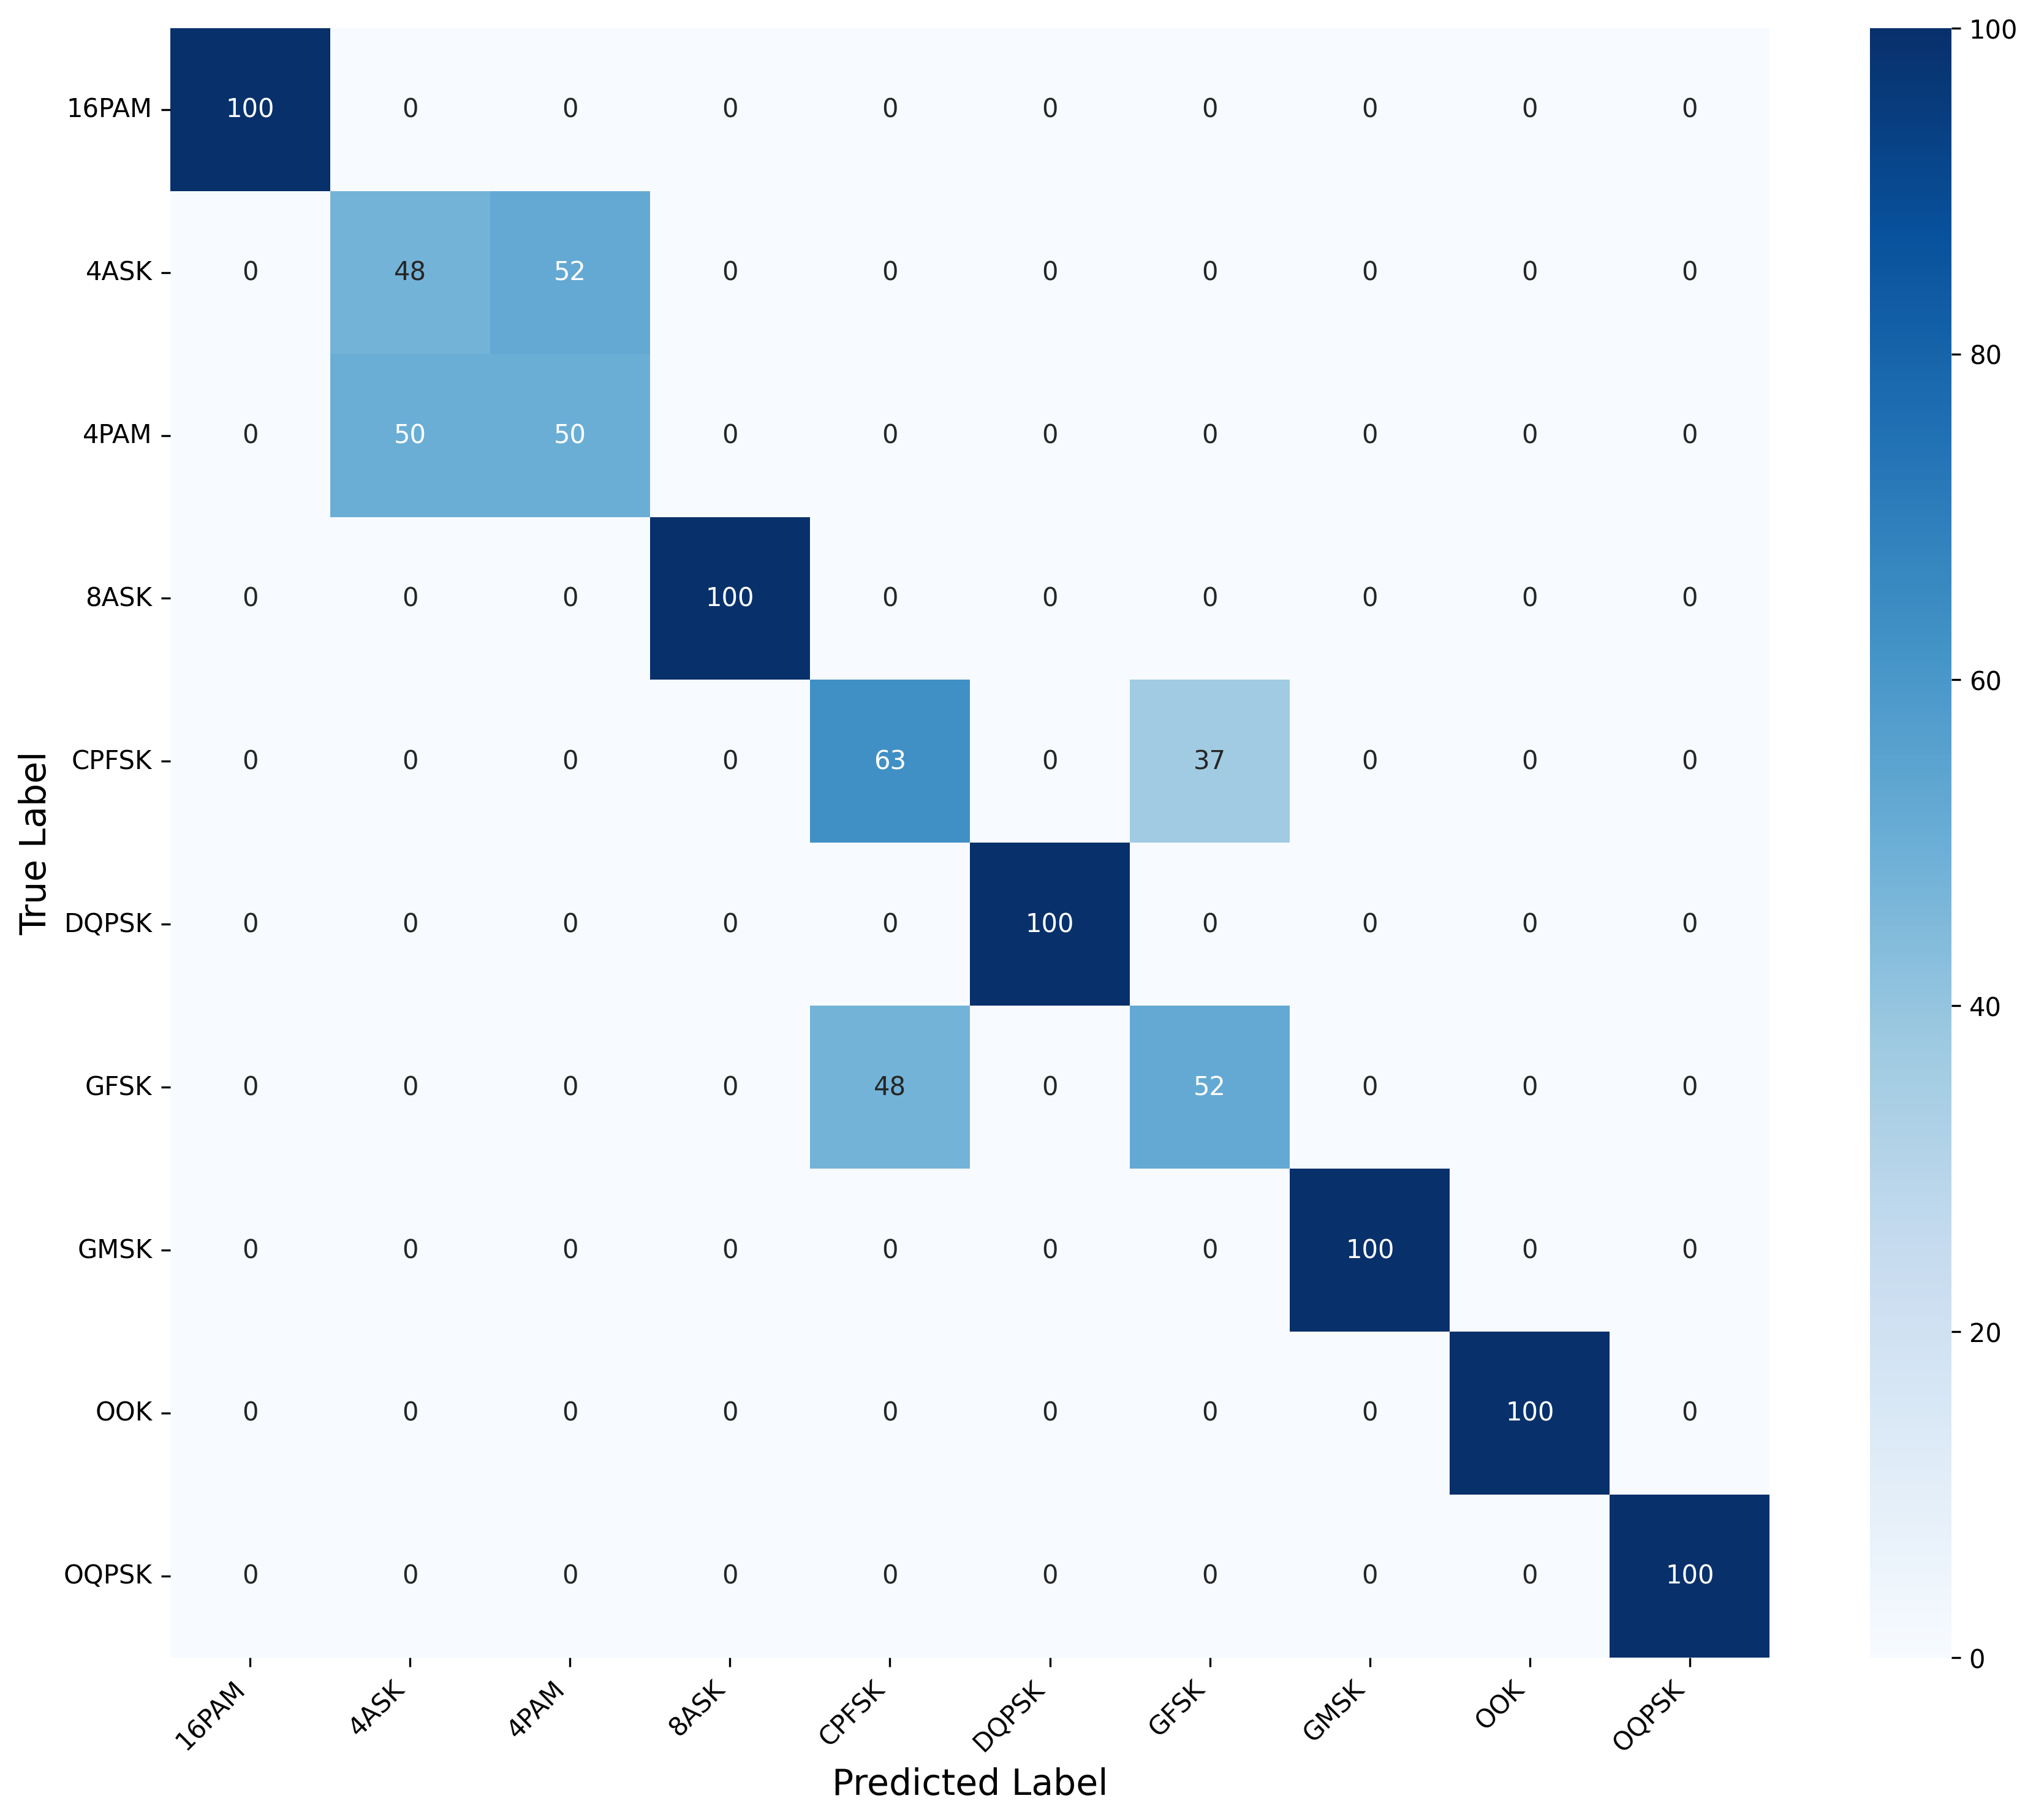
\includegraphics[width=0.48\linewidth]{FIGURES/denomae2/deno_cm.png}}
%     \hfill
%     \subfloat{%
%         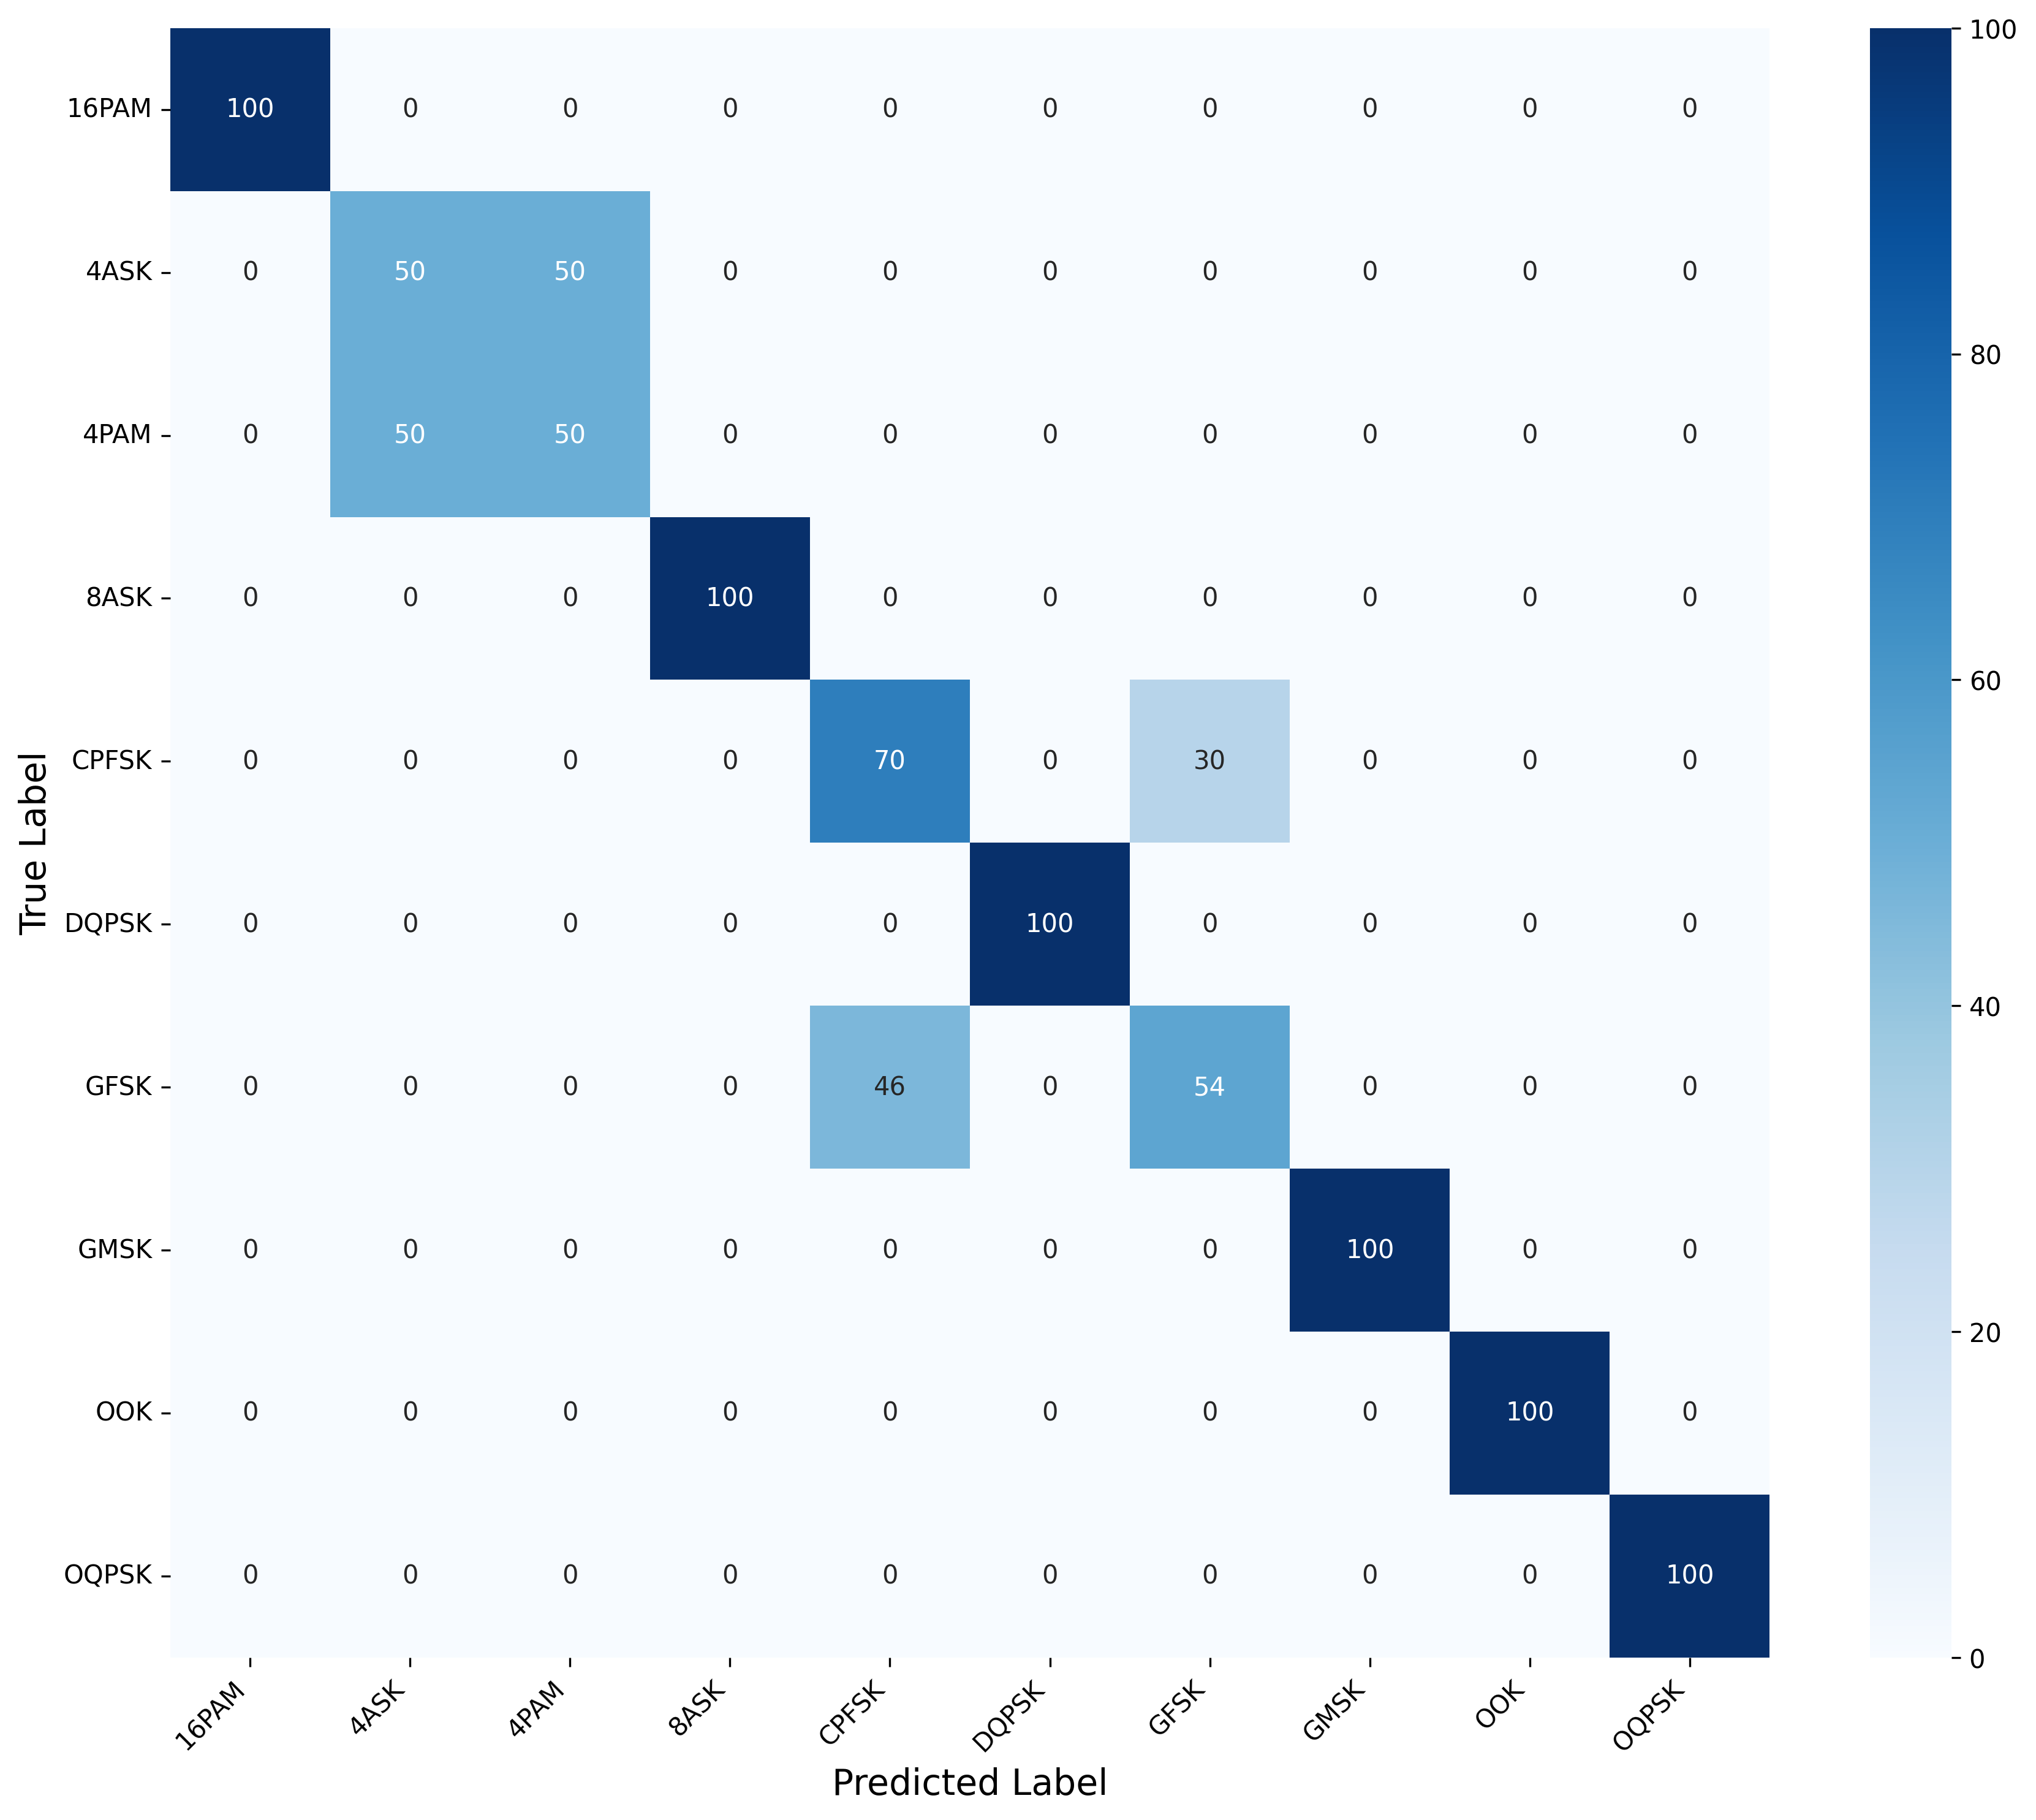
\includegraphics[width=0.48\linewidth]{FIGURES/denomae2/deno2_cm.png}}
%     \caption{Confusion matrices for downstream classification. Left: DenoMAE, Right: DenoMAE2.0} 
%     \label{fig:confusion}
% \end{figure}


% \subsubsection{Performance on Number of Epochs}

% \begin{figure}[htbp]
%     \centering
%     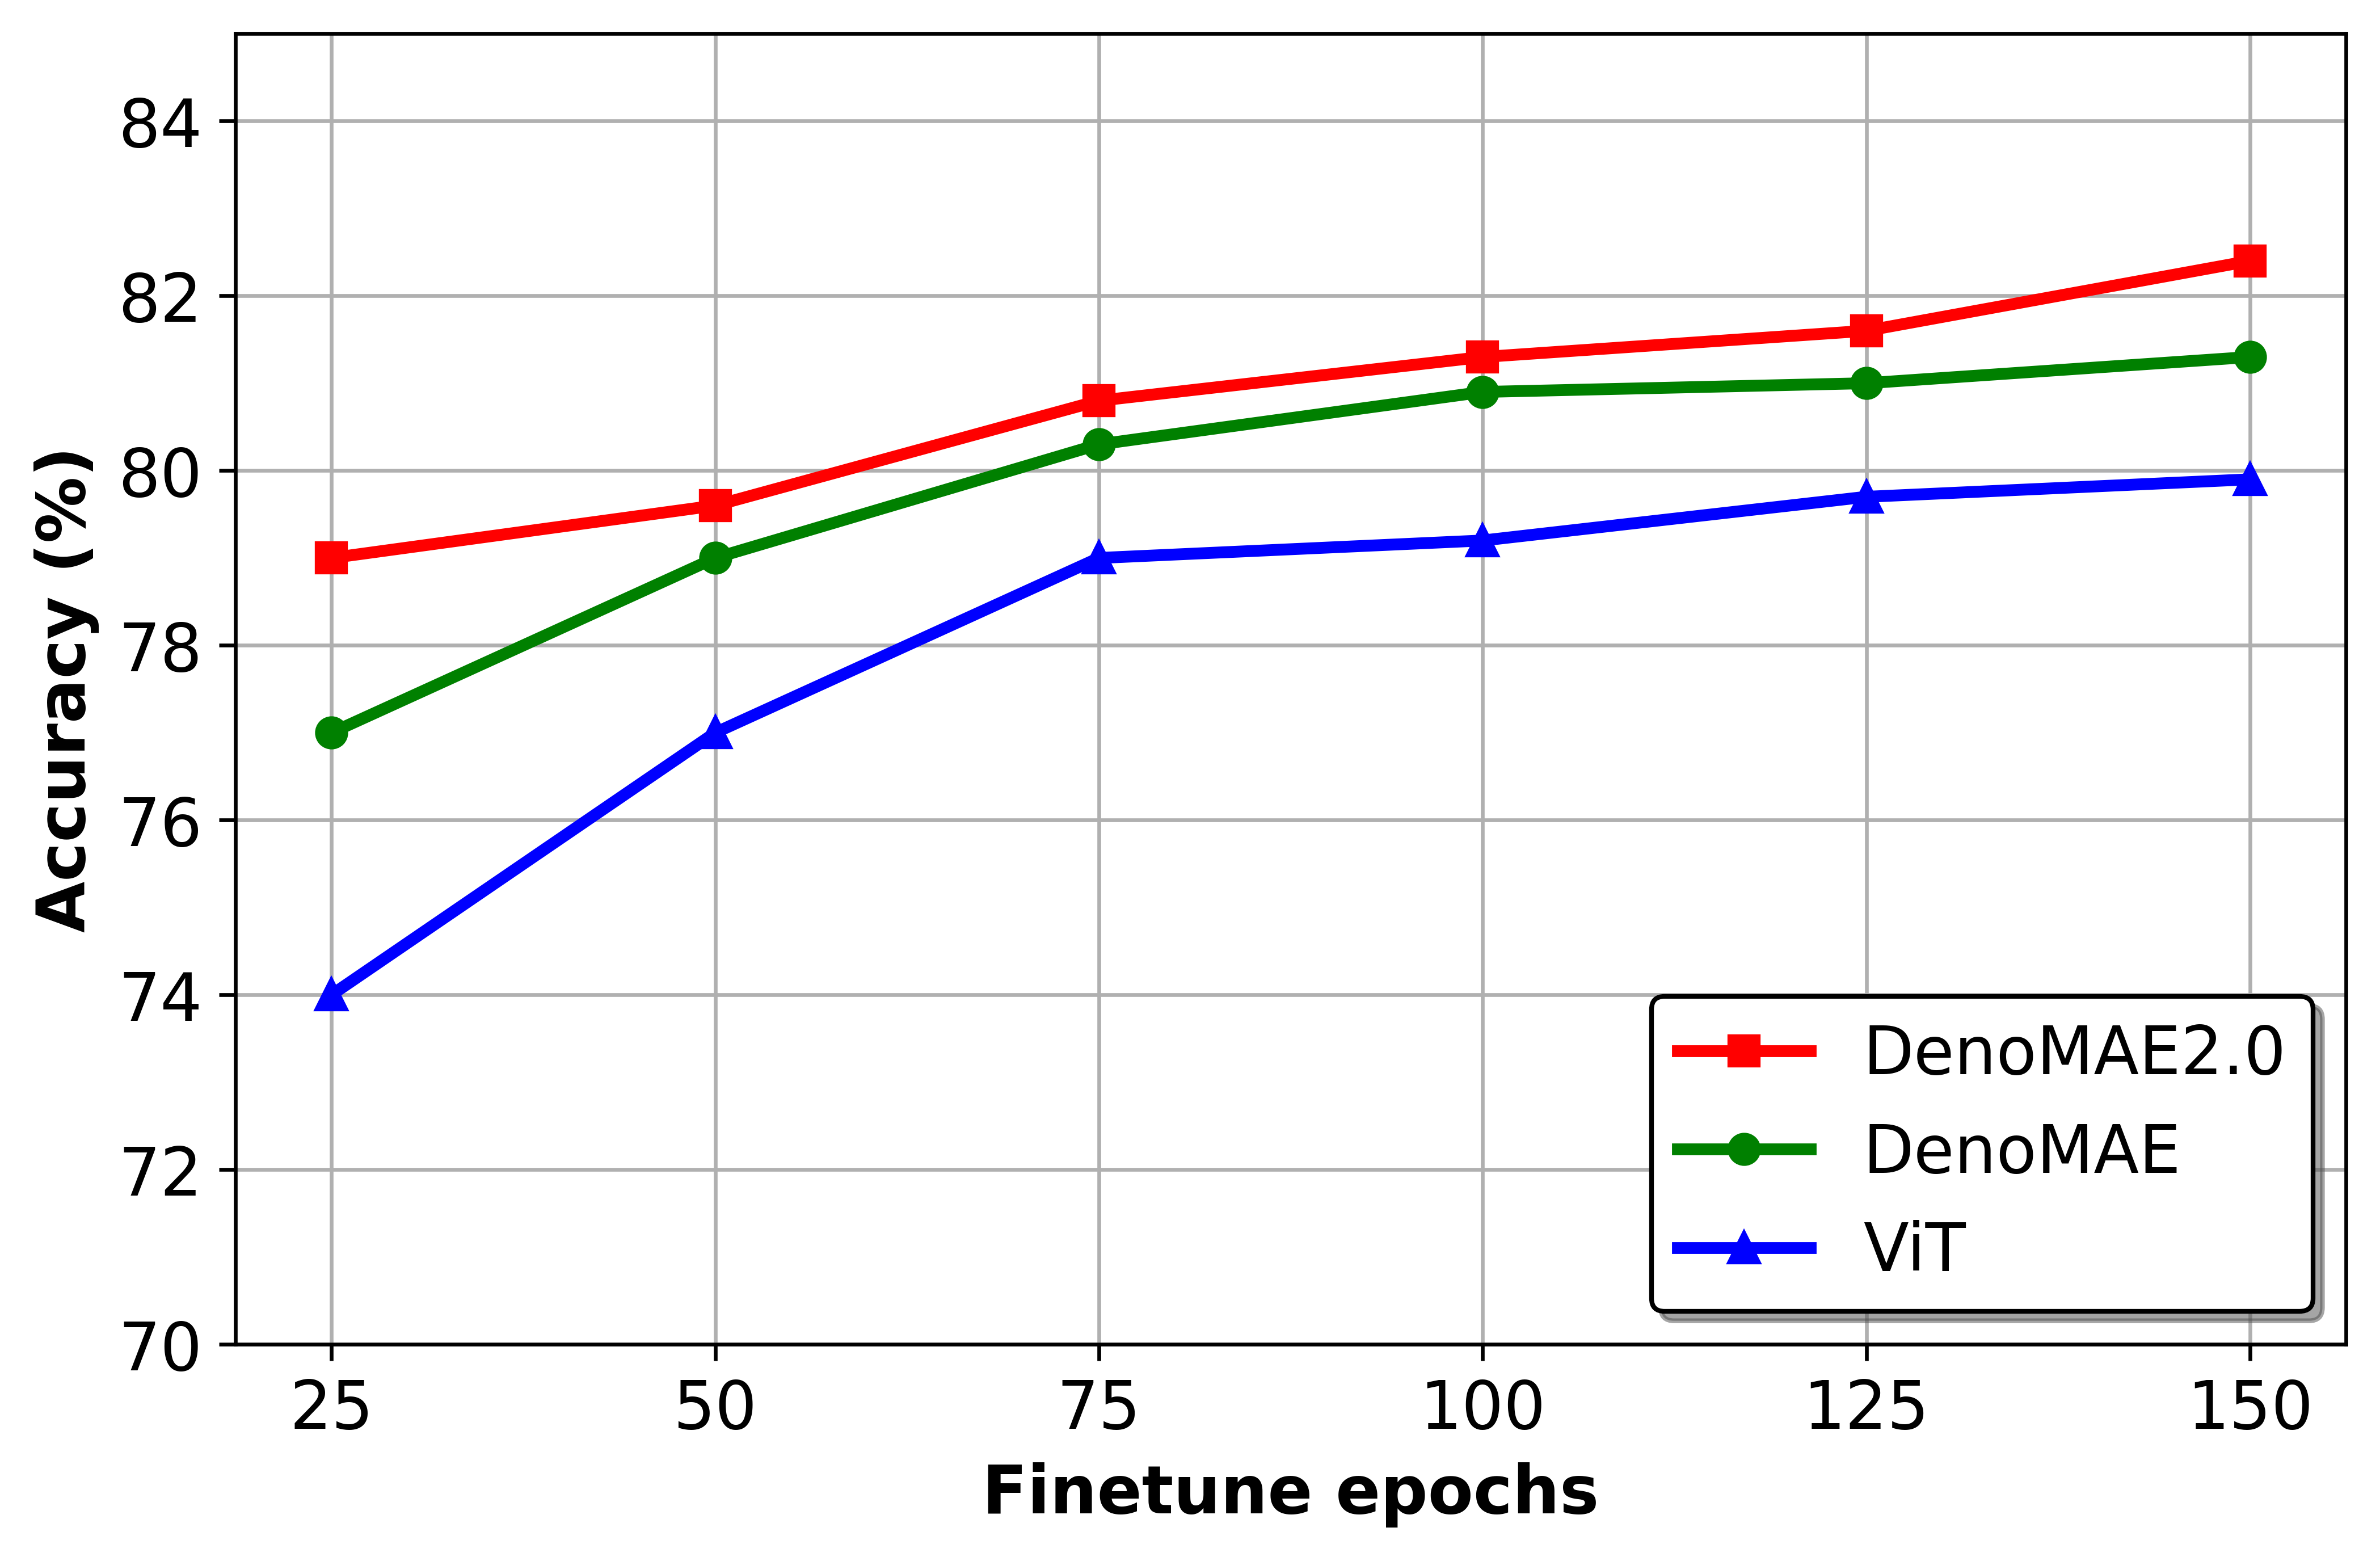
\includegraphics[width=0.9\linewidth]{FIGURES/denomae2/finetune_epoch.png}
%     \caption{Finetuning performance improvement for  different epochs}
%     \label{fig:epoch}
% \end{figure}

% Figure~\ref{fig:epoch} illustrates the finetuning performance across different epochs. The plot shows a steady improvement in model accuracy as the number of epochs increases, with DenoMAE2.0 consistently outperforming baseline methods. DenoMAE achieves higher accuracy than ViT continuously. On the other hand, although the gap between DenoMAE and ViT is larger than DenoMAE and DenoMAE2.0, DenoMAE2.0 always obtains better accuracy than DenoMAE.

% \subsubsection{Performance Across Different SNRs}

% The SNR performance plot demonstrates robust classification accuracy across various SNRs ranging from -10 dB to 10 dB. As the SNR values increases all the methods perform better and when the SNR is low the performance degrades. ViT, which has no pertaining phase, presumably obntains the lowest performance in all cases. MAE, which pretrains on modulation signals but has no denoising capability, obtains a slight higher accuracy than ViT. DenoMAE obtains higher accuracy than MAE in most cases however for SNE of 2 and 3 we observe that MAE obtains a higher accuracy. On the other hand, DenoMAE2.0 outperforms all the methods for all the SNRs.  Noteably, all the methods lose significant accuracy for snr lower than -2 dB. However, DenoMAE2.0 maintains comparatively robust performance down to -7 dB, demonstrating its enhanced resilience to noise.

% \begin{figure}[htbp]
%     \centering
%     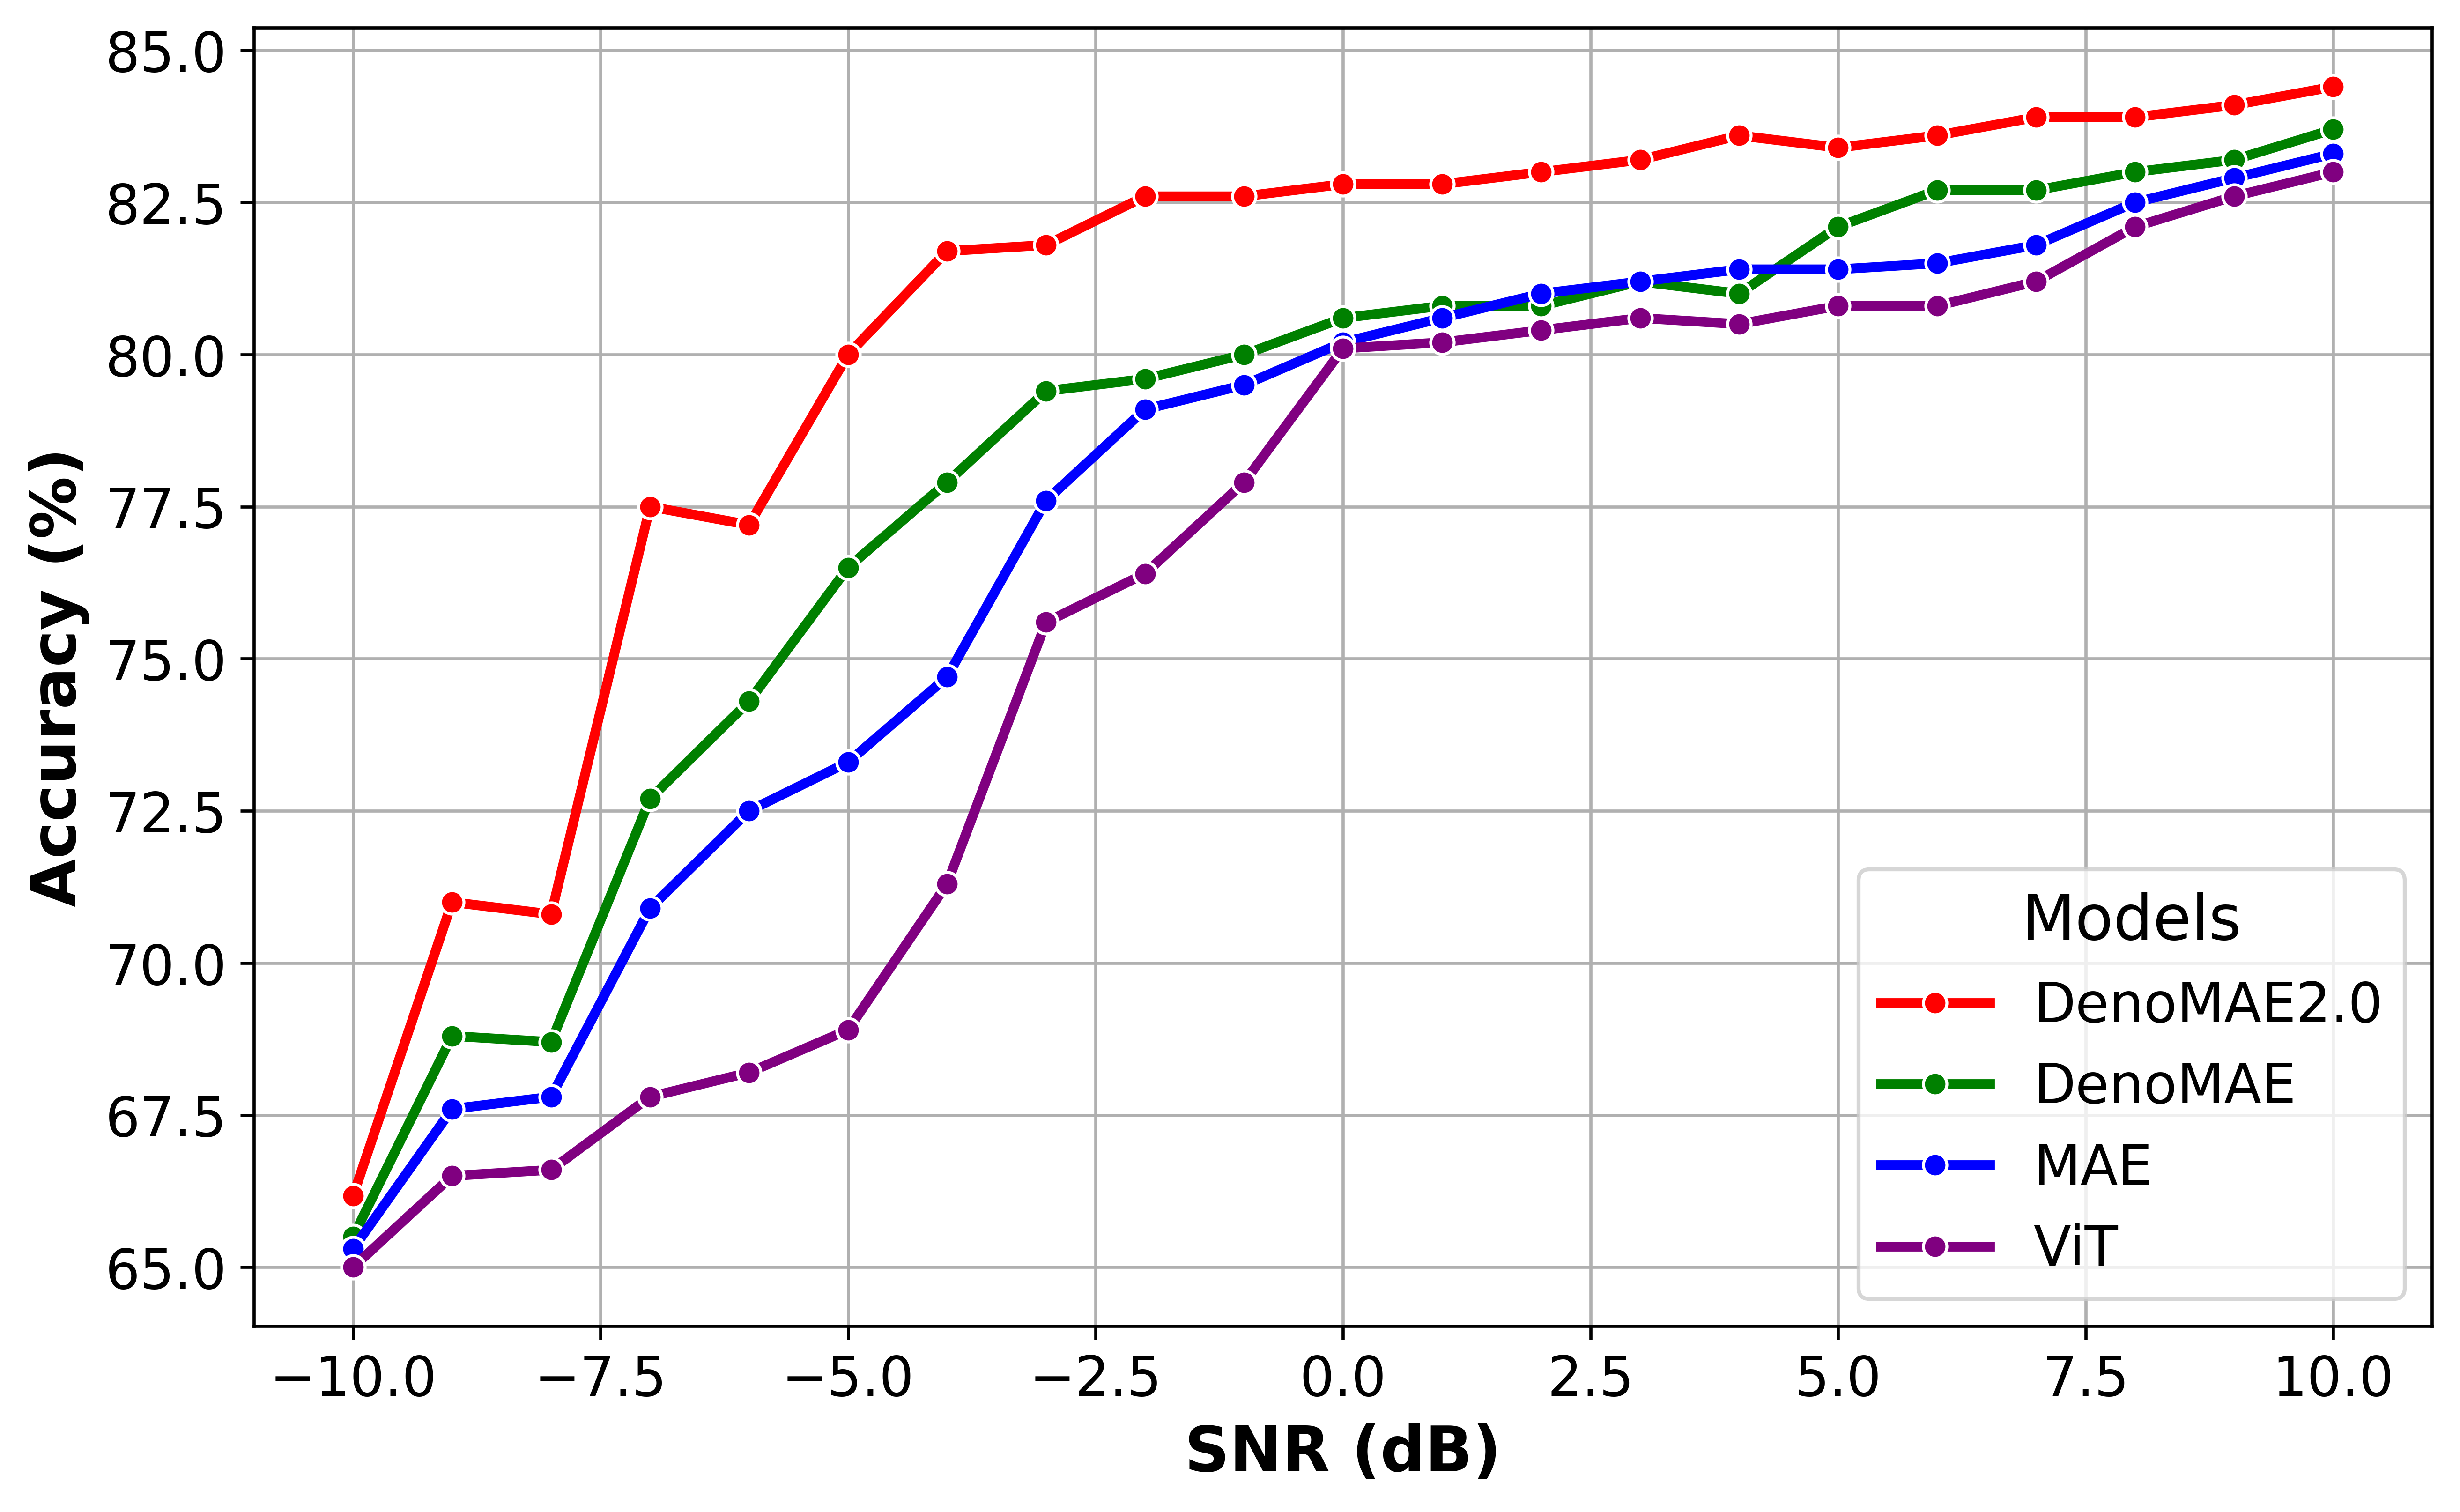
\includegraphics[width=\linewidth]{FIGURES/denomae2/SNR_Accuracy_Plot.png}
%     \caption{Accuracy comparison across different SNRs}
%     \label{fig:snr_acc}
% \end{figure}

% \subsection{Comparison with Other AMC Methods}

% Table~\ref{tab:compare} presents a comprehensive comparison between DenoMAE2.0 and other state-of-the-art modulation classification methods. AlexNet achieved 82.8\% accuracy with 8 classes at 2dB SNR using a large dataset of 800,000 samples. NMformer reported 71.6\% accuracy across 10 classes with SNR ranging from 0.5 to 4.5dB using 106,800 samples. CNN-AMC and DL-GRF showed relatively lower performance with 50.40\% and 59\% accuracy respectively, though they were tested under different conditions. The original DenoMAE achieved 81.3\% accuracy across 10 classes with SNR ranging from 0 to 10dB. Our proposed DenoMAE2.0 demonstrates superior performance with 82.4\% accuracy under similar conditions, using only 10,000 samples for pretraining and 1,000 samples for fine-tuning, indicating improved efficiency in both performance and data utilization.

% \begin{table}[htbp]
%     \centering
%     \caption{Comparison of DenoMAE2.0 with other modulation classification methods}
%     \label{tab:compare}
%     \begin{tabular}{cccccc}
%     \toprule
%     \multirow{2}{*}{\textbf{Methods}} & \multicolumn{2}{c}{\textbf{Number of samples}} & \multirow{2}{*}{\textbf{SNR (dB)}} & \multirow{2}{*}{\textbf{\# Classes}} & \multirow{2}{*}{\textbf{Accuracy (\%)}} \\ 
%     \cmidrule(lr){2-3}
%      & \textbf{Pretraining} & \textbf{Fine-tuning} & & \\ \midrule
    
%     AlexNet \cite{peng2018modulation}     & 800,000 (train) & 8,000 (test)   & 2         & 8  & 82.8  \\
%     NMformer \cite{faysal2024nmformer}    & 106,800         & 3,000          & 0.5–4.5   & 10 & 71.6  \\
%     CNN-AMC \cite{meng2018automatic}      & 79,200          & 228,060        & –6        & 4  & 50.4  \\
%     DL-GRF \cite{sun2022automatic}        & 2,000 (train)   & 200 (test)     & 0         & 4  & 59    \\
%     DenoMAE \cite{faysal2025denomae}      & 10,000          & 1,000          & 0–10      & 10 & 81.3  \\
%     \textbf{DenoMAE2.0 (Ours)}            & 10,000          & 1,000          & 0–10      & 10 & \textbf{82.4} \\
    
%     \bottomrule
%     \end{tabular}
% \end{table}

% \subsection{Ablation Study}

% In this section, we analyze the impact of various components on the performance of our model.

% \subsubsection{Effect of the Loss Function}

% We conducted experiments to evaluate the contribution of different loss components in our model. As shown in Table~\ref{tab:loss}, we analyzed three configurations: using only reconstruction loss, only classification loss, and combining both losses. The results demonstrate that while reconstruction loss alone achieves reasonable performance (81.30\%), classification loss by itself underperforms (69.80\%). However, combining both losses yields the best results (82.40\%), suggesting that the joint optimization of reconstruction and classification objectives leads to more robust feature learning and better overall performance.

% \begin{table}[htbp]
%     \centering
%     \caption{Accuracy for different loss configurations}
%     \begin{tabular}{ccc}
%         \toprule
%         Reconstruction Loss & Classification Loss & Accuracy (\%) \\
%         \midrule
%         \ding{51} &     & 81.30 \\
%                  & \ding{51} & 69.80 \\
%         \ding{51} & \ding{51} & 82.40 \\
%         \bottomrule
%     \end{tabular}
%     \label{tab:loss}
% \end{table}

% \subsubsection{Effect of Auxiliary Loss Weights}

% We conducted experiments to analyze the impact of auxiliary loss weights on model performance, as shown in Table~\ref{tab:weights_accuracy}. The results demonstrate that the model's accuracy varies with different weight values, with 0.10 achieving the optimal performance at 82.4\%. We observed a clear trend where very high weights (1.0) significantly degraded performance to 79.60\%, while moderate weights (0.25, 0.50) maintained consistent performance at 82.0\%. Lower weights (0.01, 0.05) showed slightly reduced performance at 81.3\% and 81.5\% respectively, indicating that the auxiliary loss weight needs to be carefully tuned to achieve the best balance between learning objectives.

% \begin{table}[htbp]
%     \centering
%     \caption{Accuracy for different auxiliary loss weights}
%     \resizebox{0.75\columnwidth}{!}{%
%     \begin{tabular}{ccccccc}
%         \toprule
%         Aux. loss weights & 0.01 & 0.05 & 0.10 & 0.25 & 0.50 & 1.0 \\
%         \midrule
%         Accuracy (\%) & 81.3 & 81.5 & 82.4 & 82.0 & 82.0 & 79.60 \\
%         \bottomrule
%     \end{tabular}%
%     }
%     \label{tab:weights_accuracy}
% \end{table}

% \subsubsection{Combination of Losses}

% We investigated the effect of different weight combinations between reconstruction and auxiliary losses, as shown in Table~\ref{tab:weights_comb}. The results reveal that balancing these two losses is crucial for optimal performance. Equal weighting (0.5, 0.5) yields suboptimal performance at 78.80\%, while gradually increasing the reconstruction loss weight and decreasing the auxiliary loss weight shows steady improvement. The optimal combination is achieved with reconstruction loss weight of 1.0 and auxiliary loss weight of 0.10, resulting in 82.40\% accuracy. Further increasing the reconstruction loss weight to 1.2 while reducing auxiliary loss weight to 0.05 leads to a slight performance degradation (82.0\%), suggesting that maintaining a proper balance between these losses is essential for optimal model performance.

% \begin{table}[htbp]
%     \centering
%     \caption{Accuracy for different combination of reconstruction and auxiliary loss weights}
%     \label{tab:weights_comb}
%     \resizebox{0.75\columnwidth}{!}{%
%     \begin{tabular}{ccccccc}
%         \toprule
%         Rec. loss Weights & 0.5 & 0.75 & 0.80 & 0.90 & 1.0 & 1.2 \\
%         \midrule
%         Aux. loss weights & 0.5 & 0.25 & 0.10 & 0.10 & 0.10 & 0.05 \\
%         \midrule
%         Accuracy (\%) & 78.80 & 80.50 & 81.60 & 82.0 & 82.40 & 82.0 \\
%         \bottomrule
%     \end{tabular}%
%     }
% \end{table}

% \subsubsection{Effect of Number of MLP Hidden Dimensions}

% We examined the impact of varying MLP hidden dimensions on model performance, with results presented in Table~\ref{tab:mlp_accuracy}. The experiments demonstrate that model performance improves as the hidden dimension size increases from 256 to 768, reaching peak accuracy at 768 dimensions (82.40\%). Further increases to 1024 maintain this performance level, with a marginal improvement to 82.50\% at 1280 dimensions. This suggests that while larger hidden dimensions can capture more complex features, the benefits plateau around 768-1024 dimensions, indicating this range as the optimal choice for balancing model capacity and computational efficiency.

% \begin{table}[htbp]
%     \centering
%     \caption{Accuracy results for different MLP hidden dimensions}
%     \label{tab:mlp_accuracy}
%     \resizebox{0.75\columnwidth}{!}{%
%     \begin{tabular}{ccccccc}
%         \toprule
%         MLP dimensions &  256 & 512 & 768 & 1024 & 1280 \\
%         \midrule
%         Accuracy (\%) & 81.00 & 81.60 & 82.40 & 82.40 & 82.50 \\
%         \bottomrule
%     \end{tabular}%
%     }
% \end{table}

% \subsubsection{Effect of number of decoders}

% We investigated the impact of varying the number of decoders on model performance, as shown in Table~\ref{tab:decoder_accuracy}. The results reveal a clear pattern where using a single decoder yields the lowest accuracy of 78.60\%. A substantial improvement is observed when increasing to 3-4 decoders, both achieving 81.60\%. Further enhancement is achieved with 8 decoders, reaching 82.40\%, which plateaus through 12 decoders. Adding more decoders up to 16 provides only marginal improvement (82.50\%). These results indicate that while multiple decoders are crucial for better feature learning, the performance gains saturate beyond 8 decoders, suggesting this as an optimal choice considering the computational efficiency trade-off.

% \begin{table}[htbp]
%     \centering
%     \caption{Accuracy results for different decoder sizes}
%     \resizebox{0.75\columnwidth}{!}{%
%     \begin{tabular}{ccccccc}
%         \toprule
%         No. of decoders & 1 & 3 & 4 & 8 & 12 & 16 \\
%         \midrule
%         Accuracy (\%) & 78.60 & 81.60 & 81.60 & 82.40 & 82.40 & 82.50 \\
%         \bottomrule
%     \end{tabular}
%     }
%     \label{tab:decoder_accuracy}
% \end{table}

% \subsection{Conclusion}

% In this work, we presented DenoMAE2.0, an enhanced denoising autoencoder that jointly optimizes reconstruction loss and an unmasked patch classification loss to improve robustness and performance. By incorporating a classification head that refines feature learning on unmasked regions, DenoMAE2.0 surpasses its predecessor, DenoMAE, achieving state-of-the-art results across multiple benchmarks. Extensive experiments demonstrate its superior ability to handle noisy data while preserving high classification accuracy. Additionally, we investigate the influence of auxiliary loss weighting and MLP hidden dimensions on performance, offering key insights into the role of hyperparameter tuning in optimizing denoising autoencoders.

\section{Overall Summary and Findings}

This chapter has presented self-supervised representation learning approaches for wireless signals, establishing the foundation for our three-stage wireless foundation model framework. We introduced NMformer and DenoMAE—two contributions that progressively demonstrate foundation model capabilities: scalable transformer architectures, self-supervised pre-training on unlabeled data, and rapid adaptation with minimal labeled samples.

\textbf{NMformer} demonstrated that Vision Transformers can effectively process constellation diagrams, capturing global signal patterns through self-attention. The pre-train-then-fine-tune paradigm showed that models trained on broad datasets rapidly adapt to specific SNR regimes with limited data, achieving 75.77\% accuracy on high-SNR tasks and maintaining 70.51\% on out-of-distribution low-SNR scenarios. This adaptability—generalizing across noise conditions with minimal retraining—exemplifies foundation model behavior. NMformer established transformers as viable architectures for wireless physical signals when cast as visual representations.

\textbf{DenoMAE} introduced a multimodal masked autoencoder framework that treats noise as an explicit modality, learning joint representations across time-domain signals and constellation diagrams through self-supervised reconstruction. This approach proved remarkably data-efficient: requiring only 10,000 unlabeled samples for pre-training and 1,000 labeled samples for fine-tuning compared to prior supervised methods. DenoMAE achieved 83.5\% accuracy at 0.5 dB SNR and maintained 77.50\% at -10 dB, demonstrating robust extrapolation to unseen SNR ranges (-11 to -20 dB). Critically, DenoMAE's learned encodings serve as semantic features for our LLM integration framework (Chapter 5), bridging self-supervised wireless representation learning with natural language reasoning. This positions DenoMAE as the core pre-training stage in our foundation model pipeline.

\textbf{Common themes emerged} across these methods that align with foundation model principles. First, transformer architectures consistently capture global signal structure necessary for modulation understanding. Second, self-supervised learning on unlabeled data significantly reduces labeled sample requirements while maintaining performance—the data efficiency hallmark of foundation models. Third, multimodal representations (time-domain + constellation) provide richer signal understanding than unimodal approaches, mirroring the success of vision-language models. Fourth, explicit noise modeling through masked reconstruction teaches models to reason about signal degradation, enabling robust generalization.

\textbf{Foundation model progression:} This chapter represents Stage 1 of our framework—self-supervised pre-training for general-purpose wireless signal representations. NMformer shows transformers work for wireless signals; DenoMAE demonstrates that masked autoencoders can pre-train on unlabeled multimodal signals to learn transferable features. The next chapters build on this foundation: Chapter 3 introduces meta-learning for rapid task adaptation (Stage 2), Chapter 4 explores semi-supervised learning for practical training efficiency, and Chapter 5 integrates DenoMAE encodings with LLMs to enable open-set recognition (Stage 3)—completing the wireless foundation model vision.

Together, these methods provide a comprehensive toolkit for addressing AMC challenges while establishing the technical foundation for wireless foundation models: scalable architectures, self-supervised pre-training, data-efficient adaptation, multimodal learning, and learned representations suitable for downstream reasoning tasks.
\sloppy
\chapter{Meta-Learning for Rapid Task Adaptation}

\section{Introduction}

Few-shot learning aims to recognize novel classes when only a handful of labeled examples are available, mirroring human ability to learn from limited exposure. This paradigm typically employs meta-learning, where models "learn to learn" by training on a distribution of tasks rather than individual examples. For wireless foundation models, meta-learning represents the critical second stage: given pre-trained representations from self-supervised learning (Chapter 2), how can we enable rapid adaptation to new modulation schemes, novel SNR regimes, or unseen signal environments with minimal labeled data?

This chapter explores meta-learning as the adaptation mechanism that bridges foundation model pre-training and downstream deployment. While Chapter 2 established self-supervised pre-training for general-purpose wireless representations (Stage 1), this chapter addresses how those representations can be quickly specialized for specific tasks (Stage 2). The ability to adapt with few examples—few-shot generalization—is a hallmark of foundation models, distinguishing them from traditional supervised approaches that require extensive task-specific training.

Our research trajectory begins with fundamental explorations of representation learning for few-shot tasks, progresses through the development of adaptive feature extraction mechanisms, and culminates in robust cross-domain transfer methodologies. This arc reflects the natural evolution toward wireless foundation models: from basic few-shot classification to sophisticated domain adaptation techniques that enable deployment across diverse wireless environments.

The techniques and frameworks discussed in this chapter form the theoretical backbone for our three main contributions: (1) \textbf{BEpiC}—developing alignment-based methods that effectively bridge the gap between source and target domains to address cross-domain generalization challenges, (2) \textbf{Meta-Rep}—introducing task-conditioned feature modulation to improve model adaptability to diverse tasks through episodic representation learning, and (3) \textbf{Meta-Task}—enhancing domain adaptation through novel classification and regularization techniques for few-shot learning. Each contribution progressively demonstrates how meta-learning principles enable wireless foundation models to adapt rapidly with minimal data—the sample efficiency required for practical deployment.

By establishing this foundation, we contextualize our specific contributions within the broader landscape of few-shot learning research and highlight how meta-learning serves as the adaptation layer in our three-stage wireless foundation model framework. The principles outlined here prepare the path toward Stage 3 (Chapter 5), where meta-learned representations serve as inputs to LLMs for open-set recognition.

\section{What is Few-Shot Learning or Meta-Learning?}

In many real-world situations, we often learn new tasks with minimal instruction. A child can recognize a new animal after seeing just one picture. A doctor can diagnose a rare condition based on a handful of previous cases. This ability to generalize from limited information is a hallmark of human intelligence. In contrast, traditional machine learning models struggle in such situations, typically requiring thousands or even millions of labeled examples to perform well. Bridging this gap is the goal of few-shot learning and meta-learning — two rapidly growing areas in artificial intelligence~\cite{lake2015human}.

Few-shot learning is a learning paradigm designed to help models generalize from only a few labeled examples. Instead of needing extensive datasets, few-shot models aim to identify new patterns after being exposed to just one or a handful of examples. This approach is especially useful in fields where collecting large labeled datasets is difficult, such as medical imaging, scientific research, or low-resource languages~\cite{wang2020generalizing}. By drastically reducing data requirements, few-shot learning enables AI systems to be more practical, accessible, and adaptable in the real world.

Meta-learning, often described as “learning to learn,” provides the foundation for most few-shot learning approaches. It focuses on building models that can quickly adapt to new tasks by drawing on prior experience. Rather than solving a single problem, a meta-learning model is trained across many small tasks so that it can develop a kind of general-purpose adaptability~\cite{finn2017model}. This is similar to how a person becomes better at picking up new skills the more they learn — not just through direct knowledge, but by improving their ability to learn itself.

The synergy between few-shot learning and meta-learning lies in their shared goal: making AI more flexible and sample-efficient. In fast-changing environments or in domains where data is rare or expensive, such as robotics or personalized healthcare, this adaptability becomes a major advantage. A robot, for example, could be shown how to manipulate a new object with just a few demonstrations. A voice assistant could learn to recognize a user’s unique speech patterns with minimal input. The possibilities are vast, and they mirror the kind of intuitive, transferable learning that defines human cognition~\cite{snell2017prototypical}.

Despite their promise, few-shot and meta-learning still face several challenges. Performance often hinges on how similar new tasks are to those the model has encountered before. If the training and testing situations are too different, generalization can suffer. Additionally, designing training tasks that prepare models for the wide variety of real-world conditions they might encounter remains an open problem. Yet, with continued research and improvements in data efficiency, interpretability, and robustness, these learning approaches are poised to play a central role in the next generation of artificial intelligence.

% TODO: Add a figure.

\section{Related Work} 

This section provides a comprehensive review of the literature related to few-shot learning and meta-learning, with particular focus on generalization challenges, representation learning approaches, episode generation techniques, data augmentation strategies, regularization methods, and prominent architectural frameworks. By examining these interconnected themes, we establish the theoretical context for our research contributions and position our work within the broader academic discourse.

\textbf{Foundation Model Perspective:} Meta-learning research has historically focused on closed-set few-shot classification—learning to distinguish among a fixed set of novel classes. For wireless foundation models, however, we require broader capabilities: rapid adaptation to new modulation schemes, robust transfer across SNR regimes and channel conditions, and ultimately open-set recognition where the model encounters modulations never seen during training. The techniques reviewed here—from representation learning to domain adaptation—provide the building blocks for Stage 2 of our framework, bridging self-supervised pre-training (Chapter 2) and LLM-based open-set reasoning (Chapter 5).

\subsection{The Challenge of Generalization in Few‑Shot Learning}

\sloppy
Few‑shot meta‑learners frequently overfit to the idiosyncrasies of their meta‑training tasks, leading to poor transfer even within the same domain~\cite{finn2017maml, zhang2017mixup}. Traditional regularizers such as weight decay or dropout offer limited mitigation, since the model may still learn task‑specific shortcuts rather than broad inductive biases. To address this, meta‑regularization techniques have been proposed: perturbing the inner‑loop gradients to enforce flat minima—analogous to Sharpness‑Aware Minimization—improves robustness against task shifts \cite{abbas2022sharp}. Similarly, adversarial meta‑learning frameworks generate challenging support‑query pairs during training, effectively stress‑testing the learner’s adaptation mechanism and reducing meta‑overfitting \cite{gogoi2024perturbing}. Despite these advances, achieving reliable performance under distributional drift—when meta‑test tasks differ significantly from those seen in meta‑training—remains an open problem, motivating ongoing work on domain‑aware and uncertainty‑guided meta‑training strategies \cite{ermis2021towards, lee2023self}.

\subsection{Representation Learning for Meta‑Learning}

\sloppy
Effective few‑shot adaptation hinges on learning feature embeddings that capture task‑agnostic structure. Early meta‑learners relied on supervised pretraining, but recent work integrates self‑supervised pretext tasks directly into the meta‑learning loop. For instance, clustering‑based unsupervised meta‑learning constructs episodes from pseudo‑labels, yielding representations that transfer to downstream classes without human annotation \cite{hsu2018unsupervised}. Set‑level contrastive objectives—extending SimCLR to operate over entire support–query sets—encourage the emergence of features that are both discriminative and adaptable \cite{chen2020simclr}. Moreover, meta‑learned representation update rules aim to jointly optimize embeddings for rapid fine‑tuning, balancing reconstruction, clustering, and classification losses in a unified framework \cite{metz2018metaupdate}. These approaches have shown significant gains on benchmarks such as Meta‑Dataset, underscoring the value of end‑to‑end representation learning in meta‑learning contexts \cite{triantafillou2019meta, gupta2018unsupervised}.

\subsection{Strategies for Effective Episode Generation}

Standard fixed‑way, fixed‑shot episodic sampling fails to capture the diversity of real‑world tasks. The Meta‑Dataset benchmark introduced by Triantafillou \emph{et al.} samples episodes from multiple datasets with varying numbers of classes and shots, revealing that flexibility in episode construction is key to robust meta‑learner performance \cite{triantafillou2019meta}. Building on this, stochastic any‑way sampling draws class counts and shot numbers from learned distributions, enabling the model to accommodate varied task complexities at test time \cite{lee2024any}. Curriculum‑based and active sampling methods further tailor episodes to the learner’s current weaknesses by selecting support examples that maximize predictive uncertainty or anticipated generalization gain \cite{settles2011theories}. In graph meta‑learning, episodes generated via unsupervised node‑sampling based on structural similarity empower few‑shot node classification without labels \cite{jung2023unsupervised}.

\subsection{Leveraging Data Augmentation in Meta‑Learning}

Data augmentation diversifies the training distribution but must be applied judiciously in 
meta‑learning. Augmenting query samples consistently enhances evaluation robustness, 
whereas naive augmentation of support sets can mislead the learner about the true task 
structure \cite{hendrycks2020augmix}. Meta‑specific approaches such as Meta‑MaxUp generate 
multiple augmented variants of each support example and train on those yielding the highest 
loss, effectively hardening the meta‑learner against worst‑case perturbations \cite{ni2021data}. 
More automated techniques—AutoAugment and RandAugment—have been adapted for meta‑learning 
by optimizing augmentation policies jointly with meta‑parameters, achieving state‑of‑the‑art 
results on mini‑ImageNet and tiered‑ImageNet benchmarks \cite{cubuk2018autoaugment, hendrycks2020augmix}. 
Task‑level augmentation methods like MetaMix, which interpolates entire support–query tasks, 
further broaden the meta‑training distribution and improve generalization under domain 
shifts \cite{yao2021improving}.

\subsection{Regularization Techniques to Combat Overfitting}

Beyond augmentation, specialized regularizers tailored to few‑shot regimes improve both stability 
and adaptability. MAML++ \cite{antoniou2019howto} introduces inner‑loop learning‑rate annealing, 
per‑step batch‑norm statistics, and gradient clipping, substantially reducing meta‑training 
instability. Sharp‑MAML \cite{abbas2022sharp} constrains updates to lie within flat regions of 
the loss landscape via sharpness‑aware minimization, mitigating sensitivity to support‑set noise. 
In transductive settings, Laplacian Regularization \cite{ziko2020laplacian} enforces smooth label 
assignments across query points, while Attentive Feature Regularization \cite{zhu2024afr} 
selectively penalizes or promotes feature channels based on task relevance, sharpening class 
separation. Graph‑based few‑shot learners employ K‑hop Neighbourhood Regularization 
\cite{van2023fewshottextgcn} to stabilize embedding propagation in low‑resource regimes, 
highlighting the interplay between structural priors and meta‑learner robustness.

\subsection{Prominent Meta‑Learning Architectures}

Meta-learning encompasses a diverse array of architectures, each with unique strengths and weaknesses. Below, we summarize some of the most influential frameworks that have shaped the field:

\setlist[itemize]{leftmargin=*}
\begin{itemize}

    \item \textbf{MAML} \cite{finn2017maml} learns a universal parameter initialization that can be fine-tuned in just a few gradient steps on a new task, making it highly effective for few-shot learning. MAML is model-agnostic and can be applied to any learning algorithm trained with gradient descent, enabling rapid adaptation to new tasks with minimal data. Its bilevel optimization structure has inspired numerous extensions and improvements.

    \item \textbf{Prototypical Networks} \cite{snell2017prototypical} compute class prototypes in the embedding space and classify based on nearest neighbor distances, achieving strong performance on few‑shot classification tasks. By representing each class as the mean of its support embeddings, Prototypical Networks provide a simple yet powerful inductive bias for metric-based learning, and are computationally efficient during both training and inference.
    
    \item \textbf{Relation Networks} \cite{sung2017learning} learn a similarity function between support and query examples, allowing for flexible adaptation to new classes without explicit prototypes. This approach leverages a deep neural network to model complex relationships between samples, enabling the system to learn a task-specific metric for each episode and handle more nuanced class boundaries.
    
    \item \textbf{SNAIL} \cite{mishra2017simple} combines MAML with temporal convolutions to capture long‑term dependencies in sequential data, enhancing performance on time‑series tasks. SNAIL’s architecture integrates temporal convolutions and attention mechanisms, allowing it to aggregate information across the entire support set and adaptively focus on relevant examples for each query.
    
    \item \textbf{Reptile} \cite{nichol2018first} approximates MAML’s inner loop by performing multiple gradient updates on each task before averaging the parameters, reducing computational overhead. Unlike MAML, Reptile does not require second-order derivatives, making it more scalable to large models and datasets while still promoting fast adaptation.
    
    \item \textbf{Implicit MAML (iMAML)} \cite{rajeswaran2019imaml} formulates inner‑loop adaptation as a regularized optimization solved via implicit differentiation, allowing many adaptation steps with bounded memory use. iMAML enables deeper adaptation without the memory bottleneck of backpropagating through long unrolled computation graphs, and is particularly useful for tasks requiring extensive fine-tuning.
    
    \sloppy
    \item \textbf{MetaOptNet}~\cite{lee2019metaoptnet} replaces the classification head with a differentiable convex solver (e.g., SVM), yielding sharper decision boundaries and strong performance on mini‑ImageNet. By integrating optimization-based solvers into the meta-learning pipeline, MetaOptNet can leverage powerful inductive biases from classical machine learning within a deep learning framework.
    
    \item \textbf{LEO} (\emph{Latent Embedding Optimization}) \cite{rusu2018meta} projects parameters into a low‑dimensional latent space before adaptation, reducing overfitting in high‑capacity models. LEO learns to generate task-specific model parameters in a compressed latent space, improving generalization and sample efficiency, especially in high-dimensional settings.
    
    \item \textbf{ANIL} (\emph{Almost No Inner Loop}) \cite{raghu2019rapid} shows that adapting only the final classification layer suffices, freezing the shared feature encoder to simplify and accelerate training. This finding highlights the importance of robust feature representations and reduces computational cost by limiting adaptation to the last layer.
    
    \item \textbf{Meta‑Curvature} \cite{park2019meta} learns full‑matrix preconditioning transforms, optimizing both the direction and magnitude of gradient updates to better capture task‑specific curvature. By meta-learning the curvature of the loss landscape, Meta-Curvature enables more efficient and effective adaptation, particularly in complex or highly non-convex tasks.
    
    \item \textbf{Sharp‑MAML} \cite{abbas2022sharp} integrates sharpness‑aware minimization into MAML’s bilevel objective, guiding the meta‑learner toward flat minima that generalize more robustly under domain shift. This approach explicitly penalizes sharp loss landscapes during meta-training, improving stability and robustness to distributional changes between meta-training and meta-testing tasks.
  
\end{itemize}

\section{Preliminaries}

Meta-learning frameworks require precise mathematical formulation to understand their underlying mechanisms. This section introduces the key notation and concepts that form the foundation of our work.

\subsection{Problem Formulation}

Let $\mathcal{X}$ be the input space and $\mathcal{Y}$ be the label space. In standard supervised learning, we aim to learn a function $f: \mathcal{X} \rightarrow \mathcal{Y}$ using training data $\{(x_i, y_i)\}_{i=1}^N$ drawn from a distribution $P(X, Y)$. In contrast, meta-learning operates on a distribution of tasks $p(\mathcal{T})$, where each task $\mathcal{T}_i$ is a learning problem with its own data distribution $P_i(X, Y)$.

\subsection{Task Structure}

Each task $\mathcal{T}$ consists of:
\begin{itemize}
    \item A \textbf{support set} $\mathcal{S} = \{(x_j, y_j)\}_{j=1}^{|\mathcal{S}|}$ for adaptation
    \item A \textbf{query set} $\mathcal{Q} = \{(x_k, y_k)\}_{k=1}^{|\mathcal{Q}|}$ for evaluation
\end{itemize}

In $N$-way $K$-shot classification, the support set contains $K$ labeled examples from each of $N$ classes, totaling $|\mathcal{S}| = N \times K$ examples.

\subsection{Meta-Learning Objective}

The core objective of meta-learning is to find parameters $\theta$ that enable fast adaptation across the task distribution:

\begin{equation}
    \theta^* = \arg\min_\theta \mathbb{E}_{\mathcal{T} \sim p(\mathcal{T})} [\mathcal{L}_{\mathcal{T}}(f_{\theta'_\mathcal{T}})]
\end{equation}

where $\theta'_\mathcal{T}$ represents the adapted parameters for task $\mathcal{T}$, typically obtained through:

\begin{equation}
    \theta'_\mathcal{T} = \mathcal{A}(\theta, \mathcal{S}_\mathcal{T})
\end{equation}

with $\mathcal{A}$ being an adaptation algorithm (e.g., gradient descent) and $\mathcal{L}_{\mathcal{T}}$ the loss evaluated on the query set $\mathcal{Q}_\mathcal{T}$.

\subsection{Meta-Training and Meta-Testing}

The meta-learning process consists of two phases:

\textbf{Meta-training}: The model learns from a collection of tasks $\{\mathcal{T}_i\}_{i=1}^M$ sampled from $p(\mathcal{T})$. Each task contributes to updating the global parameters $\theta$ that facilitate rapid adaptation across the task distribution.

\textbf{Meta-testing}: The model encounters previously unseen tasks $\mathcal{T}_\text{test}$ with novel classes. Using only the support set $\mathcal{S}_{\mathcal{T}_\text{test}}$, the model must adapt its parameters and make accurate predictions on the corresponding query set $\mathcal{Q}_{\mathcal{T}_\text{test}}$.

\subsection{Episodic Training}

Most meta-learning approaches employ episodic training, where each training iteration simulates the few-shot scenario the model will face during testing (see Algorithm~\ref{alg:episodic-meta-training}):

\begin{algorithm}[H]
  \caption{Episodic Meta‑Training}
  \label{alg:episodic-meta-training}
  \begin{algorithmic}[1]
    \For{iteration $=1,\ldots$}
      \State Sample task $\mathcal{T}_i\sim p(\mathcal{T})$
      \State Extract support set $\mathcal{S}_i$ and query set $\mathcal{Q}_i$
      \State Adapt model: $\theta'_i=\mathcal{A}(\theta,\mathcal{S}_i)$
      \State Compute loss: $\mathcal{L}_i=\mathcal{L}(\theta'_i,\mathcal{Q}_i)$
      \State Update meta‑parameters: $\theta\gets \theta-\alpha\nabla_\theta\mathcal{L}_i$
    \EndFor
  \end{algorithmic}
\end{algorithm}

This episodic structure encourages the model to develop generalizable learning strategies rather than memorizing specific class features, which is crucial for effective few-shot learning.

\section{Proposed Methodology}

In this section, we introduce the core methodologies developed to address the challenges of generalization in few-shot learning. Each proposed approach is motivated by the limitations identified in prior work and is designed to enhance adaptability, robustness, and performance in low-data regimes. We provide an overview of the underlying principles, algorithmic innovations, and practical considerations that inform our contributions. The following subsections detail the specific methods and their empirical validation.

\subsection{BEpiC: Binary Episodes for Meta-Learning Towards Better Generalization}

In practical machine learning applications, image classification often involves discerning the category to which an object belongs. In this paper, we present a novel approach called Binary Episode Classifier (BEpiC) within the context of meta-learning. BEpiC aims to optimize episode generation by strategically selecting training samples. The methodology involves training the initial class with a comprehensive set of similar images while the contrasting class is exposed to a diverse array of dissimilar images. We create highly dissimilar image sets by randomly forming multiple image clusters. Identifying the cluster centers and selecting the representative image closest to each center facilitates the determination of the among clusters. The distance of these images from the other class is then calculated. The cluster whose representative image exhibits the greatest distance is chosen as the definitive class. Our proposed method showcases significant efficacy for binary meta-learning classification across diverse classes. While our experimentation primarily focused on Model-Agnostic Meta-Learning (MAML), the adaptability of the episode generation strategy extends to a spectrum of meta-learning classifiers. Empirical findings substantiate that the proposed method attains remarkable accuracy in one-shot classification scenarios and moderately higher accuracy in few-shot classification tasks.

\subsection{MetaRep: Improving Meta-Learning Accuracy by Learning Episodic Representation}

Meta-learning algorithms face a fundamental challenge: while they train on episodes from one distribution and test on episodes from different distributions, current approaches do not capture unlabeled representations in episodes. We present MetaRep, a novel meta-representation learning framework that learns unsupervised latent representations within episodes to address this gap. Our approach employs weakly augmented samples for the support set and strongly augmented variants for the query set, utilizing a temperature-scaled cross-entropy loss to prevent overfitting during representation learning. The learned parameters are then fine-tuned through supervised meta-learning, making MetaRep model-agnostic and capable of improving any metalearning architecture. Through extensive experiments on standard few-shot learning benchmarks, we demonstrate that MetaRep significantly improves accuracy across multiple architectures including MAML (+3.8\%) and Relation Networks (+4\%). Our method shows particular strength in low-data regimes, achieving state-of-the-art performance with up to 75\% fewer labeled samples. Additionally, we empirically validate MetaRep’s effectiveness through ablation studies and transfer learning experiments.

\subsection{Meta-Task: A Method-Agnostic Framework for Learning to Regularize in Few-Shot Learning}

Overfitting is a significant challenge in Few-Shot Learning (FSL), where models trained on small, variable datasets tend to memorize rather than generalize to unseen tasks. Regularization is crucial in FSL to prevent overfitting and enhance generalization performance. To address this issue, we introduce Meta-Task, a novel, method-agnostic framework that leverages both labeled and unlabeled data to enhance generalization through auxiliary tasks for regularization. Specifically, Meta-Task introduces a Task-Decoder, which is a simple example of the broader framework, that refines hidden representations by reconstructing input images from embeddings, effectively mitigating overfitting. Our framework’s method-agnostic design ensures its broad applicability across various FSL settings. We validate Meta-Task’s effectiveness on standard benchmarks, including Mini-ImageNet, Tiered-ImageNet, and FC100, where it consistently improves existing state-of-the-art meta-learning techniques, demonstrating superior performance, faster convergence, reduced generalization error, and lower variance—all without extensive hyperparameter tuning. These results underline Meta-Task’s practical applicability and efficiency in real-world, resource-constrained scenarios.

\section{Task 1: BEpiC: Binary Episodes for Meta-Learning Towards Better Generalization}

\subsection{Introduction}

A fundamental task in image classification problems is to determine with high confidence whether an object belongs to a specific class. These binary classifiers have applications in several safety-critical systems, such as self-driving cars for obstacle detection and automated visual inspection of aircraft engines for defects. For instance, autonomous vehicles must make split-second navigational decisions upon detecting an obstacle irrespective of the type of obstacle, such as a pedestrian, bike, or any other object.

On the other hand, training a binary classifier, using datasets with limited categories poses a significant hurdle. This challenge becomes apparent during testing when confronted with unfamiliar images. On the other hand, real-world scenarios often present an infinite array of new classes. Similarly, traditional supervised learning methods for multiclass classification fall short in classifying new classes without additional retraining \cite{ye2021meta}. 

Meta-learning and few-shot learning \cite{Chen_2021_ICCV} offer promising solutions to address the challenges posed by new or unseen classes in classification problems by learning from a few samples. Most meta-learnings rely on episodic-based learning where an episode is defined as each training run involving different classes. In episodes, the training data is divided into support and query sets. The support sets train the meta-trainer classifier with a few samples for each task. The query sets, which consist of new unseen examples, evaluate the classifier's performance post-training for optimizing the meta-trainer parameters. This dynamic adjustment enhances the adaptability and generalization capabilities of the model \cite{sandler2021meta}, enabling it to handle new classes with limited examples effectively.

MAML is a meta-learning approach that aims to discover optimal initial parameters across task embeddings for rapid adaptation \cite{finn2017model}. Several variants of MAML, such as Reptile \cite{nichol2018reptile}, Meta-SGD \cite{li2017meta}, and LEO \cite{rusu2018meta} are also developed recently with the common goal of achieving efficient adaptation. On the other hand, metric-based meta-learning approaches, such as prototypical \cite{snell2017prototypical} and relation networks \cite{sung2018learning}, learn a metric space where classification is executed through distance computations and similarity, respectively, to prototype representations of each class. While meta-learning has effectively tackled the challenge of classifying new classes with minimal data, to the best of our knowledge, no studies have specifically addressed binary classification scenarios where one class encompasses multiple categories. The Regular meta-learning episodes only contain samples of the same distribution in that particular class. Therefore, special attention needs to be paid to making it more adaptable for our specific application.

Motivated by this critical, unique, and unexplored dimension in meta-learning, in this paper, we introduce a Binary Episode Classifier (BEpiC) in the meta-learning framework. The methodology involves training the initial class with a comprehensive set of similar images while the contrasting class is exposed to a diverse array of dissimilar images. Unlike the conventional episode generation methods, referred to ``Regular" episodes, BEpiC enriches variability in each training episode by selecting images with maximum class distance. Thus, BEpiC assists the meta-trainer through abundant training samples for improved selection. For binary classification, in the first class, we curate samples from the same category, while the second class is populated with samples from diverse sources distinctly dissimilar to those in the first class. 

To formulate the BEpiC episodes, we randomly generated multiple data clusters containing samples from numerous distributions. We reduced sample dimensionality using Principal Component Analysis (PCA) \cite{chen2004subpattern} to identify each cluster's centroid. The sample nearest to the centroid was designated as the representative of its respective class. To quantify class dissimilarity, we employed the Oriented FAST and Rotated BRIEF (ORB) \cite{6126544} to identify the most dissimilar representative image from the representative image of the other class, which contains only similar samples.

In addition, we integrate the "Regular" and "BEpiC" techniques, referred to as "Regular+BEpiC," to leverage the complete range of accessible data. We performed experimental studies for both episode generation techniques using Caltec256 and miniImageNet datasets. The results illustrate that the BEpiC and Regular+BEpiC techniques notably boost classifier accuracy and robustness, affirming their effectiveness in meta-learning accuracy. 

\subsection{Contributions}

The main contributions of BEpiC are:

\begin{enumerate}
    \item A novel episode generation technique for the binary meta-learning approach to assist the meta-trainer for improved classification.
    \item The generation of multiple class clusters randomly.
    \item The reduction in sample dimensionality to identify each cluster's centroid.
    \item Quantification of class dissimilarity by using the Oriented FAST and Rotated BRIEF (ORB) approach.
\end{enumerate}

\subsection{Background and Problem Statement}

This section offers a theoretical background. We initiate our discussion with an overview of the MAML classifier, followed by a comprehensive problem description.

Meta-learning aims to refine a model's initial parameters, facilitating optimal performance on a new task. This is achieved through parameter adjustments via gradient steps computed with a limited dataset. In the case of MAML, this strategy is adopted to obtain a generalized performance. MAML exhibits effectiveness across regression, classification, and reinforcement tasks. Given its superior performance, we have chosen MAML as the primary and only classifier for our work.

MAML is a meta-learning approach that is optimization-based and tries to find the initialization parameters, $\Theta$, for fast adaptation. For a particular task $\tau_{i} = (D^{train}, D^{val})$, where $D^{train}$ and $D^{val}$ demote the train and validation support and query sets \cite{DBLP:journals/corr/abs-2011-14048}, MAML computes the updated parameters $\Theta _{i}^{'}$ by applying gradient descent, given by:

\begin{equation}\label{eq:meta_update1}
    \Theta _{i}^{'}= \Theta-\alpha\nabla_{\Theta}\mathcal{L}_{\tau _{i}}^{train}(f_{\Theta})
\end{equation}

where $\alpha$ is the learning rate of the inner loop and $\mathcal{L}_{\tau _{i}}^{train}$ is the training loss in the inner loop. $\nabla_{\Theta}$ is the gradient operator with respect to the model parameters $\Theta$.

The initial parameters are used to do forward propagation on the validation set and update the meta-learning parameters via a second-order gradient descent, given by
\begin{equation}\label{eq:meta_update2}
    \Theta \leftarrow \Theta-\eta \nabla_{\Theta} \sum_{\tau_{i}\sim p(\tau) } \mathcal{L}_{\tau _{i}}^{val}(f_{\Theta_{i}^{'}})
\end{equation}
where $\eta$ is the learning rate and $\mathcal{L}_{\tau _{i}}^{val}$ is the validation loss in the outer loop.

In meta-learning, conventional episode generation involves randomly selecting classes from the dataset, followed by sampling instances from those chosen classes. The inter-class or intra-class distance is never considered when generating the episodes. However, it is crucial in binary meta-classification, where a variety of samples may need to be classified against one class. On the other hand, formulating such episodes with dissimilarity is challenging since there are so many possible combinations, and calculating the distance between each sample is computationally expensive. 

Therefore, the problem at hand is to generate episodes that can use the intra- or inter-class dissimilar to classify a variety of classes against one class. A solution to this problem is presented in the next section by introducing BEpiC classifier. It is important to note that our proposed approach of selecting class representatives cut down the computational expenses to a great extent.

\subsection{Proposed Methodology}

In this section, we propose a solution to the problem of episode generation along with the development of the BEpiC algorithm. The solution involves formulating the classes with the best samples selected using PCA and ORB. A visual representation of our episode generation process is illustrated in Figure \ref{fig:fig}. Our implementation can be found at \href{https://github.com/atik666/BEpiC}{https://github.com/atik666/BEpiC}.

\begin{figure*}[!ht]
  \centering  
  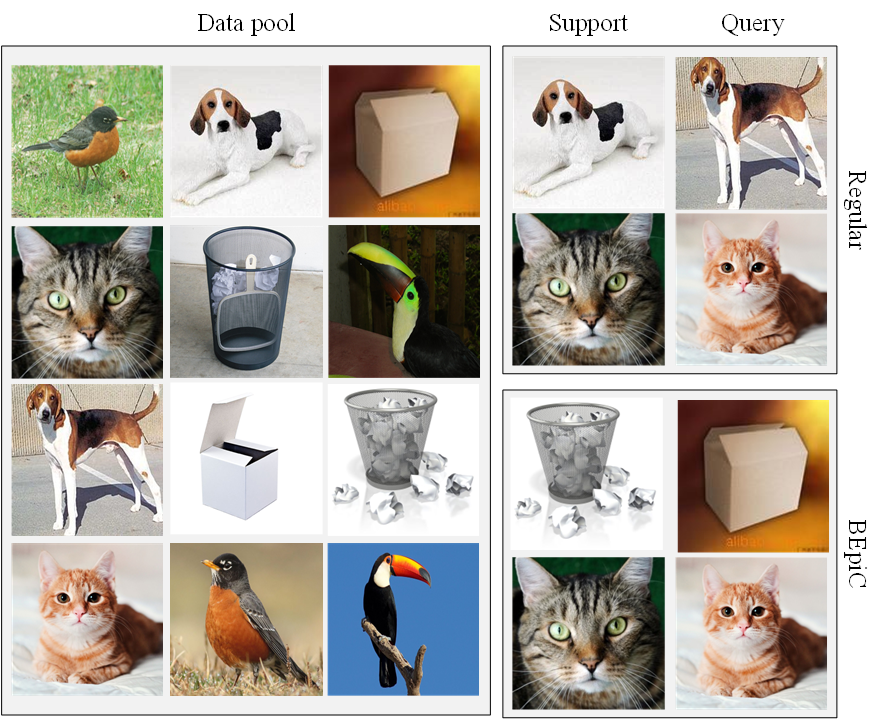
\includegraphics[width=0.9\columnwidth]{FIGURES/bepic/fig.png}
  \caption{Episode generation of Regular and BEpiC from the data pool. In BEpiC, we select the most dissimilar samples.}
  \label{fig:fig}
\end{figure*}

\subsubsection{Samples Selection}

Since the goal of the episode generation is to diversify the samples, sample selection identifies samples that maximize the inter-class distance, which is one of the contributions of our paper. However, computing the distance between every sample across different classes poses a substantial computational challenge, especially for large datasets. To address this, we employ a strategy of randomly designing multiple episodes. For instance, considering a class (referred to as the "cat" class for clarity), we determine which mixture of other classes would yield the most dissimilar set.

The sample selection process involves calculating the centroid of each episode cluster. It is achieved through PCA for dimensionality reduction and mean calculation to determine the centroid. The Euclidean distance metric is then applied to identify the sample closest to the centroid, which is subsequently designated as the class representative. To streamline computations, we later only compare the most centroid images with the ones from the "cat" class. This strategic reduction in the number of comparisons contributes to managing the computational complexity of analyzing large datasets.

We employ the ORB feature-matching algorithm to assess the dissimilarity between samples from the two classes. We select the one with the highest dissimilarity score from a pool of numerous samples. In cases where multiple outputs exhibit the same lowest dissimilarity, we prioritize the first one on the list. This approach ensures we pinpoint the most dissimilar pair of samples, effectively identifying representative class instances. In the following subsection, we provide a brief description of PCA and ORB.

\textbf{PCA:}  Given a dataset \( {X} \in \mathbb{R}^{n \times p} \) with \( n \) observations and \( p \) variables, PCA seeks to find a set of orthogonal vectors, that capture the most variance in the data. The first step in PCA is to subtract the mean of each variable from the dataset \( {X} \), resulting in,

\begin{equation}
{X}_{\text{centered}} = {X} - \bar{{X}}
\end{equation}

Next, we compute the covariance matrix using the center,

\begin{equation}
 {C} = \frac{1}{n-1} {X}_{\text{centered}}^T {X}_{\text{centered}}
\end{equation}

We solve \( {C} {V} = {V} {\Lambda} \) to get eigenvectors \( {V} \) and eigenvalues \( {\Lambda} \) and project the data onto the new coordinate system \( {Y} = {X}_{\text{centered}} {V} \). We select the top \( k \) eigenvectors to reduce the dataset dimensionality: \( {Y}_k = {X}_{\text{centered}} {V}_k \).

The variance explained by the \( i \)-th principal component is \( \frac{\lambda_i}{\sum_{j=1}^p \lambda_j} \), where \( \lambda_i \) is the \( i \)-th eigenvalue.

\textbf{ORB:} ORB calculates the angle intensity based on its center offset, making it suitable for determining orientation., given by
\begin{equation} \label{eq:moment}
\mathrm{m}_{pq}=\sum_{x,y}{x}^{p}{y}^{q}I(x,y)
\end{equation}
where $m$ is referred to as the moment patch, $p$ and $q$ are the sequences of moments comparable to mechanical moments, and $(x, y)$ is the pixel coordinate keypoint of image, $I$. The centroid can then be determined using the moment in \eqref{eq:moment} as
\begin{equation}
C = \left(\frac{m_{10}}{m_{00}},\frac{m_{01}}{m_{00}} \right)
\end{equation}

The centroid will be located using the image's pixel matrix, designated as $\{m_{00}, m_{01}, \cdots\}$. The vector is created by connecting the centroid $C$ with the angle's center. In other words, the patch's orientation can be computed as:

\begin{equation}
\Theta_{orient}=arctan(m_{01},m_{10})
\end{equation}

where $\Theta_{orient}$ is the orientation angle based on the gradients. These selected samples craft the BEpiC episodes using any dataset that contains numerous classes.

\subsection{Dataset}
We conduct experiments on two popular datasets in meta-learning, Caltech 256 \cite{griffin_holub_perona_2022} and miniImageNet \cite{liu2020embarrassingly}. The statistics for the two datasets can be found in Table \ref{table:data}.

\begin{table*}[!ht]
    \centering
    \caption{Statistics from the two image datasets.}
    \begin{adjustbox}{width=0.9\linewidth}
    \renewcommand{\arraystretch}{1.5} 
    \begin{tabular}{|l|l|l|l|l|l|l|}
    \hline
        \textbf{Dataset} & \textbf{\#Classes} & \textbf{\#Training} & \textbf{\#Validation} & \textbf{\#Test} & \textbf{\#Total samples} & 
        \textbf{\#Samples/Class} \\ \hline
        Caltech 256 & 256 & 150 & 56 & 50 & 30,607 & at least 80 \\ \hline
        miniImageNet & 100 & 64 & 16 & 20 & 60,000 & 600 \\ \hline
    \end{tabular}
    \end{adjustbox}
\label{table:data}
\end{table*}

\subsubsection{Caltech 256} The Caltech 256 dataset is considered an enhancement over its predecessor, the Caltech 101 dataset, due to features such as larger category sizes and the inclusion of new and more extensive clutter categories \cite{li_andreeto_ranzato_perona_2022}. This dataset is ideal for developing visual recognition and classification models, comprising 30,607 real-world images across 257 classes of varying sizes (256 object classes plus an additional clutter class). Each class includes 100 training images and 20 test images.

\subsubsection{miniImageNet} miniImagenet, a subset derived from the extensive ImageNet dataset, is specifically tailored for few-shot learning tasks. The unique challenge posed by miniImagenet lies in its demand for machine learning models to generalize effectively with only a limited number of training examples. This dataset consists of 100 classes, each accompanied by 600 images. We allocate 64 classes for training, 16 classes for validation, and 20 classes for testing. This division ensures a balanced distribution of classes across different sets, enabling a comprehensive assessment of model performance.

The experimental evaluation and results are presented in the next sections, which employ the sampling process and dataset.

\subsection{Experimental Evaluation}

We conducted a comprehensive evaluation of our model, focusing on its test accuracy to ensure a thorough examination of its performance. We extended our analysis to encompass the accuracy of various model configurations. The evaluation employed terminologies commonly used in meta-learning research, specifically the $n$-way $k$-shot learning framework, where $n$-way denotes the number of classes and $k$-shot indicates the number of samples the classifier encounters in each training episode. 

For binary classification, the number of ways is fixed as 2-way. However, we vary the $k$-shot classification to explore different configurations with $1, 5, 20$ values. Across all experiments, the total number of epochs is set at $10$, each comprising $10,000$ training episodes and $100$ test episodes.

For every input, the image size is standardized to $(84, 84, 3)$, ensuring uniformity in the dataset preprocessing. This consistent approach to experimental design allows for a thorough investigation of the model's performance under distinct $k$-shot scenarios, shedding light on its adaptability and effectiveness in binary classification tasks.


We experimented with two configurations: 1. exclusively utilizing the BEpiC setup and, 2. incorporating both BEpiC and Regular setups for episode generation. Our findings indicate that the BEpiC configuration exhibits superior generalization compared to the sole use of regular task generation. Moreover, a significant performance enhancement is observed when combining BEpiC with the Regular setup, particularly with increased episodes and shots in each task.

Table \ref{table:bepiC} provides insights into the classifier's performance on the BEpiC test set, where the test class comprises samples from the most dissimilar classes. On the other hand, Table \ref{table:reg+bepiC} outlines the classifier's performance on the BEpiC test set in conjunction with the Regular test data. Lastly, Table \ref{table:random} provides the classifier's performance on random test sets, where both the training and test sets were designed randomly without adhering to our proposed method, implying that the largest inter-class distance was not a focal consideration. These comparative tables underscore the effectiveness and advantages of our proposed approach.

\begin{table}[!ht]
\centering
\caption{Performance of the classifier on the BEpiC test dataset.}
\begin{adjustbox}{width=0.7\linewidth}
\renewcommand{\arraystretch}{1.5} 
\begin{tabular}{|l|l|l|l|l|l|l|}
 \hline
\multirow{3}{*}{\textbf{Train methods}} & \multicolumn{6}{c|}{\textbf{Test accuracy (\%)}}                         \\  \cline{2-7}
                               & \multicolumn{3}{c|}{\textbf{Caltech 256}} & \multicolumn{3}{|c|}{\textbf{miniImageNet}} \\ \cline{2-7}
                               & \textbf{1-shot}  & \textbf{5-shot}  & \textbf{20-shot} & \textbf{1-shot}    & \textbf{5-shot}   & \textbf{20-shot}   \\  \hline
Regular                        & 60.50    & 70.90    & 81.05   & 63.50      & 70.80     & 75.25     \\  \hline
BEpiC                          & \textbf{61.00}      & \textbf{71.90}    & \textbf{81.50}    & \textbf{64.00}        & \textbf{71.00}       & \textbf{76.66}     \\  \hline
Regular+BEpiC                  & \textbf{63.50}    & \textbf{72.80}    & \textbf{81.80}    & \textbf{65.00}        & \textbf{71.40}     & \textbf{76.66}    \\  \hline
\end{tabular}
\end{adjustbox}
\label{table:bepiC}
\end{table}

\begin{table}[!ht]
\centering
\caption{Performance of the classifier on the Regular+BEpiC test dataset.}
\begin{adjustbox}{width=0.7\linewidth}
\renewcommand{\arraystretch}{1.5} 
\begin{tabular}{|l|l|l|l|l|l|l|}
 \hline
\multirow{3}{*}{\textbf{Train methods}} & \multicolumn{6}{c|}{\textbf{Test accuracy (\%)}}                         \\  \cline{2-7}
                               & \multicolumn{3}{c|}{\textbf{Caltech 256}} & \multicolumn{3}{|c|}{\textbf{miniImageNet}} \\ \cline{2-7}
                               & \textbf{1-shot}  & \textbf{5-shot}  & \textbf{20-shot} & \textbf{1-shot}    & \textbf{5-shot}   & \textbf{20-shot}   \\  \hline
Regular                        & 61.00    & 70.00    & \textbf{81.50}   & 65.50  & 69.60     & 76.46     \\  \hline
BEpiC                          & \textbf{62.00}    & \textbf{70.40}  & 80.96  & 65.00    & \textbf{70.50}     & \textbf{76.70}     \\  \hline
Regular+BEpiC                  & \textbf{63.00}    & \textbf{71.97} & 81.25  & \textbf{67.00}    & \textbf{71.00}       & \textbf{76.83}    \\  \hline
\end{tabular}
\end{adjustbox}
\label{table:reg+bepiC}
\end{table}

\begin{table}[!ht]
\centering
\caption{Performance of the classifier on the random test dataset.}
\begin{adjustbox}{width=0.8\linewidth}
\renewcommand{\arraystretch}{1.5} 
\begin{tabular}{|l|l|l|l|l|l|l|}
 \hline
\multirow{3}{*}{\textbf{Train methods}} & \multicolumn{6}{c|}{\textbf{Test accuracy (\%)}}                         \\  \cline{2-7}
                               & \multicolumn{3}{c|}{\textbf{Caltech 256}} & \multicolumn{3}{|c|}{\textbf{miniImageNet}} \\ \cline{2-7}
                               & \textbf{1-shot}  & \textbf{5-shot}  & \textbf{20-shot} & \textbf{1-shot}    & \textbf{5-shot}   & \textbf{20-shot}   \\  \hline
Regular                        & 57.50    & 70.70    & 80.70   & 62.40  &  \textbf{70.20}    &   74.83   \\  \hline
BEpiC (random)                          & \textbf{58.00}    & \textbf{71.00}  & \textbf{81.25}  & \textbf{63.70}    & 70.10     & \textbf{75.33}     \\  \hline
Regular+BEpiC (random)                  & \textbf{61.00}    & \textbf{71.30} & \textbf{81.50}  & \textbf{64.90}    & \textbf{71.16}       & \textbf{76.23}    \\  \hline
\end{tabular}
\end{adjustbox}
\label{table:random}
\end{table}

\subsection{Results and Discussion} \label{results}

The findings from Table \ref{table:bepiC} provide compelling evidence supporting the superiority of BEpiC over Regular episodes in 1-shot classification scenarios. In this context, where test samples encompass any two different categories from the real world, our proposed MAML training method consistently outperforms the conventional approach for both datasets. The subsequent amalgamation of Regular and BEpiC setups results in a noteworthy 2\% and 1.5\% improvement in accuracy for 1-shot classifications on both datasets. This enhancement can be attributed, in part, to the doubled sample size, indicating that the classifier operates more effectively on the intended test samples in this combined arrangement. Expanding the evaluation to 5-shot and 20-shot classifications reveals a consistent trend, with Regular+BEpiC achieving the highest accuracy in all cases for both Caltech 256 and miniImageNet datasets.

The insights from Table \ref{table:reg+bepiC} introduce intriguing nuances to our analysis. In the context of Caltech 256, including Regular test samples alongside BEpiC samples led to a 0.5\% improvement in accuracy for the Regular classifier in 1-shot classification. This improvement is intuitively understandable, as adding Regular test samples facilitated the Regular setup's classification task. Surprisingly, the MAML classifier tested on BEpiC and Regular test samples achieved 1\% higher accuracy than the previous BEpiC-only output. This seemingly counterintuitive result is clarified by recognizing the reduced challenge in classifying Regular test samples due to minimal intra-class distance. Consequently, the classifier excelled in handling Regular samples alongside BEpiC samples, resulting in higher accuracy. Notably, the 20-shot Regular Caltech 256 classification achieved the highest accuracy in this setup, suggesting that Regular test samples favored the Regular approach in achieving higher accuracy in 20-shot scenarios. However, for 5-shot learning, a drop in accuracy across all classifiers indicates the proposed method's increased suitability when there is greater variety in test samples. For miniImageNet, Regular+BEpiC consistently achieved the highest accuracy, except in 1-shot scenarios where BEpiC achieved slightly lower accuracy, with Regular achieving a 0.5\% advantage.

Table \ref{table:random} serves as a cautionary demonstration of the repercussions of disregarding the proposed method. The outputs reveal the necessity of our proposed approach by employing random samples for training episodes, irrespective of their inter-class distance, and testing with a BEpiC setup using random samples. Lower accuracy in 1-shot learning across all outputs compared to Table \ref{table:bepiC} reinforces the importance of strategically selecting samples with higher inter-class distance. This trend persists in 20-shot and 5-shot Caltech 256 scenarios. However, in 5-shot miniImageNet, Regular training outperforms BEpiC (random), affirming the suitability of our proposed method, mainly when training on BEpiC samples with significant intra-class distance.

In summary, the evidence presented consistently advocates for the effectiveness of the proposed BEpiC methodology. Regular+BEpiC emerges as a robust approach, showcasing superior performance across various few-shot learning scenarios compared to conventional and random training methods.

\subsection{Ablation Study}

In our investigation of classifier performance, we systematically varied the number of clusters for the negative class to discern its impact. The choice of cluster count plays a pivotal role in influencing the selection of the most distant samples while considering computational costs. Striking the right balance is crucial for optimizing our research outcomes.

Table \ref{table:5} showcases the classifier's performance with the negative classes drawn from 5 clusters. The results, compared against those from BEpiC in Table \ref{table:bepiC}, are evaluated based on the change in test accuracy (\%). Positive change indicates improved accuracy, while negative values signify a decline. For 5 clusters, there is a consistent drop in test accuracy across all shot learning scenarios, ranging from 0.1\% to 0.66\%. This implies a discernible reduction in classifier performance across various settings when employing 5 clusters.

In Table \ref{table:20}, we extend our analysis to 20 negative class clusters, observing a mixed performance outcome. While some scenarios show improvement, others exhibit marginal decreases. Factors such as multiple clusters being equidistant may contribute to the performance fluctuations. The change in accuracy spans from -0.66\% to 0.27\%. However, the absence of consistent accuracy improvement, coupled with a doubling of computational time, leads us to choose 10 clusters as the optimal value.

Our exploration underscores the delicate trade-off between the number of clusters, computational efficiency, and classifier performance. The choice of 10 clusters emerges as a judicious compromise, balancing enhancing accuracy and managing computational costs in our research endeavors.

\begin{table}[!ht]
\centering
\caption{Performance of the classifier on the random test dataset.}
\begin{adjustbox}{width=0.75\columnwidth}
\renewcommand{\arraystretch}{1.5} 
\begin{tabular}{|l|l|l|l|l|l|l|}
 \hline
\multirow{2}{*}{\textbf{5 Clusters} }  & \multicolumn{6}{c|}{\textbf{Test accuracy (\%)}}                             \\
\cline{2-7}
                            & \multicolumn{3}{c|}{\textbf{Caltech 256}} & \multicolumn{3}{c|}{\textbf{miniImageNet}} \\ \cline{2-7}
                            & \textbf{1-shot}   & \textbf{5-shot}   & \textbf{20-shot}   & \textbf{1-shot}   & \textbf{5-shot}   & \textbf{20-shot}   \\ \hline
BEpiC                     & 60.72    & 71.32    & 81.30      & 63.67     & 70.90     & 76.00        \\ \hline
(\%) change                & -0.28    & -0.58    & -0.20      & -0.33     & -0.10     & -0.66    \\ \hline
\end{tabular}
\end{adjustbox}
\label{table:5}
\end{table}

\begin{table}[!ht]
\centering
\caption{Performance of the classifier on the random test dataset.}
\begin{adjustbox}{width=0.75\columnwidth}
\renewcommand{\arraystretch}{1.5} 
\begin{tabular}{|l|l|l|l|l|l|l|}
 \hline
\multirow{2}{*}{\textbf{20 Clusters} }  & \multicolumn{6}{c|}{\textbf{Test accuracy (\%)}}                             \\
\cline{2-7}
                            & \multicolumn{3}{c|}{\textbf{Caltech 256}} & \multicolumn{3}{c|}{\textbf{miniImageNet}} \\ \cline{2-7}
                            & \textbf{1-shot}   & \textbf{5-shot}   & \textbf{20-shot}   & \textbf{1-shot}   & \textbf{5-shot}   & \textbf{20-shot}   \\ \hline
BEpiC                     & 61.16    & 71.83    & 81.67      & 64.11     & 71.27     & 76.00        \\ \hline
(\%) change               & 0.16    & -0.07    & 0.17      & 0.11    & 0.27     & -0.66    \\ \hline
\end{tabular}
\end{adjustbox}
\label{table:20}
\end{table}

\subsection{Conclusion and Future Work} \label{conclusion}

This study introduces a novel episode generation strategy for binary classification tasks that distinguish between positive and negative classes and comprise various samples. The proposed approach leverages statistical analysis to curate training episodes, emphasizing samples with the highest inter-class distance. The results underscore the proposed method's robustness in effectively identifying test samples using BEpiC episodes. Across all scenarios, the proposed method consistently outperforms classifiers trained through conventional methods, showcasing superior accuracy.

An additional enhancement to the proposed methodology involves the integration of BEpiC with Regular training samples. This hybrid approach adds robustness to the classifiers and improves accuracy. The findings emphasize the potential of combining different training setups to achieve superior performance in binary classification tasks.

This study aims to extend the classifier's capabilities to handle multi-class classification scenarios as part of future work. Additionally, efforts will be directed toward contributing to the evolution of the classifier's architecture to mitigate any overfitting issues. These advancements are expected to broaden the applicability and effectiveness of the proposed meta-learning strategy, fostering its utility in diverse classification tasks.

\section{Task 2: MetaRep: Improving Meta-Learning Accuracy by  Learning Episodic Representation}

\subsection{Introduction}

Traditional machine learning (ML) algorithms require massive datasets to reach their peak performance. In addition, these algorithms also suffer if the test domain slightly deviates from the training domain. Above all, if a new class is introduced, it requires retraining from scratch. On the other hand, human learning is far more advanced as people can learn from only a few samples and distinguish a new class without seeing many examples. This is because humans use their previous experience to learn a new task. Meta-learning, a relatively new branch of  ML,  mimics this process to bridge the gap between ML and human learning with fewer data from different domains  \cite{such2017deep}.

Most meta-learning algorithms \cite{vinyals2016matching,li2017meta,nichol2018reptile,setlur2020support} are centered around the concept of "learning-to-learn," which involves generating tasks or episodes to discern patterns from a limited number of samples. This process entails the training and testing phases, where the samples are partitioned into support and query sets \cite{bennequin2021bridging}. The support set aids in comprehending class representations, while the query set is utilized for inference. To train a meta-learner, batches of data (episodes in meta-learning) are generated by sampling the training data. Therefore, during training, meta-learning algorithms are exposed to a variety of classes that may not be present in the test classes. This allows ample opportunity to incorporate more classes into the training process. However, existing meta-learning approaches fail to fully exploit the potential of abundant training samples to learn episodic representations without label information \cite{hospedales2021meta}. This limitation stems from their reliance on labeled support sets for task adaptation. Moreover, these approaches are primarily designed around supervised learning principles, where labeled samples are necessary for learning \cite{zhang2023learning}. Consequently, the rich diversity in unlabeled data remains unused. To overcome this limitation, a more flexible representation-learning strategy is required that effectively integrates unlabeled data into the episodic learning process to improve model adaptability and performance \cite{tian2020rethinking}.

Representation learning is a widely established way \cite{9770283, 9363924} of boosting classification accuracy in a low-data regime. Typically, representation learning unfolds in two stages  \cite{chen2020simple, grill2020bootstrap}: unsupervised representation learning followed by supervised learning applied to the acquired parameters. However, in the context of meta-learning, where episodes are pivotal, the conventional representation learning approaches designed for batch learning may not be directly implemented in meta-learning. 

To address this challenge, we introduce MetaRep, a representation-learning approach tailored specifically for meta-learning to capture episode-specific representations. MetaRep leverages distinct image augmentation techniques to construct training episodes using unlabeled data. Support sets are formed by randomly sampling from the data pool, and image augmentation techniques are applied to generate query sets. Technically, it works for datasets like Omniglot \cite{lake2015human} and mini-Imagenet \cite{ILSVRC15} or larger datasets because they contain a multitude of samples and classes. Therefore, we hypothesize that the probability of drawing from the same class is insignificant.

MetaRep consists of two steps of training. In the first step, we apply the fully unsupervised training to learn the latent representations of the dataset. Throughout this phase, we utilize the labeled test sets to monitor performance. While the accuracy achieved during unsupervised representation learning may not rival that of supervised learning, the meta-learning algorithm still manages to achieve some degree of accuracy.  Although unsupervised representation falls behind supervised learning accuracy, it is a good initialization point to boost supervised learning performance. Hence, in the second step, we utilize the learned parameters from the unsupervised learning model to initialize the supervised meta-learning process rather than resorting to random initialization. This strategic use of pre-learned parameters effectively transforms the entire process into a semi-supervised meta-learning algorithm \cite{sun2019meta}, thereby enhancing performance.

In addition, MetaRep employs data augmentation to increase learning effectiveness. For an effective augmentation technique, we drew inspiration from SimCLR \cite{chen2020simple} and combined it with color invert and random flip augmentations. This makes the MetaRep model agnostic and adaptable to various meta-learning models. 

To experimentally validate the effectiveness of MetaREP, we evaluated its performance across two prominent meta-learning architectures: Model-Agnostic Meta-Learning (MAML) \cite{finn2017model} and Relation Network (RN) \cite{sung2018learning}. In our experiments, we introduced a modification to the MAML network architecture by integrating temperature \cite{sohn2016improved} into the SoftMax activation function in the inner loop. This adjustment was aimed at mitigating overfitting during unsupervised training. While we retained the RN architecture unchanged, we optimized our hyperparameters and architecture to achieve higher accuracy compared to the results reported in \cite{sung2018learning}. Our experimentation shows that the proposed MetaRep method can enhance the accuracy of any state-of-the-art meta-learning model.

While our approach incorporates techniques like data augmentation and temperature scaling, MetaRep's novelty lies in its unique adaptation for episodic representation learning. Our data augmentation strategy combines methodologies with episodic-specific modifications, creating query samples with demonstrably distinct feature distributions—as verified through our histogram analysis showing entirely new pixel intensities in each run. Unlike previous approaches that produce similar augmented samples, our method introduces meaningful uncertainty between episodes, critical for effective meta-learning where samples may appear across multiple episodes. Complementing this, our introduction of temperature-scaled SoftMax specifically in the meta-learning inner loop addresses the overfitting challenge in unsupervised episodic learning, significantly improving accuracy by forcing the model to learn more discriminative features. Together, these technical innovations enable MetaRep to effectively bridge supervised and unsupervised paradigms by learning transferable episodic representations without labels—representing a fundamental shift from both standard meta-learning approaches that require labeled data for episodic learning and traditional representation learning techniques that aren't optimized for episodic adaptation.

\subsection{Contributions}

Our key contributions are as follows:
\begin{itemize}
    \item We introduce MetaRep, a novel semi-supervised meta-learning framework that leverages unsupervised representation learning to enhance meta-learning performance. Our approach demonstrates significant accuracy improvements across multiple architectures while reducing dependency on labeled data.
    
    \item We develop an enhanced data augmentation strategy that combines SimCLR methodologies with targeted modifications for meta-learning scenarios. Through empirical analysis and visualization, we show how our augmentation technique generates more diverse and informative query sets, leading to improved representation learning.
    
    \item We propose a temperature-scaled adaptation of MAML's inner loop optimization, effectively addressing the overfitting challenges in unsupervised meta-learning. This modification, combined with our optimized implementation of Relation Networks, achieves state-of-the-art performance on standard few-shot learning benchmarks.
    
    \item We validate MetaRep's model-agnostic properties through extensive experimentation across multiple architectures and datasets. Our empirical results demonstrate both cross-architecture adaptability and strong transfer learning capabilities, with MetaRep maintaining consistent performance improvements even when training with significantly reduced labeled data. These results establish MetaRep as a robust, general-purpose enhancement for meta-learning systems.
    
\end{itemize}

\subsection{Related Work}

Meta-learning \cite{hospedales2021meta} has found extensive applications across diverse domains, including self-driving cars, face recognition, and computer vision. While primarily aimed at enabling classification with minimal samples, meta-learning models typically require substantial labeled data for training. This has increased interest in data augmentation techniques within the meta-learning community. Yao et al. \cite{yao2021improving} introduced task augmentation methods, MetaMix and channel shuffle, effectively reducing overfitting by linearly combining features and labels or randomly shuffling channels across classes. Rajendran et al. \cite{rajendran2020meta} proposed a meta-augmentation framework based on information theory to enhance generalization by introducing controlled randomness. However, both approaches remain supervised and still depend significantly on labeled data.

Recent advancements in implicit semantic data augmentation (ISDA) have offered promising alternatives for augmenting training data. Wang et al. \cite{wang2019implicit, wang2021regularizing} proposed ISDA techniques, leveraging semantic transformations within deep feature spaces to efficiently augment datasets and improve model generalization. Their methods implicitly augment data by minimizing upper bounds on the expected loss, significantly enhancing the generalization capabilities of deep networks with minimal computational overhead.

Hsu et al. \cite{hsu2018unsupervised} developed one of the earliest unsupervised meta-learning methods called CACTUs, assigning pseudo-labels through nearest neighbor clustering. Despite its effectiveness, CACTUs is computationally expensive due to additional embedding learning and clustering steps \cite{hartigan1979algorithm}. Moreover, its unsupervised nature limits its accuracy compared to supervised approaches.

Semi-supervised learning has become an active area of research, addressing challenges like limited labeled data and noisy labels. Recent frameworks, such as SimCLR \cite{chen2020simple}, C2MT \cite{zhang2024cross}, and PSSCL \cite{zhang2025psscl}, have proposed advanced strategies for handling limited data and noisy labels. Zhang et al. \cite{zhang2024cross} introduced the cross-to-merge training (C2MT) framework, leveraging cross-training of two networks and balanced data partitioning. PSSCL \cite{zhang2025psscl} focuses on progressively selecting and refining clean data samples, employing contrastive learning for robust semi-supervised training.

To address challenges in domain adaptation and transfer learning scenarios, recent studies have presented innovative approaches. Xie et al. \cite{xie2024adapting} proposed target-oriented transferable semantic augmentation (\text{$T^{2}SA$}), implicitly generating target-like augmented data to enhance model generalization across domains. Their method utilizes class-wise prototype constraints to ensure discriminative and representative augmentation. Additionally, Du et al. \cite{du2024probabilistic} introduced probabilistic contrastive learning (ProCo), effectively addressing issues arising from long-tailed distributions by efficiently sampling contrastive pairs through probabilistic modeling of feature distributions.

Khodadadeh et al. \cite{khodadadeh2019unsupervised} proposed UMTRA, combining unsupervised meta-learning with augmented query samples within the MAML framework. However, its accuracy remains below supervised methods. Chen et al. \cite{chen2020simple} introduced SimCLR, significantly impacting semi-supervised learning through effective data augmentation and a normalized temperature-scaled cross-entropy loss, motivating our approach toward a semi-supervised meta-learning framework integrating representation and transfer learning.

Other prominent meta-learning methods include MAML \cite{finn2017model}, aiming for rapid adaptation through optimized task embeddings. Variants like Reptile \cite{nichol2018reptile}, Meta-SGD \cite{li2017meta}, and LEO \cite{rusu2018meta} have similarly contributed to the field. The Prototypical Network \cite{snell2017prototypical} introduced a metric space for efficient classification, later surpassed by Relation Networks (RN) \cite{sung2018learning}, which further enhanced accuracy. Oreshkin et al. \cite{oreshkin2018tadam} proposed TADAM, enhancing few-shot learning by task-dependent metric scaling and adaptive metrics, significantly improving classification accuracy on benchmark datasets. Lee et al. \cite{lee2019meta} introduced MetaOptNet, utilizing differentiable convex optimization to leverage linear classifiers as base learners, achieving state-of-the-art results in few-shot learning tasks. In our work, we build upon these methods by modifying MAML and leveraging RN, PN, TADAM and MetaOptNet, emphasizing their model-agnostic nature for improved performance.

Additionally, local supervision methods such as InfoPro \cite{wang2024infopro} have emerged, emphasizing information propagation through gradient-isolated modules. InfoPro maximizes useful information retention while efficiently discarding irrelevant features, providing competitive performance with significant computational efficiency, thus complementing existing meta-learning and semi-supervised frameworks.

\begin{figure}[htbp]
    \centering  
    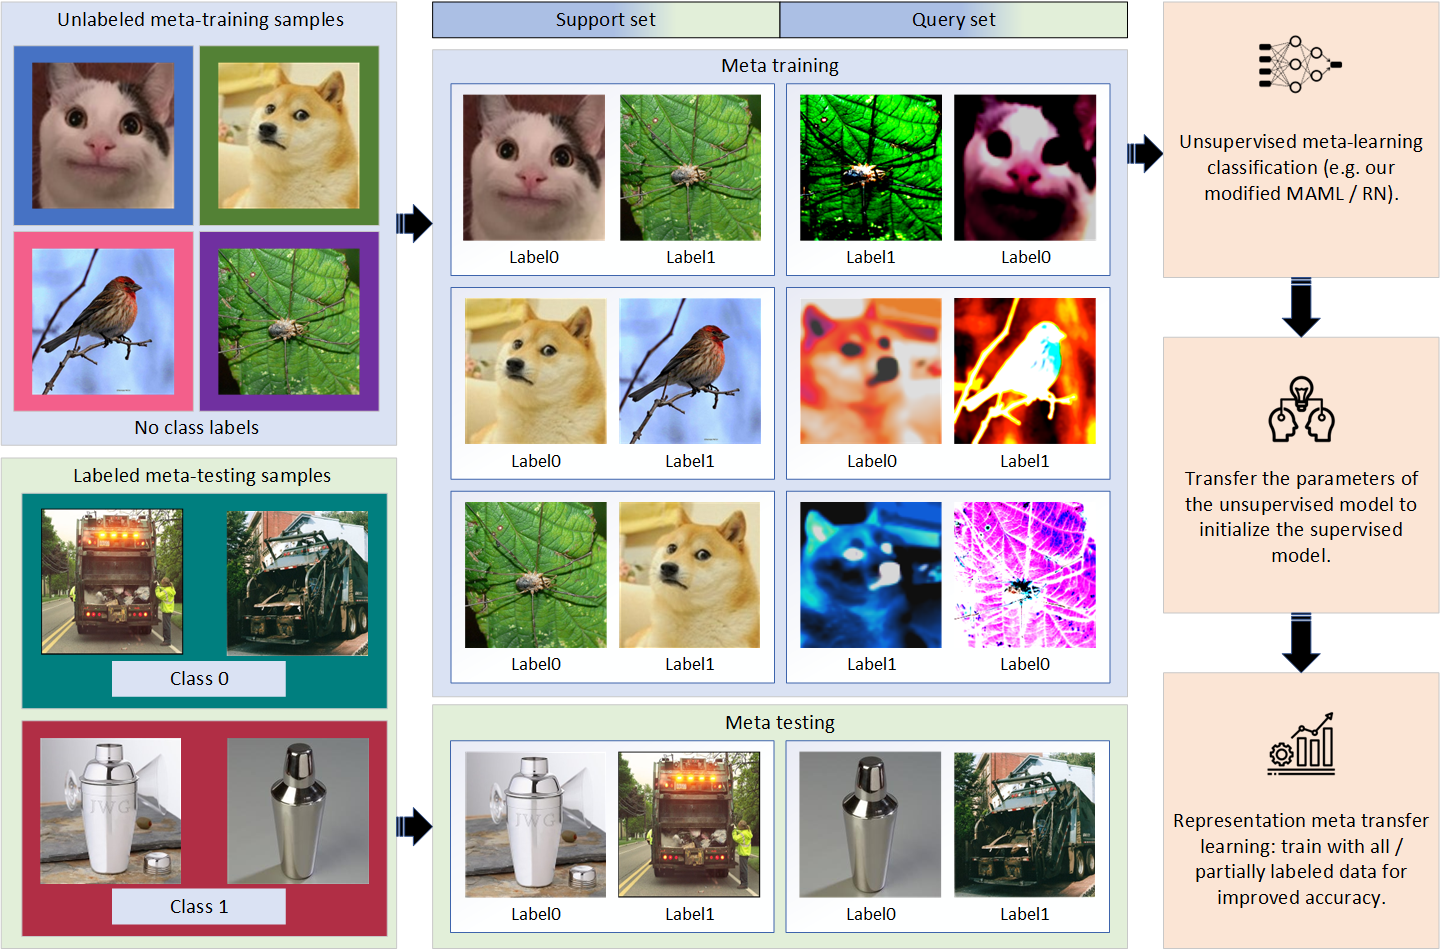
\includegraphics[width=\linewidth]{FIGURES/metarep/corrected.png}
    \caption{Steps of MetaRep, top-left: unlabeled train samples, bottom-left: labeled test samples, middle: episodes for training and testing, middle-left two columns: support set, middle-right two columns: query set, right-top: performing unsupervised meta-learning with the episodes, right-middle: transferring parameters from unsupervised learning to supervised learning, right-bottom: supervised learning with improved accuracy.}
    \label{fig:steps}
  \end{figure}

\subsection{Proposed Method: MetaRep}

In this section, the proposed MetaRep scheme is presented. The MetaRep comprises of two distinct training stages: unsupervised representation learning and semi-supervised meta-learning. A detailed description of each step is presented below. 

\subsubsection{Step 1: Unsupervised Meta-Learning}

\textbf{Data Preparation:} To integrate representation learning with meta-learning, we begin by leveraging either the entire or a subset of the dataset without any label information. Initially, we draw the samples \(x_{n,k}\) from the data pool of \(x_{N}\), where \(n, k\) are the number of ways and the number of shots, respectively, considered in the unsupervised learning and \(N\) is the total number of unlabelled samples. We only design \(n\)-way (or classes), \(1\)-shot support sets because each sample in the support set is drawn randomly, and we cannot randomly add more same-class support samples to that set. However, we can apply data augmentation for the query set to generate multiple query samples of the same class. Subsequently, the effectiveness of generating more query samples is discussed in a later section. 

In episodic learning, every episode sees a combination of new classes. Therefore, after generating the training episodes, assign labeled values \(y_{n,k}\) to each class of the support sets, where \(j\) is the number of ways generated as $\left \{ c_{0},c_{1},...,c_{n-1} \right \}$ and one-hot encoded later. We initialize the random initialization parameter for the unsupervised classifier, $\theta$. We randomly draw the support sets for each task episode and generate the randomly generated support labels. To generate the query set, we pass each sample of the support set through a data augmentation function \(f(A)\) and similarly generate the pseudo labels. Ultimately, we use the regular supervised meta-learning learning test setup to examine the classifier's performance.

\textbf{Deep Dive into Support-Query Set Generation:} We hypothesize that drawing multiple samples from a sizable dataset decreases the likelihood of encountering more than one sample belonging to the same class. Thus, it's imperative to ensure that \(n<<c\) where \(n\) is the number of ways (or the drawn samples, given our 1-shot learning approach) and \(c\) is the total number of classes. However, it is essential to mathematically determine the probability of obtaining unique samples within each class for the datasets used in this study. 

We utilize two distinct datasets: Omniglot and mini-Imagenet. The former typically contains fewer samples per class than the total number of classes, making it highly likely that all drawn samples originate from different classes. Conversely, the mini-Imagenet has more samples (\(600)\) in each class than the total number of classes, resulting in a slightly lower probability of samples originating from different classes. Nonetheless, both datasets feature an equal number of samples per class, denoted as \(m\). Now, we can calculate the probability of the samples belonging to different classes as follows:
\begin{equation}
    P=\frac{c!\cdot m^{n}(c\cdot m-n)}{(c-n)!\cdot (c\cdot m)!}
\end{equation}
\noindent Using the aforementioned formula, the probabilities of 5-way 1-shot classification for the Omniglot (\(1200\) classes) and mini-Imagenet (\(64\) classes) are \(99.21\)\% and \(85.23\)\%, respectively.

Effective data augmentation plays a crucial role in our research, particularly in generating query samples. We combine suggestions from SimCLR \cite{chen2020simple} with additional modifications to enhance effectiveness for RGB image classification, specifically on the mini-Imagenet dataset. The SimCLR paper thoroughly discusses the efficacy of data augmentation and the importance of selecting appropriate augmentation functions, providing valuable insights that guide our approach. They recommend a combination of Gaussian blur, random crop, and random color distortion as the most effective augmentation techniques. Building upon this recommendation, we introduce horizontal flip and random color invert (with a \(50\)\% probability) alongside these three methods. Our experimentation indicates that this augmented combination not only mitigates overfitting but also improves accuracy. Conversely, for the grayscale Omniglot dataset, we solely employ random affine transform. We found that extensive augmentation adversely affects performance, as both support and query samples exhibit significant similarity. Therefore, employing hard augmentation strategies is deemed unnecessary in this particular case.

\textbf{Classifiers:} Our proposed method is model agnostic and can be applied to any model. In this paper, we use two meta-learning models, MAML and RN, to demonstrate the performance on different architectures.  We observe that for MAML, the classifier trained on RGB samples (such as mini-Imagenet in our case) exhibits severe overfitting issues with the regular classifier. This arises because the augmented query samples closely resemble the original support samples, resulting in minimal learning during training. To address this challenge, we introduce a solution by implementing a temperature-scaled SoftMax activation function exclusively within the inner loop of MAML. The inclusion of the temperature term reduces the classifier's confidence in the support set samples, enabling the classifier to gather more information from subtle differences. This adjustment effectively mitigates the overfitting issue, enhancing the performance of MAML. The mathematical expression for temperature-scaled SoftMax is as follows:
\begin{equation}
\frac{\exp(z_{i}/T)}{\sum_{k=0}^{j-1} \exp(z_{k}/T)}
\end{equation}
where the scaling is accomplished by dividing the logits of SoftMax by a value \(T\), known as temperature. \(j\) is the number of ways, and \(z_{i}\), \(z_{k}\) represent the \(i^{th}\), \(k^{th}\) input to the SoftMax, respectively.

We found RN performing counter effectively when using a temperature-scaled SoftMax. We instead used our own set of hyperparameters that led to more improved accuracy than the RN in the original paper.

Following the training of the unsupervised learning algorithm, we preserve the weights and biases for subsequent supervised meta-learning. Consequently, in the classifier of the second step, instead of initializing parameters $\theta$ randomly, we utilize the transferred parameters denoted as $\theta^{*}$. Subsequently, we conduct standard meta-learning procedures to fine-tune and enhance accuracy.

\begin{algorithm}[htbp]
    \caption{MetaRep}
    \label{alg:1}
    \begin{enumerate}
        \item \textbf{Require:} unlabeled dataset $U\{x_N\}$, 
        \item \textbf{Require:} learning rates $\alpha, \beta$, 
        \item \textbf{Require:} augmentation function $f(A)$
        \item Initialize random parameter $\theta$
        \item \textbf{while} not done \textbf{do}
        \begin{enumerate}
            \item Generate episodes $\{x_{n,1}\}$ and create pseudo labels $\{y_{n,1}\}$
            \item \textbf{for each} $(x_{n,1}, y_{n,1})$ \textbf{do}
            \begin{enumerate}
                \item Update the inner loop of meta-learning with custom loss function or hyperparameters
            \end{enumerate}
            \item \textbf{end for}
            \item Update the outer loop of meta-learning with the regular loss function
        \end{enumerate}
        \item \textbf{end while}
        \item Save weights and biases $\theta^*$
        \item \textbf{Input:} Labeled dataset $\{x_{n,k}, y_{n,k}\} \subseteq \{x_{n,1}, y_{n,1}\}$
        \item Initialize $\theta^*$
        \item Perform regular meta-learning steps
    \end{enumerate}
\end{algorithm}

\subsubsection{Step 2: Semi-Supervised Meta-Learning (SSML)}

In this step, we apply SSML within the conventional meta-learning framework, but with parameter initialization from the first classifier. Thus, the transferred parameters originate from the unsupervised meta-learning phase conducted in the initial stage. Let us talk briefly about the two considered classifiers, MAML and RN. Note that we refrain from modifying the SoftMax activation function of MAML at this stage, as the supervised MAML is less prone to overfitting.

\textbf{MAML:} MAML tries to find the optimal parameters $\theta$ derived from a few parametric models $f_{\theta }$. In MAML, we generate the episodes from the data distribution such as $\tau_{i}=(D^{\textrm{tr}},D^{\textrm{val}})$. We use the gradient update to update the initialize parameter $\theta$ to $\theta_{i}^{'}$  across tasks sampled from $p(\tau)$ and is obtained as follows:
\begin{equation}
\theta_{i}^{'}=\theta -\alpha \nabla_{\theta}\pounds_{\tau_{i}}(f_{\theta})
\end{equation}
\noindent where $\alpha$ is the learning rate of the meta-inner loop, and $\pounds$ is the loss function.
In the outer loop of meta-learning, the optimization is performed across tasks via stochastic gradient descent (SGD) to update the $\theta$. It is obtained as follows:
\begin{equation}
\theta\leftarrow \theta -\beta \nabla_{\theta }\sum_{\tau_{i}\sim p(\tau)}\pounds_{\tau_{i}}(f_{\theta^{i}})
\end{equation}
\noindent where $\beta$ is the learning rate of the meta-outer loop.

\textbf{RN:} The main two components of RN are a feature extractor and a relation module. The feature extractor concatenates the features from the support sets, and the query sets as $f_{\varphi}(x_{i})$ and $f_{\varphi}(x_{j})$ through a function $\mathbb{C}(f_{\varphi}(x_{i}),f_{\varphi}(x_{j}))$. 

The combined features are passed through the relation module to obtain their relation score. It is passed through a Sigmoid activation function to obtain the score in a range between 0 to 1. The equation for that is provided below:
\begin{equation}
r_{i,j}=g_{\phi}(\mathbb{C}(f_{\varphi}(x_{i}),f_{\varphi}(x_{j})))
\end{equation}

To create the final output, the relation network's output can also be subjected to extra processing by layers, such as a fully connected neural network. Because of this, the relation network is an adaptable architecture that may be used for various applications. A mean-square-error (MSE) loss function is used to update the network using gradient descent. 
\begin{equation}
\varphi,\phi\leftarrow \arg\min \sum_{i=1}^{m}\sum_{j=1}^{n}(r_{i,j}-1(y_{i}==y_{j}))^{2}
\end{equation}

\textbf{Overall Summary:} The overall method is summarized in this sector with a diagram for better understanding. Figure \ref{fig:steps} depicts the steps of the proposed method. We generate the training episodes from the unlabeled samples. Here, the NT-Xent loss \cite{sohn2016improved} (temperature-scaled SoftMax) is only applied on the MAML for the mini-Imagenet dataset. After training the initial model, we save the parameters and transfer them to the final model for improved performance. Moreover, the pseudo-code for our proposed method is provided in Algorithm \ref{alg:1}.


\textbf{Additional Classifier Architectures:} To comprehensively evaluate MetaRep's model-agnostic capabilities, we implement three additional meta-learning architectures beyond MAML and RN.

\textbf{Prototypical Networks (PN)} \cite{snell2017prototypical} operates by computing class prototypes, the mean feature vector of support samples for each class in an embedding space. Classification is performed by finding the nearest prototype to a query sample using a distance metric (typically Euclidean distance). PN's elegant approach requires no inner loop optimization, making it computationally efficient while maintaining strong performance on few-shot tasks.

\textbf{Task Dependent Adaptive Metric (TADAM)} \cite{oreshkin2018tadam} extends the prototypical network concept by incorporating task conditioning through a Task Embedding Network (TEN). TADAM dynamically adapts its feature extractor for each task using film layers conditioned on task embeddings. Additionally, it employs metric scaling that adjusts the metric space based on task characteristics and leverages auxiliary co-training with standard classification to prevent underfitting. This combination of techniques allows TADAM to achieve superior performance compared to standard meta learning methods.

\textbf{MetaOptNet} \cite{lee2019metaoptnet} frames the inner learning problem as a differentiable convex optimization procedure, specifically using support vector machines (SVMs) for classification. By incorporating this structured classifier rather than a simple linear layer, MetaOptNet leverages the generalization benefits of margin-based classifiers. The SVM's quadratic programming problem is efficiently solved using differentiable optimization techniques, allowing end-to-end training. MetaOptNet is particularly effective in low-data regimes, consistently outperforming other methods on benchmark few-shot classification tasks.

For all three architectures, we apply the MetaRep framework by first learning unsupervised episodic representations, then transferring the learned parameters to initialize supervised meta-learning, following the same procedure as described for MAML and RN.

\subsection{Experiments}

\subsubsection{Data Augmentation for Representation Learning}

We validate our proposed method using two different benchmark datasets in computer vision, Omniglot and mini-Imagenet. Omniglot contains images of handwritten letters from $50$ different languages. This dataset is suitable for few-shot learning because it has $1,623$ characters or classes but only $20$ instances or samples per class. We used $1,200$ classes for training, $100$ classes for validation, and the remaining for testing. In input image dimension to the classifier is $1\times 28\times 28$ pixels, as all are grayscale samples. On the other hand, the mini-Imagenet dataset contains $3\times 84\times 84$ pixels color images. It has a total of $100$ classes, each with $600$ samples. Here, we use $64$ for training, 16 for validation, and $20$ classes for testing.

For selecting the most effective data augmentation, we experimented with different augmentation methods on a trial-and-error basis and found the SimCLR augmentation with an additional augmentation gave the best output for the mini-Imagenet dataset. This section presents the results obtained from various augmentation methods employed in our research. We concentrate on the mini-Imagenet dataset for the augmentation analysis, as the Omniglot dataset typically does not necessitate extensive data augmentation. We also explain why our chosen augmentation works the best for our dataset. Table \ref{tab:unsup} lists the outputs from different augmentation methods using unsupervised learning. Note that all the outputs are obtained by re-implementing different methods using our own hyperparameters, which may provide different results than other literature.

\begin{table}[htbp]
\centering
  \caption{The test accuracy (\%) of unsupervised meta-learning for 5-way 1-shot (5W1S) and 20-way 1-shot (20W1S) classification using mini-Imagenet dataset. For MAML, different temperatures (denoted by ${T}$) are applied in the meta-inner loop.}
 \begin{adjustbox}{width=0.95\linewidth,center}
\tiny
    \begin{tabular}{p{4.5cm}ll|ll}
      \toprule
      \multirow{2}{4.5cm}{\bf Augmentation method} &  \multicolumn{2}{c}{\bf MAML} & \multicolumn{2}{c}{\bf RN} \\
     &  {\bf 5W1S} & {\bf 20W1S} & {\bf 5W1S} & {\bf 20W1S} \\
      \midrule
    \multirow{2}{4.5cm}{Auto augment (UMTRA$^{*}$)}  & 30.1 ($T$=1) & 9.25 ($T$=1) & \multirow{2}{*}{35} & \multirow{2}{*}{9} \\
      & 35.2 ($T$=100) & 11.65 ($T$=10) & &  \\
      \midrule
    \multirow{2}{4.5cm}{Resized crop + Gaussian blur + color distortions (SimCLR)}  & 28.4 ($T$=1)   & 7.6 ($T$=1)   & \multirow{2}{*}{32}   & \multirow{2}{*}{7}  \\
          & 34.4 ($T$=100)    & 11.1 ($T$=10)          &      &   \\
    \midrule
    \multirow{2}{4.5cm}{Horizontal flip (50\%) + color invert (50\%) + resized crop + Gaussian blur + color distortions ({\bf Ours})}    & 33.8 ($T$=1)     & 13.65 ($T$=1)          & \multirow{2}{*}{\bf 39}    &      \multirow{2}{*}{\bf 11.5}     \\
    & {\bf 38.2} ($T$=100)          & {\bf 13.95} ($T$=10)          &          &      \\
      \bottomrule
      $*$re-implementation.
    \end{tabular}
  \end{adjustbox}
  \label{tab:unsup}
\end{table}

\begin{table}[htbp]
  \caption{The test accuracy (\%) of unsupervised meta-learning for 5W1S and 20W1S classification using Omniglot dataset.}
 \begin{adjustbox}{width=\linewidth,center}
\tiny
    \begin{tabular}{p{4.5cm}ll|ll}
      \toprule
      \multirow{2}{4.5cm}{\bf Augmentation method} &  \multicolumn{2}{c}{\bf MAML} & \multicolumn{2}{c}{\bf RN} \\
     &  {\bf 5W1S} & {\bf 20W1S} & {\bf 5W1S} & {\bf 20W1S} \\
      \midrule
    Random transformation + zero pixels (UMTRA$^{*}$) & 48.80 & 24.94 & 61.25 & 35.78 \\
    Resized crop + Gaussian blur (SimCLR) & 48.93 & 27.47 & 66.25 & 43.13  \\
        Random affine transform (30$^{\circ}$) ({\bf MetaRep})  & {\bf 52.83} & {\bf 27.95}  & {\bf 69.12} & {\bf 44.37} \\
      \bottomrule
      $*$re-implementation.
    \end{tabular}
  \end{adjustbox}
  \label{tab:unsup_omni}
\end{table}

From Table \ref{tab:unsup}, we observe the outputs from unsupervised learning for various augmentation functions. Let us begin by discussing the accuracy of MAML. First of all, we use the traditional meta-learning where the temperature parameter in the meta-inner loop for the SoftMax activation function is 1. A temperature of 1 means basically no temperature parameter. For MAML, we discovered that using the optimal temperature in the inner loop increased the accuracy of all the augmentation functions. It is because, when the temperature is 1, the training classifier overfits a lot due to the query set not being very challenging for the support set. When we apply the temperature, the classifier becomes less confident of the classes and can learn more features because of the introduced uncertainty. Initially, we applied the auto-augment function for query sample generation, which achieved slightly higher accuracy than the SimCLR augmentation function in all cases. Our augmentation function achieved 33.8\% and 13.65\% accuracy, which is the highest of all. We introduced temperature parameters as 100 and 10 for 5-way and 20-way, respectively. All the classifiers exhibit improved accuracy for the optimal temperature, and our proposed method obtained the highest accuracy. The temperature is a hyperparameter that shows different performances for different values. In Figure \ref{fig:temp} we illustrated the output accuracy from different temperatures to select the optimal ones. As observed, temperatures 100 and 10 provide the highest accuracy for 5-way and 20-way, respectively.

\begin{figure}[htbp]
    \centering
    \subfloat[\centering 5W1S accuracy for different temperatures.]{{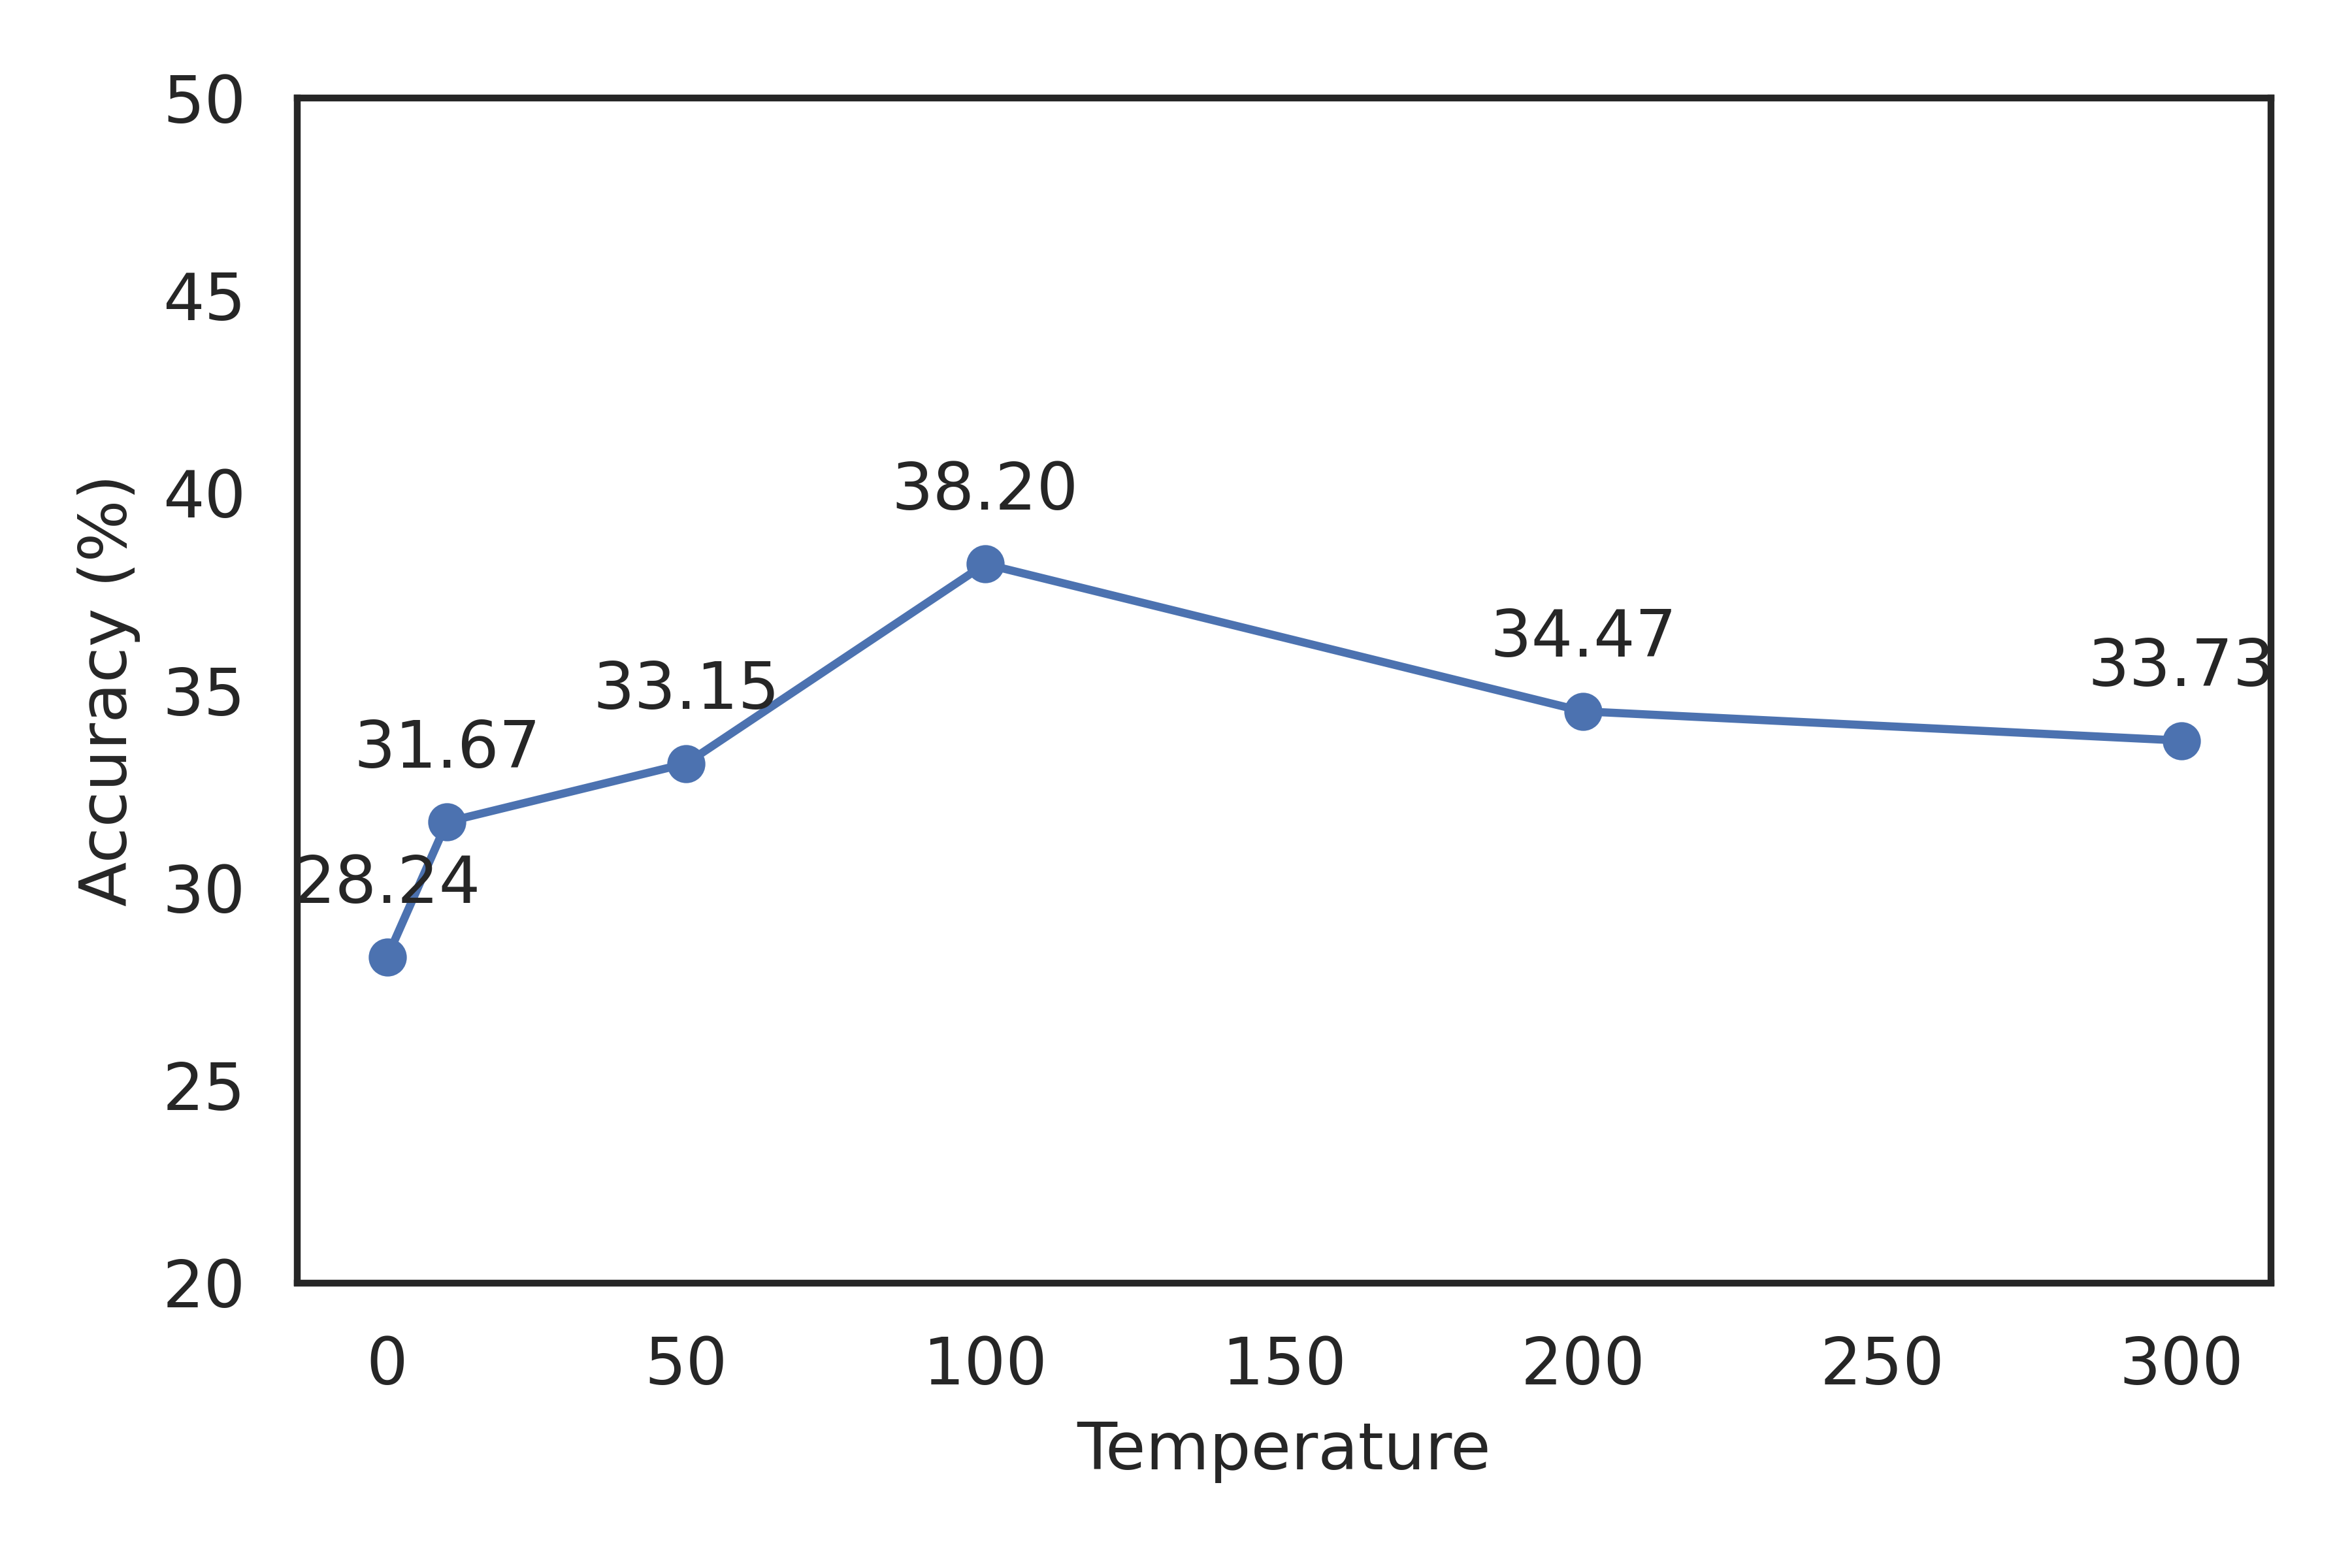
\includegraphics[width=6cm,height=4cm]{FIGURES/metarep/51.png} }}%
    \qquad
    \subfloat[\centering 20W1S accuracy for different temperatures.]{{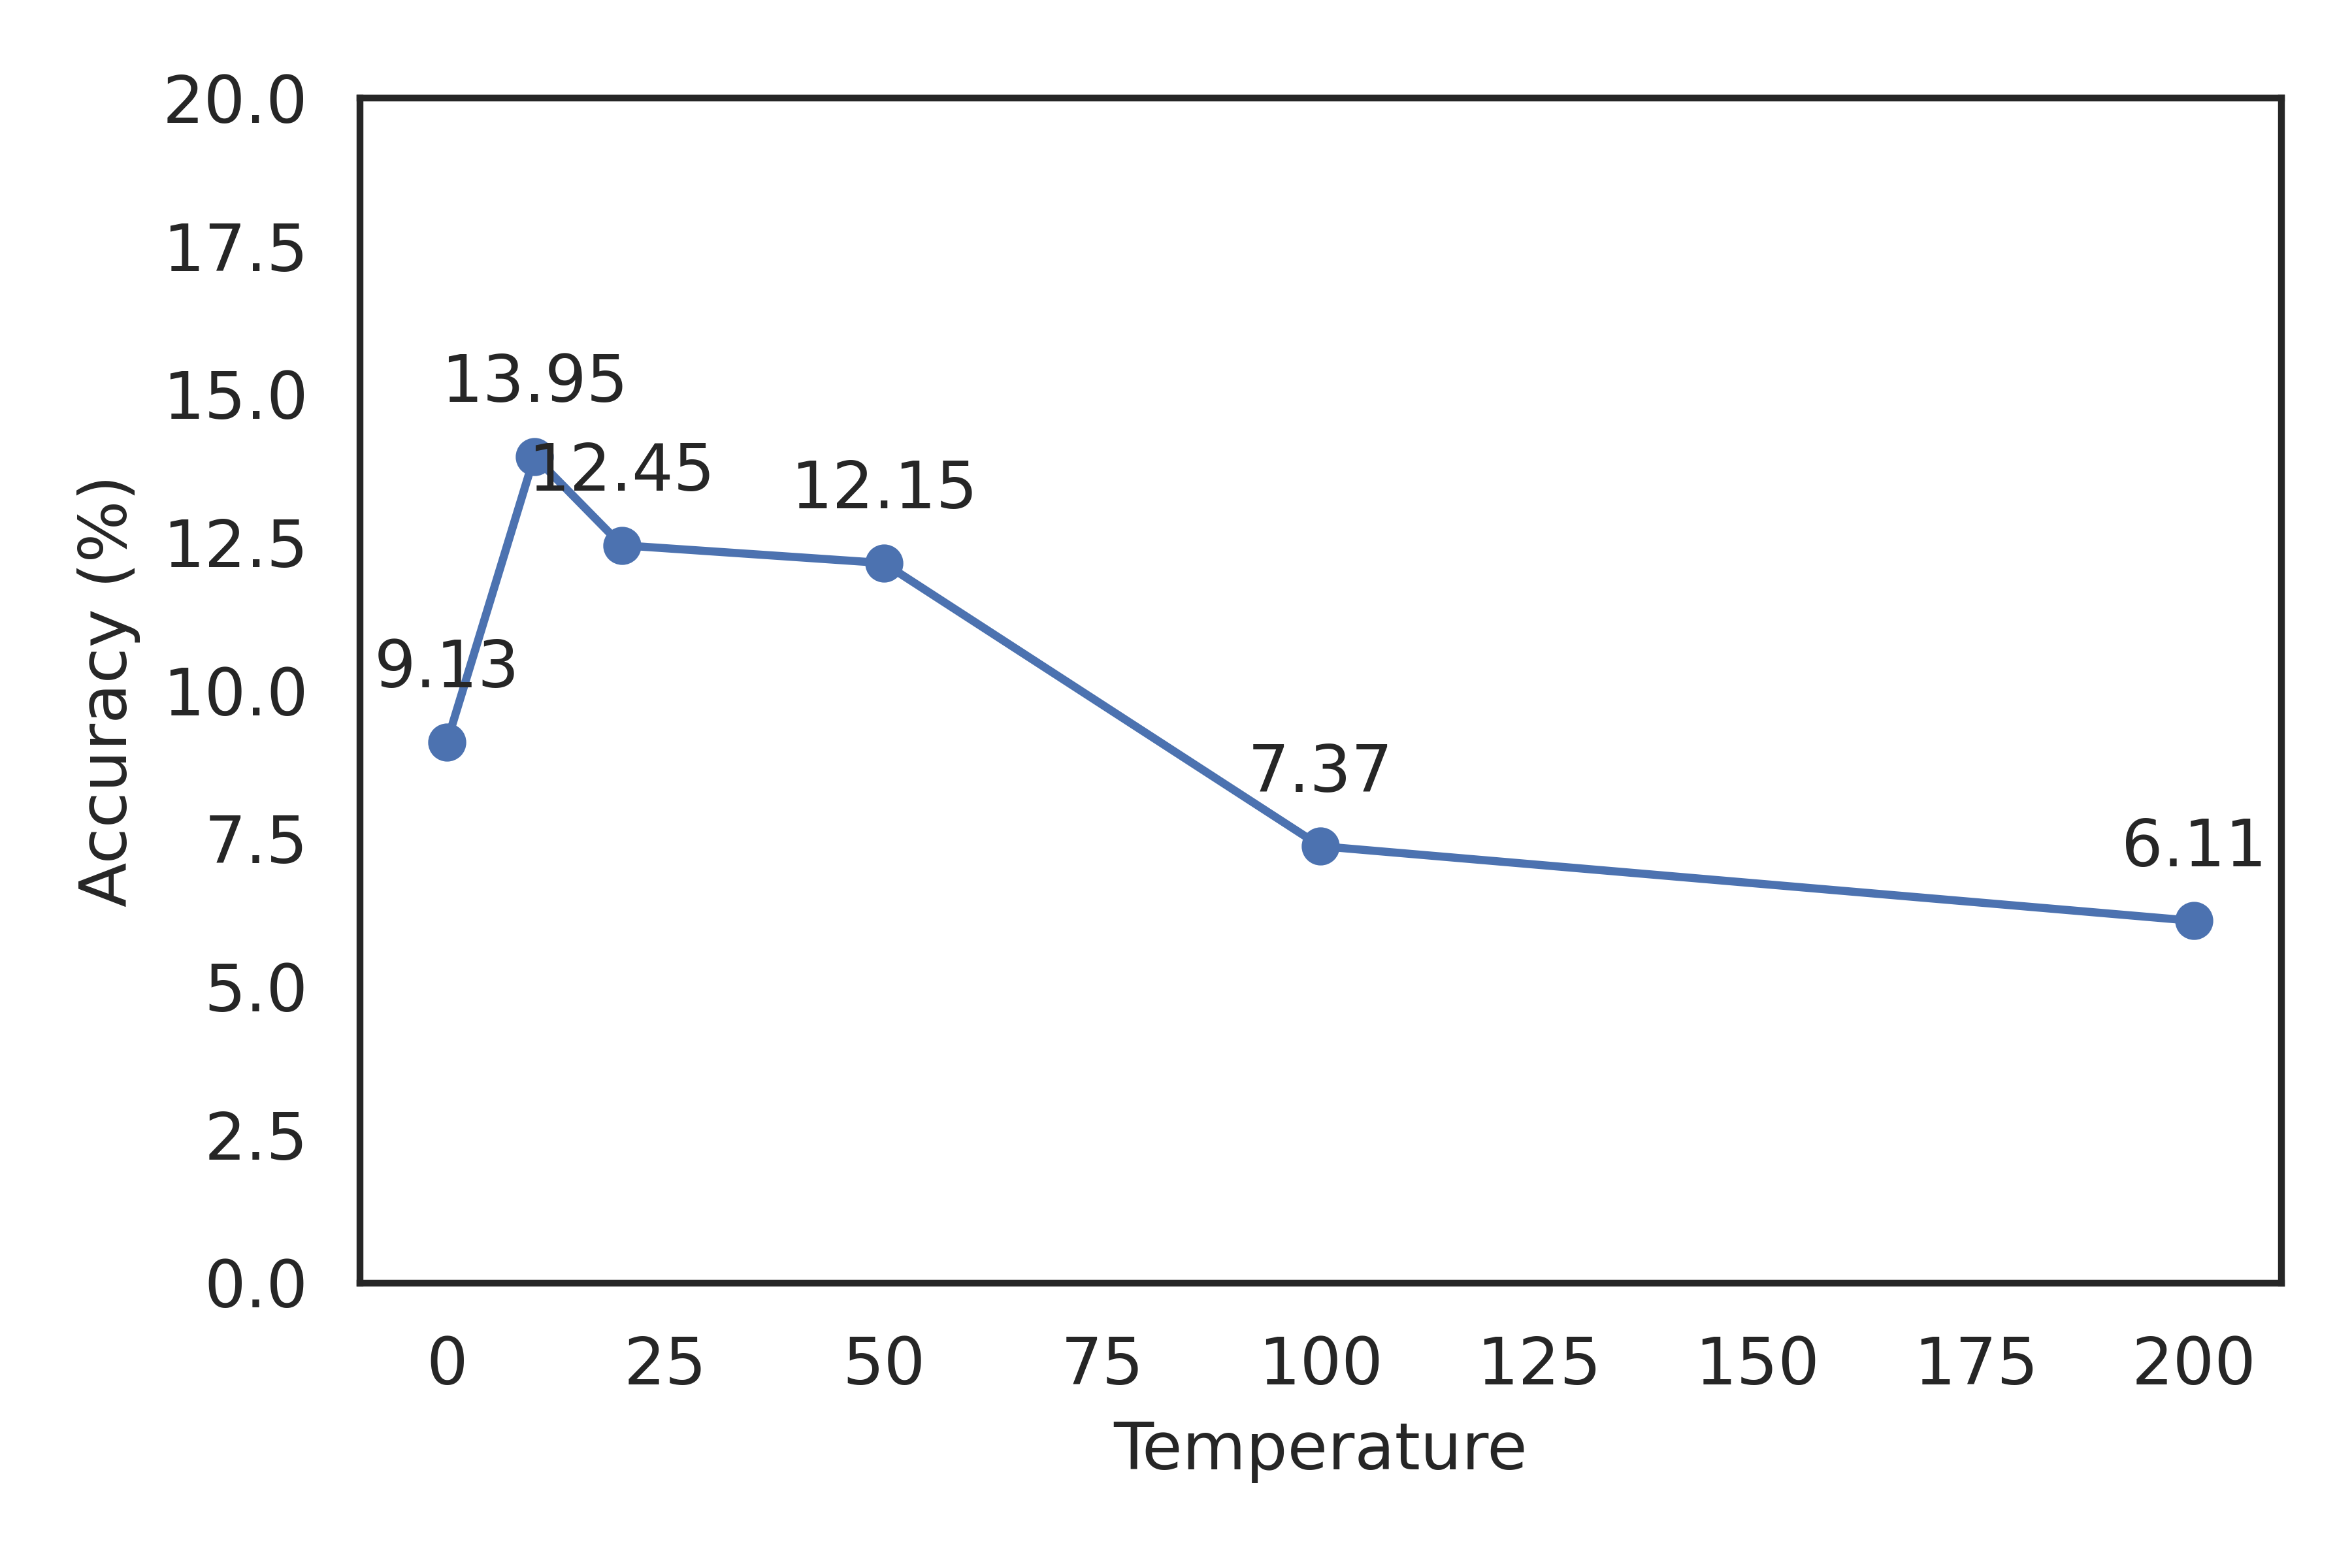
\includegraphics[width=6cm,height=4cm]{FIGURES/metarep/201.png} }}%
    \caption{Effect of different temperatures on test accuracy.}
    \label{fig:temp}
\end{figure}


For the RN, we do not modify anything in the classifier architecture; rather, our motivation is to show that the proposed method is model-agnostic. Nevertheless, our combination of hyperparameters with a ResNet-18 \cite{he2016deep} achieved higher accuracy than MAML for 5-way classification but obtained lower accuracy for 20-way classification. The auto-augment method obtained slightly higher accuracy than the SimCLR augmentation for both 5-way and 20-way classifications. However, SimCLR performs poorly for the 20-way classification and achieves only 7\% accuracy. On the other hand, when we apply our proposed augmentation method, we obtain the highest accuracy for both 5-way and 20-way classifications. Nevertheless, using our proposed method, the RN module achieved higher accuracy than the MAML module for 5-way classification and lower accuracy for 20-way. Therefore, it is evident that the RN unsupervised meta-learning fails to achieve satisfactory accuracy for a higher number of classifications.

We also present the outputs from the Omniglot dataset in Table \ref{tab:unsup_omni} to show the domain adaptability of MetaRep. In Omniglot, the support samples are pretty similar to the query samples. As a result, our experiment found that any hard augmentation on the samples hurt the performance. Therefore, we perform a minimum augmentation to keep the features intact and yet introduce some information in the augmented samples. Moreover, since the samples are grayscale, we could not follow the color distortion function from SimCLR. So, we only applied affine transformation within $30^{\circ}$ to obtain the best transformation. This transformation distorts the samples slightly but keeps the meaning intact. In the case of SimCLR, we only apply resized crop and Gaussian blur as the color distortions do not apply to this dataset. Proof of the effectiveness of our method can be found in the experimental outputs. In this case, the SimCLR augmentation achieved higher accuracy for both MAML and RN in all 5-way 1-shot and 5-way 20-shot classifications. Our proposed method achieves the highest accuracy in all comparisons.

MetaRep can technically be extended to accommodate any n-way 1-shot k-query classification task. This extension is feasible because we have the flexibility to generate different augmented samples in each run for multiple query generation. However, we encountered a drop in accuracy in our proposed model when applied to multiple queries. We attribute this drop in accuracy to the classifier becoming overfit from multiple queries, as they are not distinctly distinguishable. The lack of clear distinctions between multiple query samples likely leads to the classifier being unable to effectively generalize across them, resulting in reduced accuracy. Table \ref{tab:multi-query} represents outputs from MAML for multiple queries. The accuracy drop was significant in all 5-way 5-query and 20-way 5-query shot classifications. Therefore, we do not suggest using our method for a k-query shot. One should instead apply 1-shot unsupervised learning and then transfer the learned parameters to supervised learning. We only applied a 5-way 5-query shot to RN and opted out 20-way 5-query shot because it requires substantial computational resources for a backbone of ResNet-18. In the Omniglot dataset, the accuracy drop for 5-way 5-shot and 20-way 5-shot were 3.68\% and 0.73\% for MAML and 3.87\% and 5.71\% for RN. For mini-Imagenet, the drops are 3.04\% and 1.52\% for MAML and 11\% for RN (N.B. no experiments conducted for 20W1S5Q RN).

\begin{table}[htbp]
  \caption{The test accuracy (\%) and drop of unsupervised MetaRep for n-way, 1-shot multi-query.}
 \begin{adjustbox}{width=\linewidth,center}
\tiny
    \begin{tabular}{p{1.5cm}ll|ll}
      \toprule
      \multirow{2}{1.5cm}{\bf Dataset} &  \multicolumn{2}{c}{\bf MAML} & \multicolumn{2}{c}{\bf RN} \\
     &  {\bf 5W1S5Q} & {\bf 20W1S5Q} & {\bf 5W1S5Q} & {\bf 20W1S5Q} \\
      \midrule
    Omniglot & 49.15 (drop 3.68) & 27.22 (drop 0.73) & 65.25 (drop 3.87) & 38.66 (drop 5.71) \\
    mini-Imagenet & 32.96 (drop 3.04) & 12.43 (drop 1.52) & 28 (drop 11) & N/A \\
      \bottomrule
    \end{tabular}
  \end{adjustbox}
  \label{tab:multi-query}
\end{table}

\begin{figure}[htbp]
  \centering
  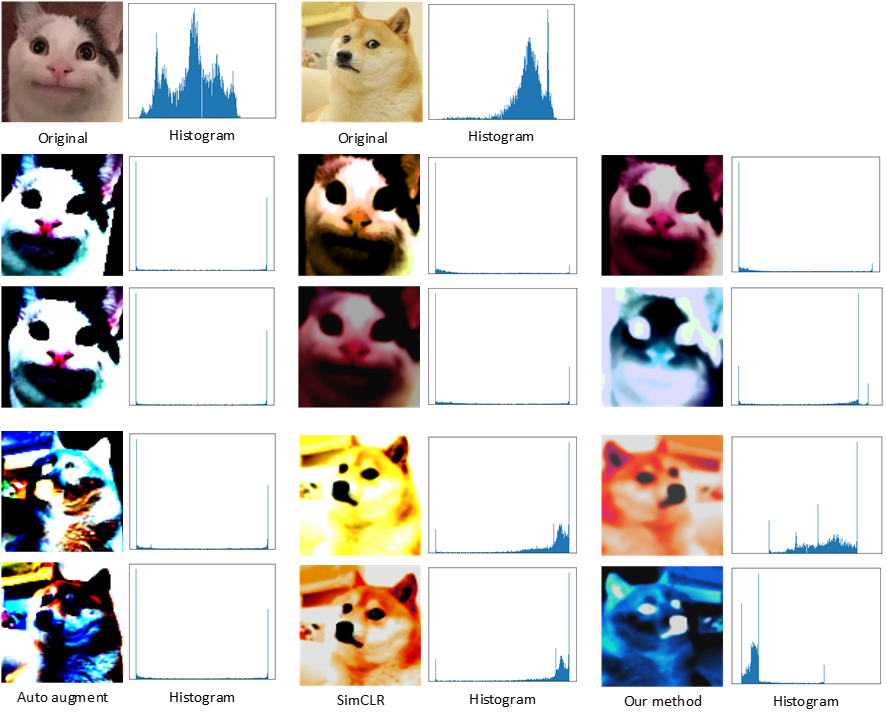
\includegraphics[width=0.8\linewidth]{FIGURES/metarep/figure.png}
  \caption{Histogram of pixel intensities for different augmentation methods.}
  \label{fig:augHist}
\end{figure}

\subsubsection{Computational Resources}

All experiments were conducted using deep learning hardware: a single Nvidia 3080Ti (12GB) GPU for MAML training, and distributed training across two Nvidia 3090Ti (24GB) GPUs plus Google Cloud Platform GPUs for RN, PN, TADAM and MetaOptNet models. Implementation used PyTorch (versions 2.0, 2.3) and Python (versions 3.9, 3.10). For reproducibility, we fixed random seeds to 42, 1234, and 1337 across all experiments.

\subsubsection{Semi-Supervised Meta-Learning (SSML)}

For the second stage, we initialize the meta-learning parameters using weights learned from the unsupervised pre-training phase. To ensure statistical significance, we evaluated all experiments across three random seeds (42, 1234, and 1337). Table \ref{tab:accuracy_omni_mini} presents comprehensive results comparing standard meta-learning approaches with our MetaRep framework across multiple architectures on both Omniglot and mini-ImageNet datasets. All reported accuracies represent means and standard deviations computed across the three independent runs.

Our analysis of Table \ref{tab:accuracy_omni_mini} reveals several important findings across architectures. The baseline model achieves $86.03\pm0.03\%$ on 5W1S1Q for Omniglot, establishing a reasonable lower bound. All meta-learning approaches substantially outperform this baseline, with varying degrees of improvement. 

MetaRep consistently enhances performance across all architectures. For MAML, we observe significant improvements in one-shot learning scenarios (from $93.83\pm0.05\%$ to $96.47\pm0.06\%$ on Omniglot 5W1S1Q), with more modest gains in 5-shot configurations. RN's already strong performance on Omniglot ($99.39\pm0.03\%$ for 5W1S1Q) still improves with MetaRep, reaching perfect $100\%$ accuracy with zero variance. Similarly, PN benefits from MetaRep with accuracy increases from $98.23\pm0.06\%$ to $99.13\pm0.03\%$ on Omniglot 5W1S1Q, and comparable improvements across other configurations.

The advanced architectures TADAM and MetaOptNet also show clear benefits from the MetaRep framework. TADAM's Omniglot performance improves from $99.09\pm0.06\%$ to $100\%$ for 5W1S1Q, while on mini-ImageNet, we observe gains from $57.46\pm0.06\%$ to $58.75\pm0.09\%$. MetaOptNet, despite already achieving optimal performance in several Omniglot configurations, still shows improved consistency in 20W1S1Q (from $98.23\pm0.06\%$ to $99.13\pm0.03\%$) and gains on mini-ImageNet (from $60.36\pm0.09\%$ to $61.23\pm0.06\%$ for 5W1S1Q).

The challenging mini-ImageNet dataset further highlights MetaRep's effectiveness. Across all architectures, we observe consistent improvements: PN ($49.16\pm0.03\%$ to $50.13\pm0.06\%$), MAML ($46.83\pm0.06\%$ to $47.63\pm0.09\%$), RN ($53.03\pm0.06\%$ to $57.03\pm0.09\%$), TADAM ($57.46\pm0.06\%$ to $58.75\pm0.09\%$), and MetaOptNet ($60.36\pm0.09\%$ to $61.23\pm0.06\%$) all benefit from our approach. Particularly noteworthy is RN's substantial 4\% accuracy gain, demonstrating MetaRep's ability to provide more significant benefits to certain architectural paradigms.

The standard deviation values across experiments remain consistently small, indicating the statistical reliability of our results across multiple random seeds. These comprehensive improvements across architectures with different inductive biases strongly validate MetaRep as a truly model-agnostic enhancement to meta-learning frameworks.

\begin{table}[htbp]
  \caption{Classification accuracy (\%) of different methods for random seeds.}
  \centering
  \begin{adjustbox}{width=1.0\linewidth,center}
  \fontsize{9}{9}\selectfont
  \begin{tabular}{p{3cm}cccc|cccc}
  \toprule
  \multirow{2}{*}{\bf Method} & \multicolumn{4}{c|}{\bf Omniglot} & \multicolumn{4}{c}{\bf mini-ImageNet} \\
  & {\bf 1S1Q} & {\bf 5S5Q} & {\bf 20S1Q} & {\bf 20S5Q} & {\bf 1S1Q} & {\bf 5S5Q} & {\bf 20S1Q} & {\bf 20S5Q} \\
  \midrule
  Baseline & $86.03 \pm 0.03$ & $97.67 \pm 0.08$ & $73.03 \pm 0.11$ & $92.37 \pm 0.09$ & $38.47 \pm 0.09$ & $51.23 \pm 0.06$ & N/A & N/A \\
  PN$^{*}$ & $98.23 \pm 0.06$ & $99.13 \pm 0.03$ & $95.63 \pm 0.04$ & $98.53 \pm 0.03$ & $49.16 \pm 0.03$ & $67.86 \pm 0.06$ & N/A & N/A \\
  MAML$^{*}$ & $93.83 \pm 0.05$ & $98.33 \pm 0.06$ & $82.53 \pm 0.06$ & $92.37 \pm 0.06$ & $46.83 \pm 0.06$ & $61.63 \pm 0.03$ & $18.78 \pm 0.09$ & $30.43 \pm 0.06$ \\
  RN$^{*}$ & $99.39 \pm 0.03$ & $100.00 \pm 0.00$ & $97.20 \pm 0.06$ & $99.59 \pm 0.03$ & $53.03 \pm 0.06$ & $64.03 \pm 0.06$ & $24.27 \pm 0.03$ & N/A \\
  TADAM$^{*}$ & $99.09 \pm 0.06$ & $100.00 \pm 0.00$ & $97.57 \pm 0.09$ & $99.69 \pm 0.03$ & $57.46 \pm 0.06$ & $76.27 \pm 0.09$ & N/A & N/A \\
  MetaOptNet$^{*}$ & $100.00 \pm 0.00$ & $100.00 \pm 0.00$ & $98.23 \pm 0.06$ & $100.00 \pm 0.00$ & $60.36 \pm 0.09$ & $76.86 \pm 0.06$ & N/A & N/A \\
  \midrule

  MetaRep PN & $99.13 \pm 0.03$ & $99.73 \pm 0.02$ & $96.23 \pm 0.03$ & $98.77 \pm 0.03$ & $50.13 \pm 0.06$ & $68.41 \pm 0.02$ & N/A & N/A \\
  MetaRep MAML & $96.47 \pm 0.06$ & $98.37 \pm 0.03$ & $83.37 \pm 0.06$ & $92.75 \pm 0.09$ & $47.63 \pm 0.09$ & $61.83 \pm 0.03$ & $18.91 \pm 0.06$ & $30.74 \pm 0.03$ \\
  MetaRep RN & $100.00 \pm 0.00$ & $100.00 \pm 0.00$ & $97.37 \pm 0.06$ & $99.70 \pm 0.03$ & $57.03 \pm 0.09$ & $67.03 \pm 0.06$ & $25.03 \pm 0.06$ & N/A \\
  MetaRep TADAM & $100.00 \pm 0.00$ & $100.00 \pm 0.00$ & $97.90 \pm 0.06$ & $100.00 \pm 0.00$ & $58.75 \pm 0.09$ & $76.94 \pm 0.06$ & N/A & N/A \\
  MetaRep MetaOptNet & $100.00 \pm 0.00$ & $100.00 \pm 0.00$ & $99.13 \pm 0.03$ & $100.00 \pm 0.00$ & $61.23 \pm 0.06$ & $77.11 \pm 0.04$ & N/A & N/A \\
  \bottomrule
  $*$re-implementation.
  \end{tabular}
  \end{adjustbox}
  \label{tab:accuracy_omni_mini}
\end{table}


\begin{table}[htbp]
    \caption{Transferability of MetaRep for different datasets.}
    \begin{adjustbox}{width=0.9\linewidth,center}
    \fontsize{9}{9}\selectfont
    \begin{tabular}{llllll}
    \toprule
    \bf Dataset  & \bf Method    &  \bf 5W1S1Q & \bf 5W5S5Q &  \bf 20W1S1Q & \bf 20W5S5Q \\
    \midrule
    \multirow{6}{*}{CIFAR-FS}       
    & MAML          & $49.63 \pm 0.06$ & $71.23 \pm 0.08$ & $25.79 \pm 0.05$ & $42.19 \pm 0.03$ \\
    & MetaRep MAML  & $53.24 \pm 0.05$ & $71.76 \pm 0.03$ & $26.37 \pm 0.04$ & $42.83 \pm 0.06$ \\
    & RN            & $54.77 \pm 0.04$ & $68.99 \pm 0.05$ & N/A              & N/A              \\
    & MetaRep RN    & $56.08 \pm 0.03$ & $69.70 \pm 0.06$ & N/A              & N/A              \\
    & PN            & $55.36 \pm 0.05$ & $71.67 \pm 0.04$ & N/A              & N/A              \\
    & MetaRep PN    & $57.46 \pm 0.02$ & $73.97 \pm 0.07$ & N/A              & N/A              \\
    \midrule
    \multirow{6}{*}{tieredImageNet} 
    & MAML          & $48.03 \pm 0.04$ & $61.50 \pm 0.05$ & $19.59 \pm 0.06$ & $32.38 \pm 0.03$ \\
    & MetaRep MAML  & $48.23 \pm 0.03$ & $62.07 \pm 0.04$ & $20.13 \pm 0.05$ & $33.26 \pm 0.06$ \\
    & RN            & $51.36 \pm 0.05$ & $67.70 \pm 0.06$ & N/A              & N/A              \\
    & MetaRep RN    & $52.27 \pm 0.04$ & $68.19 \pm 0.03$ & N/A              & N/A              \\
    & PN            & $53.30 \pm 0.06$ & $71.89 \pm 0.05$ & N/A              & N/A              \\
    & MetaRep PN    & $54.68 \pm 0.03$ & $72.07 \pm 0.02$ & N/A              & N/A              \\
    \bottomrule
    \end{tabular}
    \end{adjustbox}
    \label{tab:transfer}
  \end{table}
  
  
\begin{table}[htbp]
    \caption{Accuracy drop (\%) of supervised meta-learning on the partially labeled mini-ImageNet training set.}
    \begin{adjustbox}{width=\linewidth,center}
      \fontsize{9}{9}\selectfont
      \begin{tabular}{p{5cm}llll|llll}
        \toprule
        \multirow{2}{5cm}{\bf Method} 
        & \multicolumn{4}{c|}{\bf 5-way Accuracy} 
        & \multicolumn{4}{c}{\bf 20-way Accuracy} \\
        & {\bf 1S1Q} & {\bf \% Drop} & {\bf 5S5Q} & {\bf \% Drop} 
        & {\bf 1S1Q} & {\bf \% Drop} & {\bf 5S5Q} & {\bf \% Drop} \\
        \midrule
        MAML (50\% labeled data)$^{*}$          & 48.20 & -2.99 & 61.45 & 1.87  & 18.75 & 5.07  & 28.42 & 6.51  \\
        MetaRep MAML (50\% labeled data)        & 49.40 & \textbf{-3.78} & 61.04 & \textbf{1.23}  & 17.94 & \textbf{4.98} & 28.83 & \textbf{6.12} \\
        \midrule
        MAML (25\% labeled data)$^{*}$          & 46.00 & 1.71  & 57.40 & 6.82  & 16.25 & 13.33 & 26.54 & 12.70 \\
        MetaRep MAML (25\% labeled data)        & 47.20 & \textbf{0.84}  & 58.25 & \textbf{5.74}  & 17.50 & \textbf{7.31} & 27.05 & \textbf{11.92} \\
        \midrule
        RN (50\% labeled data)$^{*}$            & 39.00 & 26.42 & 58.20 & \textbf{9.06}   & 19.75 & 18.56 & N/A   & N/A   \\
        MetaRep RN (50\% labeled data)          & 43.00 & \textbf{24.56} & 59.20 & 11.64  & 22.25 & \textbf{11.00} & N/A   & N/A   \\
        \midrule
        RN (25\% labeled data)$^{*}$            & 38.00 & \textbf{28.30} & 51.80 & 19.06  & 18.75 & 22.68 & N/A   & N/A   \\
        MetaRep RN (25\% labeled data)          & 40.00 & 29.82 & 54.40 & \textbf{18.81} & 20.25 & \textbf{19.00} & N/A   & N/A   \\
        \bottomrule
        \multicolumn{9}{l}{$^{*}$Re-implementation results.}
      \end{tabular}
    \end{adjustbox}
    \label{tab:partially_label}
  \end{table}
  
\subsubsection{Computational Complexity Analysis}

We conduct a thorough assessment of MetaRep’s computational overhead relative to standard meta-learning baselines. In particular, MetaRep’s multi-stage training procedure—comprising an unsupervised pre-training step followed by conventional meta-training—incurs additional resource demands. Table \ref{tab:computational_requirements} presents the training time and memory requirements for different model configurations.

MetaRep introduces approximately 30\% to 60\% additional computational time during training due to the unsupervised pre-training phase. However, this overhead occurs only during the initial model development and does not affect inference time, which remains identical to the base models. The enhanced accuracy (3-4\% improvement) and reduced labeled data requirements (up to 75\% reduction) justify this one-time computational cost for most applications.

\begin{table}[htbp]
  \centering
  \caption{Computational Requirements Comparison for 5‐way 5‐shot classification.}
  \label{tab:computational_requirements}
  \begin{adjustbox}{width=\linewidth,center}
  \begin{tabular}{lcccc}
      \toprule
      \textbf{Method} & \textbf{Trainable Parameters} & \textbf{GPU Memory (GB)} & \textbf{Training Time (hours)} & \textbf{Inference Time (ms/episode)} \\
      \midrule
      MAML         &  32.9K & 1.4  & 2 & 12 \\
      MetaRep MAML &  32.9K  & 1.4 & 3.5 & 12 \\
      RN           &  8.54M  &  4.8  & 12 & 30 \\
      MetaRep RN   &  8.54M  & 4.8 & 19 & 30 \\
      TADAM        &   8.0M & 4.2 &  8 &  48 \\
      MetaRep TADAM    & 8.0M & 4.2 &  14.5 &  48 \\
      MetaOptNet   &  12M &  8.3 &  14 &  60 \\
      MetaRep MetaOptNet & 12M & 8.3 &  25 &  60 \\
      \bottomrule
  \end{tabular}
\end{adjustbox}
\end{table}

\subsubsection{Transferability of MetaRep}

To evaluate the cross-dataset generalization capabilities of MetaRep, we conducted transfer learning experiments using CIFAR-FS \cite{DBLP:journals/corr/abs-1805-08136} and tieredImageNet \cite{DBLP:journals/corr/abs-1803-00676} datasets. For these experiments, we transferred representations learned from the mini-ImageNet dataset. To ensure statistical significance, all experiments were evaluated across three random seeds (42, 1234, and 1337). All reported accuracies represent means and standard deviations computed across the three independent runs. CIFAR-FS contains 100 classes with 600 images per class, split into 64 classes for training, 16 for validation, and 20 for testing. The larger tieredImageNet dataset comprises 608 classes and 779,165 total images, with 351 classes allocated for training, 97 for validation, and 160 for testing.

Table~\ref{tab:transfer} presents comprehensive results across multiple architectures (MAML, RN, and PN) and evaluation scenarios. For each configuration, we report mean accuracies with standard deviations across three random seeds. The results demonstrate consistent improvements when applying MetaRep across all architectures and datasets.

On \textbf{CIFAR-FS}, we observe particularly substantial improvements for 5-way 1-shot classification: MAML ($49.63 \pm 0.06\%$ to $53.24 \pm 0.05\%$, a $3.61\%$ increase), RN ($54.77 \pm 0.04\%$ to $56.08 \pm 0.03\%$, a $1.31\%$ increase), and PN ($55.36 \pm 0.05\%$ to $57.46 \pm 0.02\%$, a $2.10\%$ increase). The improvements remain consistent but more modest for 5-way 5-shot classifications.

For \textbf{tieredImageNet}, while the absolute performance improvements are smaller, MetaRep still provides consistent gains across all architectures. The Prototypical Network exhibits the largest improvement for 5-way 1-shot classification (from $53.30 \pm 0.06\%$ to $54.68 \pm 0.03\%$), while MAML shows the most substantial relative improvement in the 20-way scenarios (e.g., from $19.59 \pm 0.06\%$ to $20.13 \pm 0.05\%$ for 20-way 1-shot). The consistent improvements across diverse datasets demonstrate that MetaRep learns transferable representations that generalize beyond the source domain.

\subsection{Why Our Method is Effective}

In Figure \ref{fig:augHist}, we explained why MetaRep works effectively by visualizing the pixel intensities from the histograms of augmented images. This histogram analysis illustrates the degree of uncertainty introduced in different augmented samples compared to the original samples. We observe that in both auto-augment and SimCLR augmentation, the histograms of augmented samples exhibit striking similarity to each other. This indicates that all augmented samples fail to introduce sufficient new uncertainties in each augmentation. This aspect is crucial because a sample can frequently appear in meta-learning across different episodes. Hence, we must supply query samples with distinguishable features in each run. 

On the other hand, our proposed augmentation method demonstrates histograms with entirely new pixel intensities for each run. This implies that the features contain new information in each query sample. This observation can be attributed to the uncertainty introduced in our augmentation function through the horizontal flip and color invert operations, each with a 50\% probability. As a result, our proposed method achieves the highest accuracy for unsupervised meta-learning.

\subsection{Ablation Study}

Additionally, we highlight that MetaRep can obtain high accuracy or less accuracy loss for partially labeled datasets (Table \ref{tab:partially_label}). We specifically conduct this analysis on the mini-Imagenet dataset due to its larger class size (600 samples per class), whereas Omniglot only contains 20 samples per class. We randomly select 50\% (300) and 25\% (150) training samples from the mini-Imagenet data and train our classifier to compare the proposed and original methods. This time we report the percentage accuracy drop from the main output (trained on 100\% samples) to have a fair comparison between the original method and MetaRep. It is obtained as $((All \: Labeled \: Accuracy - Partially \: Labeled \: Accuracy) / All \: Labeled \: Accuracy)\times 100\%$. In most outputs, our proposed method has less drop except for MetaRep RN with 50\% and 25\% labeled data for 5W5S5Q and 5W1S1Q, respectively. 

Notably, in MAML and MetaRep MAML for 5W1S1Q, we observe negative accuracy drop percentages. This unexpected result occurs because the accuracy actually increases when we train MAML with 50\% data in this setup. We hypothesize that this improvement stems from episode generation with fewer samples in each class. Some research suggests that having a large number of meta-training data can counterintuitively degrade performance due to the lower probability of all samples appearing in episodes. For example, Triantafillou et al.  \cite{triantafillou2019meta} found that having a large meta-dataset hurts the accuracy of the mini-Imagenet dataset. Setlur et al. \cite{setlur2020support} showed that having a fixed support set and having less diversity can improve accuracy. This emerging research direction focuses on determining the optimal number of samples in meta-training and devising more effective episode-generation strategies. We aim to focus on this area in our future research.

\subsection{Future Work}

While MetaRep demonstrates strong performance on standard few-shot learning benchmarks, real-world applications such as medical image diagnosis and autonomous driving involve additional challenges. For example, medical diagnosis demands high interpretability, robustness to noise, and strict regulatory standards, whereas autonomous driving requires real-time inference under dynamic conditions and sensor fusion from multiple modalities. MetaRep's reliance on episodic training and data augmentation may need further adaptation to address these domain-specific requirements. In particular, augmentation strategies effective for natural images (e.g., in mini-ImageNet) may not translate well to medical imaging due to the clinical significance of subtle features. Furthermore, the episodic structure might not directly map to the continuous and streaming data in autonomous systems. Addressing these concerns could involve incorporating domain-specific priors into the augmentation pipeline, improving robustness under distribution shifts, or integrating MetaRep with multi-modal representation learning.

Our experiments revealed interesting dynamics regarding temperature sensitivity across different task configurations. Future work should explore more sophisticated confidence calibration mechanisms that adapt dynamically to task complexity. Promising approaches include dynamic temperature scaling based on feature-to-cluster center distances, adaptive confidence penalties, task-conditional calibration, or meta-learned calibration parameters. These methods could potentially enhance MetaRep's adaptability across varying task complexities without requiring manual hyperparameter tuning.

Additionally, exploring the relationship between episodic diversity and model performance represents another important research direction. Our findings with partially labeled datasets suggest that carefully curated episodes might outperform those generated from larger but potentially redundant data pools. Developing systematic approaches to episode generation and support set construction could further improve meta-learning efficiency and effectiveness, particularly in resource-constrained scenarios. We consider these directions important avenues for future work to ensure MetaRep's effectiveness in safety-critical and high-impact real-world scenarios.

\subsection{Conclusion}

In this research, we propose MetaRep, a novel strategy that utilizes unsupervised meta-learning to derive latent representations from datasets, which are then employed for SSML with the learned parameters. This approach significantly enhances the performance of supervised learning, making our method both rapidly adaptive and highly accurate. Effective data augmentation for query sample generation is a cornerstone of our unsupervised approach, and we visually demonstrate the superiority of our augmentation strategies over others. Additionally, temperature-scaled SoftMax plays a crucial role in improving unsupervised classification accuracy. Tested on two different datasets and models, MetaRep consistently achieves better test accuracy compared to original methods and maintains strong performance with partially labeled training samples, showcasing its efficiency and robustness across various scenarios.

\section{Task 3: Meta-Task: A Method-Agnostic Framework for Learning to Regularize in Few-Shot Learning}

\subsection{Introduction}

Few-Shot Learning (FSL) has emerged as a promising solution to the problem of data scarcity in machine learning, particularly in computer vision, medical applications, and personalized health systems \cite{nayem2023few, PFM_Ali, Event_Ali}. By leveraging meta-learning, FSL enables models to learn how to learn with the primary objective of extracting meaningful, transferable representations from sparse datasets, reducing the need for extensive labeled data, and significantly lowering data collection and annotation costs \cite{metasgd,zhang2018metagan}.

Advances in meta-learning have led to techniques such as Matching Networks~\cite{NIPS2016_90e13578}, Relation Networks~\cite{sung2018learning}, Model-Agnostic Meta-Learning (MAML) \cite{maml}, Prototypical Networks \cite{snell2017prototypical}, and Reptile~\cite{nichol2018reptile}. Despite performance gains, FSL models remain prone to overfitting, limiting generalization.

Regularization plays a critical role in mitigating overfitting and enhancing generalization in FSL. Conventional methods such as weight decay\cite{krogh1991simple}, dropout\cite{hinton2012improving}, and noise injection\cite{achille2018information, tishby2015deep} fail to address FSL-specific challenges. Meta-learning requires both adaptation-generalization and meta-generalization\cite{rajeswaran2019imaml, mrmaml, pan2021meta, wang2023improving, yao2021meta, yao2021improving, rajendran2020meta}, yet existing techniques remain static, inflexible, and reliant on manually designed loss functions or auxiliary tasks that do not adapt to the unique structure of each task. This limitation motivates the need for a more dynamic, learnable regularization mechanism.

To address this limitation, we introduce Meta-Task, a method-agnostic framework that reformulates regularization as a learnable task within the FSL optimization process. Meta-Task dynamically learns task-specific regularization strategies through a parameterized neural layer $\phi$. This adaptive mechanism enables our framework to seamlessly integrate with existing FSL pipelines, ensuring flexibility across different task distributions and learning paradigms. Meta-Task remains compatible with existing auxiliary tasks and regularization losses, leveraging prior techniques while introducing a dynamic, learnable component. This enhances overfitting mitigation without extensive hyperparameter tuning or task-specific modifications, making it scalable and practical for real-world FSL applications.

To operationalize Meta-Task regularization, we propose using an autoencoder-based Task-Decoder (Figure \ref{fig:1}). The Task-Decoder serves as a flexible and effective regularizer, refining task-specific representations by constraining the embedding vector to reconstruct the original input accurately. We choose autoencoders because they are data-agnostic, easy to implement, architecturally flexible, and allow tunable parameterization for optimization. This adaptability makes them well-suited for various FSL applications, as they can seamlessly integrate into different model architectures.

Our method leverages the latent variable $z$, inherently present in most FSL settings due to the N-Way, K-Shot paradigm. The standard inner-outer loop optimization structure ensures the existence of an intermediate latent representation within the support-query split or gradient-based adaptation process. This guarantees compatibility across various FSL architectures, allowing Meta-Task to enhance regularization effectiveness dynamically.

\subsection{Contributions}

Our main contributions are:
\begin{enumerate}
    \item \textbf{Meta-Task Framework:} We propose Meta-Task, a novel, method-agnostic framework that introduces auxiliary tasks to regularize individual tasks in FSL.
    
    \item \textbf{Task-Decoder (Figure \ref{fig:1}):} We introduce the Task-Decoder, utilizing autoencoders as a new regularization task for meta-learners, leveraging unsupervised learning to refine hidden representations.
    
    \item \textbf{Improved Performance:} Our method demonstrates faster convergence, higher accuracy, and better generalization than existing techniques, all without extensive hyperparameter tuning.
    
    \item \textbf{Versatility and Applicability:} The framework is method-agnostic and can be integrated with various FSL settings, making it suitable for real-world, resource-constrained scenarios.
\end{enumerate}

\begin{figure}
  \centering
   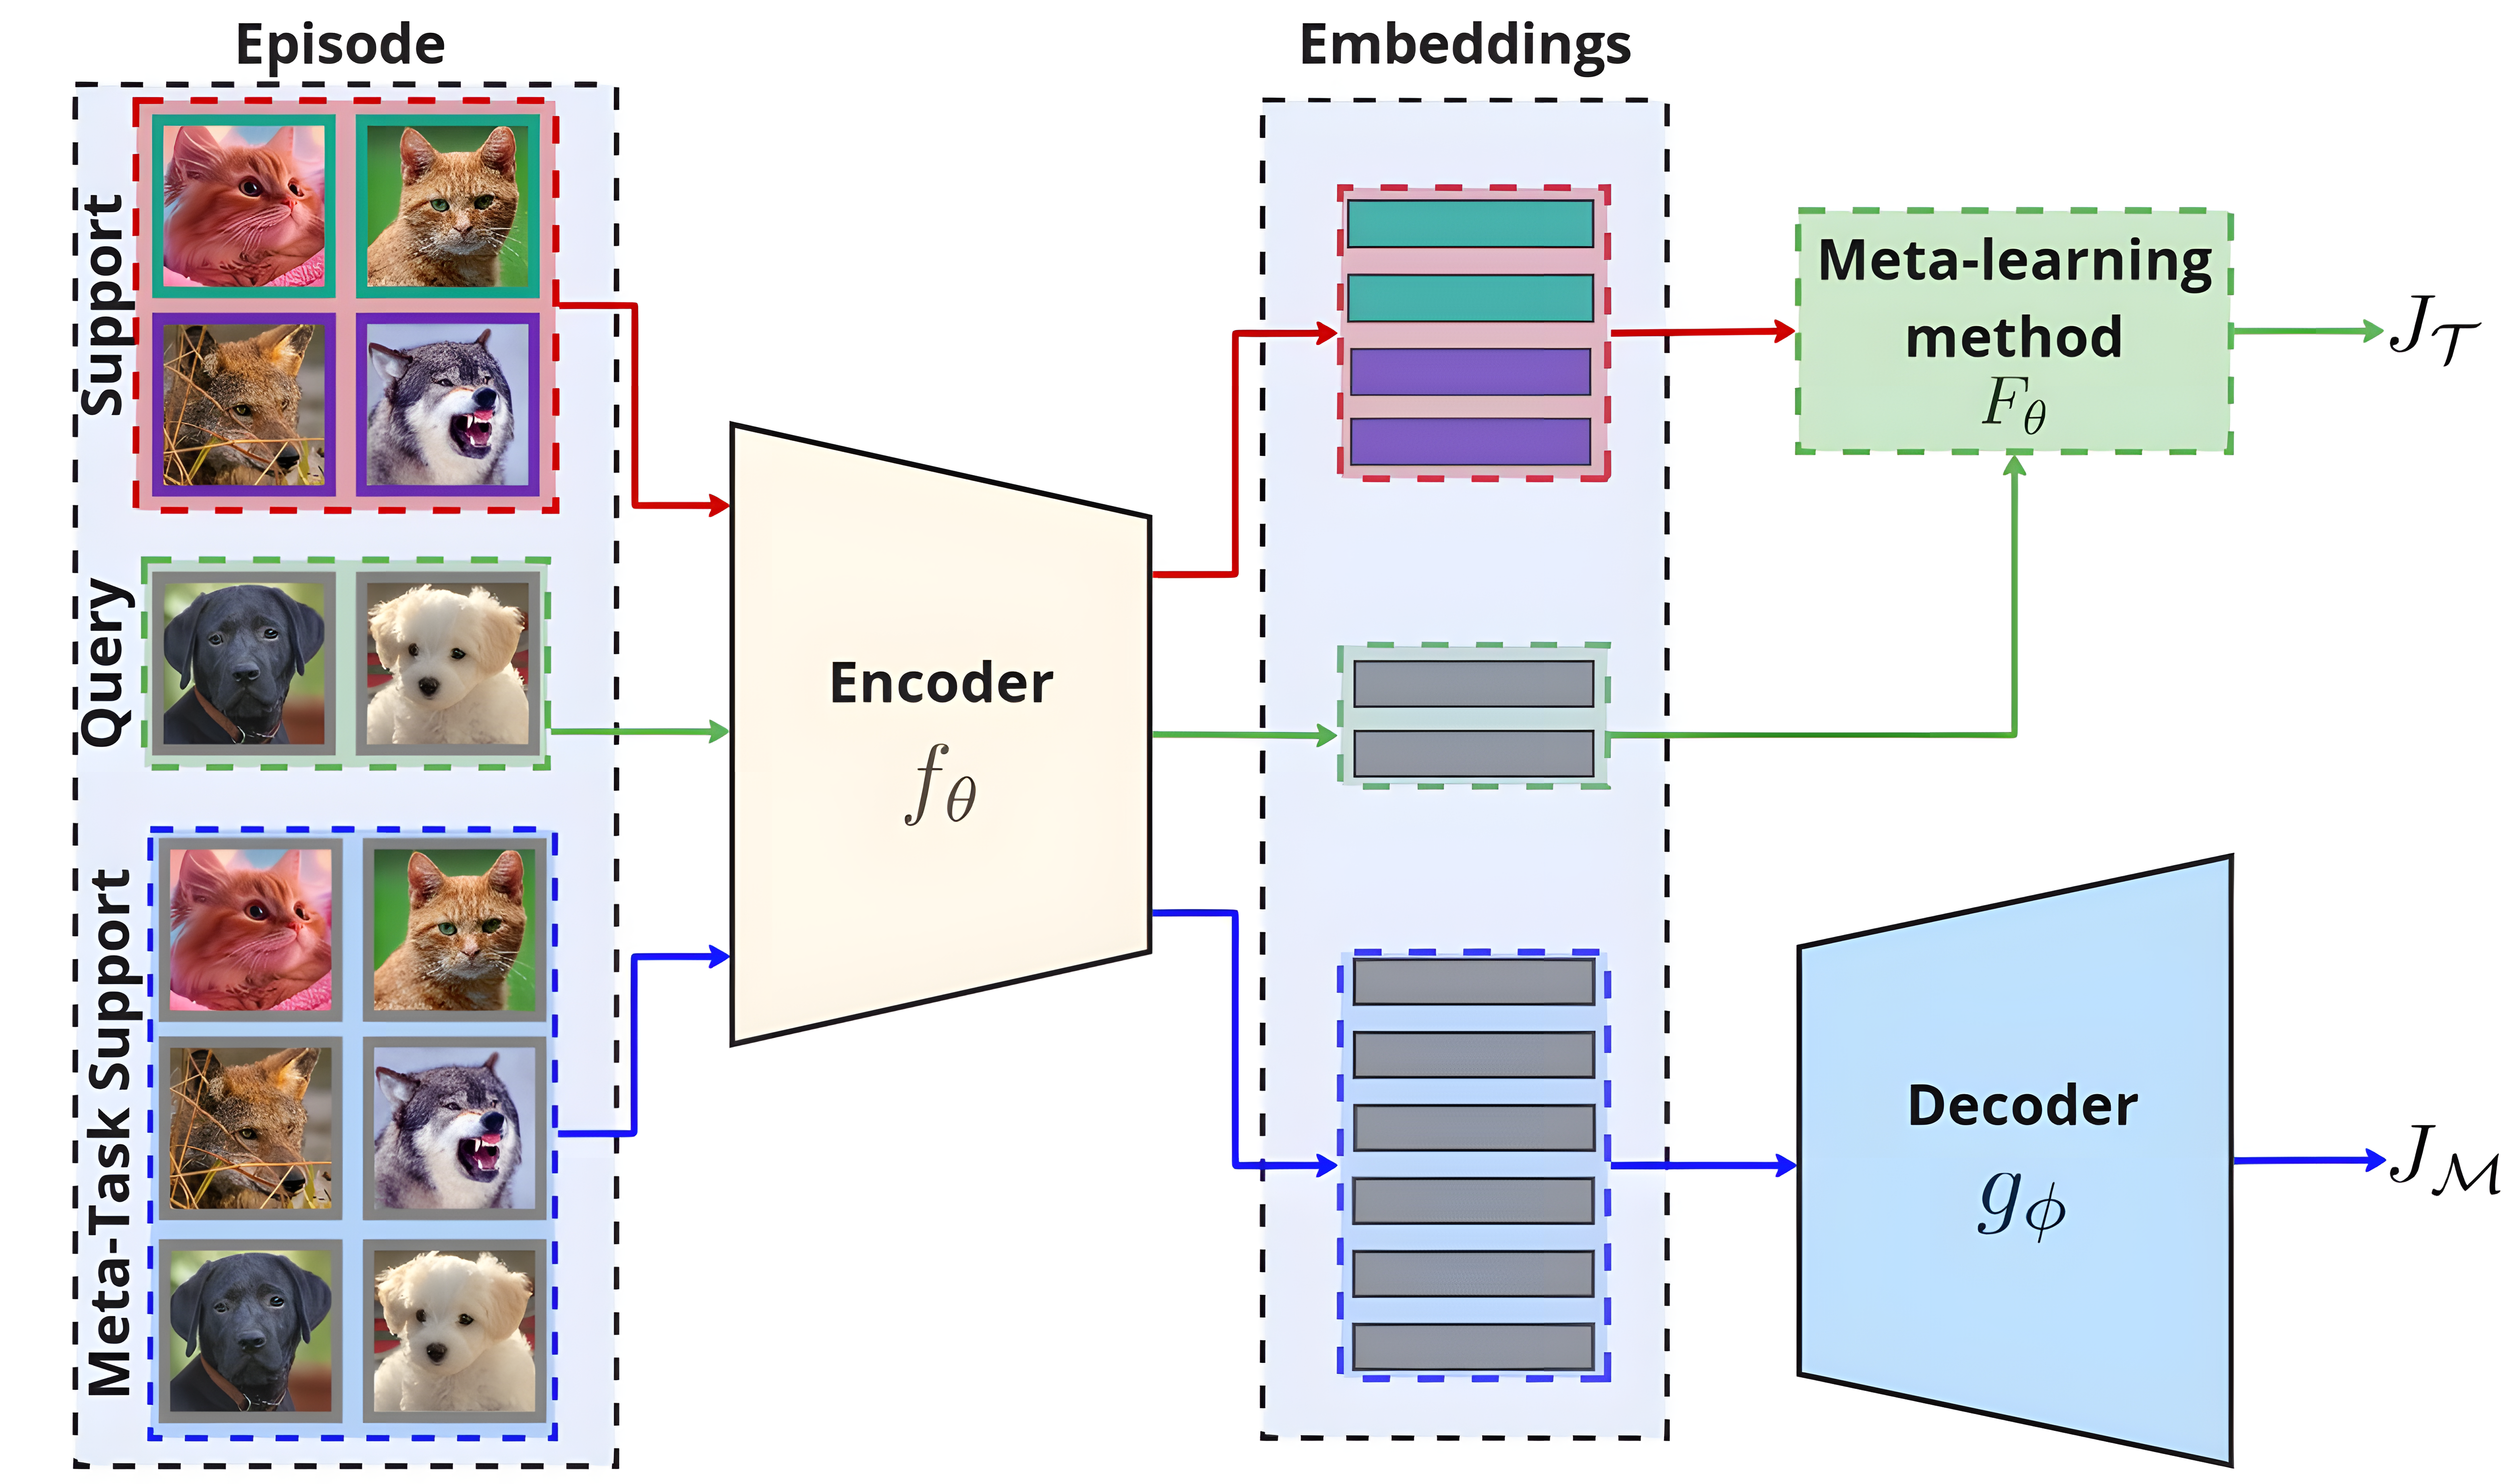
\includegraphics[width=\linewidth]{FIGURES/metatask/meta-tasks.png}   \caption{Detailed architecture of the Task-Decoder within the Meta-Task framework. The Meta-Task support set consists of unlabeled copies of support and query samples, which are fed into an encoder \( f_{\theta} \) to produce feature embeddings. These embeddings serve two key functions: (1) they are passed to a decoder \( g_{\phi} \) to reconstruct the input images, aiding in the learning of rich, meaningful representations, and (2) they are used to generate the meta-learning method ($F_{\theta}$) for query image classification. The model optimizes two objectives: classification loss (\( J_{\mathcal{T}} \)) and reconstruction loss (\( J_{\mathcal{M}} \)), each with a dedicated backpropagation step. The overall training loss is \( J_{\mathcal{T}} + \lambda J_{\mathcal{M}} \), balancing both classification accuracy and representation learning. For a broader application, the decoder \( g_{\phi} \) could be replaced by one or more neural networks that solve various unsupervised tasks.}

   \label{fig:1}
\end{figure}

\subsection{Related Work}


This section briefly reviews the relevant literature on meta-learning and regularization issues. Regularization techniques have been developed to improve the generalization ability of meta-learning models. These techniques can be broadly classified into four specialized regularization techniques for meta-learning. 1. Explicit Regularization (ER) \cite{rajeswaran2019imaml,mrmaml,pan2021meta,wang2023improving}, 2. Episode Augmentation Regularization (EAR) \cite{yamaguchi2023regularizing, shu2023dac}, 3. Task Augmentation Regularization (TAR) \cite{yao2021meta,yao2021improving,rajendran2020meta}, 4. Adversarial Task Upsampling (ATU) \cite{wu2022adversarial}. 

The ER methods impose explicit regularization terms on the meta-learning update, such as Meta-Learning with Implicit Gradients (iMAML) \cite{rajeswaran2019imaml}, Meta-Learning without Memorization (MR-MAML) \cite{mrmaml}, and their combinations or extensions \cite{pan2021meta, wang2023improving}. These methods directly constrain the model optimization process, aiming to improve the generalization performance of meta-learning models. For instance, minimax-meta regularization \cite{wang2023improving}
combines two types of regularizations at the inner and outer levels to enhance the generalization performance of bi-level meta-learning.

The EAR approach controls the meta-training by modifying individual tasks through noise or mixup \cite{yamaguchi2023regularizing, shu2023dac}. By expanding the amount of training data available for sampling, data augmentation supports various aspects of the meta-learning pipeline. It can be applied to support data in the inner loop of fine-tuning and enlarge the pool of evaluation data to be sampled during training. 

TAR methods generate new tasks by interpolating between or augmenting existing tasks \cite{yao2021meta, rajendran2020meta}, aiming to expand the task distribution for more robust generalization. For instance, methods such as MetaMix \cite{chen2021metamix}, and Channel Shuffle \cite{yao2021improving} have been proposed to increase the dependence of target predictions on the support set and provide additional knowledge to optimize model initialization. ProtoDiff \cite{du2023protodiff} enhances prototypical networks through a task-guided diffusion process; by generating synthetic features conditioned on the task, ProtoDiff \cite{du2023protodiff} augments the support set and improves the robustness of prototypes, significantly boosting classification performance. Additionally, the ATU approach \cite{wu2022adversarial} seeks to generate tasks that match the true task distribution by maximizing an adversarial loss, thereby improving meta-testing performance and the quality of upsampled tasks. These task augmentation techniques are designed to enhance the generalization capability of meta-learning models by effectively expanding the task distribution and mitigating overfitting during meta-training.

Recent works like Meta-Baseline \cite{chen2021metamix} have advanced few-shot learning by bridging transfer learning and meta-learning through pre-training feature extractors on base classes before few-shot fine-tuning, demonstrating that high-quality feature representations can sometimes eliminate the need for complex meta-learning algorithms. However, in contrast to Meta-Baseline's reliance on large-scale pre-training and ProtoDiff's \cite{du2023protodiff} computationally intensive task-guided diffusion models, our method learns robust embeddings during meta-training itself, making it more feasible for resource-constrained environments while remaining computationally efficient and method-agnostic.

In contrast to these methods, our proposed framework aims to regularize meta-learning tasks by introducing Meta-Tasks—auxiliary tasks designed to refine hidden representations without relying on extensive pre-training or synthetic data generation. Table \ref{tab:meta_learning_comparison} summarizes the key differences between various methods and our approach. We integrate an unsupervised autoencoder, specifically the Task-Decoder, directly within the meta-learning framework to provide continuous, unsupervised regularization during training. This helps prevent overfitting and improves generalization in an end-to-end manner.

By treating regularization as a learnable task, our framework enhances adaptability and generalization capabilities in a lightweight manner. It is suitable for a broader range of real-world applications where computational resources and labeled data are limited.

Meta-Task distinguishes itself from prior FSL approaches by introducing a learnable, task-specific regularization strategy that dynamically adapts to each task without modifying the underlying FSL architecture. Unlike LEO and iMAML, which focus on optimizing meta-initialization and gradient regularization, Meta-Task directly integrates into the optimization process through a parameterized neural layer $\phi$, learning task-adaptive constraints rather than enforcing fixed optimization heuristics. Unlike Wertheimer et al. \cite{wertheimer2021few} and Nag et al. \cite{nag2023reconstruction}, which utilize reconstruction-based self-supervision, our method does not rely on reconstruction loss. Furthermore, unlike Gidaris et al. \cite{gidaris2019boosting}, which introduces auxiliary tasks, Meta-Task requires neural layer $\phi$, instead only relying on better updates using self-supervised or semi-supervised tasks.

Our comprehensive experiments focus on fundamental meta-learning models (Prototypical Networks, MAML, MetaOptNet, and P$>$M$>$F~\cite{pmf}) that represent diverse approaches in the field. While some baseline comparisons were conducted with adjusted experimental settings (reduced batch sizes, modified query shots, etc.) due to computational constraints, our results consistently demonstrate the effectiveness of our Meta-Task framework across different meta-learning paradigms, validating its method-agnostic nature and broad applicability.

\begin{table}[ht]
\centering
\resizebox*{0.75\textwidth}{!}{
\begin{tabular}{lccccc}
\toprule
\textbf{Method} & \textbf{Category} & \textbf{Method-Agnostic} & \textbf{Complexity} \\
\midrule
\textbf{iMAML} \cite{imaml} & ER & No & High
\\
\textbf{MR-MAML} \cite{mrmaml} & ER & No & High \\ 
\textbf{Minimax-Meta} \cite{wang2023improving} & ER & No & Low \\
\textbf{DAC-MR} \cite{shu2023dac} & EAR & Yes & Medium \\
\textbf{MetaMix} \cite{chen2021metamix} & EAR & Yes & Medium \\
% \textbf{Channel Shuffle} \cite{yao2021improving} & TAR & Yes & Low \\
\textbf{ProtoDiff} \cite{du2023protodiff} & TAR & No & High \\
\textbf{ATU} \cite{wu2022adversarial} & TAR & Yes & High \\
\textbf{LEO} \cite{rusu2018meta} & ER & No & High \\
\textbf{Task-Decoder (Ours)} & \textbf{MTR} & \textbf{Yes} & \textbf{Medium} \\
\bottomrule
\end{tabular}
}
\caption{Comparison of meta-learning regularization methods. The table compares various meta-learning regularization techniques by category, method-agnostic capability, and computational complexity. Categories include Explicit Regularization (ER), Episode Augmentation Regularization (EAR), Task Augmentation Regularization (TAR), and our proposed Meta-Task Regularization (MTR).}
\label{tab:meta_learning_comparison}

\end{table}

\subsection{Meta-Task Framework}\label{sec:approach}
In this section, we introduce our proposed Meta-Task Framework, a novel approach that enhances generalization by integrating learnable Meta-Tasks as a form of regularization. By treating regularization itself as a learnable task, our framework encourages the model to develop richer and more robust feature representations. The framework is method-agnostic and can be seamlessly integrated with existing FSL models, such as Prototypical Networks and MAML. In the following subsections, we detail the components of the framework, including the Task-Decoder, the problem formulation, and the theoretical justification for its effectiveness.

Our framework extends MAML \cite{maml} by introducing regularization as a "learnable Meta-Task", enabling unsupervised task integration during meta-training without requiring additional data. The following subsections detail the implementation and theoretical foundations of our contributions:

\begin{itemize}
\item \textbf{Task-Decoder:} We introduce an unsupervised autoencoder architecture that implements our learnable regularization concept by reconstructing input images from their embeddings, proving its effectiveness in enriching feature representations.
\item \textbf{Problem Formulation:} We present the mathematical framework that enables the integration of unsupervised auxiliary tasks with existing FSL methods, demonstrating how our approach remains method-agnostic through separable loss functions.
\item \textbf{Theoretical Analysis:} We provide theoretical justification for our framework's convergence properties and establish how the joint optimization of primary and Meta-Tasks enhances generalization capabilities.
\end{itemize}

\subsubsection{Task-Decoder}

At the core of our Meta-Task Framework is the Task-Decoder (Figure \ref{fig:1}), an unsupervised learning component designed to enhance the embedding space by reconstructing input images from their embeddings. The Task-Decoder employs an autoencoder architecture, where the encoder \( f_{\theta} \) maps the input images to a latent embedding space, and the decoder \( g_{\phi} \) reconstructs the images from these embeddings.

By encouraging the embeddings to retain sufficient information for accurate reconstruction, the Task-Decoder prevents the encoder from focusing solely on discriminative features that may not generalize well. This leads to richer and more robust feature representations, ultimately improving the model's performance on unseen tasks.

The Task-Decoder operates in parallel with the primary few-shot learning model, processing the same inputs and contributing to the overall learning objective through its reconstruction loss.

\subsubsection{Problem Formulation}

Let the Meta-Task $\mathcal{M}$ denote the Task-Decoder, and our meta-learning method $F$ be Prototypical Networks. We define the encoder network \( f_{\theta} \) parameterized by \( \theta \), and \( g_{\phi} \) represent the decoder network parameterized by \( \phi \). 

For a given query sample \( x\in\mathcal{Q} \) and its true class \( y \) belonging to task $\mathcal{T}$, the Prototypical Network $F_{\theta}$ computes class prototypes using support set $\mathcal{S}$ and classifies $x$ based on the closest prototype to the embedding $f_{\theta}$.

\noindent
\textbf{Primary Task Loss:} The probability of \( x \) belonging to class \( n \) is:

\begin{equation} p_{\theta}(y={n} \mid x) = \frac{\exp\left(-d\left(f_{\theta}(x), c_{{n}}\right)\right)}{\sum_{k=1}^{N} \exp\left(-d\left(f_{\theta}(x), c_k\right)\right)}, \end{equation}
where $N$ is the number of tasks in the episode, \( c_n \) is the prototype of class \( n \) and \( d(\cdot, \cdot) \) denotes the Euclidean distance. The classification loss is then:

\begin{equation}
J_{\mathcal{T}}(x, \theta) = -\log p_{\theta}(y = n \mid x).
\end{equation}

\noindent
\textbf{Meta-Task Loss:} The Task-Decoder aims to reconstruct \( x \) from \( f_{\theta} \), with the reconstruction loss defined as:

\begin{equation}
J_{\mathcal{M}}(x, \theta, \phi) = \left\| g_{\phi}(f_{\theta}(x)) - x \right\|^2.
\end{equation}

\noindent
\textbf{Combined Loss Function:} The total loss for a sample \( x \) is a weighted sum of the primary task loss and the Meta-Task loss:

\begin{equation}
J(x, \theta) = J_{\mathcal{T}}(x, \theta) + \lambda J_{\mathcal{M}}(x, \theta, \phi),
\end{equation}
where \( \lambda \) is a hyperparameter balancing the two losses or the learning rate for the Meta-Task update.

\noindent
\textbf{Optimization:} The model parameters \( \theta \) and \( \phi \) are optimized jointly over all tasks and samples. For a given task $\mathcal{T}$, the overall loss is calculated by summing the combined losses over all query samples:

\begin{equation}\label{eq:task_loss}
J_{\mathcal{T}}(\theta) = \sum_{x \in \mathcal{T}} J_{\mathcal{T}}(x, \theta). 
\end{equation}

During meta-training, we sample a batch of tasks $\{\mathcal{T}_i\}^L_{i=1}$. The total loss across all tasks in an episode is:

\begin{equation}\label{eq:overall_loss_separate}
J(\theta) = \sum_{i=1}^{L} \left(J_{\mathcal{T}_i}(\theta) + \lambda J_{{\mathcal{M}_i}}(\theta, \phi)\right).
\end{equation}

By minimizing this combined loss, the model learns embeddings that are both discriminative for classification and informative for reconstruction, enhancing generalization across tasks. The full algorithm of the Task-Decoder integration is provided in Algorithm~\ref{alg:task_decoder}.

We define tasks and Meta-Tasks as separable if their loss functions can be computed independently and summed without including interaction terms. This structure allows us to optimize each component separately while still contributing to the overall objective. If the regularization term is separable (as in our case with the autoencoder), we can simplify \eqref{eq:overall_loss_separate} as
\begin{equation}\label{eq:9}
J(\theta) = \sum_{i=1}^{L} J_{\mathcal{T}_i}(\theta) +\lambda\sum_{i=1}^{L}J_{{\mathcal{M}_i}}(\theta,\phi).
\end{equation}

If each task may have multiple or no Meta-Tasks attached, the overall loss function generalizes to:
\begin{equation}\label{eq:10}
J(\theta) = \sum_{i=1}^{L} J_{\mathcal{T}_i}(\theta) +\lambda\sum_{r=1}^{R}J_{{\mathcal{M}_r}}(\theta,\phi),
\end{equation}
where $R$ is the total number of regularizers applied to the model.

\subsubsection{Justification}

Our Meta-Task framework provides unique theoretical guarantees, distinguishing it from existing regularization approaches. In Equations \eqref{eq:9} and \eqref{eq:10}, we demonstrated that incorporating auxiliary tasks into training effectively reformulates the FSL paradigm to a new FSL setting with a combined distribution of primary tasks and Meta-Tasks, denoted as 
$\mathcal{T}'$. This reformulation allows the overall training objective to be expressed as a sum over $L+R$ tasks, preserving the structure necessary for standard FSL optimization techniques.

When using MAML as the FSL method, based on convergence guarantees proven in literature~\cite{wang2022global}, our approach converges to an optimal set of parameters for $\mathcal{T}'$. Since the Meta-Tasks are carefully designed to enhance generalization, this optimal parameter set enables the model to generalize effectively across both primary tasks and Meta-Tasks. The convergence of $\phi$ to its global optima further ensures that the learned embeddings retain the essential information necessary for both classification and reconstruction. This joint optimization ($\theta$) constructs a globally optimal representation space, improving overall model performance on unseen tasks by reducing generalization error.

A critical advantage of Meta-Task is the separability of the primary and auxiliary tasks. Since their loss functions can be computed independently, optimization can proceed efficiently, with each task contributing to the overall objective. This design simplifies the optimization process and supports convergence to a global optimum, as the auxiliary tasks act as an implicit regularizer, reducing overfitting by penalizing non-generalizable embeddings.

A rigorous mathematical proof is more challenging for FSL methods beyond MAML. However, as all FSL methods aim to optimize parameters that generalize across task distributions with limited examples, it is reasonable to infer that our approach improves generalization capabilities, as demonstrated in the results section. In the supplementary material, we provide additional experiments, including visualizations of reconstructed features, to empirically validate how Meta-Task enhance embedding quality and task generalization.

\begin{remark}{The proposed regularization approach is method-agnostic and can be applied to any FSL learning method.} \end{remark}
\begin{remark}{Equations \eqref{eq:9}, \eqref{eq:10} hold only if tasks and Meta-Tasks are separable or independent.}
\end{remark}
\begin{remark}{The use of autoencoders is because autoencoders can be used with any type of data, are easy to use, and are flexible in architecture.}
\end{remark}

\begin{algorithm}[t]
  \caption{Meta-Tasks: Task-Decoder}
  \label{alg:task_decoder}
  \begin{enumerate}
      \item \textbf{Require:} Distribution over tasks $p(\mathcal{T})$; \\
      \item \textbf{Require:} embedding network $f_{\theta}$; \\
      \item \textbf{Require:} decoder network $g_{\phi}$; \\
      \item \textbf{Require:} learning rates $\alpha$, $\lambda$; 
      \item \textbf{Require:} meta-learning method $F$ (e.g., Prototypical Networks); 
      \item \textbf{Require:} classification loss $J_{\mathcal{T}}(x, \theta)$;
      \item \textbf{Require:} reconstruction loss $J_{\mathcal{M}}(x, \theta, \phi) = \| g_{\phi}(f_{\theta}(x)) - x \|^2$ \\
      \item Randomly initialize $\theta$ and $\phi$
      \item \textbf{while} not done \textbf{do}
      \begin{enumerate}
          \item Sample support set $\mathcal{S} \sim p(\mathcal{T})$
          \item Sample query set $\mathcal{Q} \sim p(\mathcal{T})$
          \item Compute reconstruction loss: \\
          $J_{\mathcal{M}}(\theta, \phi) \leftarrow \frac{1}{|\mathcal{S} \cup \mathcal{Q}|} \sum_{x \in \mathcal{S} \cup \mathcal{Q}} J_{\mathcal{M}}(x, \theta, \phi)$
          \item Use support set $\mathcal{S}$ and embedding network $f_{\theta}$ to obtain meta-learning method $F_{\theta}$
          \item Compute classification loss on query set: \\
          $J_{\mathcal{T}}(\theta) \leftarrow \frac{1}{|\mathcal{Q}|} \sum_{x \in \mathcal{Q}} J_{\mathcal{T}}(x, F_{\theta})$
          \item Update embedding network parameters: \\
          $\theta \leftarrow \theta - \alpha \nabla_{\theta} \left( J_{\mathcal{T}}(\theta) + \lambda J_{\mathcal{M}}(\theta, \phi) \right)$
          \item Update decoder parameters: \\
          $\phi \leftarrow \phi - \lambda \nabla_{\phi} J_{\mathcal{M}}(\theta, \phi)$
      \end{enumerate}
      \item \textbf{end while}
  \end{enumerate}
  \end{algorithm}


\subsection{Experiments and Results}\label{sec:results}

In this section, we conduct comprehensive experiments to validate the effectiveness of our proposed {Meta-Task} framework in enhancing generalization and mitigating overfitting in few-shot learning. Our objectives are to: 
\begin{enumerate} 
\item Demonstrate that incorporating Meta-Tasks as auxiliary regularization improves model generalization to both seen and unseen tasks.
\item Validate that leveraging both labeled and unlabeled data through an unsupervised autoencoder refines hidden representations.
\item Showcase the method-agnostic applicability of {Meta-Task} across various FSL settings and its practical efficiency in resource-constrained scenarios. 
\end{enumerate}
  
We begin by outlining the experimental setup, including datasets, model architectures, and implementation specifics. Following this, we present our results along with a comprehensive analysis of our findings, focusing on the impact of the {Meta-Task} framework on performance, convergence speed, and variance reduction.
  
\subsubsection{Datasets}
  
We evaluated the proposed {Meta-Task} framework on three standard benchmarks commonly used in few-shot learning:

\noindent
\textbf{MiniImageNet}~\cite{mini-imagenet}: This dataset consists of 100 classes selected from ImageNet, with 600 images per class resized to $84 \times 84$ pixels. It is divided into 64 training, 16 validation, and 20 test classes, ensuring that test classes are entirely disjoint from training classes for robust evaluation of generalization capabilities.

\noindent
\textbf{TieredImageNet}~\cite{ren2018meta}: A larger and more challenging dataset comprising 608 classes organized into 34 high-level categories, providing semantic diversity. It includes 351 training, 97 validation, and 160 test classes, with images resized to $84 \times 84$ pixels. Its hierarchical structure makes it suitable for evaluating models' ability to generalize across different levels of abstraction.

\noindent
\textbf{FC100}~\cite{oreshkin2018tadam2}: Derived from the CIFAR-100 dataset, FC100 contains 100 classes, each with 600 images resized to $32 \times 32$ pixels. The dataset is split into 60 training, 20 validation, and 20 test classes. It presents unique challenges due to low-resolution images and high intra-class variability, making it an excellent benchmark for assessing model robustness.
  
These datasets offer diverse and challenging scenarios for few-shot learning, enabling us to thoroughly evaluate the generalization capabilities of the {Meta-Task} framework.
  
\subsubsection{Methods}
  
To demonstrate the method-agnostic nature of our approach, we integrated the {Meta-Task} framework with four few-shot learning models:

\noindent
\textbf{Prototypical Network (PN)} \cite{snell2017prototypical}: Utilizes a ResNet-50 \cite{resnet-code} backbone for feature extraction. It computes class prototypes in the embedding space, classifying query samples based on their distances to these prototypes.

\noindent
\textbf{MAML}~\cite{maml}: Employs a four-layer ConvNet architecture aiming to find initial model parameters that can be quickly adapted to new tasks with minimal gradient updates.

\noindent
\textbf{MetaOptNet}~\cite{lee2019metaoptnet}: Uses a ResNet-12 backbone and incorporates differentiable convex optimization layers for efficient classification, seamlessly integrating with our {Meta-Task} framework.

\noindent
\textbf{P$>$M$>$F} \cite{pmf}: Uses DINO\cite{dino} framework as its backbone. Like PN, it computes class prototypes in the embedding space. It classifies query samples based on their distances to these prototypes but with the added benefit of leveraging pre-trained transformer-based feature extraction.

In our {Meta-Task} framework, we introduced a Task-Decoder employing an unsupervised autoencoder to reconstruct input images from their embeddings. The decoder mirrors the encoder architecture used in the backbone models. This process leverages both labeled and unlabeled data (support and query sets), refining the hidden representations and mitigating overfitting.

For the autoencoder architecture, we experimented with different configurations to assess the impact of the Task-Decoder's depth on performance. Specifically, we used both shallow and deep autoencoders, with parameters ranging from 75K to 250K. The shallow autoencoder consists of two convolutional layers, while the deep autoencoder includes four convolutional layers. This allowed us to analyze how the complexity of the Task-Decoder affects the overall performance.

We trained all models using the Adam optimizer with learning rates set to $1 \times 10^{-4}$ for the encoder and classifier, and $1 \times 10^{-6}$ for the Task-Decoder. Each model was trained over 50,000 episodes using 5-way 1-shot and 5-way 5-shot scenarios. The query size was maintained at 15 for both training and evaluation phases. To enhance model robustness, we applied standard data augmentation techniques, including random cropping, horizontal flipping, and color jittering.

Furthermore, we investigated the effect of using multiple autoencoders per task by associating different autoencoders with specific layers of the encoder network. However, we found that using a single autoencoder provided a good trade-off between performance improvement and computational overhead. The complete source code and results for this paper can be found in the following GitHub repository: \href{https://github.com/woreom/meta-learning}{https://github.com/woreom/meta-learning}.
  

\begin{figure}
  
  \centering
    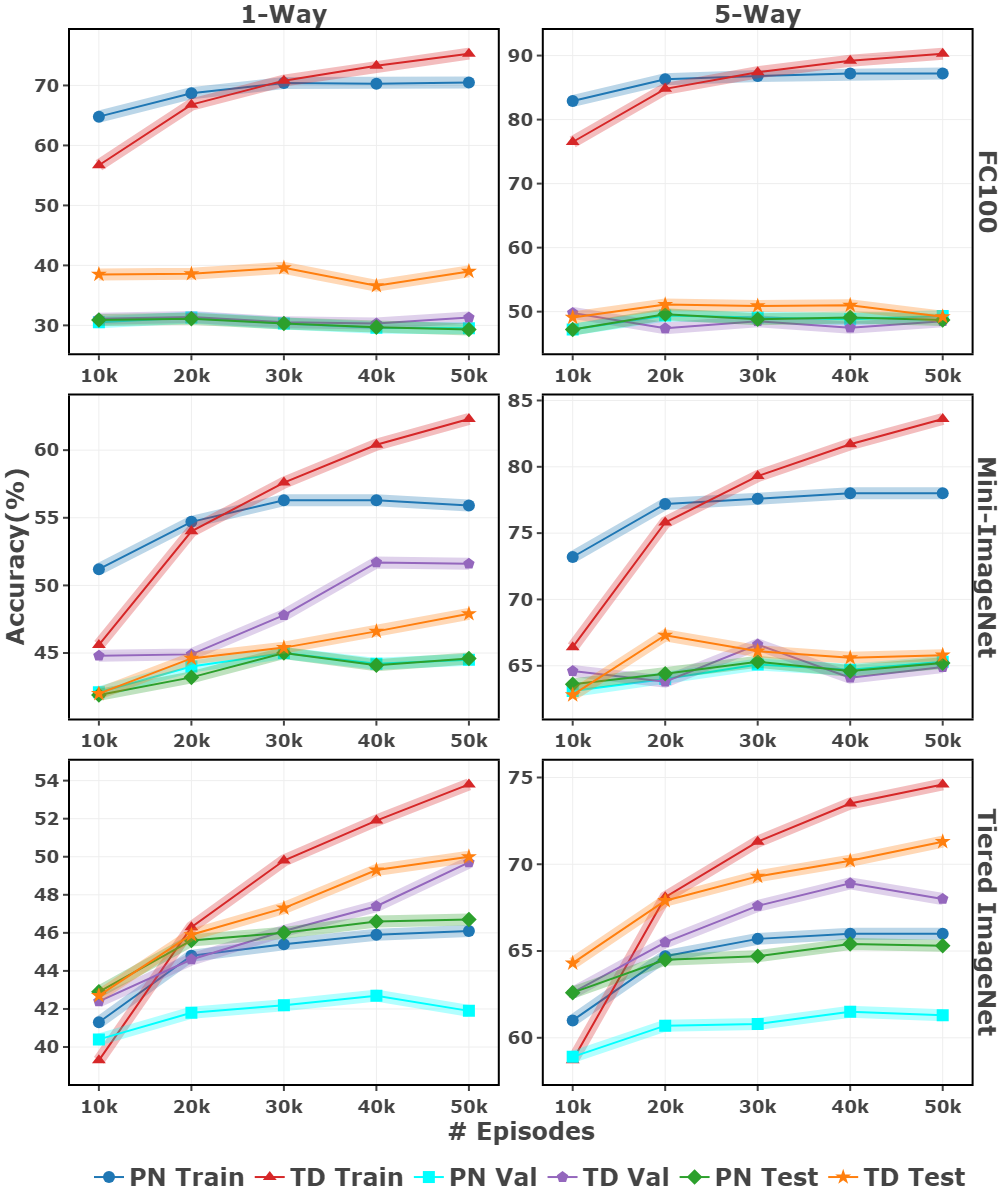
\includegraphics[width=0.9\linewidth]{FIGURES/metatask/acc_2.png}
    \caption{Accuracy curves for Prototypical Networks (PN) and Task-Decoder (TD) across different datasets, plotted against the number of episodes.}
    \label{fig:5}
\end{figure}

\begin{figure}
    \centering
     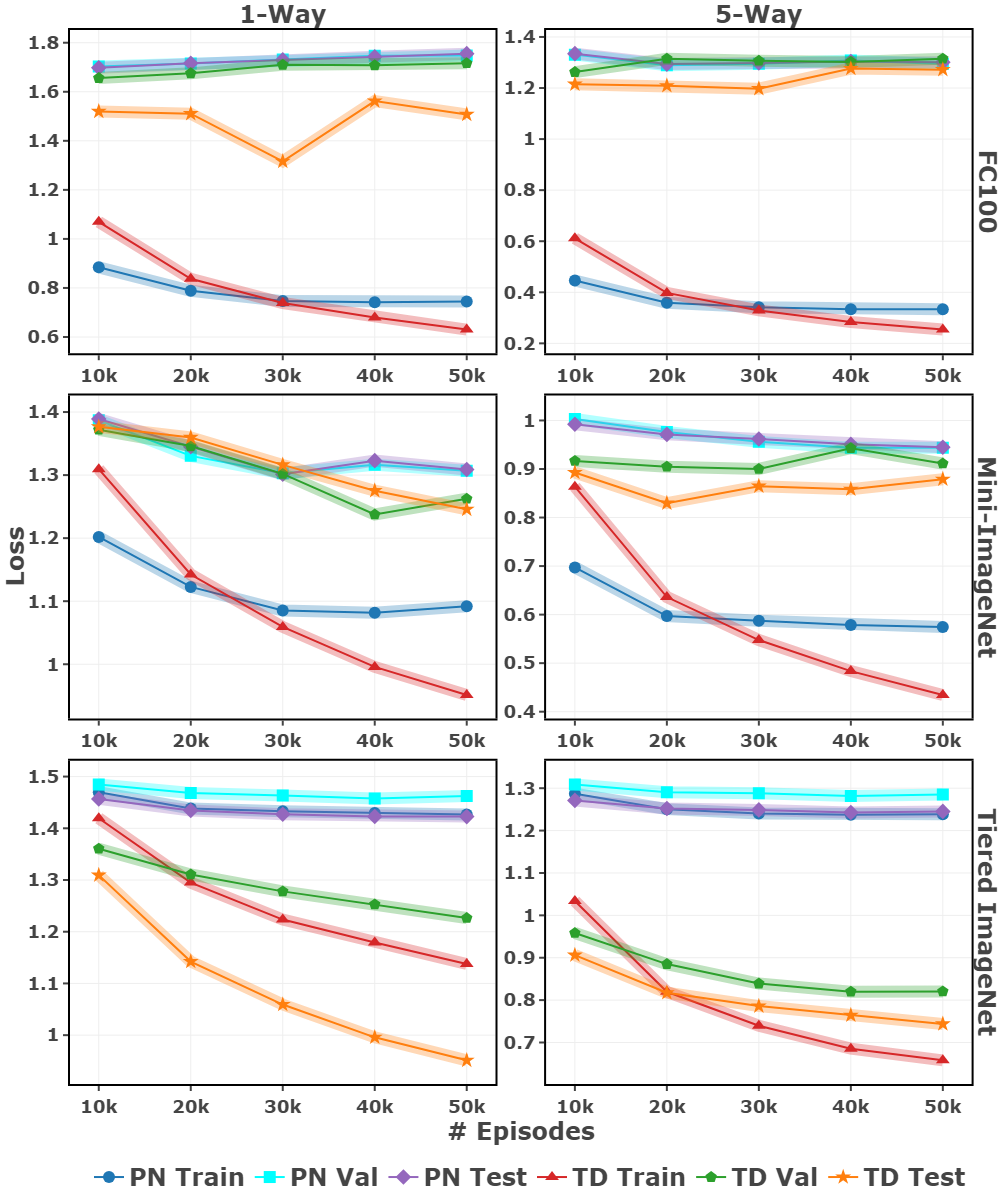
\includegraphics[width=0.9\linewidth]{FIGURES/metatask/loss_2.png}
     \caption{Loss curves for Prototypical Networks (PN) and Task-Decoder (TD) across different datasets, plotted against the number of episodes.}
     \label{fig:4}
  \end{figure}

  \begin{table}[!htbp]
    \centering
    \resizebox*{!}{0.4\linewidth}{
    \begin{tabular}{ll|cccc}
                                                    &                    & \multicolumn{2}{c}{MiniImageNet}                                        & \multicolumn{2}{c}{TieredImageNet}                                          \\
    Method                                         & Backbone           & \multicolumn{1}{l}{5-way 1-shot(\%)} & \multicolumn{1}{l}{5-way 5-shot(\%)} & \multicolumn{1}{l}{5-way 1-shot(\%)} & \multicolumn{1}{l}{5-way 5-shot(\%)} \\
    \hline
    PN                           & ResNet18           & 45 ± 0.0                         & 65.2 ± 0.0                           & 46.6 ± 0.0                           & 65.4 ± 0.0                           \\
    \textbf{PN(TD)}              & ResNet18           & \textbf{47.9 ± 0.0}              & \textbf{66.1 ± 0.0}                  & \textbf{50 ± 0.0}                    & \textbf{71.3 ± 0.0}                  \\
    MAML                         & CNN                & 47.54                            & 62.23                                & -                                    & -                                    \\
    \textbf{MAML (TD)}           & Shallow CNN Decoder& \textbf{47.81}                   & \textbf{62.52}                       & -                                    & -                                    \\
    \textbf{MAML (TD)}           & CNN                & \textbf{47.67}                   & \textbf{63.01}                       & -                                    & -                                    \\
    Relation Networks\cite{sung2017learning}      & 64-96-128-256      & 50.44 ± 0.82                     & 65.32 ± 0.70                         & 54.48 ± 0.93                         & 71.32 ± 0.78                         \\
    R2D2\cite{bertinetto2018meta}        & 96-192-384-512     & 51.2 ± 0.6                       & 68.8 ± 0.1                           & -                                    & -                                    \\
    Transductive Prop Nets\cite{liu2018learning} & 96-192-384-512     & 55.51 ± 0.86                     & 69.86 ± 0.65                         & 59.91 ± 0.94                         & 73.3 ± 0.75                          \\
    SNAIL\cite{mishra2017simple}         & ResNet-12          & 55.71 ± 0.99                     & 68.88 ± 0.92                         & -                                    & -                                    \\
    AdaResNet\cite{munkhdalai2018rapid} & ResNet-12          & 56.88 ± 0.62                     & 71.94 ± 0.57                         & -                                    & -                                    \\
    TADAM\cite{oreshkin2018tadam2}      & ResNet-12          & 58.5 ± 0.30                      & 76.7 ± 0.30                          & -                                    & -                                    \\
    MetaOptNet                   & ResNet-12          & 61.23 ± 0.29                     & 77.14 ± 0.21                         & 63.10 ± 0.34                         & 78.58 ± 0.27                         \\
    \textbf{MetaOptNet (TD)}     & ResNet-12          & \textbf{61.35 ± 0.29}            & \textbf{77.3 ± 0.22}                 & \textbf{63.20 ± 0.34}                & \textbf{78.66 ± 0.27}                \\
    \textbf{P$>$M$>$F}           & IN1K,ViT-base       & \textbf{72.80 ± 0.0}             & \textbf{90.70 ± 0.0}                 & -                                    & -                                    \\
    \textbf{P$>$M$>$F(TD)}       & IN1K,ViT-base       & \textbf{74.10 ± 0.0}             & \textbf{92.30 ± 0.0}                 & -                                    & -                                    \\
    \hline
    \end{tabular}}
    \caption{Comparison of few-shot classification accuracies (\%) with 95\% confidence intervals on MiniImageNet and TieredImageNet datasets. Results are reported for 5-way 1-shot and 5-way 5-shot. `PN` and `TD` refer to Prototypical Networks and Task-Decoder, respectively.}
    \label{table:1}
  \end{table}


  \begin{table}[!htpb]
  \centering
  \resizebox*{!}{0.25\linewidth}{\begin{tabular}{l|cc}
                                                &  \multicolumn{2}{c}{FC100}                                                   \\
  Method                                         & \multicolumn{1}{l}{5-way 1-shot(\%)} & \multicolumn{1}{l}{5-way 5-shot(\%)} \\
  \hline & & \\
  PN                            & 31.1 ± 0.0                           & 49.6 ± 0.0                           \\
  \textbf{PN (TD)}  & \textbf{39 ± 0.0}                    & \textbf{51.1 ± 0.0}                  \\
  TADAM\cite{oreshkin2018tadam2}                  & 40.1 ± 0.4                           & 56.1 ± 0.4                           \\
  MetaOptNet                                     & 40.19 ± 0.25                         & 55.04 ± 0.26                         \\
  \textbf{MetaOptNet (TD)}             & \textbf{40.59 ± 0.26}                & \textbf{55.38 ± 0.25}                \\
  \hline
  \end{tabular}}
  \caption{Comparison of few-shot classification accuracies (\%) with 95\% confidence intervals on the FC100 dataset \cite{oreshkin2018tadam2}. Results are reported for 5-way 1-shot and 5-way 5-shot settings. `PN' and `TD' refer to Prototypical Networks and Task-Decoder, respectively.}
  \label{table:2}
  \end{table}

\subsubsection{Performance Evaluation}

Our experimental results demonstrate that the Meta-Task framework consistently outperforms baseline models across all datasets and settings, achieving higher accuracy with significantly fewer training episodes. For example, as shown in Figure~\ref{fig:5}, TD enables higher test accuracy within 20k episodes, whereas PN Test fails to achieve the same even after 50k episodes. Similarly, in Table~\ref{table:1}, TD P$>$M$>$F reaches 92.30\% accuracy in 3k episodes compared to P$>$M$>$F's 90.70\% after 4k episodes.

These results highlight the framework's efficiency in leveraging a small number of additional parameters to enhance generalization while reducing computational overhead. By introducing Meta-Tasks, the learning process is effectively regulated, eliminating the need for extensive parameter tuning or large-scale episodic training. This makes the Meta-Task framework both lightweight and practical for real-world applications. Further details on are provided in Table~\ref{table:1} and Table~\ref{table:2}.
  
\textbf{Prototypical Network Results}
Table~\ref{table:1} presents our experimental results on MiniImageNet and TieredImageNet, where our proposed method, the Task-Decoder, demonstrates significant performance improvements over the baseline Prototypical Networks. Specifically, on TieredImageNet in the 5-way 5-shot setting, our approach achieved an increase from 65.4\% to 71.3\% in test set accuracy, reflecting a substantial 5.9\% absolute improvement. This gain indicates superior meta-generalization capabilities of our method.

In the 5-way 1-shot scenario, the Task-Decoder improved accuracy from 46.6\% to 50\% on TieredImageNet, highlighting its efficacy in scenarios with extremely limited data. These consistent improvements across different datasets and settings demonstrate the robustness and effectiveness of our approach.

\textbf{MAML Results}
Table~\ref{table:1} also showcases the performance of the {Task-Decoder} integrated with MAML. Our method outperforms the baseline MAML by an average of 0.48\% in the 5-way 1-shot setting and 0.78\% in the 5-way 5-shot setting on MiniImageNet. Although the absolute improvements are modest, they demonstrate the effectiveness of the {Task-Decoder} in enhancing the adaptability of MAML.
  
To examine the impact of the {Task-Decoder's} architecture ($\phi$) on generalization, we trained MAML using two different{Task-Decoders}: a shallow decoder with 75K parameters and a deeper decoder with 250K parameters. Interestingly, the shallow decoder excelled in the 5-way 1-shot task, suggesting that deeper models are not always superior when data is scarce. In contrast, the deeper decoder performed better with more shots, highlighting the importance of model depth in specific contexts. This indicates that the Task-Decoder and its Meta-Task extensions can be effective even with a shallow network, which is beneficial in resource-constrained environments.
  
It's important to note that MAML requires the computation of second derivatives during optimization. However, to remain consistent with our claim of a method-agnostic framework, we chose to use a first-order approximation for the Task-Decoder's optimization. This decision avoids the computational overhead associated with second-order derivatives but may introduce approximation errors. Another limitation may stem from the inherent difficulties of optimizing the learning rate in MAML, which is complicated by the need for careful tuning due to its sensitivity to hyperparameters. While using the same learning rate as the Prototypical Networks simplifies comparisons, it likely constrained MAML's overall performance. These factors suggest that further optimization and fine-tuning could enhance the benefits of integrating the Task-Decoder with MAML.
  
textbf{MetaOptNet Results}
The results presented in Table~\ref{table:1} indicate that integrating the Task-Decoder with MetaOptNet \cite{lee2019meta} leads to modest but consistent performance improvements, with an average accuracy increase of 0.12\% in the 5-way 1-shot setting and 0.16\% in the 5-way 5-shot setting on MiniImageNet. While these gains are not as pronounced as those observed with other methods, they underscore the potential of the Task-Decoder to enhance performance even in well-optimized frameworks like MetaOptNet.

We attribute the smaller improvements to MetaOptNet's distinctive training setup, where variations in batch size and the number of shots significantly impact model performance. Due to hardware limitations, we reduced the batch size and the number of training shots, which may have constrained the performance gains. These findings suggest that further hyperparameter optimization, such as adjusting batch size or learning rate, could yield more substantial improvements.

\textbf{P$>$M$>$F Results}

Due to the pre-trained nature of the encoder, we implemented a custom scheduler to align TD's optimization. Additionally, hardware constraints necessitated deviations from the original hyperparameters, such as reducing image sizes and query shots, which may have influenced the observed improvements. Despite these constraints, TD achieved a notable 1.45\% performance increase, demonstrating its flexibility and adaptability to transformer-based methods under constrained conditions.
  
\subsubsection{Regularization Improvements}

Figure~\ref{fig:5} illustrates that our method achieves higher accuracy more quickly during all training, validation, and testing phases compared to the baseline, which demonstrates faster convergence. Additionally, Figure~\ref{fig:4} illustrates that the loss associated with our method decreases more rapidly and consistently remains lower throughout the training process across all training, validation, and test sets. The Task-Decoder achieves a mean loss of 1.23 with a variance of 0.001, whereas the baseline has a mean loss of 1.3 and a variance of 0.0002. This indicates more efficient learning and improved generalization.
  
To address concerns regarding implementation specifics, we have provided detailed information about the hyperparameters, training times, and autoencoder architectures in the supplementary material. We also conducted ablation studies to analyze the effect of different autoencoder architectures and the use of multiple autoencoders per task. The results indicate that while deeper autoencoders can provide marginal performance gains, the computational overhead increases significantly. Therefore, a single, appropriately sized autoencoder strikes a good balance between performance and efficiency.
  
\subsection{Conclusion}

In this paper, we introduced the {\textbf{Meta-Task}} framework, a method-agnostic approach for regularization in few-shot learning (FSL) that leverages Meta-Tasks as auxiliary tasks with a set of parameters to mitigate overfitting. Theoretically, we demonstrated that our approach achieves global optima with strong generalization across tasks. Empirically, we validated its efficacy through the {\textbf{Task-Decoder}} Meta-Task, which significantly improved performance on MiniImageNet and TieredImageNet benchmarks, achieving faster convergence and reduced generalization error with minimal hyperparameter tuning. Overall, our findings highlight the potential of the {{Meta-Task}} framework to improve FSL models, suggesting that even minor adjustments can lead to significant benefits and encourage further exploration of Meta-Task-based regularization in broader contexts.

\section{Overall Findings}

Across the three core tasks—BEpiC, MetaRep, and Meta-Task—this chapter systematically advances the state of generalization in few-shot learning by addressing complementary challenges in episode generation, representation learning, and regularization. These contributions collectively demonstrate Stage 2 of our wireless foundation model framework: enabling rapid task adaptation with minimal labeled data.

\textbf{BEpiC} introduced binary episodes to improve cross-domain generalization, addressing the challenge of distribution shift between meta-training and meta-test tasks. By simplifying episodes to binary classification problems, BEpiC encourages learning of domain-invariant representations that transfer more robustly across different task distributions. For wireless foundation models, this translates to better generalization across SNR regimes, channel conditions, and potentially unseen modulation families—reducing the brittleness of models trained on fixed task distributions.

\textbf{MetaRep} demonstrated that leveraging both labeled and unlabeled data through episodic representation learning significantly enhances meta-learning performance. By learning task-conditioned feature modulations, MetaRep adapts representations dynamically based on the support set, enabling more effective few-shot classification. This aligns with the foundation model principle of learning general-purpose representations that can be rapidly specialized—Meta-Rep shows how to modulate pre-trained features for specific tasks without extensive retraining.

\textbf{Meta-Task} introduced method-agnostic learnable regularization, showing that adaptive regularization strategies improve few-shot generalization across diverse meta-learning algorithms. This finding is critical for foundation models, which must be robust to various deployment scenarios. Meta-Task's approach of learning when and how to regularize based on task characteristics provides a principled mechanism for ensuring reliable adaptation regardless of the specific meta-learner or downstream application.

\textbf{Collectively}, these contributions demonstrate that enhancing generalization in few-shot learning requires a holistic approach: (1) designing episodes that expose the learner to meaningful task diversity (BEpiC), (2) leveraging both labeled and unlabeled data to learn robust, adaptable representations (MetaRep), and (3) integrating adaptive, learnable regularization mechanisms (Meta-Task). The empirical results consistently show that each method yields measurable improvements in accuracy, robustness, and data efficiency, and that their principles are broadly applicable across meta-learning paradigms.

\textbf{Foundation Model Implications:} This chapter establishes meta-learning as the critical adaptation layer (Stage 2) in our wireless foundation model framework. Given pre-trained representations from DenoMAE (Chapter 2, Stage 1), these meta-learning techniques enable rapid specialization to new modulation classification tasks with minimal labeled samples. The ability to adapt quickly with few examples is the hallmark of foundation models—distinguishing them from traditional supervised approaches. BEpiC, MetaRep, and Meta-Task collectively demonstrate that wireless signals can exhibit this rapid adaptation capability, bridging the gap between general-purpose pre-training and task-specific deployment. The next chapter (Chapter 4) explores semi-supervised learning as a practical training methodology, and Chapter 5 integrates these adapted representations with LLMs to enable true open-set recognition—completing the wireless foundation model vision.
\chapter{Unlabeled Data Utilization through Semi-Supervised Learning}

\section{Introduction}

The abundance of unlabeled data in real-world scenarios presents both a challenge and an opportunity for modern machine learning systems and, critically, for foundation models. While supervised learning methods have achieved remarkable success, their reliance on large quantities of labeled data limits their applicability in domains where annotation is costly, time-consuming, or impractical. Semi-supervised learning (SSL) addresses this limitation by leveraging the vast pool of unlabeled data alongside a small set of labeled examples, enabling models to learn more robust and generalizable representations—precisely the data efficiency required for foundation model deployment.

For wireless foundation models, semi-supervised learning serves two essential purposes. First, it provides a practical training methodology that reduces the labeled data requirements during the pre-training stage (Chapter 2), allowing models like DenoMAE to learn from massive unlabeled signal datasets with minimal supervision. Second, it enables efficient fine-tuning during the adaptation stage (Chapter 3), where meta-learning techniques can be enhanced with semi-supervised objectives to maximize utilization of available unlabeled signals in deployment environments.

This chapter explores advanced semi-supervised learning techniques designed to maximize the utility of unlabeled data, with particular focus on their application in classification tasks. We discuss the theoretical foundations of SSL, review state-of-the-art methods such as pseudo-labeling, consistency regularization, and self-supervised pretext tasks, and highlight their strengths and limitations in data-constrained environments. Furthermore, we introduce \textbf{RLPL (Representation Learning with Pseudo-Labeling)}—our novel approach that integrates improved representation learning and pseudo-labeling strategies, demonstrating effectiveness in enhancing classification accuracy and generalization with limited labeled data.

Through comprehensive experiments and analysis, we show how the proposed methods bridge the gap between supervised and unsupervised learning, offering practical solutions for scenarios where labeled data is scarce but unlabeled data is plentiful. For wireless foundation models, this paradigm is critical: spectrum monitoring generates continuous streams of unlabeled signals, but obtaining expert-labeled modulation classifications at scale is prohibitively expensive. RLPL enables foundation models to learn effectively from this imbalanced data distribution.

\textbf{Foundation Model Context:} This chapter complements Chapters 2 and 3 by providing the practical training methodology that makes wireless foundation models viable. Chapter 2 introduced self-supervised pre-training (Stage 1); Chapter 3 introduced meta-learning for rapid adaptation (Stage 2); this chapter demonstrates how semi-supervised learning enhances both stages by maximizing unlabeled data utilization. Together, these techniques enable the three-stage wireless foundation model framework: (1) pre-train on unlabeled signals via masked autoencoders, (2) adapt rapidly with meta-learning using small labeled sets augmented by semi-supervised objectives, and (3) integrate with LLMs for open-set recognition (Chapter 5). The insights and techniques presented in this chapter contribute to developing flexible, data-efficient machine learning frameworks capable of adapting to a wide range of real-world wireless challenges.

\subsection{Semi-Supervised Learning: An Overview}

At its core, semi-supervised learning seeks to improve model performance beyond what is achievable with the limited labeled data alone by exploiting the information latent within the abundant unlabeled data. The fundamental principle is that the structure, patterns, or underlying distribution of the unlabeled data ($p(x)$) contains valuable information about the target function, specifically the conditional probability of the label given the input ($p(y|x)$). Labeled data points serve to ground the model's predictions, establishing the number of classes and their basic characteristics, while the unlabeled data provides crucial context about the overall shape and density of the data distribution, helping to refine decision boundaries.

The typical mechanism involves an initial learning phase where the model is trained on the small labeled dataset using conventional supervised techniques. Subsequently, the model leverages the unlabeled data, often in an iterative fashion, to refine its understanding and improve predictions. This refinement process varies depending on the specific SSL algorithm. For instance, when processing labeled data points, the algorithm updates model parameters using traditional supervised loss functions that compare predictions to true labels. For unlabeled data points, the objective often shifts to minimizing the difference in predictions between similar unlabeled points or enforcing consistency in predictions under various perturbations.

The primary motivation behind the development and adoption of SSL stems from a fundamental challenge in practical machine learning: the data labeling bottleneck. Acquiring large datasets is often feasible and relatively inexpensive, especially with the proliferation of digital data sources. However, annotating this data with accurate labels typically requires significant human effort, domain expertise, time, and financial resources. This disparity between the ease of collecting unlabeled data and the difficulty of labeling it creates a scenario where vast amounts of potentially useful data remain underutilized by purely supervised methods. SSL directly addresses this imbalance, offering a pathway to potentially achieve performance comparable to fully supervised models but with a substantially reduced labeling requirement. The economic pressure to reduce annotation costs while still building high-performance models makes SSL not merely a technical curiosity but often an economic imperative in data-rich, label-poor environments. Its relevance is thus intrinsically linked to the practicalities and economics of data acquisition in the real world, growing in importance as data generation continues to outpace annotation capabilities.

A crucial prerequisite for successful SSL is the relevance of the unlabeled data to the learning task. Formally, the distribution of the input data, $p(x)$, as revealed by the unlabeled examples, must contain information about the posterior distribution $p(y|x)$. Using unlabeled data that is unrelated to the target classes (e.g., training a cat/dog classifier with unlabeled images of vehicles) will not improve performance and may even degrade it.


% TODO: add a figure for SSL.

SSL techniques can be broadly categorized into several groups:

\begin{itemize}
    \item \textbf{Generative Methods:} These approaches model the joint probability distribution of data and labels, using both labeled and unlabeled data to estimate the underlying structure. Examples include generative adversarial networks (GANs) and variational autoencoders (VAEs) adapted for SSL. By learning the data distribution, generative models can synthesize new samples or infer missing labels, providing additional supervision for the learning process. These methods are particularly effective when the data distribution is complex and high-dimensional, as in image or text domains.

    \item \textbf{Self-Training and Pseudo-Labeling:} In these methods, a model trained on labeled data is used to assign pseudo-labels to unlabeled samples. The model is then retrained using both true and pseudo-labeled data, iteratively refining its predictions. This approach leverages the model's own confidence to expand the labeled dataset, but care must be taken to avoid reinforcing incorrect predictions. Techniques such as confidence thresholding and ensembling are often used to improve the reliability of pseudo-labels.

    \item \textbf{Consistency Regularization:} These techniques encourage the model to produce consistent predictions for unlabeled data under different perturbations or augmentations. Methods such as Mean Teacher, Virtual Adversarial Training (VAT), and FixMatch fall into this category. The underlying assumption is that the model's output should be invariant to small changes in the input, promoting smoother decision boundaries. Consistency regularization has proven highly effective in computer vision tasks, where data augmentations are easy to define.

    \item \textbf{Graph-Based Methods:} These approaches represent data as nodes in a graph, propagating label information from labeled to unlabeled nodes based on their similarity or connectivity. Graph-based SSL leverages the manifold structure of the data, assuming that similar samples are likely to share the same label. Techniques such as label propagation and graph convolutional networks (GCNs) are commonly used, especially in applications involving relational or networked data.

    \item \textbf{Self-Supervised Pretext Tasks:} Here, auxiliary tasks are designed to learn useful representations from unlabeled data, which can then be transferred to the main supervised task. Examples include predicting image rotations, solving jigsaw puzzles, or reconstructing masked input features. By solving these pretext tasks, models learn to extract semantic features from data without explicit labels, improving downstream performance when labeled data is limited.
\end{itemize}

The effectiveness of SSL depends on several assumptions, such as the cluster assumption (data points in the same cluster are likely to share a label) and the smoothness assumption (similar inputs have similar outputs). When these assumptions hold, SSL can significantly boost performance compared to purely supervised approaches.

\section{Related Work}
In this section, we review key developments in semi-supervised learning, focusing on major approaches and methodologies that have shaped the field. We examine how different techniques leverage unlabeled data to improve model performance, particularly in scenarios with limited labeled data availability.

\subsection{Contrastive Learning}

Contrastive learning has emerged as a powerful framework for self-supervised representation learning, achieving remarkable success across various domains, particularly computer vision. This approach learns representations by optimizing a contrastive objective that attracts semantically similar (positive) pairs while repelling dissimilar (negative) pairs in an embedding space~\cite{chen2020simple}. In vision applications, positive pairs typically comprise augmented views of the same image, whereas negative pairs consist of different images.

Early contrastive methods faced scalability challenges due to their reliance on large numbers of negative examples to avoid representational collapse. SimCLR~\cite{chen2020simple} demonstrated strong performance but required large batch sizes (4,096+) to provide sufficient negative examples, imposing substantial computational demands. MoCo~\cite{he2020momentum} addressed this limitation through a momentum encoder and a dynamic queue of negative samples, effectively decoupling training batch size from the number of negative examples and enabling more efficient training on standard hardware.

The contrastive learning paradigm has been extended to multimodal and sequential domains with significant success. CLIP~\cite{radford2021learning} scaled contrastive learning to 400 million image-text pairs, creating aligned visual and textual representations that enable remarkable zero-shot transfer to downstream tasks. In sequential data modeling, Contrastive Predictive Coding (CPC)~\cite{oord2018representation} predicts future representations in latent space using a contrastive objective, capturing temporal dependencies across modalities including speech, images, and text.

Despite their empirical success, contrastive methods face fundamental limitations. The quality of learned representations depends critically on the sampling strategy for negative pairs and the design of data augmentations, which often require domain-specific knowledge. Additionally, the binary notion of similarity (positive/negative) may not capture complex semantic relationships, and the requirement for many negative examples can introduce sampling bias or computational inefficiency.

Recent research has explored alternatives to address these challenges, including hard negative mining~\cite{robinson2020contrastive}, learnable data augmentation~\cite{morerio2024model}, and hybrid approaches that combine contrastive objectives with other self-supervised signals. PiCO~\cite{wang2022pico} extend contrastive learning to partially labeled data by incorporating prototype-based objectives, while others leverage contrastive pre-trained models to identify reliable pseudo-labels for unlabeled data. These developments highlight contrastive learning's importance in the broader semi-supervised learning ecosystem, particularly for label-efficient fine-tuning.

\subsection{Representation Learning}

Representation learning forms the cornerstone of modern semi-supervised approaches by transforming raw data into meaningful feature spaces where downstream tasks become more tractable. Central to this paradigm is the manifold hypothesis~\cite{whiteley2022statistical}, which posits that high-dimensional data typically concentrates near lower-dimensional structures. Learning these manifolds enables models to disentangle important factors of variation while discarding noise, creating representations where the smoothness and cluster assumptions of SSL become more applicable~\cite{sohn2020fixmatch}.

Non-contrastive approaches address limitations of negative sampling by employing alternative objectives. BYOL~\cite{grill2020bootstrap} uses a teacher-student framework with a momentum-updated target network and successfully learns representations without negative examples. Similarly, SimSiam~\cite{chen2020exploring} demonstrates that even simpler architectures without momentum encoders can avoid representational collapse through careful use of stop-gradients and prediction heads. Redundancy reduction methods take yet another approach. Barlow Twins~\cite{zbontar2021barlow} minimizes redundancy between representation dimensions by making the cross-correlation matrix between two augmented views approach the identity matrix. This elegantly addresses both alignment and uniformity aspects of representation learning without requiring negative samples or momentum networks.

For sequential data, specialized methods have emerged. Wav2Vec~\cite{baevski2020wav2vec} and its successors learn representations from raw audio by predicting future encodings in latent space, enabling breakthrough performance in speech recognition with limited labeled data. These approaches demonstrate how representation learning can be adapted to the unique characteristics of different data modalities. Generative approaches offer a complementary perspective. Masked Autoencoders~\cite{he2022masked} learn representations by reconstructing images from heavily masked inputs, showing that predicting missing content creates powerful visual features that transfer well to downstream tasks. Earlier variants like Denoising Autoencoders~\cite{vincent2008extracting} and Variational Autoencoders~\cite{kingma2013auto} similarly learn representations through reconstruction objectives.

Graph Neural Networks (GNNs) extend representation learning to non-Euclidean data by learning node embeddings that capture both node features and graph topology through message-passing operations~\cite{kipf2016semi, hamilton2017inductive}. These approaches have enabled semi-supervised learning on relational data where traditional methods struggle.

The effectiveness of these representation learning techniques in semi-supervised scenarios stems from their ability to leverage unlabeled data to discover data manifolds that align with downstream task boundaries. When these learned representations capture the underlying semantic structure of the data, even simple classifiers can achieve strong performance with limited labeled examples~\cite{oliver2018realistic}. This principle has driven the common two-stage approach of unsupervised pre-training followed by supervised fine-tuning that dominates modern semi-supervised learning.

\subsection{Consistency-Based Learning}

Consistency regularization has emerged as a cornerstone approach in modern semi-supervised learning, founded on the smoothness assumption that a model's predictions should remain invariant under reasonable perturbations of the input or model parameters~\cite{oliver2018realistic,sohn2020fixmatch}. These methods leverage unlabeled data by enforcing consistency between predictions of different views of the same instance, effectively expanding decision boundaries away from high-density regions without requiring explicit labels~\cite{chapelle2009semi}.

Early consistency-based methods established the fundamental paradigm through various perturbation strategies. The Pi-Model~\cite{sajjadi2016regularization} applies stochastic augmentation and dropout, penalizing differences between predictions from two forward passes of the same sample. Temporal Ensembling~\cite{laine2016temporal} extends this by maintaining an exponential moving average (EMA) of past predictions to create more stable targets, reducing variance but introducing delayed feedback. Mean Teacher~\cite{tarvainen2017mean} addresses this limitation by averaging model weights rather than predictions, creating a teacher model that generates targets for the student model, enabling immediate consistency training with every batch.

Adversarial perturbation approaches like Virtual Adversarial Training(VAT)~\cite{miyato2017virtual} generate worst-case perturbations within a norm-constrained neighborhood that maximally change model predictions, enforcing local Lipschitz continuity and improving robustness to adversarial examples. These methods are particularly effective in high-dimensional spaces where random perturbations might fail to challenge the model.

Data augmentation has proven especially powerful for consistency regularization in visual domains. Unsupervised Data Augmentation (UDA)~\cite{xie2019unsupervised} employs strong augmentations like RandAugment for unlabeled data while maintaining consistency with weakly-augmented versions. FixMatch~\cite{sohn2020fixmatch} combines this insight with pseudo-labeling, using confident predictions from weakly-augmented images as targets for strongly-augmented views, creating a simple yet highly effective framework that has become a foundation for numerous subsequent approaches.

Interpolation-based methods further enrich the consistency learning landscape. MixMatch~\cite{berthelot2019mixmatch} introduces a holistic approach that combines temperature sharpening of pseudo-labels with MixUp augmentation applied across both labeled and unlabeled samples. ReMixMatch~\cite{berthelot2019remixmatch} enhances this framework with distribution alignment between pseudo-labels and labeled data, and incorporates an auxiliary self-supervised rotation prediction task to improve feature learning.

Recent advances have focused on adaptive mechanisms that adjust consistency training dynamically. FlexMatch~\cite{zhang2021flexmatch} introduces curriculum learning by adaptively setting confidence thresholds for each class based on learning status, addressing class imbalance issues in pseudo-labeling. CoMatch~\cite{li2021comatch} integrates contrastive learning with consistency training by aligning both prediction-level and representation-level consistencies through a unified graph-based framework. Curriculum Consistency Training (CCT)~\cite{liu2024curriculum} employs multiple auxiliary heads trained with progressively stronger augmentations, creating a natural curriculum that improves robustness.

Beyond conventional training, consistency principles have been extended to test-time adaptation scenarios. Test-Time Training (TTT)~\cite{sun2024learning} applies self-supervised consistency losses during inference to adapt models to distribution shifts without requiring labels, demonstrating the versatility of consistency regularization beyond traditional SSL.

The consistent success of these approaches across diverse tasks and architectures highlights consistency regularization as a fundamental principle in modern machine learning that effectively leverages unlabeled data. Current research continues to explore combinations with other learning paradigms and applications to new domains, suggesting that consistency-based methods will remain central to semi-supervised learning advances.

\subsection{Pseudo Labeling}

In semi-supervised learning, pseudo-labeling is used on a highly accurate classifier to label and learn from it. This approach has proven effective in various applications like object detection \cite{li2022rethinking,yan2019semi}, image classification \cite{taherkhani2021self,wu2017semi}, and speech recognition \cite{lugosch2022pseudo}. If pseudo labels are inaccurately assigned, classifiers may learn from erroneous labels, diminishing their performance \cite{arazo2020pseudo}.

Many pseudo-labeling methods focus on enhancing the network through consistency loss \cite{zhang2021flexmatch}, moving away from the traditional approach of retraining the model with pseudo labels \cite{iscen2019label}. Consistency-based methods ensure stable model predictions across various augmented views of the same input \cite{rizve2021defense}. However, consistency loss typically updates the network with a fraction of the cross-entropy loss \cite{wang2023kd}, reducing its impact. This diminished emphasis on consistency loss can hinder the network's optimal update, as it does not fully leverage retraining with pseudo labels \cite{xie2020unsupervised}.

MPL addresses the issue of incorrect pseudo-labeling by applying a meta-learning \cite{lee2019meta} approach. In MPL, the teacher uses its softmax predictions on unlabeled data to instruct the student. These predictions, commonly called soft labels, are a well-established concept in the literature on knowledge distillation \cite{cho2019efficacy,phuong2019towards}. This additional adaptation empowers the teacher to generate more accurate pseudo labels for instructing the student network. MPL employs the same bi-level optimization technique from meta-learning \cite{snell2017prototypical, nichol2018reptile, finn2017model} to iteratively update the teacher-student framework. Additionally, introducing a controlled noise in either the teacher or student network is helpful, especially when the two networks are similar. This noise injection boosts the learning process's robustness and generalization \cite{wang2023consistent, li2024nicest}.

\section{Preliminaries}

This section introduces the foundational concepts and notations relevant to semi-supervised learning, with a focus on representation learning methods and pseudo-labeling strategies.

\subsection{Problem Setup}

Let $\mathcal{D}_L = \{(x_i, y_i)\}_{i=1}^{N_L}$ denote a labeled dataset, where $x_i \in \mathcal{X}$ are input samples and $y_i \in \mathcal{Y}$ are their corresponding labels. Let $\mathcal{D}_U = \{u_j\}_{j=1}^{N_U}$ denote a much larger set of unlabeled samples, where $u_j \in \mathcal{X}$. The goal of semi-supervised learning is to leverage both $\mathcal{D}_L$ and $\mathcal{D}_U$ to train a model $f_\theta$ that generalizes well to unseen data.

\subsection{Representation Learning with Two-Network Architectures}

Modern semi-supervised representation learning methods often employ two-network architectures, such as the teacher-student or online-target frameworks. Prominent examples are BYOL~\cite{grill2020bootstrap}, Barlow Twins~\cite{zbontar2021barlow}, SimSiam~\cite{chen2020exploring} which consist of:

\begin{itemize}
    \item \textbf{Online Network:} Parameterized by $\theta$, this network receives an augmented view of an input and produces a representation.
    \item \textbf{Target Network:} Parameterized by $\xi$, this network receives a different augmented view of the same input. Its parameters are updated as an exponential moving average (EMA) of the online network: $\xi \leftarrow \tau \xi + (1-\tau)\theta$, where $\tau \in [0,1)$ is the EMA decay rate.
\end{itemize}

The training objective encourages the online network's output to predict the target network's output for the same input under different augmentations, without requiring negative samples. This approach avoids representational collapse and enables effective use of unlabeled data by learning invariant and discriminative features.

\subsection{Pseudo-Labeling}

Pseudo-labeling is a widely used technique in semi-supervised learning where the model generates artificial labels for unlabeled data. The process typically involves:

\begin{enumerate}
    \item Training a model on labeled data $\mathcal{D}_L$.
    \item Using the trained model to predict labels (pseudo-labels) for samples in $\mathcal{D}_U$.
    \item Selecting high-confidence predictions (e.g., those with maximum softmax probability above a threshold) as pseudo-labels.
    \item Retraining or fine-tuning the model using both labeled and pseudo-labeled data.
\end{enumerate}

Variants such as Mean Teacher~\cite{tarvainen2017mean} and Meta Pseudo Labels (MPL)~\cite{lee2019meta} further refine this process by employing teacher-student frameworks, soft labels, and meta-learning strategies. The use of EMA for teacher updates and noise injection for regularization are common practices to improve stability and generalization.

\subsection{Notation Summary}

\begin{itemize}
    \item $\mathcal{D}_L$: Labeled dataset
    \item $\mathcal{D}_U$: Unlabeled dataset
    \item $f_\theta$: Model parameterized by $\theta$
    \item $\xi$: Target/teacher network parameters (EMA of $\theta$)
    \item $\tau$: EMA decay rate
    \item $\hat{y}$: Pseudo-label assigned to an unlabeled sample
\end{itemize}

These preliminaries provide the basis for understanding the advanced semi-supervised learning methods.

\section{Proposed Methodology: Maximizing Unlabeled Data Utility with Improved Representation Learning and Pseudo Labeling}

An effective semi-supervised approach for representation learning involves two parallel networks - a trainable network and a momentum network. Two augmented versions of the input images go through these networks to predict their outputs and thereby learn the representation. However, this method often fails to maximize its full potential. We identify two major issues regarding data utilization: (1) the need for large batch sizes, which reduces efficiency in memory-constrained environments, and (2) the exclusion of unlabeled data during downstream tasks. We address these limitations with a two-step approach. First, we incorporate both original and augmented images into the trainable network and add a weighted loss term to enhance learning with the additional input. After pre-training, pseudo labels are generated in a meta-learning setup using two identical teacher-student networks, where the teacher network progressively outperforms the student by receiving feedback from it. Our approach, Representation Learning with Pseudo Labeling (RLPL), improves representation learning by achieving higher accuracy for half the batch size of existing methods. RLPL demonstrates an average performance gain of \textbf{6.12\%} across the STL-10, CIFAR-10, and SVHN datasets, with individual improvements ranging from  \textbf{2.7\%} to \textbf{15.74\%}.

\subsection{Introduction}


While supervised machine learning algorithms thrive on labeled data, manually annotating this data can be both time-consuming and costly. In contrast, unlabeled data is often readily available and abundant. Although it lacks explicit labels,  unlabeled data still holds valuable information that machine learning models can harness. Semi-supervised learning bridges this gap by extracting meaningful patterns from unlabeled data, compensating for the limited labeled datasets \cite{kingma2014semi}. It achieves this by utilizing the unlabeled data to uncover latent representations—underlying structures and relationships that aren't directly observable. Semi-supervised learning can enhance model performance by incorporating these latent representations, even when labeled data is scarce \cite{devillers2024semi, kutuzova2021multimodal}.

Contrastive learning \cite{chuang2020debiased, fan2023contrastive} has been proven effective in learning the data representation using the unlabeled sample. However, they require negative samples to avoid representational collapse \cite{aghajanyan2020better} and hence were plagued by the problem of mining negative samples \cite{radenovic2023filtering}. There are no apparent methods to obtain effective negative samples, and the presence of higher negative samples than positive ones creates an imbalance \cite{kalantidis2020hard}. Subsequently, contrastive learning methods rely on a large batch size \cite{yang2023batchsampler} to achieve good performance, leading to expensive computational needs.

Representation Learning (RL) methods, such as Bootstrap Your Own Latent (BYOL), SimSiam, and Barlow Twins solve the problem of negative samples by learning representation from the positive class alone. While these methods achieve impressive results with large batch sizes (typically 1024-4096), their performance degrades significantly with smaller batches. This degradation occurs because larger batches provide better gradient estimates and more diverse learning signals, which are crucial for stable representation learning. However, the high memory requirements of large batches make these methods impractical for resource-constrained environments.

Our analysis reveals that the performance drop in existing methods with smaller batches (8-128) stems from two key factors: (1) unstable gradient estimates leading to suboptimal convergence, and (2) limited diversity in the learning signals within each batch. RLPL addresses these challenges through a novel approach that maximizes information utilization from each sample, enabling stable learning even with smaller batches. Through extensive experimentation across different batch sizes, we demonstrate that RLPL maintains consistent performance, showing only a marginal accuracy drop with reduced batch sizes.

Unlabeled data, typically unused in downstream tasks, can enhance performance when leveraged through a model with strong initialization. Pseudo-Labels (PL) \cite{lee2013pseudo} employ a confidence threshold to selectively include those unlabeled samples for which the classifier demonstrates high certainty in its predictions. RL offers an effective initialization, enabling improved model performance and confident pseudo-labeling. However, a notable challenge arises when incorrect pseudo labels are assigned, leading to a degradation in classifier accuracy due to learning from corrupted data. RLPL addresses this issue by refining the pseudo labels through a teacher-student network. This process enhances the teacher network, making it a better model to guide the student network, thereby generating more accurate pseudo labels and boosting overall performance.

Typical RL methods demand extensive computational resources, such as hundreds of TPUs over several days. Additionally, pseudo-labeling is another memory-heavy method as it uses two networks simultaneously. These requirements are challenging in scenarios where fast, efficient models are needed, like in autonomous vehicles or edge computing \cite{guo2023architecture}. To address these limitations, we implement RLPL on a more manageable batch size and a shallower network, leveraging just two Nvidia 4090 GPUs. Our study shows that RLPL, even without the usage of pseudo labeling, achieves higher accuracy with a batch size of 64, outperforming BYOL with a 128 batch size. Remarkably, RLPL consistently outperforms other RLs with a ResNet18 classifier. RLPL yields average accuracy improvements of \textbf{2.7\%}, \textbf{9.22\%}, and \textbf{4.16\%} that the closest contemporary method on the STL-10, CIFAR-10, and SVHN datasets, respectively. Figure \ref{fig:flow} illustrates our proposed framework. Codes are available at \href{https://github.com/atik666/rlpl}{https://github.com/atik666/rlpl}.

\begin{figure*}[!htbp]
    \centering  
    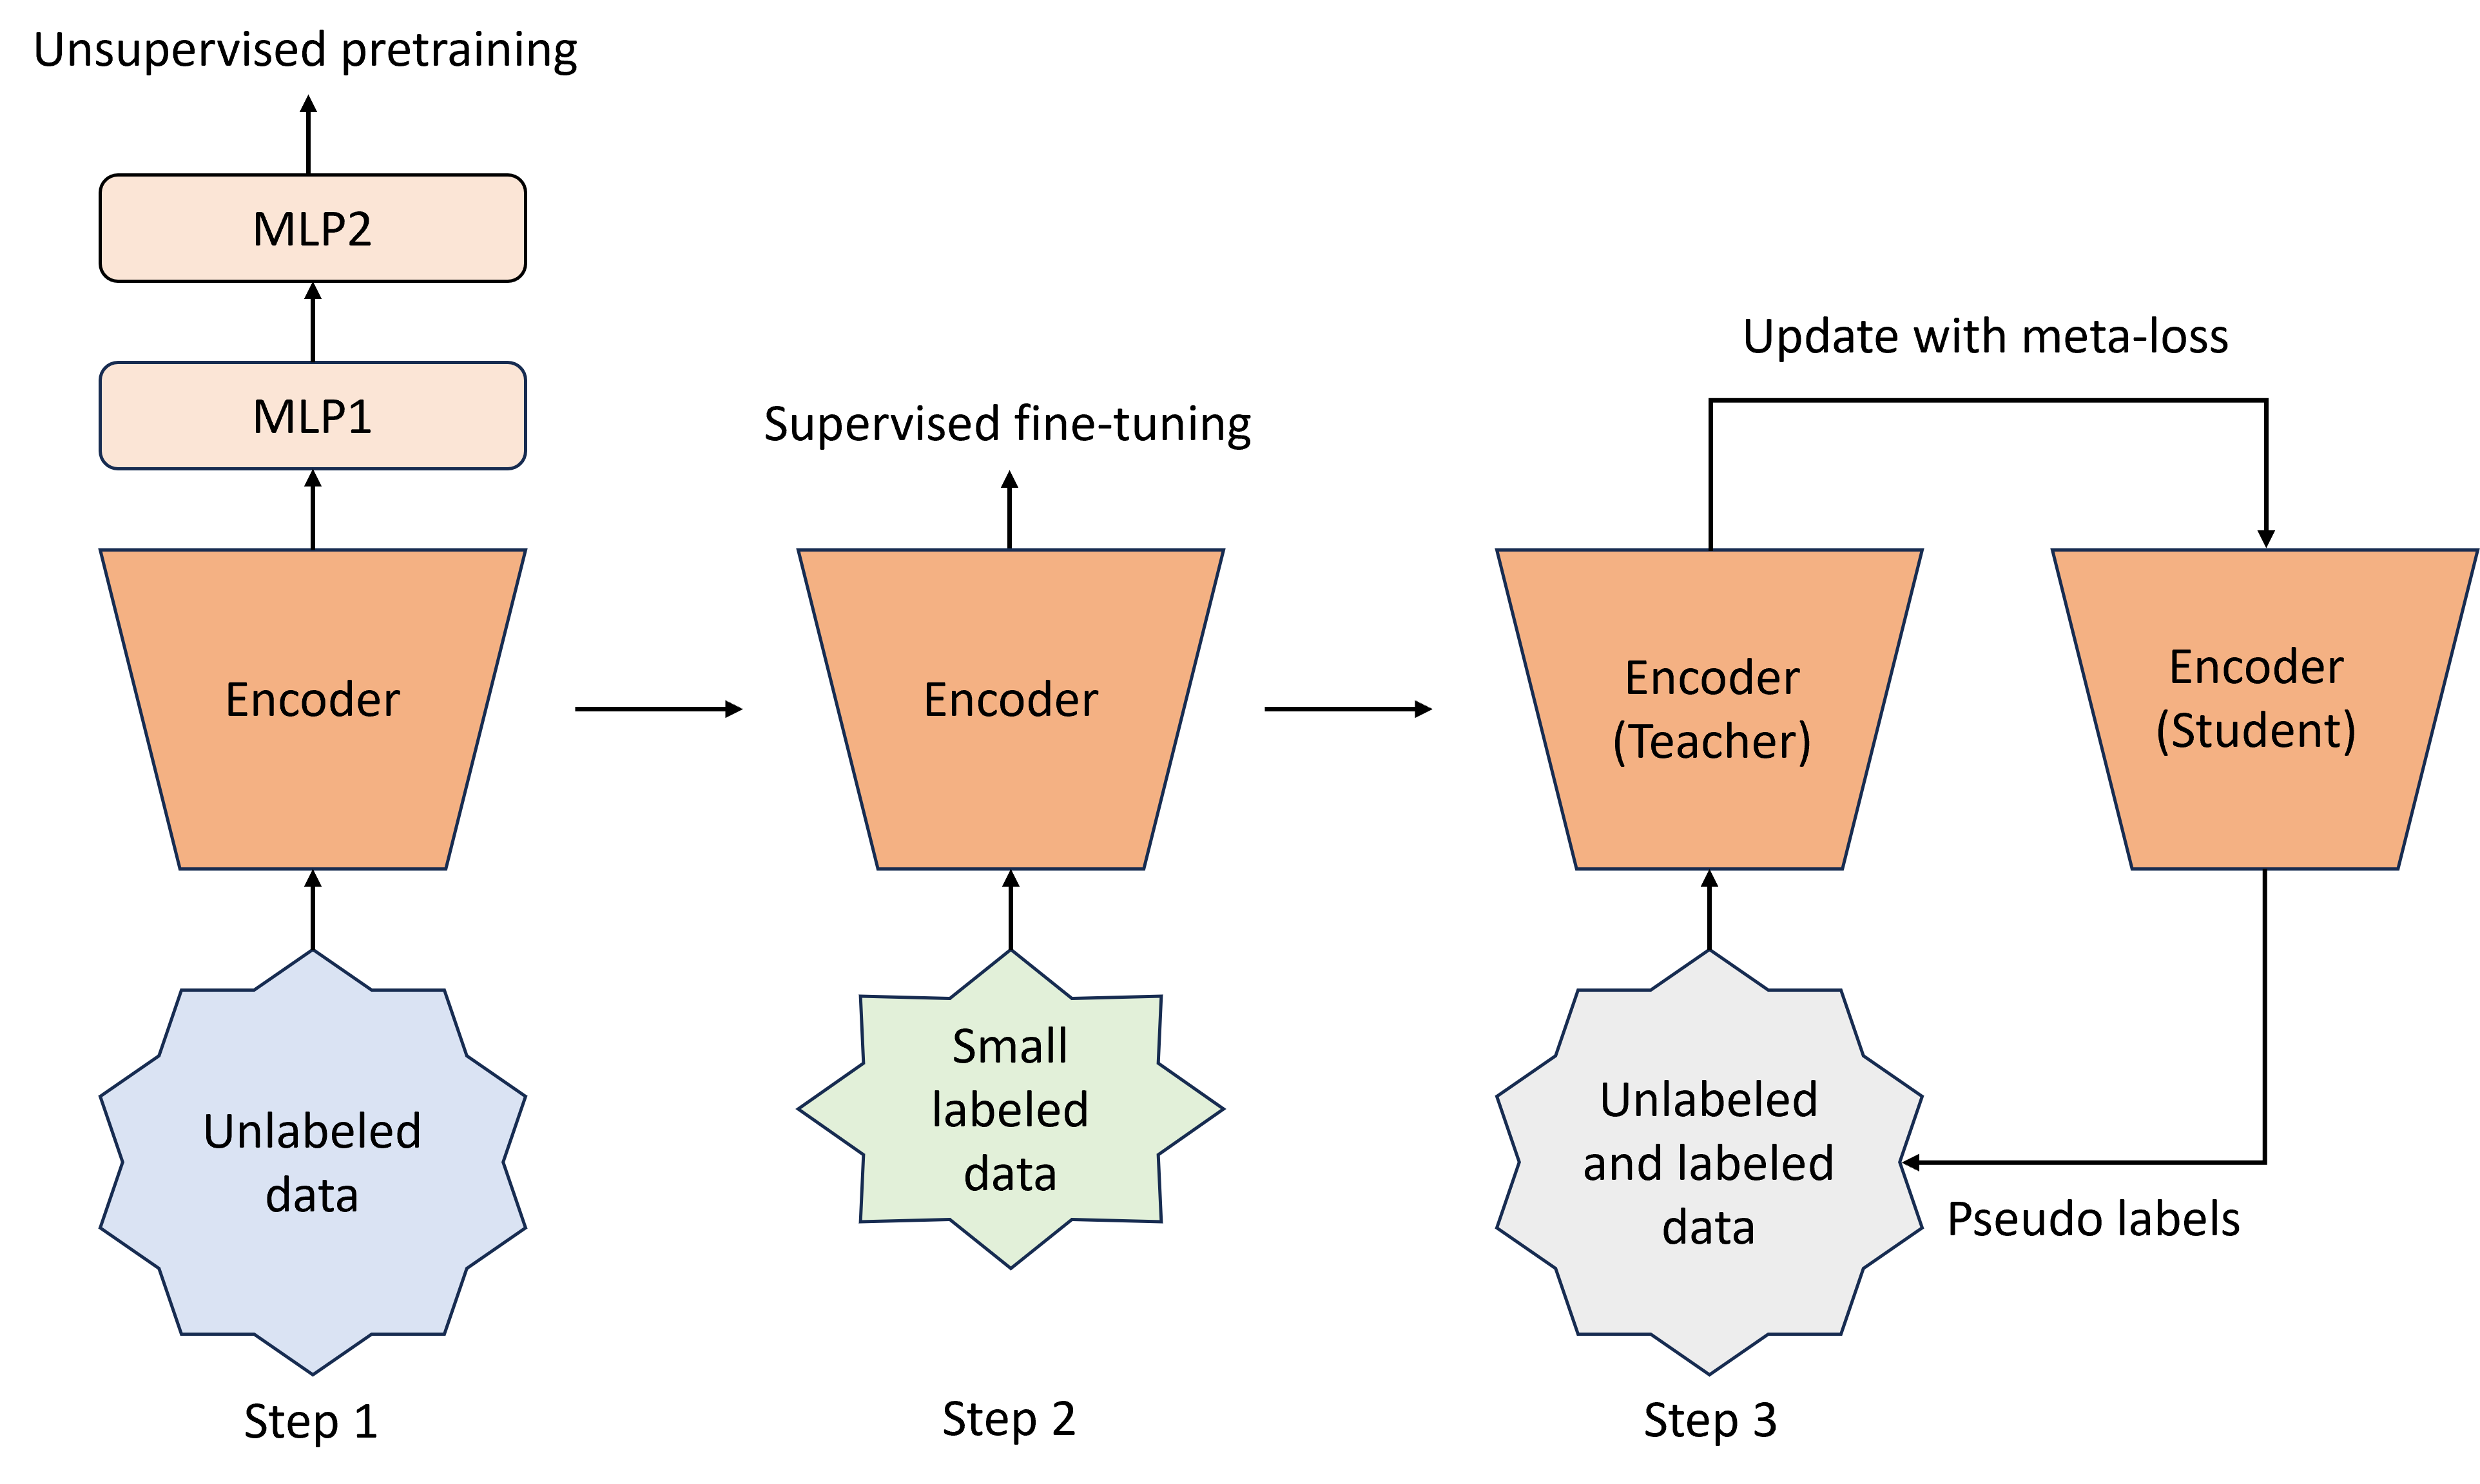
\includegraphics[width=0.9\textwidth]{FIGURES/rlpl/flow.png}
    \caption{\textbf{RLPL flowchart.} 
    RLPL has two levels of unlabeled data utilization. First, it employs unsupervised representation learning. Second, We obtain a highly accurate fine-tuned classifier using only a handful of label data. Lastly, through pseudo labelling using teacher-student networks, both initialized from superior supervised backbone, we improve the classifier further.}
    \label{fig:flow}
\end{figure*}
\section{Introduction}    

\subsection{Contributions}

In summary, our work contains the following contributions:

\begin{itemize}

    \item Our approach cleverly leverages most information from the inputs, leading to enhanced global representation learning. By making this strategic adjustment, our model achieves improved representations with a smaller batch size, ultimately achieving higher accuracy in the downstream tasks.
    
    \item During the downstream task, we utilize unlabeled samples a second time with pseudo labeling. Our approach uses the student network feedback with a meta-loss update to improve the noisy teacher \cite{xie2020self} as the final classifier.
    
    \item RLPL outperforms other State-Of-The-Art (SOTA) RL algorithms on an equivalent but more compact architecture, making it more efficient and cost-effective for edge computing in resource-constrained environments.
    
    \end{itemize}

\subsection{Proposed Methodology: RLPL}

We propose a novel framework, RLPL, effectively utilizes unlabeled data through two key innovations: (1) enhanced representation learning with auxiliary loss functions, and (2) refined pseudo-labeling with meta-learning. This section details the technical aspects of our approach.


\subsubsection{Improved Representation Learning}

In RLPL, the trainable and momentum networks use identical encoders for image embeddings. These embeddings are projected to a lower-dimensional space using a Multi-Layer Perceptron (MLP) in each network. The momentum network stops here, producing outputs with a dimension of 256. In contrast, the trainable network includes an additional prediction head, consisting of another MLP layer with the same dimension.

\begin{figure*}[!htbp]
    \centering
    % First subfigure
    \begin{subfigure}[b]{0.45\textwidth}
        \centering
        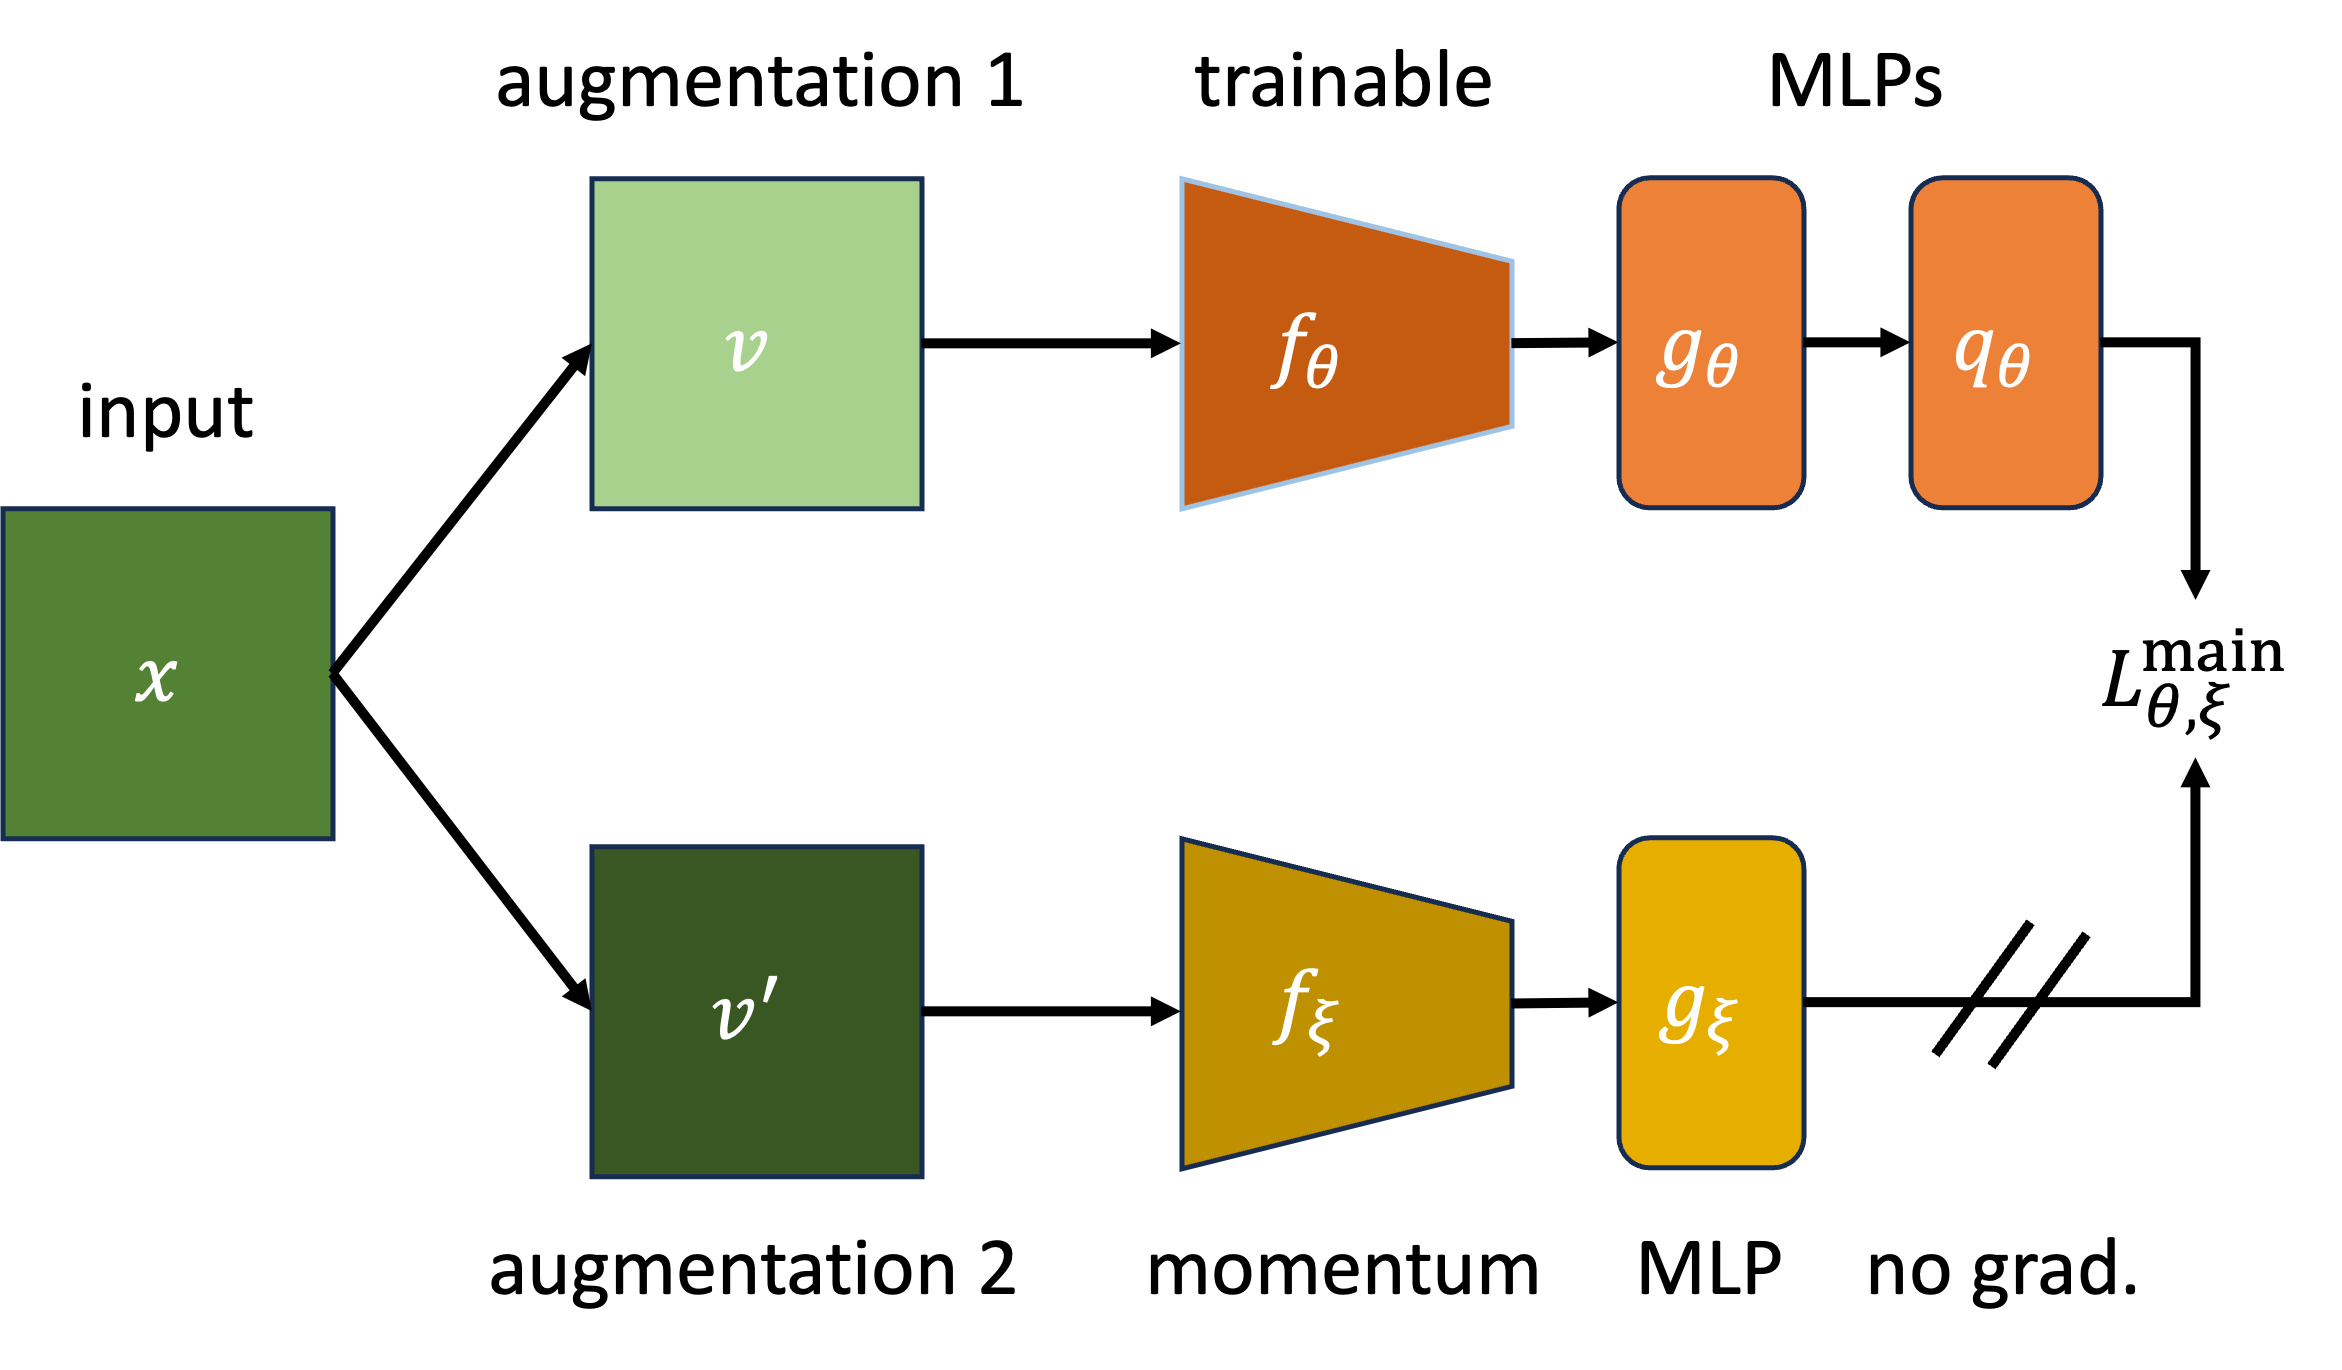
\includegraphics[width=\textwidth]{FIGURES/rlpl/rl1.png}
        \caption{main loss calculation}
        \label{fig:main loss}
    \end{subfigure}
    \hspace{0.02\textwidth} % Adjust space here
    % Second subfigure
    \begin{subfigure}[b]{0.45\textwidth}
        \centering
        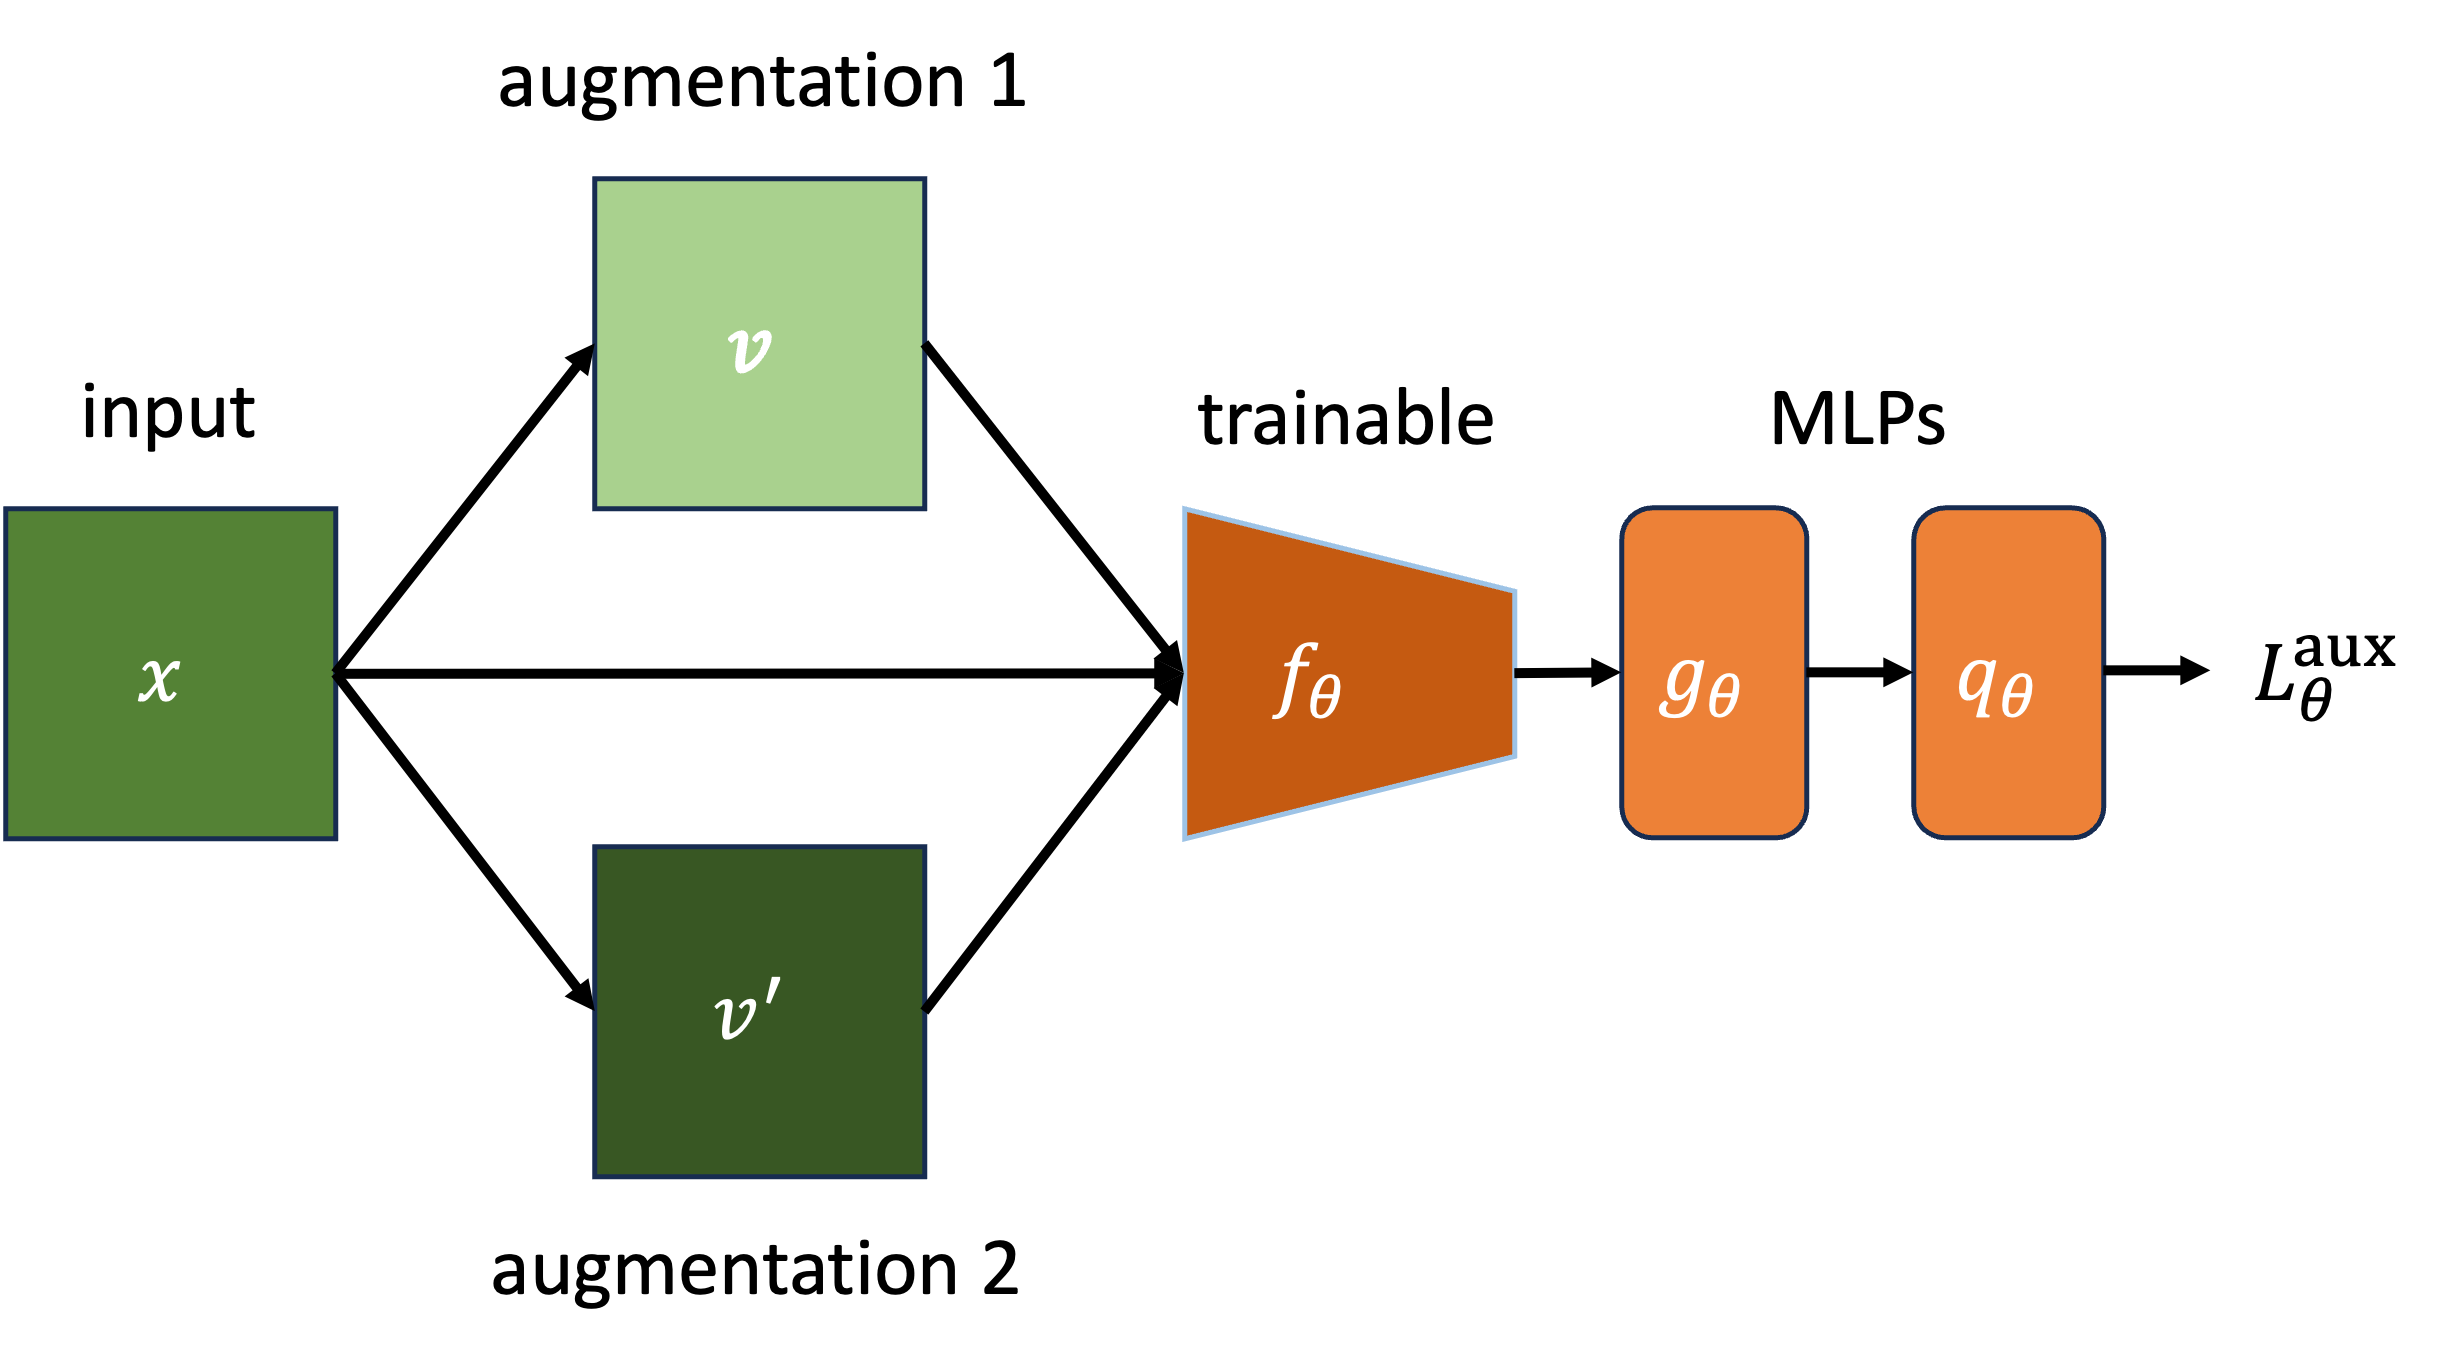
\includegraphics[width=\textwidth]{FIGURES/rlpl/rl2.png}
        \caption{auxiliary loss calculation}
        \label{fig:aux loss}
    \end{subfigure}
    
    \caption{Representation learning with RLPL: \textbf{(a)} The augmented inputs are processed through both networks to compute the main loss. \textbf{(b)} The original and augmented inputs are fed into the trainable network to compute the auxiliary loss.
    }

    \label{fig:two_photos}
\end{figure*}

RLPL learns a representation $y_{\theta}$ for downstream tasks using  encoder $f_{\theta}$, a projector $g_{\theta}$, and a predictor $q_{\theta}$. The momentum network, $f_{\xi}$, with a projector $g_{\xi}$, mirrors the trainable network's architecture but updates as an exponential moving average with decay rate, $\gamma \in [0,1]$:

\begin{equation}
\xi \leftarrow \gamma \xi + (1 - \gamma) \theta.
\end{equation}

For an input image $x$, we create two augmented views $v$ and ${v}'$. The trainable network computes $y_{\theta} \triangleq f_{\theta}(v)$ and $z_{\theta} \triangleq g_{\theta}(y_{\theta})$, while the momentum network outputs $y'_{\xi} \triangleq f_{\xi}(v')$ and $z'_{\xi} \triangleq g_{\xi}(y'_{\xi})$.

We then predict $z'_{\xi}$ from $z_{\theta}$ using $q_{\theta}(z_{\theta})$, and $l_2$-normalize both $q_{\theta}(z_{\theta})$ and $z'_{\xi}$ to $\bar{q}_{\theta}(z_{\theta}) \triangleq \frac{q_{\theta}(z_{\theta})}{\| q_{\theta}(z_{\theta}) \|_{2}}$ and $\bar{z}'_{\xi} \triangleq \frac{z'_{\xi}}{\| z'_{\xi} \|_{2}}$. The loss function is the mean squared error between the normalized prediction and momentum projection (as shown in Figure \ref{fig:main loss}):

\begin{equation} \label{eq:loss}
L_{\theta, \xi} \triangleq \left\| \bar{q}_{\theta}(z_{\theta}) - \bar{z}'_{\xi} \right\|_{2}^{2} = 2 - 2 \cdot \frac{\langle q_{\theta}(z_{\theta}), z'_{\xi} \rangle}{\| q_{\theta}(z_{\theta}) \|_{2} \cdot \| z'_{\xi} \|_{2}}.
\end{equation}

To symmetrize the loss, we feed $v'$ to the trainable network and $v$ to the momentum network, computing $\tilde{L}_{\theta, \xi}$. The combined loss for optimization is:

\begin{equation}
L_{\theta, \xi}^{\text{main}} = L_{\theta, \xi} + \tilde{L}_{\theta, \xi}.
\end{equation}

To calculate the auxiliary loss, the original image goes through the online network as an additional input (as shown in Figure \ref{fig:aux loss}). For original input $x$ and augmented views $v, v'$, we obtain outputs $q_{\theta}(z_{\theta }^{x})\triangleq q_{\theta}(g_{\theta}(f_{\theta}(x)))$, $q_{\theta}(z_{\theta }^{v})\triangleq q_{\theta}(g_{\theta}(f_{\theta}(v)))$, and $q_{\theta}(z_{\theta }^{v'})\triangleq q_{\theta}(g_{\theta}(f_{\theta}(v')))$, respectively. We design an auxiliary loss that allows gradient flow during backpropagation. This auxiliary loss is combined with the main loss, weighted by a factor \(\lambda\). The momentum network stays the same, but the trainable network affects its update parameters.

We calculate the mean of two output embeddings, $\bar{q_{\theta}}(z_{\theta }^{vv'})$, from the prediction head.

\begin{equation}
\bar{q_{\theta}}(z_{\theta }^{vv'}) =  \frac{1}{2}\left ( \bar{q_{\theta}}(z_{\theta}^{v}) + \bar{q_{\theta}}(z_{\theta}^{v'}) \right )
\end{equation}
where $\bar{q_{\theta}}(z_{\theta}^{v})$ and $\bar{q_{\theta}}(z_{\theta}^{v'})$ are the batch-mean of their respective embeddings, $q_{\theta}(z_{\theta}^{v})$ and $q_{\theta}(z_{\theta}^{v'})$.

Now, we denote the auxiliary loss as $L_{\theta}^{\text{aux}}$ and it is expressed as,
\begin{equation}
L_{\theta}^{\text{aux}} = \left \| \bar{q_{\theta}}(z_{\theta}^{x}) - \bar{q_{\theta}}(z_{\theta}^{vv'})\right \|_{2}^{2}
\end{equation}

where $\bar{q_{\theta}}(z_{\theta}^{x})$ is the batch-mean of ${q_{\theta}}(z_{\theta}^{x})$.

% \begin{equation}
% \text{mean}(\bar{q_{\Theta}^{v}}(z_{\Theta}), \bar{q_{\Theta}^{v'}}(z_{\Theta})) = \frac{\bar{q_{\Theta}^{v}}(z_{\Theta}) + \bar{q_{\Theta}^{v'}}(z_{\Theta})}{2}.
% \end{equation}

Next, it is added to the main loss with a weight, $\lambda$, to obtain the total loss.

\begin{equation}
L_{\theta, \xi} = L_{\theta, \xi}^{\text{main}} + \lambda L_{\theta}^{\text{aux}}
\end{equation}

% \noindent where $\lambda$ is the weight for the auxiliary loss.

Optimization updates the trainable network parameters $\theta$ with a learning rate $\eta$, while the momentum network parameters are updated as follows:

\begin{equation}
\theta \leftarrow \text{optimizer}(\theta, \nabla_{\theta} L_{\theta, \xi}, \eta),
\end{equation}

\begin{equation}
\xi \leftarrow \gamma \xi + (1 - \gamma) \theta.
\end{equation}

After training, only the encoder $f_{\theta}$ is returned for the downstream tasks. The pseudo-code for these steps is provided in Algorithm \ref{alg:bywl}.

% \begin{figure}[t]
\begin{algorithm}[!htbp]
\caption{Representation learning with RLPL} \label{alg:bywl}
\begin{algorithmic}
\State \textcolor{pythoncomment}{\# f\_t: trainable net (backbone + projector + predictor)}
\State \textcolor{pythoncomment}{\# f\_m: momentum net (backbone + projector)}
\State \textcolor{pythoncomment}{\# lambda: weight of auxiliary loss}
\State \textcolor{pythoncomment}{\# gma: momentum update rate}

\State \text{}
\State  \textcolor{pythonfunction}{for} x \textcolor{pythonfunction}{in} loader: \textcolor{pythoncomment}{\# load a minibatch}
\State \hspace{1.1em} v1, v2 = augment(x) \textcolor{pythoncomment}{\# two random augmentations}

\State \text{}

\State \hspace{1.1em} \textcolor{pythoncomment}{\# compute embeddings}
\State \hspace{1.1em}	t, t1, t2 = f\_t(x), f\_t(v1), f\_t(v2)  , \textcolor{pythoncomment}{\# $N \times D$}

\State \text{}

\State \hspace{1.1em}	\textcolor{purpleish}{with} torch.no\_grad(): \textcolor{pythoncomment}{\# stop the gradient}
\State \hspace{2.5em}	m1, m2 = f\_m(v1), f\_m(v2) \textcolor{pythoncomment} {\# $N \times D$}

\State \text{}

\State \hspace{1.1em} \textcolor{pythoncomment}{\# calculate the losses}
\State \hspace{1.1em}	loss\_main = (loss1(t1, m2) + loss1(t2, m1)).mean()
\State \hspace{1.1em} loss\_aux = loss2(t, t1, t2)
\State \hspace{1.1em}	total\_loss = loss\_main + lambda * loss\_aux
\State \hspace{1.1em} total\_loss.backward() \textcolor{pythoncomment}{\# optimization step}
\State \hspace{1.1em} update(f\_t.params)

\State \text{}

\State \hspace{1.1em} \textcolor{pythoncomment}{\# momentum network update}
\State \hspace{1.1em} f\_m.params = gma*f\_m.params+(1-gma)*f\_t.params

\State \text{}

\State \textcolor{pythonfunction}{def} loss1(a, b):  \textcolor{pythoncomment}{\# main loss function}
\State \hspace{1.1em} a = normalize(a, dim=-1)
\State \hspace{1.1em} b = normalize(b, dim=-1)
\State \hspace{1.1em} loss = 2 - 2 * (a * b).\textcolor{pythonfunction}{sum}(dim=-1) 
\State \hspace{1.1em} \textcolor{pythonfunction}{return} loss.mean()

\State \text{}

\State \textcolor{pythonfunction}{def} loss2(a, b, c): \textcolor{pythoncomment}{\# auxiliary loss function}
\State \hspace{1.1em}	avr\_emb = mean(b, c, dim=-1)
\State \hspace{1.1em} loss = loss1(a - avr\_emb)
\State \hspace{1.1em} \textcolor{pythonfunction}{return} loss.mean()
\end{algorithmic}
\end{algorithm}
% \end{figure}

\subsubsection{Effective Pseudo Labeling}  

For effective pseudo-labeling, let, $f_{\theta_T}$ and $f_{\theta_S}$ denote teacher and student networks initialized with parameters $\theta_T, \theta_S \leftarrow \theta$ from the pretrained encoder. Given a batch of labeled samples $(x_l, y_l) \in \mathcal{D}_l$ and unlabeled samples $x_u \in \mathcal{D}_u$, we formulate an iterative pseudo-labeling framework.

For each iteration, we first compute the student's initial loss on labeled data:

\begin{equation}
L_{s1} = \mathbb{E}_{(x_l,y_l)\sim\mathcal{D}_l}[\text{CE}(f_{\theta_S}(x_l), y_l)]
\end{equation}

For unlabeled data $x_u$, the teacher network generates soft pseudo-labels through weak augmentation $\mathcal{A}$:

\begin{equation}
\hat{y}_u = f_{\theta_T}(\mathcal{A}(x_u))
\end{equation}

To ensure quality of pseudo-labels, we filter predictions based on confidence threshold $\tau$:

\begin{equation}
\mathcal{M}_u = \{(x_u, \hat{y}_u) | \max(f_{\theta_T}(\mathcal{A}(x_u))) \geq \tau\}
\end{equation}

The teacher then learns from the filtered pseudo-labeled data:

\begin{equation}
L_u = \mathbb{E}_{(x_u,\hat{y}_u)\sim\mathcal{M}_u}[\text{CE}(f_{\theta_T}(x_u), \hat{y}_u)]
\end{equation}

After updating the student parameters using $L_u$, we measure its new performance:

\begin{equation}
L_{s2} = \mathbb{E}_{(x_l,y_l)\sim\mathcal{D}_l}[\text{CE}(f_{\theta_S}(x_l), y_l)]
\end{equation}

The effectiveness of pseudo-labeling is captured by the performance change:

\begin{equation}
\Delta L_s = L_{s2} - L_{s1}
\end{equation}

We incorporate this feedback through a meta-loss:

\begin{equation}
L_{\text{meta}} = \Delta L_s \cdot L_u
\end{equation}

The final objective for updating the teacher combines supervised learning on labeled data with the meta-loss feedback:

\begin{equation}
L_{\text{total}} = \underbrace{\mathbb{E}_{(x_l,y_l)\sim\mathcal{D}_l}[\text{CE}(f_{\theta_T}(x_l), y_l)]}_{\text{supervised loss}} + \underbrace{L_{\text{meta}}}_{\text{feedback}}
\end{equation}

This formulation creates a feedback loop where the teacher's pseudo-labeling strategy is dynamically adjusted based on the student's learning outcomes. When $\Delta L_s < 0$, indicating improved student performance, the teacher is encouraged to maintain its current strategy. Conversely, when $\Delta L_s > 0$, suggesting degraded performance, the teacher receives a stronger gradient signal to modify its approach.

The optimization proceeds iteratively:

\begin{align}
\theta_S &\leftarrow \theta_S - \eta_S \nabla_{\theta_S} L_u \\
\theta_T &\leftarrow \theta_T - \eta_T \nabla_{\theta_T} L_{\text{total}}
\end{align}

where $\eta_S$ and $\eta_T$ are learning rates for student and teacher networks respectively. After training convergence, only the teacher network is retained for deployment. The pseudo-code is provided in Algorithm~\ref{alg:PL}.

\begin{algorithm}[!htbp]
\caption{Pseudo labeling with RLPL} \label{alg:PL}
\begin{algorithmic}

\State \textcolor{pythoncomment}{\# f\_t: pretrained encoder}
\State \textcolor{pythoncomment}{\# n\_t, n\_s: teacher and student networks}
\State \textcolor{pythoncomment}{\# tau: pseudo labels threshold}

\State \text{}

% \State \textcolor{pythoncomment}{\# initialize teacher and student networks}

\State n\_t = f\_t.state\_dict() \textcolor{pythoncomment}{\# initialize teacher}
\State n\_s = f\_t.state\_dict() \textcolor{pythoncomment}{\# initialize student}

\State \text{}

\State \textcolor{pythoncomment}{\# load a minibatch of labeled and unlabeled samples}
\State  \textcolor{pythonfunction}{for} x, y, x\_u \textcolor{pythonfunction}{in} loader:
\State \hspace{1.1em}	\textcolor{purpleish}{with} torch.no\_grad(): \textcolor{pythoncomment}{\# stop the gradient}
\State \hspace{2.5em} loss\_s1 = cross\_entropy(n\_s(x), y)
\State \hspace{1.1em} y\_u = n\_t(x\_u) 

\State \text{}

\State \hspace{1.1em} \textcolor{pythoncomment}{\# filtering unlabled samples based on threshold}
\State \hspace{1.1em} x\_u, y\_u = x\_u $\left[  \text{y\_u} \geq \text{tau}\right]$, y\_u $\left[  \text{y\_u} \geq \text{tau}\right]$
\State \hspace{1.1em} y\_ut = n\_t(augment(x\_u))  \textcolor{pythoncomment}{\# weak augmentation}
\State \hspace{1.1em} loss\_t = cross\_entropy(y\_ut, y\_u)
\State \hspace{1.1em} loss\_t.backward()
\State \hspace{1.1em} update(n\_s.params) \textcolor{pythoncomment}{\# student network update}

\State \text{}

\State \hspace{1.1em}	\textcolor{purpleish}{with} torch.no\_grad(): \textcolor{pythoncomment}{\# stop the gradient}
\State \hspace{2.5em} loss\_s2 = cross\_entropy(n\_s(x), y)
\State \hspace{1.1em} change = loss\_s2 - loss\_s1
\State \hspace{1.1em} meta\_loss = change * loss\_t \textcolor{pythoncomment}{\# meta-loss computation}
\State \hspace{1.1em} loss = cross\_entropy(n\_t(x), y)
\State \hspace{1.1em} total\_loss = loss + meta\_loss \textcolor{pythoncomment}{\# total loss}
\State \hspace{1.1em} total\_loss.backward()
\State \hspace{1.1em} update(n\_t.params) \textcolor{pythoncomment}{\# teacher network update}

\end{algorithmic}
\end{algorithm}

\subsection{Experiments}

We conduct extensive experiments to evaluate RLPL's performance across multiple datasets and settings. Our analysis focuses on three key aspects: (1) the effect of batch size on representation learning quality, (2) comparison with state-of-the-art methods on standard benchmarks, and (3) ablation studies to validate our design choices. The following sections detail our experimental setup and findings.

\subsubsection{Datasets}

% In our experiments, we applied STL-10 \cite{singh2019justification}, CIFAR-10 \cite{ho2018cifar10} and SVHN \cite{sermanet2012convolutional} datasets for unlabeled RL training. The STL-10 dataset is specially designed for unsupervised feature learning as it contains $13,000$ labeled images across $10$ classes and $100,000$ unlabeled images. While we used the entire training set of CIFAR-10 and SVHN datasets for RL, we only used $250$, $1,000$, and $4,000$ labeled training samples in downstream classifications. Additional experiments were conducted on 6 other image datasets \cite{krizhevsky2009learning, xiao2017fashionmnist, LFWTech, helber2019eurosat, nilsback2008automated, imagenette2019} with different class numbers.

Our experiments utilized a diverse collection of image datasets to thoroughly evaluate the effectiveness of our proposed approach. Below, we provide a detailed description of each dataset used in our study:

\noindent \textbf{STL-10} \cite{singh2019justification} is specifically designed for unsupervised and self-supervised learning research. It contains 13,000 labeled images across 10 object categories (airplane, bird, car, cat, deer, dog, horse, monkey, ship, and truck) and 100,000 unlabeled images sampled from a similar but broader distribution. A key characteristic of STL-10 is its relatively high-resolution images (96×96 pixels), making it more challenging than lower-resolution alternatives. The limited labeled training set (500 images per class) combined with abundant unlabeled data makes it an ideal benchmark for semi-supervised learning approaches, closely mirroring real-world scenarios where labeled data is scarce.

\noindent \textbf{CIFAR-10} \cite{ho2018cifar10} consists of 60,000 color images (32×32 pixels) divided into 10 mutually exclusive classes (airplane, automobile, bird, cat, deer, dog, frog, horse, ship, truck). The dataset is split into 50,000 training and 10,000 test images, with each class having an equal number of samples. While the entire training set was used for representation learning, we specifically created label-limited scenarios with only 250, 1,000, and 4,000 labeled examples to evaluate model performance under varying degrees of supervision. This approach allows us to assess how effectively our method leverages unlabeled data when labeled samples are extremely scarce.

\noindent \textbf{SVHN} \cite{sermanet2012convolutional} (Street View House Numbers) is derived from Google Street View images and presents a real-world object recognition task focused on digit classification. It contains over 600,000 digit images in its complete version, with 73,257 digits for training, 26,032 for testing, and an additional 531,131 less difficult samples that can be used as extra training data. Unlike handwritten digit datasets, SVHN presents additional challenges with real-world variations in lighting, orientation, and background clutter. The images are 32×32 pixels in color, and like CIFAR-10, we constructed supervision-limited scenarios with 250, 1,000, and 4,000 labeled examples.

For transfer learning evaluation, we employed six additional image datasets with varying characteristics:

\noindent \textbf{CIFAR-100} \cite{krizhevsky2009learning} is similar to CIFAR-10 in image size (32×32 pixels) but contains 100 fine-grained classes grouped into 20 superclasses. With 600 images per class (500 training, 100 testing), it presents a more challenging fine-grained classification task.

\noindent \textbf{Fashion-MNIST} \cite{xiao2017fashionmnist} is designed as a more challenging drop-in replacement for the traditional MNIST dataset. It consists of 70,000 grayscale images (28×28 pixels) of fashion items across 10 categories, divided into 60,000 training and 10,000 test examples. This dataset helps evaluate model performance on grayscale images with more complex patterns than digits.

\noindent \textbf{LFW} \cite{LFWTech} (Labeled Faces in the Wild) contains 13,233 face images of 5,749 individuals collected from the web. These images present natural variations in pose, lighting, expression, and background, making it a challenging benchmark for face recognition tasks. We used the aligned version of the dataset with cropped faces.

\noindent \textbf{EuroSAT} \cite{helber2019eurosat} is a land use and land cover classification dataset derived from Sentinel-2 satellite imagery. It contains 27,000 labeled images (64×64 pixels) across 10 classes, representing various land use patterns. This dataset helps evaluate the model's performance on remote sensing applications.

\noindent \textbf{Oxford Flowers 102} \cite{nilsback2008automated} includes 8,189 images of 102 flower categories common in the United Kingdom. Each class contains between 40-258 images with significant variations in scale, pose, and lighting. This fine-grained classification task presents a different challenge due to its natural image variability and smaller sample size per class.

\noindent \textbf{Imagenette} \cite{imagenette2019} is a subset of 10 easily distinguishable classes from ImageNet (tench, English springer, cassette player, chain saw, church, French horn, garbage truck, gas pump, golf ball, parachute). With approximately 13,000 training images and larger dimensions than the other datasets, it tests the model's ability to handle higher-resolution natural images.

This diverse collection of datasets enables a comprehensive evaluation of our proposed method across a wide range of image domains, resolutions, class numbers, and task difficulties, demonstrating its versatility and general applicability to various computer vision scenarios.


\subsubsection{Implementation Details} 

\textbf{Image augmentations:} Our augmentation pipeline follows SimCLR and BYOL, using PyTorch~\cite{paszke2019pytorch}. We apply "RandomResizedCrop" (scale: [0.2, 1.0]), "RandomHorizontalFlip", "ColorJitter" (brightness, contrast, saturation: 0.4, hue: 0.1), "RandomGrayscale" (p=0.2), and "GaussianBlur" ($\sigma$=[1.0, 2.0], p=0.2). Images are normalized using standard mean and variance values. 

Our experiments reveal that image resolution significantly affects accuracy; thus, we resize all images to \(256 \times 256\). In the PL phase, weak augmentations are applied to the teacher model, involving random horizontal and vertical flips, each with a probability of \(0.25\).

\noindent
\textbf{Architecture:} We use ResNet18 \cite{ayyachamy2019medical}, a more computationally feasible network, designed for GPU computations. This ResNet18 architecture remains consistent across all settings, including representation learning, and pseudo labeling. The MLPs, projection, and prediction layers adhere to the parameters established by BYOL. In PL, the teacher and student networks are initialized from the ResNet18, pre-trained via RL.

\noindent
\textbf{Optimization:} The RL framework was optimized using the Adam optimizer \cite{zhang2018improved}, whereas PL employed the Stochastic Gradient Descent (SGD) optimizer \cite{gower2019sgd}, both with a learning rate set to $0.0003$. The auxiliary loss is weighted at \(0.5\). RL underwent training for $50$ epochs with a batch size of $128$, while PL was trained over $150$ epochs with a batch size of $16$.

\begin{figure}[!htbp]
    \centering
    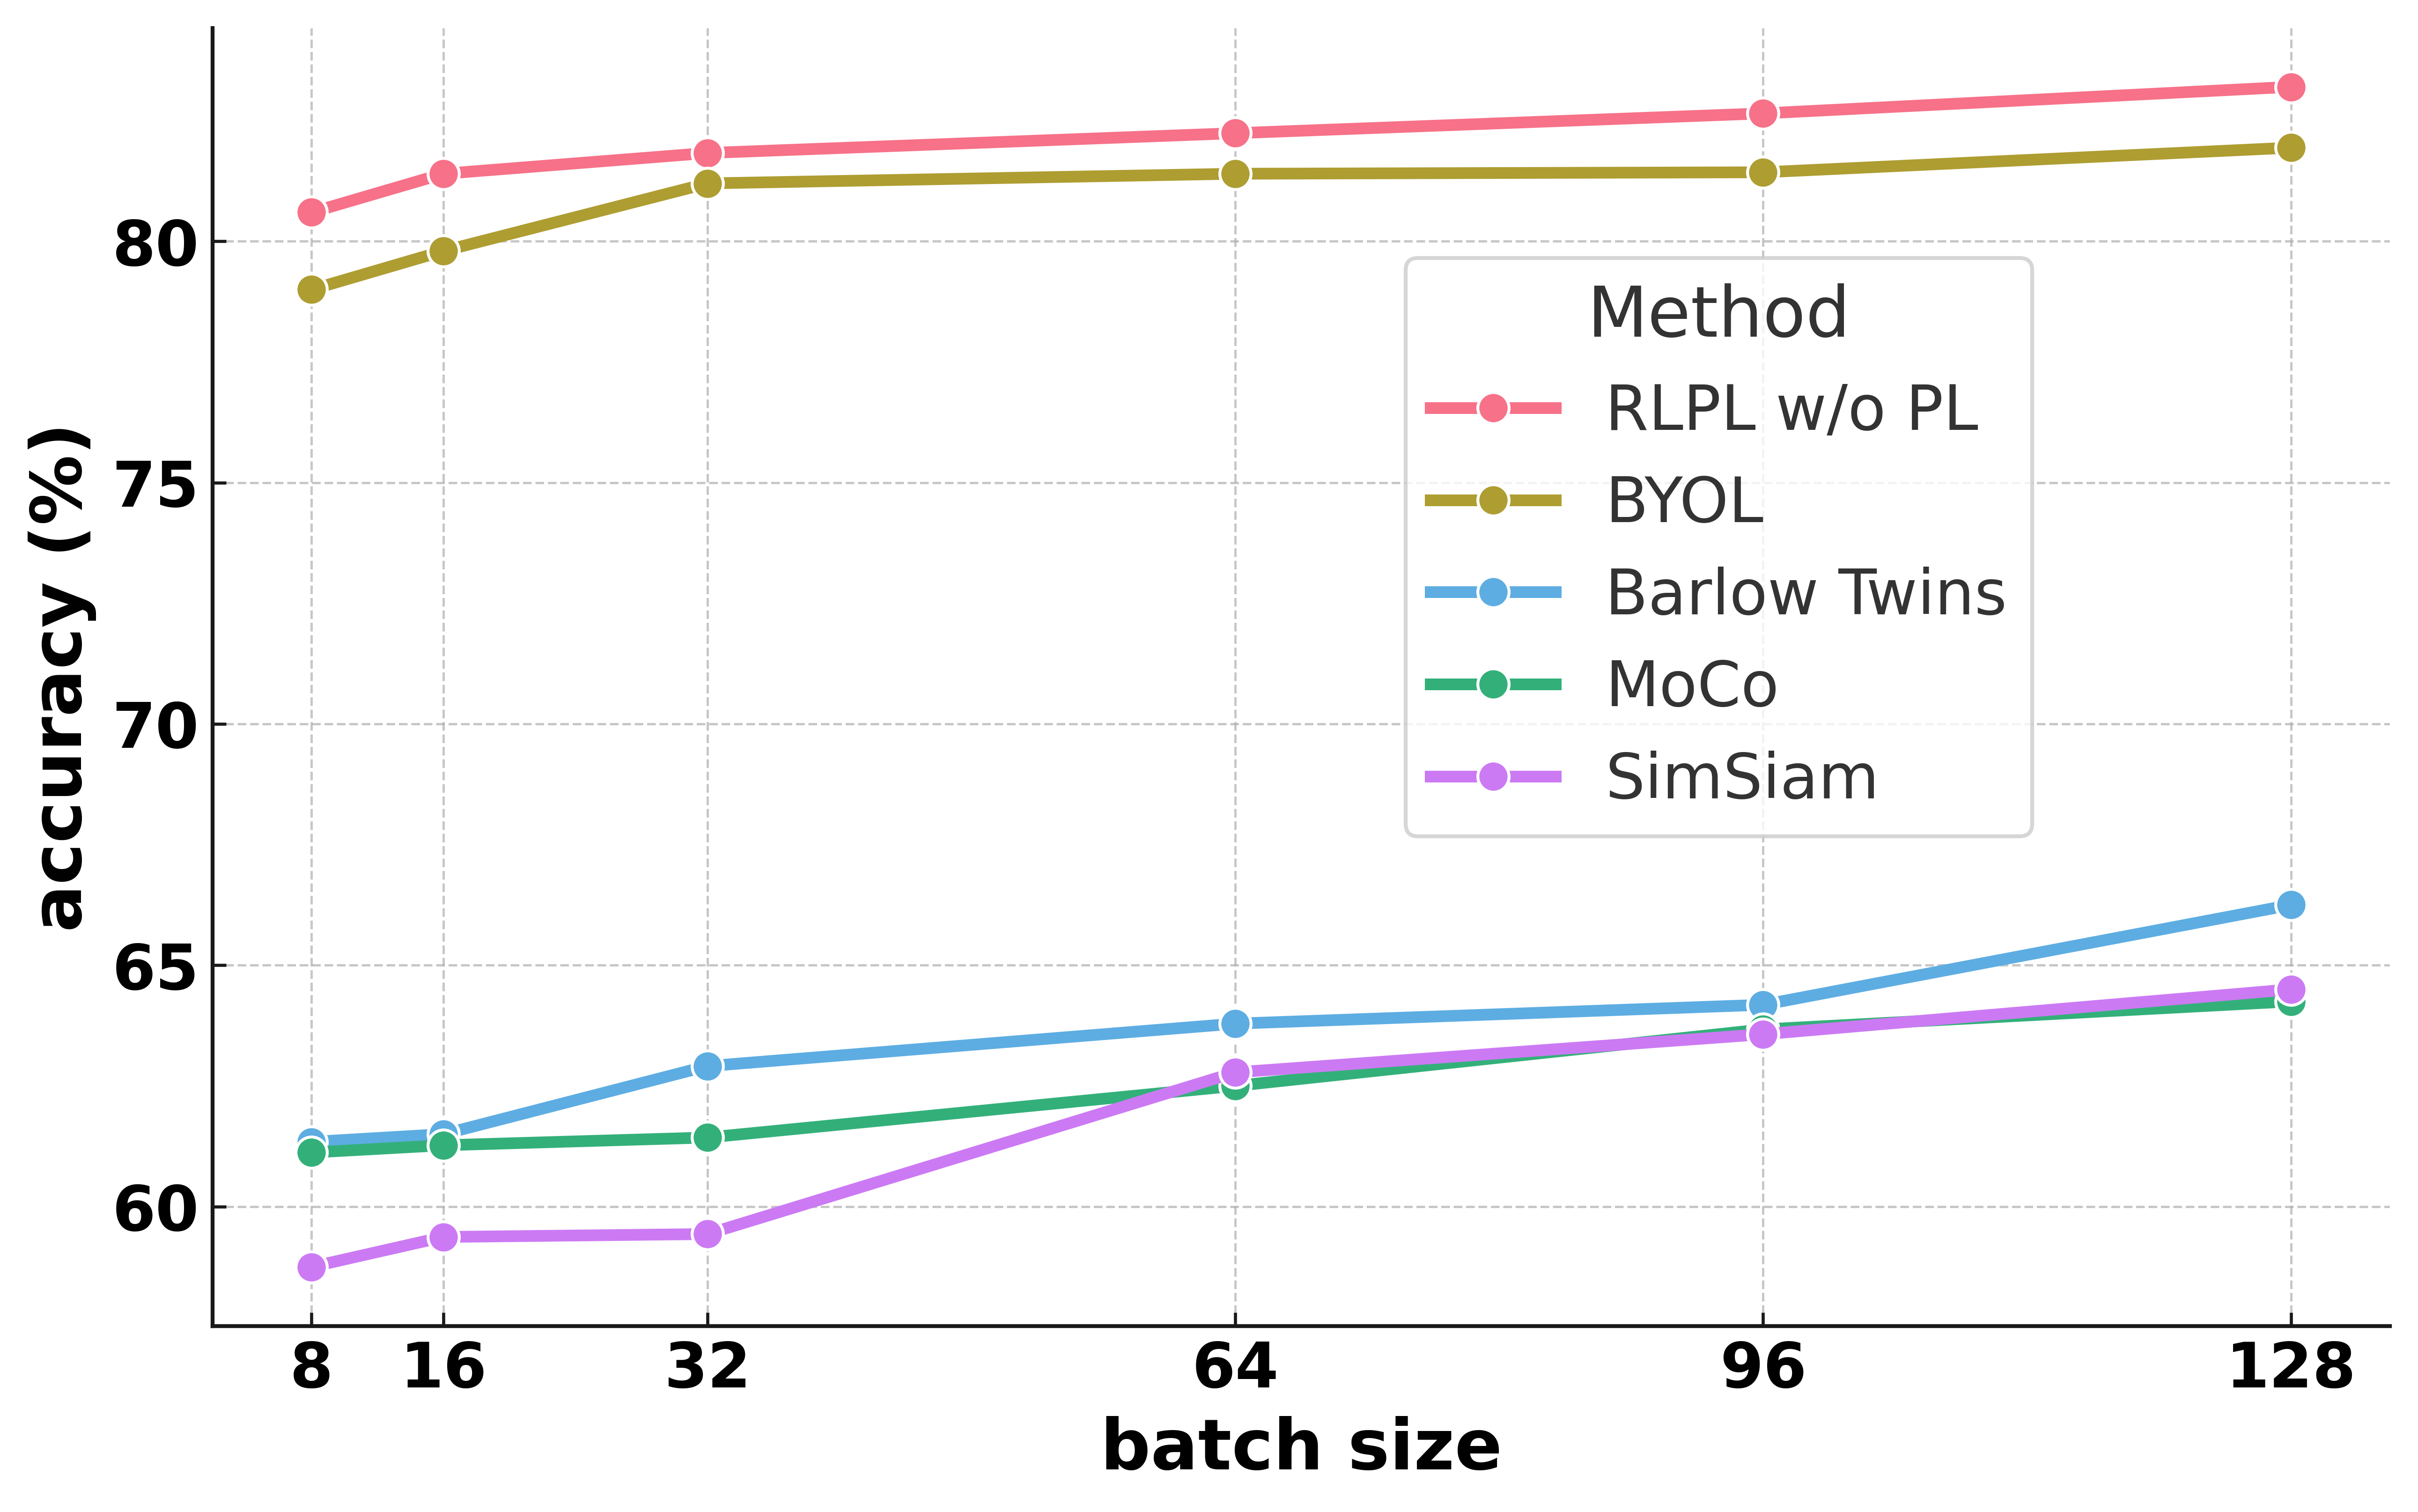
\includegraphics[width=0.9\columnwidth, keepaspectratio]{FIGURES/rlpl/accuracy_vs_batch.png}
    \caption{Effect of batch size on model performance (evaluated on STL-10).}
    \label{fig:batch}
\end{figure}

\begin{table}[htbp]
    \centering
    \begin{tabular}{l c}
      \toprule
      \textbf{Methods} & \textbf{Test Accuracy (\%)} \\  
      \midrule
      Baseline (ResNet18) & 53.16 \\
      FixMatch \cite{sohn2020fixmatch} & 37.28 \\ 
      MixMatch \cite{berthelot2019mixmatch} & 71.60 \\
      MoCo & 66.25 \\
      SimSiam & 64.50 \\
      Barlow Twins & 64.25 \\
      BYOL & 81.94  \\
      RLPL (Ours) & \textbf{84.64} \\
      \bottomrule
    \end{tabular}
    \caption{Performance of different methods on STL-10 dataset.}
    \label{table:stl}
\end{table}

\subsection{Results and Discussion}

\begin{table}[htbp]
    \centering
    \resizebox{\textwidth}{!}{%
    \begin{tabular}{llllllll}
    \hline
    \multirow{2}{*}{\bf Method} & \multicolumn{3}{c}{\bf CIFAR-10} & \multicolumn{3}{c}{\bf SVHN} & \multirow{2}{*}{\bf Average} \\ 
    \cmidrule(lr){2-4} \cmidrule(lr){5-7}
     & \bf 250 labels & \bf 1000 labels & \bf 4000 labels & \bf 250 labels & \bf 1000 labels & \bf 4000 labels & \\ \hline
    ResNet18 & 33.90 & 43.71 & 58.47 & 41.20 & 84.58 & 87.60 & 58.24 \\
    MoCO     & 34.50 & 46.75 & 61.88 & 30.75 & 83.25 & 89.12 & 57.37 \\
    SimSiam  & 23.88 & 29.50 & 48.88 & 14.62 & 51.25 & 67.38 & 39.92 \\
    Barlow Twins & 35.88 & 47.75 & 63.75 & 21.88 & 79.01 & 88.25 & 56.42 \\
    BYOL     & 33.19 & 46.92 & 59.29 & 67.00 & 85.60 & 88.20 & 63.70 \\
    RLPL (ours) & \bf 48.93 & \bf 52.45 & \bf 65.69 & \bf 72.12 & \bf 88.39 & \bf 92.78 & \bf 70.39 \\ \hline
    \end{tabular}%
    }
    \caption{Test accuracy (\%) of different methods on varying numbers of training samples.}
    \label{table:2}
\end{table}


\begin{table}[!htbp]
\centering
\resizebox{\textwidth}{!}{
\begin{tabular}{lllllllll}
\hline
\multirow{2}{*}{\bf Method} & \multirow{2}{*}{\bf STL-10} & \multicolumn{3}{c}{\bf CIFAR-10}           & \multicolumn{3}{c}{\bf SVHN} & \multirow{2}{*}{\bf Average} \\ \cmidrule(lr){3-5}\cmidrule(lr){6-8}
                 &       & \bf 250 labels & \bf 1000 labels & \bf 4000 labels & \bf 250 labels & \bf 1000 labels & \bf 4000 labels & \\ \hline
PL (random init.)      &     53.34         &    30.49        &     40.57        &   55.90         &        11.19    &      17.62       &    75.62       &   40.39 \\
RLPL w/o PL      &      83.20        &    34.54       &     48.48        &   59.60          &     71.25      &       85.54      &     89.00      &   67.66 \\
RLPL (ours)    &    \bf 84.64       & \bf  48.93        &   \bf     52.45     &  \bf     65.69      & \bf    72.12       &    \bf   88.39     &  \bf   92.78  & \bf 72.14 \\ \hline
\end{tabular}
}
\captionof{table}{Test accuracy (\%) for ablation on methods.}
\label{table:ablation}
\end{table}


Our evaluation methods primarily comprise the baseline model, BYOL, SimSiam, MoCo, Barlaw Twins, RLPL, and two additional semi-supervised algorithms, FixMatch \cite{sohn2020fixmatch}, and MixMatch \cite{berthelot2019mixmatch} on the considered datasets. In all our experiments, we re-implemented each algorithm on a ResNet18 backbone with identical hyperparameters to ensure a fair comparison.

\subsubsection{Effect of Batch Size}

To illustrate the effectiveness of RLPL with reduced batch sizes, we present the results in Figure \ref{fig:batch}. We started with a batch size of $8$ for RLPL. Subsequently, we gradually increased the batch sizes for RLPL and others to evaluate their performances. To have a fair comparison, we applied the classification tasks only on the learned representation of RL, without any use of PL. As anticipated, the accuracy diminished with smaller batch sizes. Remarkably, at a batch size of $64$, RLPL attained an accuracy of $82.24\%$, surpassing BYOL's accuracy of $81.94\%$ with a batch size of $128$. All other methods, including Barlow Twins, MoCo, and SimSiam, achieve significantly lower accuracy in the small-scale implementation, with their performance further declining as batch size decreases. Although all methods exhibited a decline in accuracy with further reductions in batch sizes, RLPL consistently outperformed BYOL and all the others.

\subsubsection{Classification Accuracy}

Table \ref{table:stl} reports the classification accuracy on the STL-10 dataset. The ResNet18 classifier demonstrates challenges in reaching acceptable accuracy levels. For a fair comparison, all methods, including FixMatch and MixMatch, were implemented with a ResNet18 backbone and an identical batch size.

The results reveal that FixMatch struggles to achieve competitive accuracy, likely due to the limitations of pseudo-labeling techniques, which often require robust initialization and a deep backbone to perform effectively. While MixMatch shows considerable improvement, it still falls short of the performance attained by BYOL and RLPL. MoCo, SimSiam, and Barlow Twins achieve almost similar but lower accuracy. Notably, BYOL achieves an accuracy of $81.94\%$, whereas RLPL surpasses this with an accuracy of $84.64\%$, obtaining a $\textbf{2.7\%}$ improvement over BYOL.

Table \ref{table:2} compares ResNet18, the four primary methods central to this study, and RLPL across varying training samples. For both datasets, all methods showed progressively higher accuracies with increasing sample sizes. We observe that our method uniquely achieves acceptable accuracy on CIFAR-10 with only 250 labels, whereas other methods struggle under the same conditions. For SVHN with 250 labels, only BYOL and RLPL reach satisfactory accuracy, while other methods perform notably worse. Notably, Notably, RLPL consistently achieved the highest accuracy across all datasets and under all varying configurations, outperforming other methods in each case.

We include a column displaying the average test accuracy across all setups to provide a comprehensive view of the relative performance of each method. Only BYOL comes close to RLPL's performance; however, it still lags by a margin of \textbf{6.69\%}. Nevertheless, RLPL consistently outperformed BYOL across all scenarios, particularly with smaller sample sizes, with improvement margins ranging from $\textbf{2.79\%}$ to $\textbf{15.74\%}$.

\subsubsection{Transfer to Other Classification Tasks}

\begin{table}[htbp]
    \centering
    \resizebox{\textwidth}{!}{%
    \begin{tabular}{lccccccc}
    \hline
    \textbf{Method} & \textbf{CIFAR100} & \textbf{FashionMNIST} & \textbf{LFW} & \textbf{EuroSAT} & \textbf{OxfordFlowers102} & \textbf{Imagenette} & \bf Average \\ \hline
    ResNet18 & 58.09 & 94.55 & 85.03 & 93.62 & 38.48 & 80.66 & 75.07 \\
    MoCo & 62.50 & 90.54 & \bf 93.21 & 95.00 & 35.00 & 79.88 & 76.69 \\
    SimSiam & 33.88 & 92.63 & 80.41 & 79.38 & 26.12 & 76.82 & 64.54 \\
    Barlow Twins & 58.75 & 94.38 & 89.19 & 94.62 & 27.88 & 80.38 & 74.87 \\
    BYOL & 63.61 & 93.62 & 80.73 & \bf 96.28 & 49.64 & 86.13 & 78.67 \\
    RLPL w/o PL & \bf 68.08 & \bf 96.01 & 89.33 & 96.03 & \bf 51.67 & \bf 87.94 & \bf 81.51 \\ \hline
    \end{tabular}%
    }
    \caption{Performance comparison (\% test accuracy) of methods on various datasets.}
    \label{table:transfer}
\end{table}

We evaluated RLPL's generalization on diverse classification tasks, as shown in Table~\ref{table:transfer}. This table compares RLPL's performance with baseline and other methods after pretraining on the STL-10 dataset, followed by the downstream tasks. For a fair comparison, we applied the pretrained RLPL model directly, without using PLs in the classification tasks. This approach highlights RLPL's standalone performance; notably, integrating PL strategies could likely enhance accuracy beyond the presented results.

RLPL achieves the highest accuracy in nearly all cases, except for MoCo on the Labeled Faces in the Wild (LFW) dataset and BYOL on the EuroSAT dataset. RLPL obtains an average accuracy of 81.51\%, substantially outperforming methods like SimSiam and Barlow Twins. Moreover, RLPL obtains $\textbf{2.84\%}$ more accuracy than the closest best method, BYOL, across all the transfer learning tasks. This improvement highlights RLPL's transferability on unseen classification tasks.

\subsection{Ablation Study}

To validate our design choices and understand the contribution of each component, we conducted comprehensive ablation studies. We analyzed the impact of representation learning, pseudo-labeling, and their combination across different datasets and label regimes. Additionally, we investigated the effects of key hyperparameters like auxiliary loss weight and pseudo-label thresholds.

\subsubsection{Framework Ablation}

\begin{figure}[htbp]
\centering
\begin{subfigure}[t]{0.45\textwidth}
    \centering
    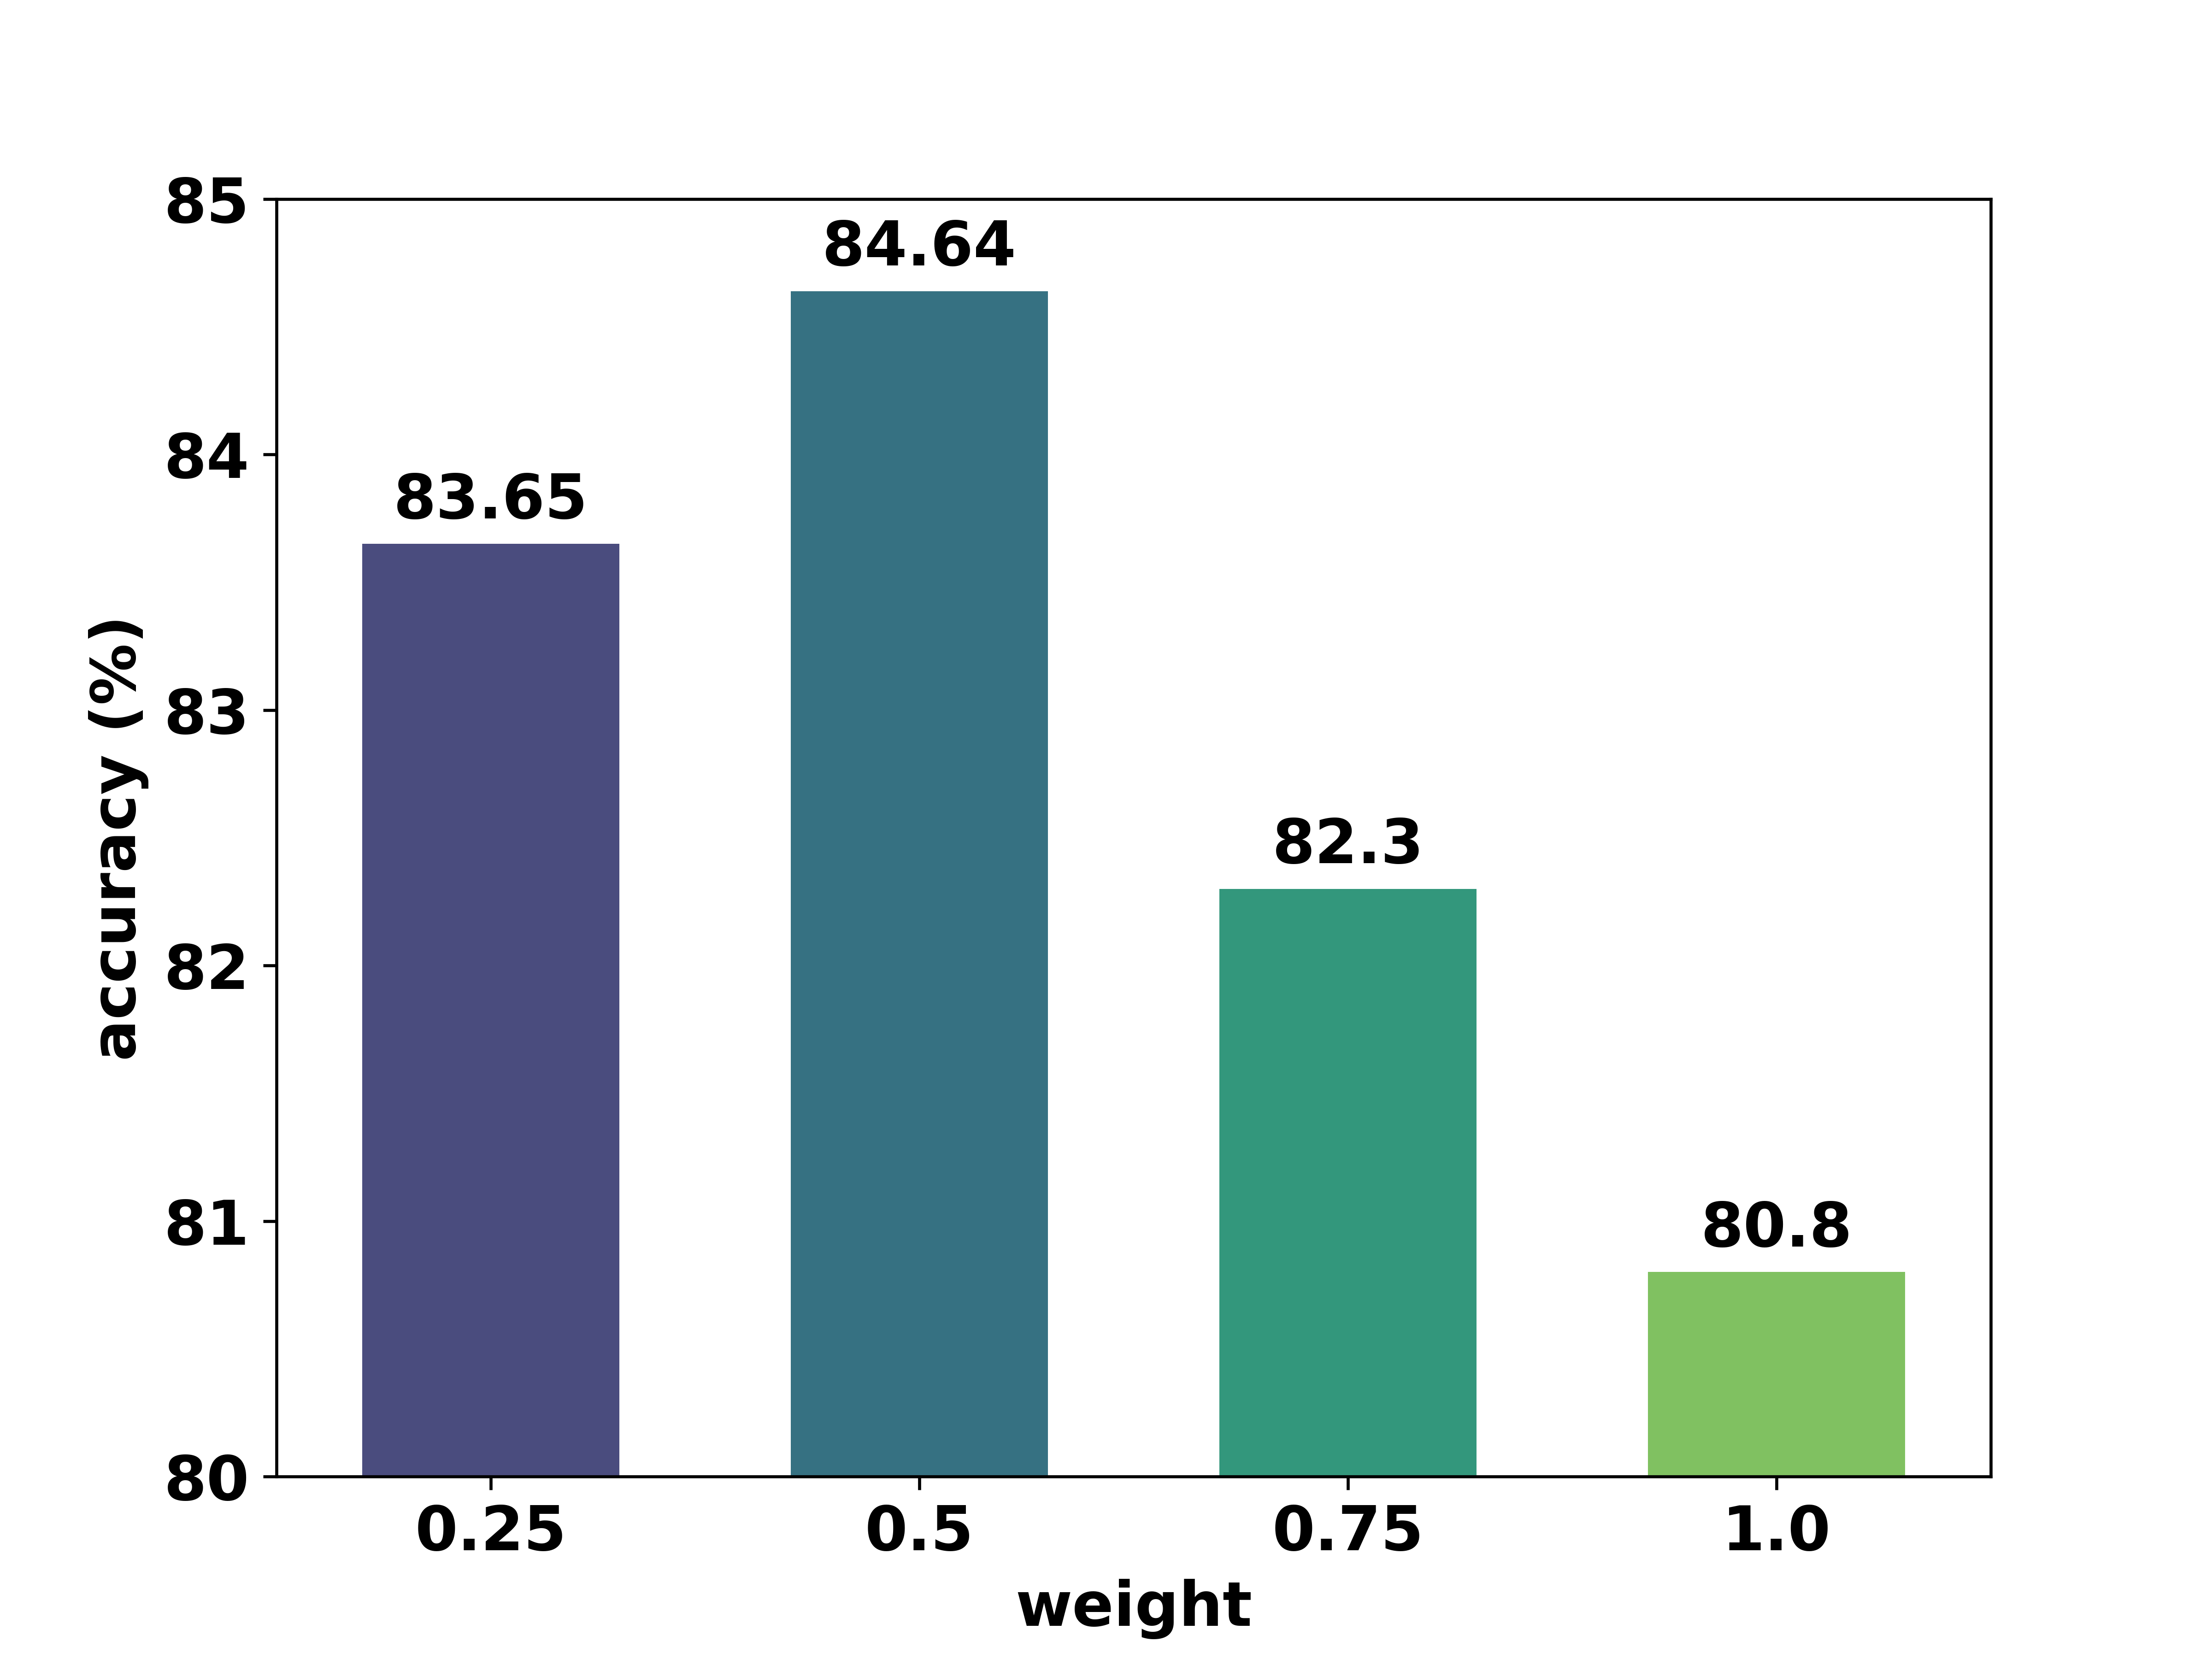
\includegraphics[width=\linewidth]{FIGURES/rlpl/accuracy_vs_weight.png}
    \caption{Effect of the auxiliary loss weight, $\lambda$.}
    \label{fig:weight}
\end{subfigure}%
\hspace{0.05\textwidth} % Adjust space here
\begin{subfigure}[t]{0.45\textwidth}
    \centering
    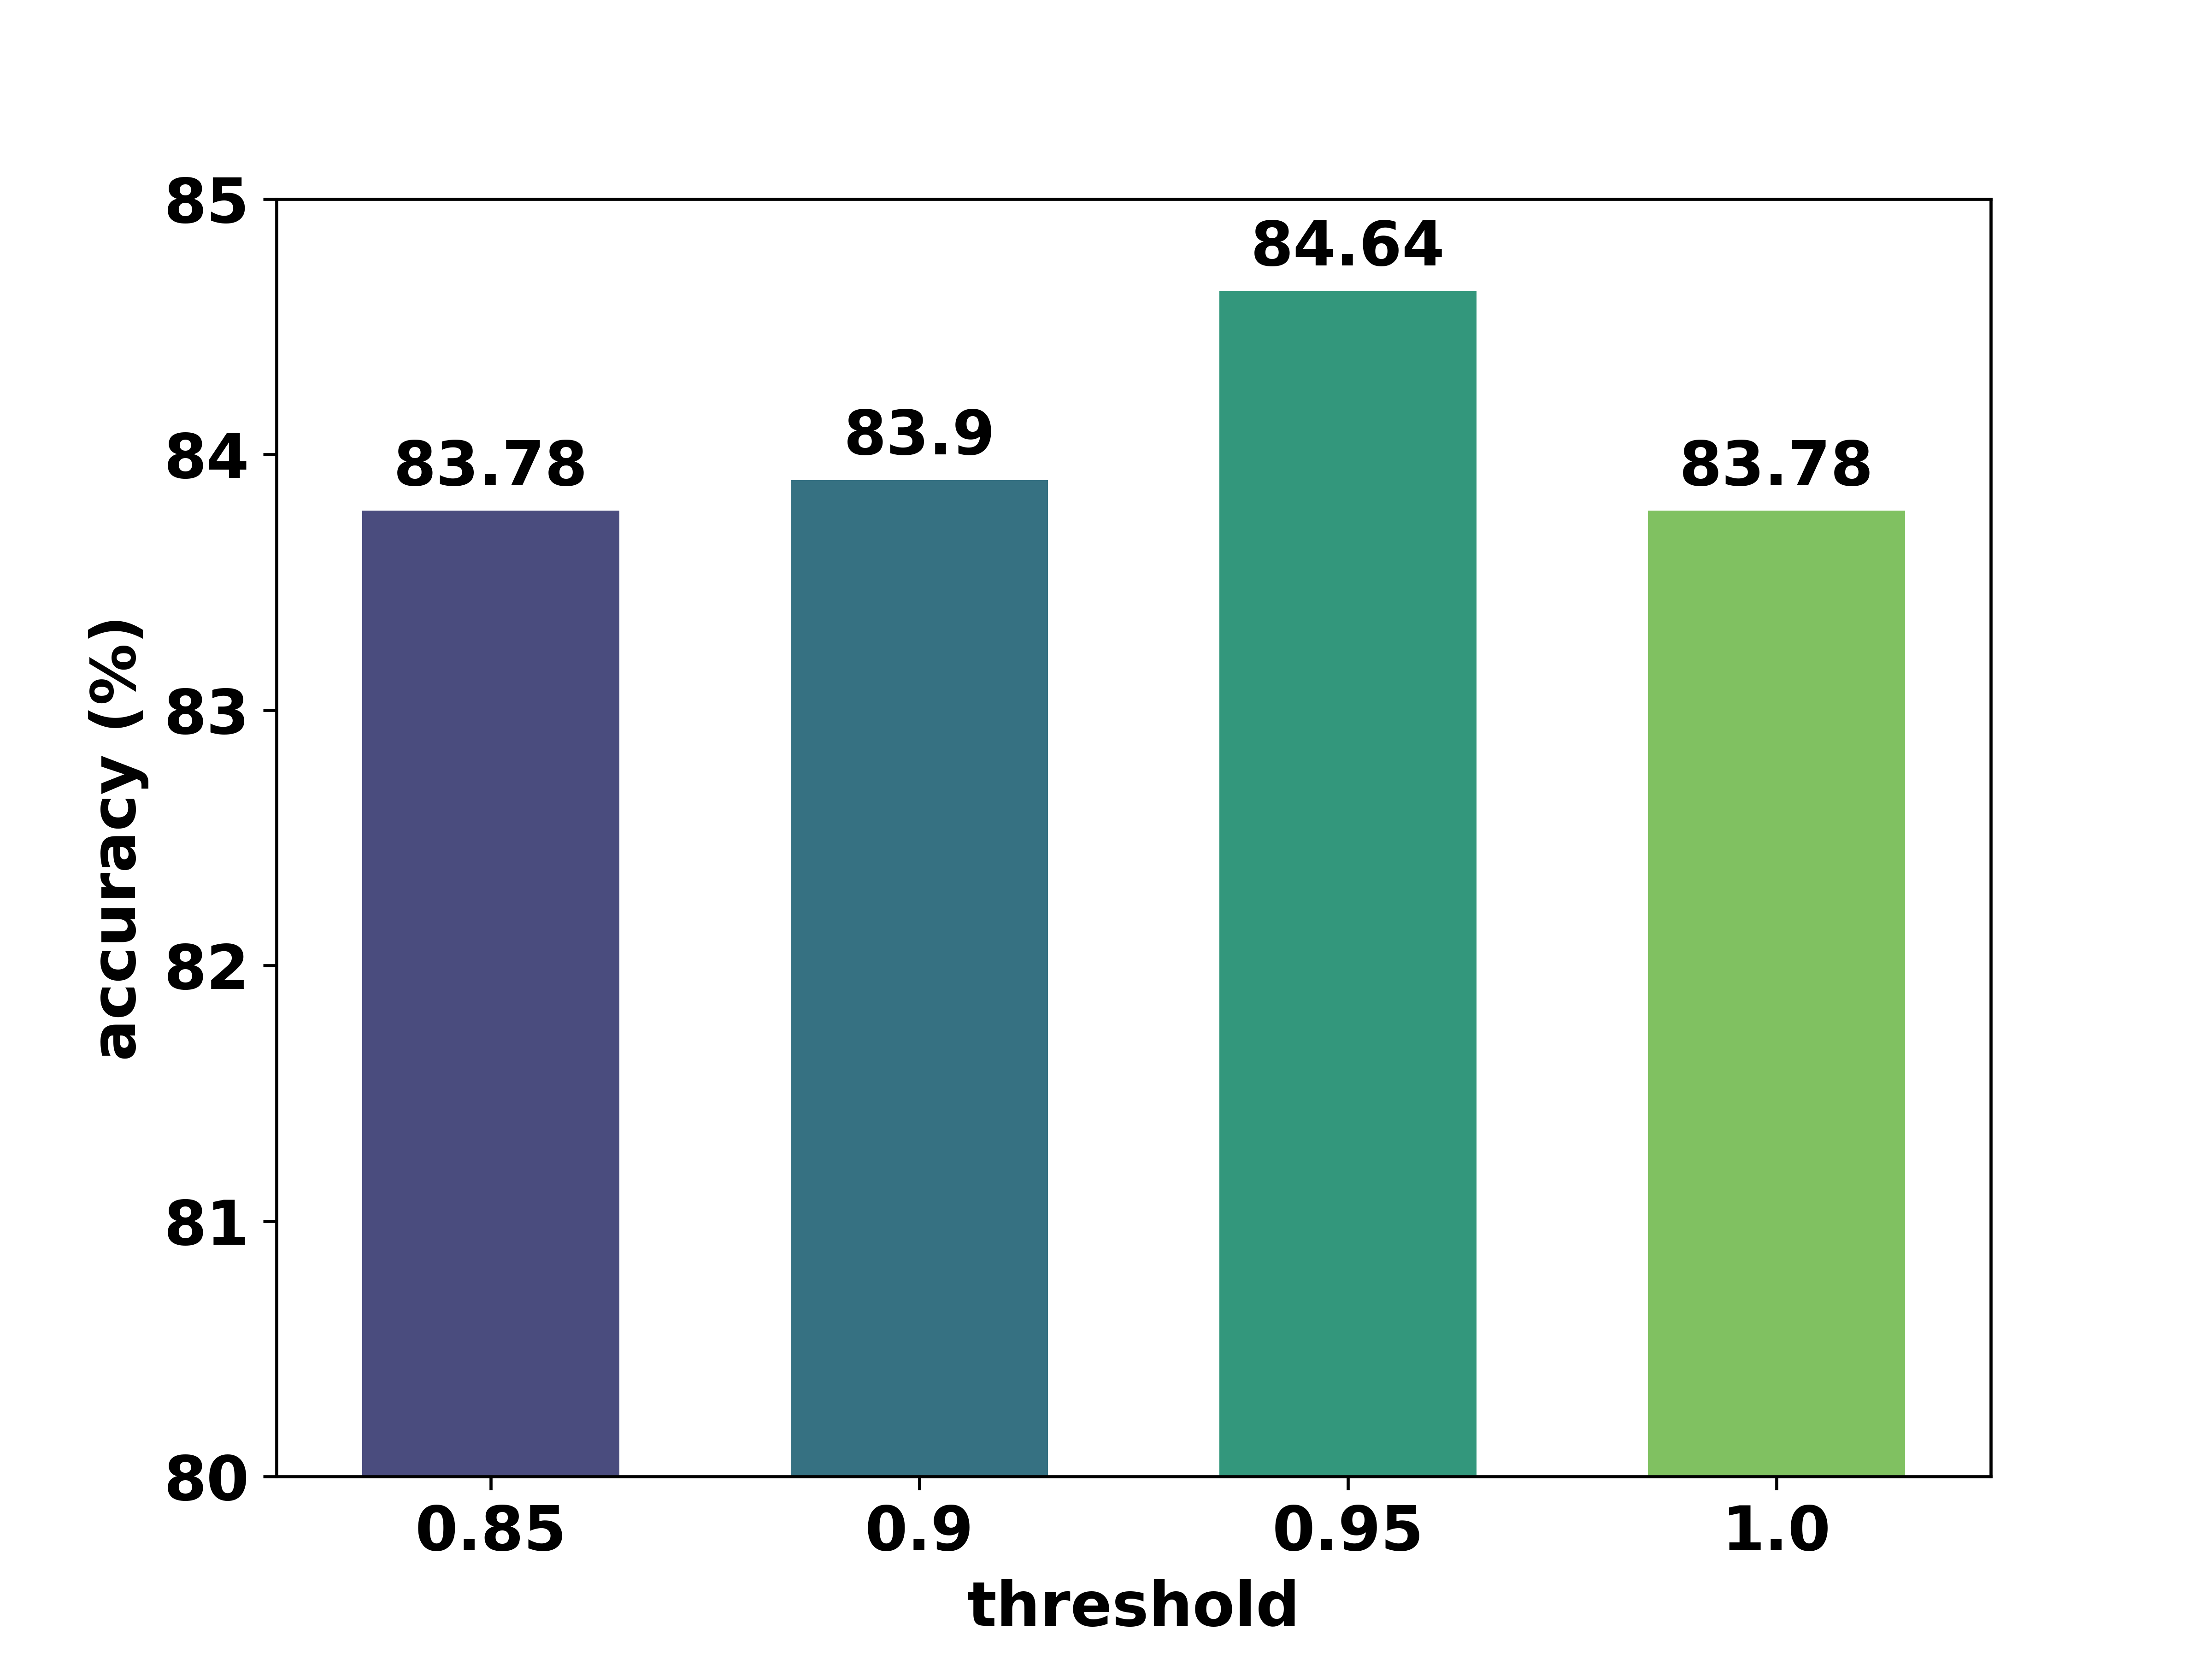
\includegraphics[width=\linewidth]{FIGURES/rlpl/accuracy_vs_threshold.png}
    \caption{Effect of the pseudo labels threshold, $\tau$.}
    \label{fig:threshold}
\end{subfigure}
\caption{Effects of different hyperparameters on model performance.}
\end{figure}

We conduct extensive ablation studies to evaluate the effectiveness of our method against the PL algorithm with random initialization and RLPL without PLs. Results in Table \ref{table:ablation} demonstrate the consistent superiority of RLPL across diverse datasets and label regimes. The PL with random initialization exhibits limited performance, particularly struggling with low-label scenarios (e.g., 30.49\% and 11.19\% accuracy with 250 labels), highlighting the importance of proper initialization for PL's reliability. 

RLPL without pseudo labeling shows substantial improvements over the baseline, achieving gains on STL-10 (83.20\% vs 53.34\%) and SVHN (71.25\% vs 11.19\%), validating the effectiveness of our representation learning strategy. The full RLPL framework, integrating both representation learning and pseudo labeling, consistently achieves the highest performance across all configurations, with particularly strong improvements in low-label settings (e.g., 48.93\% on CIFAR-10 with 250 labels, an 18.44\% improvement). This comprehensive performance advantage is reflected in the average accuracy across all settings, demonstrating RLPL's robust capability, especially in label-scarce scenarios where traditional approaches typically falter.

\subsection{Ablation on Noisy Teacher}

\begin{table}[!htbp]
\centering
\begin{tabular}{cc}
\hline
\textbf{Method} & \textbf{Accuracy (\%)} \\
\hline
Noisy Student    & 84.54 $\pm$ 0.05 \\
Noiseless Teacher & 84.59 $\pm$ 0.02 \\
Noisy Teacher     & 84.63 $\pm$ 0.02 \\
\hline
\end{tabular}
\caption{Input types ablation for pseudo labeling.}
\label{table:noise}
\end{table}
We investigate the impact of noisy samples (weakly augmented) in both teacher and student networks. Table~\ref{table:noise} shows the average performance of five different runs for three configurations: the noisy student, the noiseless teacher, and our proposed noisy teacher method. While the differences are subtle, they reveal interesting patterns in model behavior. The noisy student achieves 84.54\% accuracy with a standard deviation of 0.05, suggesting some variability in performance. When we remove noisy samples from the teacher network, we observe a marginal improvement to 84.59\% with reduced variance. Our proposed approach achieves the highest accuracy at 84.63\% with consistently low variance. These results suggest that weak augmentation in the teacher network inputs can provide additional regularization benefits.


% \subsection{Projector Dimensionality}
\subsection{Parameter Studies}

We conduct parameter sensitivity studies to examine the impact of key hyperparameters on RLPL's performance, focusing on the auxiliary loss weight and pseudo-label threshold. These studies help validate our design choices and provide insights for optimal configuration.

\subsubsection{Weight of the Auxiliary Loss}

We modify the weight of auxiliary loss, $\lambda$, from $0.25$ to $1.0$ with an increment of $0.25$. We observe that there is a strong effect of the weight on model performance. For weights other than $0.50$, the test accuracy declines as we move further from this value. The outputs are shown in Figure \ref{fig:weight}.

\subsubsection{Threshold for Pseudo Labels}

We vary the threshold, $\tau$, from $0.85$ to $1.0$ with an increment of $0.05$. We observe that the highest accuracy is obtained at $0.95$, and it keeps decreasing for a lower threshold value. Again, the accuracy decreases for a threshold value of $1.0$. For any threshold other than $0.95$, the accuracy drops below 84.0\%. The outputs are shown in Figure \ref{fig:threshold}.

\subsection{Conclusion}

We present RLPL, a novel semi-supervised learning framework that maximizes unlabeled data utility while addressing limitations in existing methods. RLPL achieves consistent improvements over SOTA methods with smaller batch sizes, enhancing efficiency in memory-constrained environments. Our experiments demonstrate substantial performance gains across multiple datasets, particularly with limited labeled data. RLPL also shows exceptional transferability across diverse downstream classification tasks without requiring pseudo labels for adaptation. These advantages in data efficiency, robustness, and generalization make RLPL particularly valuable for applications demanding memory efficiency and cross-task adaptability.

\section{Overall Findings}

In this chapter, we have explored maximizing unlabeled data utility in machine learning through advanced semi-supervised learning techniques, with particular focus on their role in enabling practical wireless foundation models. Our investigation has yielded several important findings that contribute to both theoretical understanding and practical application of SSL methods in the context of our three-stage foundation model framework.

\textbf{Fundamental limitations identified:} Existing representation learning approaches depend on large batch sizes and fail to effectively leverage unlabeled data during downstream tasks. These limitations create barriers to deployment in resource-constrained wireless environments and prevent full utilization of the abundant unlabeled signals available in spectrum monitoring scenarios. For wireless foundation models, these constraints are particularly critical since edge deployment often involves limited computational resources.

\textbf{RLPL framework contributions:} Our proposed RLPL (Representation Learning with Pseudo-Labeling) framework addresses these limitations through a two-phase approach combining improved representation learning with meta-pseudo-labeling. The key innovation in the representation learning phase is incorporating auxiliary loss functions that extract additional information from each training sample, enabling stable learning even with smaller batch sizes. This demonstrates that effective representation learning need not depend on massive computational resources—critical for wireless foundation model deployment on resource-constrained hardware.

The meta-pseudo-labeling component further enhances model performance by creating a feedback loop between teacher and student networks, significantly improving pseudo-label quality in low-supervision regimes where traditional pseudo-labeling methods struggle. For wireless signals, where obtaining expert annotations for every modulation scheme across all SNR conditions is prohibitively expensive, this capability to learn from high-quality pseudo-labels is essential. By combining strong initialization from representation learning with refined pseudo-label generation, RLPL creates a synergistic effect that maximizes information extraction from unlabeled data.

\textbf{Experimental validation:} Extensive evaluation confirms that RLPL consistently outperforms state-of-the-art methods across diverse datasets and supervision levels. Performance improvements are most pronounced in extremely label-scarce scenarios (e.g., CIFAR-10 with only 250 labels, achieving up to 15.74\% accuracy gains), directly relevant to wireless scenarios where collecting labeled modulation data at scale is impractical. Additionally, RLPL demonstrates excellent transferability across heterogeneous downstream tasks without requiring task-specific adaptations—aligning with the foundation model principle of learning general-purpose representations that transfer broadly.

\textbf{Robustness and ablation insights:} Parameter sensitivity studies reveal that RLPL's performance is robust across a range of hyperparameter values, with optimal configurations for the auxiliary loss weight ($\lambda=0.5$) and pseudo-label threshold ($\tau=0.95$) providing consistent improvements. Ablation studies confirm that both components contribute meaningfully to final performance, with their combination yielding the strongest results.

\textbf{Foundation model implications:} This chapter demonstrates how semi-supervised learning serves as a critical enabling methodology for wireless foundation models. RLPL allows Stage 1 (self-supervised pre-training, Chapter 2) to operate effectively with minimal labeled data by maximizing unlabeled signal utilization. It enhances Stage 2 (meta-learning adaptation, Chapter 3) by providing high-quality pseudo-labeled samples that augment few-shot learning episodes. Together, these capabilities address the fundamental data bottleneck in wireless AI: abundant unlabeled signals but scarce expert annotations.

The demonstrated performance gains suggest that SSL approaches like RLPL can significantly reduce annotation requirements while maintaining high model accuracy, addressing a critical bottleneck in deploying wireless foundation models at scale. By enabling effective learning from limited labels and abundant unlabeled data, RLPL makes the three-stage foundation model framework practical for real-world wireless applications.

\textbf{Pathway forward:} The principles and techniques presented in this chapter provide a foundation for developing more data-efficient, accessible wireless foundation models capable of operating effectively with varying levels of supervision. With Stages 1-2 (pre-training + adaptation) now established through Chapters 2-4, the next chapter (Chapter 5) completes our vision by integrating these learned representations with large language models to enable true open-set recognition—moving beyond closed-set classification to general-purpose wireless intelligence.


%%%%%%%%%%%%%%%%%%%%%%%%%%%%%%%%%%%%%%%%%%%%%%%%%%%%%%%%%%%%%%%%%%%%%%%%%
%
%	LaTeX File for Stanford University PhD Thesis
%
%%%%%%%%%%%%%%%%%%%%%%%%%%%%%%%%%%%%%%%%%%%%%%%%%%%%%%%%%%%%%%%%%%%%%%%%%
%	Copyright 2001  by  Jung-Suk Goo    (goojs@gloworm.stanford.edu)
%%%%%%%%%%%%%%%%%%%%%%%%%%%%%%%%%%%%%%%%%%%%%%%%%%%%%%%%%%%%%%%%%%%%%%%%%

\chapter{Conclusions and Future Work}
\label{chap:concl}

\section{Conclusions}

This dissertation has explored the development of wireless physical foundation models that integrate self-supervised representation learning, meta-learning for rapid adaptation, and large language model reasoning for open-set recognition. The primary goal has been to address critical challenges in building general-purpose AI systems for wireless signals: learning from unlabeled data, adapting quickly with minimal supervision, and generalizing to unseen modulation schemes beyond the training distribution. Our research has produced a three-stage framework demonstrating that wireless signals can exhibit the same foundation model capabilities—pre-training on broad data, rapid task adaptation, and open-ended reasoning—that have transformed natural language processing and computer vision.

\textbf{Stage 1: Self-Supervised Pre-Training for Wireless Signals (Chapter 2)}

Our first major contribution addresses automatic modulation classification (AMC) through self-supervised representation learning, establishing the foundation for wireless foundation models. \textbf{NMformer} demonstrated that Vision Transformers can effectively process constellation diagrams, achieving high accuracy across diverse noise conditions without explicit denoising. The pre-train-then-fine-tune paradigm showed that models trained on broad datasets rapidly adapt to specific SNR regimes with limited data—exhibiting the generalization and sample efficiency characteristic of foundation models.

\textbf{DenoMAE}, our primary Stage 1 contribution, introduced a multimodal masked autoencoder framework that treats noise as an explicit modality, pre-training on unlabeled signals across time-domain and constellation representations. This self-supervised approach achieved remarkable data efficiency: requiring 10× less unlabeled pre-training data and 3× less labeled fine-tuning data compared to supervised methods. DenoMAE's learned encodings serve as semantic features for LLM-based open-set recognition (Chapter 5), bridging self-supervised signal representation learning with natural language reasoning. This positions DenoMAE as the core pre-training stage in our wireless foundation model pipeline.

These methodologies collectively demonstrate that transformer architectures and masked autoencoders—the building blocks of foundation models in NLP and vision—can be successfully adapted to wireless physical signals, achieving robustness, data efficiency, and transferability across SNR regimes.

\textbf{Stage 2: Meta-Learning for Rapid Task Adaptation (Chapter 3)}

In the realm of few-shot and meta-learning, we introduced \textbf{BEpiC}, \textbf{MetaRep}, and \textbf{Meta-Task} to enable rapid adaptation with minimal labeled data—the hallmark of foundation models. BEpiC improved cross-domain generalization through binary episode construction, encouraging learning of domain-invariant representations that transfer robustly across different task distributions. For wireless signals, this translates to better generalization across SNR regimes and channel conditions.

MetaRep advanced meta-learning by learning episodic representations through task-conditioned feature modulation, enabling effective few-shot classification by dynamically adapting features based on the support set. This aligns with the foundation model principle of learning general-purpose representations that can be rapidly specialized for specific tasks. Meta-Task introduced method-agnostic learnable regularization, showing that adaptive regularization improves few-shot generalization across diverse meta-learning algorithms—critical for foundation models that must be robust to various deployment scenarios.

Collectively, these contributions demonstrate that meta-learning serves as the critical adaptation layer (Stage 2) in our wireless foundation model framework. Given pre-trained representations from DenoMAE (Stage 1), these techniques enable rapid specialization to new modulation schemes, SNR regimes, or signal environments with minimal labeled data—the sample efficiency required for practical deployment.

\textbf{Practical Training Methodology: Semi-Supervised Learning (Chapter 4)}

We explored maximizing unlabeled data utility via semi-supervised learning through \textbf{RLPL} (Representation Learning with Pseudo-Labeling), our novel framework combining improved representation learning with meta-pseudo-labeling. RLPL demonstrated exceptional performance in extremely label-scarce scenarios (up to 15.74\% accuracy gains with only 250 labels on CIFAR-10), directly addressing the data bottleneck in wireless AI: abundant unlabeled spectrum monitoring signals but scarce expert annotations.

RLPL serves as the practical training methodology enabling Stages 1-2 to operate effectively with minimal labeled data. It allows DenoMAE pre-training to maximize unlabeled signal utilization and enhances meta-learning adaptation by providing high-quality pseudo-labeled samples that augment few-shot episodes. This capability makes the three-stage foundation model framework viable for real-world wireless applications where collecting labeled data at scale is prohibitively expensive.

\textbf{Stage 3: LLM Integration for Open-Set Recognition (Chapter 5)}

\textit{[Note: Chapter 5 represents the culminating contribution of this thesis—integrating DenoMAE-learned encodings with large language models to enable open-set modulation recognition. While the implementation details appear in Chapter 5, the conceptual foundation was established through Stages 1-2: DenoMAE provides semantic wireless signal representations; meta-learning demonstrates rapid adaptation; and LLMs provide the reasoning capability to recognize modulations never seen during training by grounding signal features in natural language descriptions of modulation properties.]}

This novel integration bridges the gap between wireless physical signals and language-based reasoning, enabling zero-shot and few-shot recognition of unseen modulation schemes—moving beyond closed-set classification to truly general-purpose wireless intelligence. By treating DenoMAE encodings as "language" that LLMs can reason about, we demonstrate that foundation model capabilities extend to wireless signals, achieving the open-ended generalization that defines foundation models in other domains.

\textbf{Key Insights and Unified Vision}

Throughout this research, several key insights have emerged that collectively establish wireless foundation models as viable:

\begin{itemize}
\item \textbf{Transformer architectures} (Vision Transformers) excel at capturing global patterns in wireless signals, particularly when pre-trained on broad data distributions and fine-tuned for specific tasks—directly mirroring the foundation model paradigm in vision.

\item \textbf{Self-supervised masked autoencoding} on multimodal wireless signals (treating noise as a modality) learns transferable representations with minimal labeled data, achieving the sample efficiency required for foundation model pre-training.

\item \textbf{Meta-learning} enables rapid adaptation to new tasks with few examples, demonstrating that pre-trained wireless representations can be quickly specialized—the adaptability characteristic of foundation models.

\item \textbf{Semi-supervised learning} provides the practical training methodology for maximizing unlabeled data utilization, addressing the data scarcity bottleneck in wireless AI and making foundation model development economically viable.

\item \textbf{LLM integration} (Chapter 5) demonstrates that learned wireless signal representations can serve as semantic features for language-based reasoning, enabling open-set recognition and moving beyond fixed classification taxonomies toward general-purpose wireless intelligence.
\end{itemize}

The central contribution of this dissertation is demonstrating that wireless physical signals can be treated analogously to language or vision in foundation models: pre-train on unlabeled signals via masked autoencoders (Stage 1), rapidly adapt to new tasks via meta-learning (Stage 2), and enable open-ended reasoning through LLM integration (Stage 3). This three-stage framework establishes a pathway from traditional supervised AMC toward truly general-purpose wireless foundation models capable of recognizing, reasoning about, and adapting to novel signal environments.

\section{Future Work}

Building upon the contributions of this thesis, several promising research directions could further advance wireless foundation models toward truly general-purpose wireless intelligence. The following avenues represent significant opportunities for extending our three-stage framework:

\noindent \textbf{Advancing Stage 1: Pre-Training at Scale}

\begin{itemize}
    \item \textbf{Large-Scale Pre-Training Datasets:} Develop comprehensive wireless signal datasets spanning diverse modulation families, protocol standards (LTE, 5G, WiFi, satellite), and environmental conditions. Foundation models in NLP and vision benefited from web-scale pre-training (GPT-3: 300B tokens, CLIP: 400M image-text pairs); wireless foundation models similarly require orders-of-magnitude larger and more diverse pre-training corpora to achieve comparable generalization.
    
    \item \textbf{Advanced Signal Representations:} Extend DenoMAE to incorporate time-frequency representations beyond constellation diagrams—wavelet scalograms, cyclostationary feature maps, spectrograms—enabling multimodal pre-training across complementary signal views analogous to CLIP's vision-language training.
    
    \item \textbf{Real-World Validation:} Transition from synthetic datasets to real-world signals acquired from operational networks, software-defined radios, and multi-antenna systems. This addresses practical challenges including hardware impairments, non-Gaussian noise distributions, realistic interference patterns, and dynamic propagation environments—critical for operational deployment of wireless foundation models.
    
    \item \textbf{Scaling Laws for Wireless Signals:} Empirically characterize scaling laws relating model size, dataset size, and compute to performance on wireless tasks, analogous to Kaplan et al.'s analysis for language models. Understanding these relationships would guide efficient allocation of resources in developing larger wireless foundation models.
\end{itemize}

\noindent \textbf{Enhancing Stage 2: Meta-Learning and Adaptation}

\begin{itemize}
    
    \item \textbf{Transformer-Based Meta-Learning:} Integrate Meta-Task framework with Vision Transformers using specialized masked pre-training objectives tailored for signal processing. This hybrid approach could leverage global context capabilities while maintaining adaptation benefits, potentially enabling in-context learning where models adapt to new modulation schemes within the forward pass (analogous to GPT-3 few-shot prompting).
    
    \item \textbf{Continual Learning for Dynamic Spectrums:} Develop continual meta-learning approaches that enable wireless foundation models to incrementally learn new modulation schemes without catastrophic forgetting, addressing the dynamic nature of wireless protocols where new standards emerge continuously.
    
    \item \textbf{Few-Shot Model Compression:} Explore techniques to distill knowledge from complex meta-learned representations into compact models suitable for edge deployment, maintaining rapid adaptation capabilities while reducing computational requirements for resource-constrained IoT devices.
\end{itemize}

\noindent \textbf{Extending Stage 3: LLM Integration and Open-Set Recognition}

\begin{itemize}

    \item \textbf{Multimodal Language Grounding:} Develop richer language descriptions of wireless signal properties—symbol geometry, spectral characteristics, temporal patterns—enabling more nuanced LLM reasoning. This could involve automatically generating textual explanations of modulation features from DenoMAE encodings, creating a bidirectional bridge between signals and language.
    
    \item \textbf{Zero-Shot Protocol Understanding:} Extend LLM integration beyond modulation classification to protocol decoding, spectrum policy reasoning, and interference diagnosis. By grounding wireless domain knowledge in language models, foundation models could reason about entirely new communication protocols from textual specifications alone—true zero-shot generalization.
    
    \item \textbf{Interactive Spectrum Intelligence:} Build conversational AI systems where users can query wireless foundation models in natural language ("Identify unusual signals in the 2.4 GHz band," "Explain why this link fails at low SNR"), enabling intuitive human-AI collaboration for spectrum monitoring and network troubleshooting.
\end{itemize}

\noindent \textbf{Cross-Cutting Directions: Toward General Wireless Intelligence}

\begin{itemize}
    \item \textbf{Unified Wireless-Vision-Language Models:} Develop joint foundation models that simultaneously process wireless signals, visual data (e.g., environment sensing), and natural language, enabling multimodal reasoning for applications like autonomous vehicles (fusing radar, camera, communication signals) or smart cities (integrated sensing-communication systems).
    
    \item \textbf{Foundation Models for Physical Layer Security:} Apply the three-stage framework to adversarial signal environments—pre-train on benign/adversarial signal distributions, rapidly adapt to detect novel spoofing or jamming attacks via meta-learning, use LLM reasoning to explain attack signatures and recommend countermeasures.
    
    \item \textbf{Federated Learning for Wireless Foundation Models:} Develop privacy-preserving distributed training methods enabling collaborative pre-training across organizations (telecom operators, defense agencies, research institutions) without sharing raw signal data, accelerating development of large-scale wireless foundation models while respecting data sovereignty.
    
    \item \textbf{Benchmarking Open-Set Wireless Intelligence:} Establish standardized evaluation protocols for wireless foundation models analogous to GLUE/SuperGLUE (NLP) or ImageNet (vision), including tasks spanning modulation recognition, protocol decoding, interference classification, spectrum forecasting, and cross-domain transfer—enabling rigorous comparison of foundation model capabilities.
\end{itemize}

\textbf{Broader Impact and Vision}

The research directions outlined above collectively point toward a future where wireless foundation models achieve the same transformative impact in spectrum management and wireless communication that language models (GPT, BERT) and vision models (CLIP, SAM) have achieved in their respective domains. Such models would:

\begin{itemize}
\item \textbf{Democratize wireless AI} by reducing the expertise and labeled data required to develop signal processing systems, enabling smaller organizations and researchers to build state-of-the-art wireless applications.

\item \textbf{Enable cognitive radios and dynamic spectrum access} that reason about novel signals and protocols on-the-fly, adapting to congested or adversarial spectrum environments without pre-programmed rules.

\item \textbf{Accelerate 6G research} by providing foundation models that quickly adapt to experimental waveforms, beamforming strategies, and modulation schemes, reducing the time from concept to deployment.

\item \textbf{Support spectrum policy and regulation} through AI systems that understand wireless signals in human terms, facilitating dialogue between engineers, policymakers, and the public about spectrum allocation and interference management.
\end{itemize}

This dissertation has laid the groundwork for this vision by demonstrating that wireless physical signals can be treated as a modality amenable to foundation model development. The three-stage framework—self-supervised pre-training, meta-learning adaptation, and LLM-based reasoning—provides a principled pathway from traditional signal processing toward general-purpose wireless intelligence. Future work must scale this approach to match the ambition that has driven foundation model development in language and vision, ultimately realizing truly universal models capable of understanding and reasoning about any wireless signal in any environment.



%--- Appendix -----------------------
\appendix
%%%%%%%%%%%%%%%%%%%%%%%%%%%%%%%%%%%%%%%%%%%%%%%%%%%%%%%%%%%%%%%%%%%%%%%%%
%
%	LaTeX File for Stanford University PhD Thesis
%
%%%%%%%%%%%%%%%%%%%%%%%%%%%%%%%%%%%%%%%%%%%%%%%%%%%%%%%%%%%%%%%%%%%%%%%%%
%	Copyright 2001  by  Jung-Suk Goo    (goojs@gloworm.stanford.edu)
%%%%%%%%%%%%%%%%%%%%%%%%%%%%%%%%%%%%%%%%%%%%%%%%%%%%%%%%%%%%%%%%%%%%%%%%%

\chapter{Chapter Title}
\label{chap:append1}



%--- Bibliography -------------------
\addcontentsline{toc}{chapter}{\bibname}
\bibliographystyle{SETUP/thesis_bib}
\bibliography{REFERENCE/reference}


%=== End Thesis ========================================
\end{thesis}
\end{document}
